\documentclass[12pt,draft]{article}
\usepackage{
  amsmath,
  amsthm,
  booktabs,
  flexisym,
  microtype,
  multicol,
  pgfplots,
  subfig,
  tabularx,
  tikz,
  url
}

\frenchspacing
\usepackage[round]{natbib}
\usepackage[margin=1.25in]{geometry}
\usepackage[charter]{mathdesign}
\usepackage[osf]{sourcecodepro}
\usepackage[multiple]{footmisc}
\DisableLigatures{family = tt*}
\urlstyle{same}
\newcolumntype{C}{>{\centering\arraybackslash}X}

\usetikzlibrary{calc}
\usetikzlibrary{fit}
\usepgfplotslibrary{external}
\tikzexternalize

\newtheorem{thm}{Theorem}
\newtheorem{lem}{Lemma}
\newtheorem{claim}{Claim}
\newtheorem{cor}{Corollary}
\newtheorem{asmp}{Assumption}
\newtheorem{example}{Example}
\newtheorem{defn}{Definition}
\newtheorem{innercustomasmp}{Assumption}
\newenvironment{customasmp}[1]
  {\renewcommand\theinnercustomasmp{#1}\innercustomasmp}
  {\endinnercustomasmp}

\newcommand{\citepos}[1]{\citeauthor{#1}'s \citeyearpar{#1}}
\newcommand{\Citepos}[1]{\Citeauthor{#1}'s \citeyearpar{#1}}
\newcommand{\clws}{\citeauthor{ClW:06}'s \citeyearpar{ClW:06,ClW:07}}

\DeclareMathOperator{\1}{1}
\DeclareMathOperator*{\argmin}{arg\,min}
\DeclareMathOperator{\atan}{atan*}
\DeclareMathOperator{\cov}{cov}
\DeclareMathOperator{\E}{E}
\DeclareMathOperator{\eigen}{\lambda}
\DeclareMathOperator*{\plim}{plim}
\DeclareMathOperator*{\rank}{rank}
\DeclareMathOperator{\tr}{tr}
\DeclareMathOperator{\var}{var}

\newcommand{\e}{\varepsilon}
\newcommand{\eb}{\mathbf{\e}}
\newcommand{\mbig}{\,\big|\,}
\newcommand{\mBig}{\,\Big|\,}

\newcommand{\tryinput}[2][{}]{\IfFileExists{#2}{\input{#2}}{#1}}

\newcommand{\sh}{\hat{\sigma}}
\newcommand{\oosA}{\bar{D}_{R}}
\newcommand{\oosB}{\bar{D}_{T}}

\newcommand{\oost}{\ensuremath{\operatorname{OOS-\mathit{t}}}}
\newcommand{\oosSum}[2]{\ensuremath{\sum_{#1=R+#2}^{T-\h}}}

\newcommand{\h}{h}
\newcommand{\InnerBlockL}[1]{\ensuremath{R+(#1-1)b_T + 1}}
\newcommand{\InnerBlockU}[1]{\ensuremath{R+#1 b_T}}
\newcommand{\OuterBlockU}{\lfloor P/b_T \rfloor}
\newcommand{\SumOuterBlock}[1]{\ensuremath{\sum_{#1=1}^{\OuterBlockU}}}
\newcommand{\SumInnerBlock}[2]{\ensuremath{\sum_{#1=\InnerBlockL{#2}}^{\InnerBlockU{#2}}}}

\newcommand{\CEOuterBlock}[2]{\ensuremath{\E_{\InnerBlockU{(#2-1)}} #1}}

\newcommand{\ZSummand}{D_s - \E_R D_s}
\newcommand{\ZDef}{P^{-1/2} \SumInnerBlock{s}{i} [\ZSummand]}
\newcommand{\ZSqCE}{\ensuremath{\CEOuterBlock{Z_i^2}{i}}}
\newcommand{\ZTrunc}{\ensuremath{C\sqrt{b_{T}/P}}}
\newcommand{\PScaleTerm}{\ensuremath{\frac{C \sqrt{b_T}}{P}}}

\newcommand{\vWeight}{W((t-s)/\gamma)}
\newcommand{\vSummand}{\ensuremath{(D_t - \E_R D_t)(D_s - \E_R D_s) \vWeight}}
\newcommand{\kernelBDefn}[1]{\ensuremath{\delta^{-1}(2\pi)^{-1/2}}e^{-#1^2/2\delta^2}}
\newcommand{\kernelB}[1]{\ensuremath{\eta_{\delta}(#1)}}

\newcommand{\vtSum}{\ensuremath{\sum_{t=-P+R+1}^{2P+R}}}
\newcommand{\vtSumr}{\ensuremath{\sum_{i=1}^r}}
\newcommand{\vtSuma}{\ensuremath{\sum_{t=(2i-2)b_T-P+R+1}^{(2i-1)b_T-P+R}}}
\newcommand{\vtSumb}{\ensuremath{\sum_{t=(2i-1)b_T-P+R+1}^{2ib_T-P+R}}}
\newcommand{\vttLower}{\ensuremath{\max(R+1-t,-b_T)}}
\newcommand{\vttUpper}{\ensuremath{\min(R+P-t,b_T)}}

\newcommand{\varianceTermIDefn}{\ensuremath{P^{-1}\oosSum{s,t}{1}
    \vSummand}}
\newcommand{\varianceTermI}{\ensuremath{\sigma_{0,\delta}^2}}
\newcommand{\varianceTermII}{\ensuremath{\sigma_{1,\delta}^2}}
\newcommand{\varianceTermIIa}{\ensuremath{(P\gamma)^{-1/2}
    \sum_{l=\max(1-t,-P)}^{\min(P-t,P)} (D_{t+l+R} - \E_R D_{t+l+R})
    W(l/\gamma)}}
\newcommand{\varianceTermIIb}{\ensuremath{(P\gamma)^{-1/2}
    \sum_{j=1-t}^{P-t} (D_{t+j+R} - \E_R D_{t+j+R})
    \kernelB{j/\gamma}}}
\newcommand{\varianceTermIII}{\ensuremath{\sigma_{2,\delta}^{2}}}
\newcommand{\varianceTermIIIa}{\ensuremath{(P\gamma)^{-1/2}
    \sum_{l=\vttLower}^{\vttUpper} (D_{t+l} - \E_R D_{t+l}) W(l/\gamma)}}
\newcommand{\varianceTermIV}{\ensuremath{\sigma_{3,\delta}^{2}}}
\newcommand{\varianceTermIVb}{\ensuremath{(P\gamma)^{-1/2}
    \sum_{j=\vttLower}^{\vttUpper} (D_{t+j} - \E_R D_{t+j})
    \kernelB{j/\gamma}}}
\newcommand{\vtIIIsummand}{\ensuremath{(Z_{1t}Z_{2t} - \E_RZ_{1t}Z_{2t})}}

\newcommand{\varianceDiffA}{\ensuremath{P^{-1} \oosSum{s,t}{1}
    \lvert (D_s - \E_R D_s)(\E_R D_t - \oosA) \rvert
    \vWeight}}
\newcommand{\varianceDiffAi}{\ensuremath{P^{-1} \oosSum{s}{1}(\E_R
    D_s - \oosA )^2}}
\newcommand{\varianceDiffAii}{\ensuremath{P^{-1} \oosSum{s}{1}
    (D_s - \E_R D_s)^2}}

\newcommand{\rhoExp}{\ensuremath{(\rho-2)/2\rho}}
\newcommand{\absReg}{\ensuremath{\rho/(\rho-2)}}

\newcommand{\couplingConstant}{\ensuremath{2^{(1+\rho)/\rho} B_L}}
\newcommand{\couplingBeta}[1]{\ensuremath{\beta^{(\rho-2)/2\rho}_{#1}}}
\newcommand{\couplingBetaSq}[1]{\ensuremath{\beta^{(\rho-2)/\rho}_{#1}}}
\newcommand{\couplingBound}[1]{\couplingConstant \, \couplingBeta{#1}}

\newcommand{\OCoef}{\ensuremath{O_p(\frac{\sqrt{P}}{T})}}

\newcommand{\bh}[1]{\ensuremath{\hat\theta_{#1}}}
\newcommand{\ep}[1]{\ensuremath{\boldsymbol{\varepsilon}_{#1}}}

\newcommand{\olsMatrix}[2]{\ensuremath{(#1'#1)^{-1}#1'#2}}

\newcommand{\sfield}{$\sigma$-field}
\newcommand{\sfields}{\sfield s}
\renewcommand{\Re}{\ensuremath{\mathbb{R}}}
\newcommand{\Gs}{\mathcal{G}}
\newcommand{\Fs}{\mathcal{F}}

%%% Local Variables: 
%%% mode: latex
%%% TeX-master: paper.tex
%%% End: 


\title{Out-of-Sample Comparisons of Overfit Models}
\author{Gray Calhoun\thanks{email: gcalhoun@iastate.edu. I
    would like to thank Julian Betts, Helle Bunzel,
    St\'ephane Bonhomme, Marjorie Flavin,
    Nir Jaimovich, Lutz Kilian, Ivana Komunjer, Michael McCracken,
    Seth Pruitt, Ross Starr, Jim Stock, Yixiao Sun, Allan Timmermann,
    Hal White, several anonymous referees, participants at the 2010
    Midwest Economics Association Annual Meetings, the 2010
    International Symposium on Forecasting, the 2010 Joint Statistical
    Meetings, the 2011 NBER-NSF Time-Series
    Conference, and in many seminars at UCSD, and especially
    Graham Elliott for their valuable suggestions, feedback and advice
    in writing this paper.  I would also like to thank Amit Goyal for
    providing computer code and data for his 2008 RFS paper
    with Ivo Welch \citep{GoW:08}.} \\ Iowa State University}

\date{\VERSION}

\begin{document}
\maketitle

\begin{abstract}\noindent
  This paper uses dimension asymptotics to study the behavior of
  out-of-sample (OOS) test statistics when they are used to compare
  ``overfit'' linear regression models. Under these asymptotics, the
  number of predictors used by the larger model increases with the
  number of observations so that their ratio remains uniformly
  positive. This analysis gives a theoretical motivation for using
  out-of-sample (OOS) comparisons: the Diebold-Mariano-West OOS $t$-test
  (Diebold and Mariano, 1995, \textit{JBES}, and West, 1996,
  \textit{Econometrica}) allows a forecaster to conduct inference
  about the models' generalization error, an important measure of
  forecast accuracy that conditions on the models' parameter estimates.
  We show analytically and through Monte Carlo that standard full-sample
  test statistics can not test hypotheses about this measure of performance.
  Our paper also suggests that comparisons of overfit models require small
  OOS test samples. If $P$ denotes the number of observations used for the
  OOS comparison and $T$ the total number of observations, $P^2/T$ must
  converge to zero for the OOS $t$-test to be centered on the model's
  generalization error.

\noindent JEL Classification: C12, C22, C52, C53

\noindent Keywords: Generalization Error, Forecasting, Model
Selection, $t$-test, Dimension Asymptotics
\end{abstract}
\newpage

\section{Introduction}
\label{sec:introduction}

Consider two sequences of length $P$ of prediction errors, the result
of forecasting the same variable with two different estimated models.
Both models are estimated with $R$ observations, collectively called
the {\em estimation window}, and are used to forecast an additional
$P$ observations, called the {\em test sample}.  There are $T$
observations in all, and $R+P=T$.  This paper introduces a new limit
theory for statistics constructed from these prediction errors
designed to approximate the behavior of the statistics when one of the
models is overfit.  In doing so, we provide a theoretical
justification for forecasters to use out-of-sample (OOS) instead of in-sample
comparisons: the DMW OOS test\footnote{%
  In this paper, we will refer to the basic OOS $t$-test studied by
  \citet{DiM:95} and \citet{Wes:96} as the DMW test.} %
allows a forecaster to conduct
inference about the expected future accuracy of his or her models when
one or both is overfit.  We show analytically and through Monte Carlo simulations
that standard full-sample test statistics can not test hypotheses
about this performance.

Our paper also shows that popular test and training sample sizes may
give misleading results if researchers are concerned about overfit.
We show that $P^2/T$ must converge to zero for the DMW test to give
valid inference about the expected forecast accuracy, otherwise the
test measures the accuracy of the estimates constructed using only the
training sample.  In empirical research, $P$ is typically much larger
than this.  Our simulations indicate that using large values of $P$
with the DMW test gives undersized tests with low power, so this
practice may favor simple benchmark models too much.  Existing
corrections, proposed by \citet{ClM:01,ClM:05}, \citet{Mcc:07} and
\citet{ClW:06,ClW:07}, seem to overcorrect for this problem, though, and reject
too often when the benchmark model is more accurate.

Although OOS comparisons have been popular in Macroeconomics and
Finance since \citepos{MeR:83} seminal study of exchange rate models,
it has been unclear from a theoretical perspective whether or not the
statistics are useful.  Empirical researchers often cite ``overfit''
or ``instability'' as reasons for using OOS comparisons, as in
\citet{StW:03}, but neither term is precisely defined or formalized.
Compounding this problem, the asymptotic distributions of these
statistics are derived under conditions that rule out either
instability or overfit and allow a researcher to use a conventional
in-sample comparison---a variation of the $F$-test, for example.  As
\citet{InK:04} argue, the statistics themselves are designed to test
hypotheses that can be tested by these in-sample statistics.  For
example, \citet{DiM:95} and \citet{Wes:96} derive the limiting
distributions of many popular OOS test statistics under conditions
that would justify these full-sample tests.  Much
of the subsequent research by \citet{Mcc:00, Mcc:07}, \citet{CCS:01},
\citet{ClM:01,ClM:05}, \citet{CoS:02,CoS:04}, \citet{ClW:06,ClW:07},
\citet{Ana:07}, and others relaxes several of Diebold and Mariano's
and West's assumptions, but maintains the stationarity and dependence
conditions that permit in-sample comparisons \citep[see][for a
review of this literature]{Wes:06}.\footnote{%
  Like us, \citet{Ana:07} allows the number of regressors to increase
  with $T$.  But in that paper, the number of regressors increases
  slowly enough that the OLS coefficients are consistent and
  asymptotically normal.} %
\citet{GiW:06} and
\citet{GiR:09, GiR:10} are exceptions.  Instead of focusing on
hypotheses that can be tested by in-sample comparisons, \citet{GiW:06}
derive an OOS test for the null hypothesis that the difference
between two models' OOS forecasting performance is unpredictable, a
martingale difference sequence (MDS); \citet{GiR:09} test whether the OOS
forecasting performance of a model suffers from a breakdown relative
to its in-sample performance; and \citet{GiR:10} test whether the
forecasting performance is stable. However, those papers focus on a
particular OOS estimation strategy and do not address why OOS
comparisons might be useful as a general strategy.

Since in-sample and OOS statistics require similar assumptions and
test similar hypotheses, one might expect that they would give similar
results.  They do not.  In-sample analyses tend to support more
complicated theoretical models and OOS analyses support simple
benchmarks, as seen in \citet{MeR:83}, \citet{StW:03}, and
\citet{GoW:08}.  Since these different approaches strongly influence
the outcome of research, it is important to know when each is
appropriate.  The explanations in favor of OOS comparisons claim
that they should be more robust to unmodeled instability
\citep{ClM:05,GiW:06,GiR:09,GiR:10} or to overfit
\citep{Mcc:98,Cla:04}.  Both explanations presume that the in-sample
comparison is invalid and the OOS comparisons are more reliable.  Of
course, as \citet{InK:04,InK:06} point out, both in-sample and OOS
methods could be valid, but the OOS methods could have lower power.

In this paper, we study the ``overfit'' possibility and leave
``instability'' to future research. This paper uses dimension
asymptotics to study the behavior of OOS comparisons when at least
one of the models is overfit---the number of its regressors
increases with the number of observations so that their ratio remains
positive.  Although overfit is sometimes used to describe the
situation where a forecaster chooses from many different models,
i.e. \emph{data-mining} or \emph{data-snooping}, we view these as
separate issues.  Procedures that account for the presence of many
models have been, and are continuing to be, developed \citep[see, for
example,][]{Whi:00,Han:05,RoW:05,HHK:10,ClM:12b}, but it is unclear
whether those procedures should themselves use in-sample or OOS
comparisons.  Understanding the difference between in-sample and OOS
comparisons in the context of a simple comparison between two models
is necessary before resolving any new issues that arise with multiple
comparisons. Moreover, the empirical research that motivates
this paper uses \emph{pseudo} OOS comparisons and not
true OOS comparisons.  Even if a true OOS comparison
could account for some forms of data-snooping better than
\citepos{Whi:00} BRC or its extensions, in-sample and pseudo
OOS comparisons would both be affected by the data-snooping, a
point also made by \citet{InK:04}.

We focus on linear regression models estimated with a fixed window
for simplicity, but our basic conclusions should be true for other
models and estimation strategies as well.  Under this
asymptotic theory, where the number of regressors $K$ increases with $T$
so that the limit of $K/T$ is positive and less than one,
the OLS coefficient estimator is no longer
consistent or asymptotically normal \citep{Hub:73} and has positive
variance in the limit.  We show that, even so, the usual OOS average
is asymptotically normal and can consistently estimate the difference
between the models' generalization error, the expected loss in the
future conditional on the data available in period
$T$.\footnote{%
  See, for example, \citet{HTF:08} for a discussion of generalization
  error.} %
Under these asymptotics, the generalization
error does not converge to the expected performance of the pseudotrue
models, so existing in-sample and OOS comparisons measure different
quantities and should be expected to give different results for
reasons beyond simple size and power comparisons.  Under our limit theory,
the model that is closer to the true DGP in population can forecast
worse.  In such a situation, a standard in-sample comparison would
correctly reject the null hypothesis that the benchmark is true, and
an OOS comparison would correctly fail to reject the null that the
benchmark is more accurate.\footnote{%
  In a pair of papers similar to ours, \citet{ClM:12,ClM:12b} study
  in-sample and OOS tests that the larger model has nonzero
  coefficients that are too close to zero to expect the model to
  forecast more accurately.  Like this paper, they argue that the
  larger model can be true but less accurate.  However, they focus on
  an aspect of the DGP that makes this phenomenon likely, while we
  focus on the coefficient estimates that produce less accurate
  forecasts.  Moreover, the implications of our asymptotic theories
  are different and their papers do not provide reasons to do OOS
  comparisons.} %
Also note that, in this situation, a model that performs well
in-sample can perform badly out-of-sample even if there are no
structural breaks or other forms of instability.  Researchers
have argued that a breakdown of in-sample forecasting ability
indicates a structural break (see \citealp{BoH:99}, and
\citealp{StW:03}, among others), but we show that this breakdown
can be caused by overfit as well.

It is important to realize that we are not \emph{advocating} linear
regression for highly overparametrized models. If $K$ is very large
relative to $T$, researchers will often want to use some form of
shrinkage forecast, for example the LASSO \citep{Tib:96} or a factor
model \citep{StW:02,BaN:02}. Our main focus is practical settings
where $K$ is \emph{moderately} large and it is not clear whether
overfit will dominate the results. In these settings it is
crucial to understand the behavior of different evaluation criteria
when $K$ is large, in case overfit does turn out to be a concern, and to have reliable
methods for estimating these overfit models' performance. This is the goal of
this paper.

Our theoretical results partially justify OOS comparisons when
researchers want to
choose a model for forecasting.  Although there has been little
emphasis on hypothesis testing in this setting, testing is usually
appropriate: there is usually a familiar benchmark model in place, and
the cost of incorrectly abandoning the benchmark for a less accurate
alternative model is higher than the cost of incorrectly failing to
switch to a more accurate alternative.  We show that the DMW test
lets the forecaster control the probability of the first error, just
as with conventional hypothesis testing.

But we also identify new practical limitations for applying the DMW
test to overfit models.
Since the models' coefficients are imprecisely estimated in the limit,
the test sample must be small enough that the model estimated over the
training sample is similar to the one that will be estimated over the
full sample.  In particular, $P/T \to 0$ is required for consistent
estimation of the difference in the two models' performance,
and $P^2/T \to 0$ is required for valid confidence
intervals and inference.  For larger $P$, the OOS comparisons remain
asymptotically normal, but are centered on the forecasting performance
associated with the period $R$ estimates.  In practice, researchers
typically use large values of $P$, so these studies may be too
pessimistic about their models' future accuracy if they use the DMW
test.  Section~\ref{sec:oostheory} lays out the asymptotic behavior of
the DMW test under this limit theory.

Popular in-sample tests and model selection criteria, like the Wald
test and the AIC, do not help forecasters in this setting. We show
that these statistics do not select the more accurate model when
choosing between overfit models. For many DGPs the Wald test
will choose the larger model over a small benchmark
with probability much greater than its nominal size, regardless of
which model is more accurate, and the AIC behaves similarly. The BIC,
however, chooses the benchmark model with probability approaching one
even when the \emph{alternative} model is more accurate.\footnote{%
  Our result holds for a broad class of full-sample statistics, but
  there may be other potential statistics that mimic the OOS test and
  remain valid. Exploring such statistics is left for future
  research.} %
This result holds even though modifications of the $F$-test are valid
under this asymptotic theory, as shown by \citet{BoB:95},
\citet{AkA:00}, \citet{AkP:04}, \citet{Cal:11c}, and \citet{Ana:12},
among others.\footnote{%
  Also see \citet{Efr:86,Efr:04} for a discussion of naive in-sample
  loss comparisons.} %
Moreover, under this asymptotic theory, many recent OOS test
statistics, such as those derived by \cite{ClM:01,ClM:05},
\citet{Mcc:07}, and \citet{ClW:06,ClW:07} should have the same
problems as in-sample tests.\footnote{%
  Our theoretical results apply directly to \citepos{Mcc:07} OOS
  $t$-test, since it simply proposes more liberal critical values for
  the same test statistic that we study.  Since \citet{ClW:06,ClW:07}
  use a finite length estimation window, our asymptotics are
  incompatible with theirs and prevent us from studying their test
  directly, as well as \citepos{GiW:06} and other tests based on
  \citepos{GiW:06} asymptotics.  But \clws\ test can be viewed as a
  stochastic adjustment to the critical values of the usual \oost\
  test, so our conclusions should apply informally as well.
  Specifically, we show that the DMW test rejects with probability
  equal to nominal size when the estimated benchmark model is expected
  to be more accurate, so more liberal critical values result in
  overrejection.} %
These tests are also designed to reject the benchmark when the
alternative model is true, and so they may reject too often when the
benchmark is misspecified but more accurate.  Obviously, since the
distribution of these statistics converges to the normal when $P/T \to
0$ (with the number of regressors fixed), these statistics behave like
the DMW test when $P$ is small, but should overreject the benchmark
when $P$ is large. Section~\ref{sec:insample} presents our theoretical
results for full-sample statistics and Section~\ref{sec:mc} presents
Monte Carlo evidence to support these claims.

Finally, this paper introduces a new method of proof for OOS
statistics.  We use a coupling argument (Berbee's Lemma, 1979) to show
that sequences of OOS loss behave like mixingales when the
underlying series are absolutely regular, even if the forecasts depend
on non-convergent estimators.  Moreover, we also show that transformations of these
processes behave like mixingales after they are appropriately recentered, so
many arguments used to prove asymptotic
results for Near Epoch Dependent (NED) functions of mixing processes
can be used for these OOS processes with only slight modification.

The rest of the paper proceeds as follows.
Section~\ref{sec:assumptions} introduces our notation and assumptions.
Section~\ref{sec:theory} gives the main theoretical results for the
DMW OOS test, shows that standard in-sample tests reject the
benchmark model too often when it is misspecified but more accurate than the
alternative, and shows that standard model selection methods can run
into similar problems. Section~\ref{sec:theory} also presents an
example DGP that illustrates these results. Section~\ref{sec:mc}
presents a Monte Carlo study supporting our theoretical results.
Section~\ref{sec:empirics} applies the OOS statistic to
\citepos{GoW:08} dataset for equity premium prediction, and
Section~\ref{sec:conclusion} concludes.  Proofs and supporting results
are listed in the Appendix.

\section{Setup and assumptions}
\label{sec:assumptions}

The first part of this section will describe the environment in detail
and set up our models and notation. The second part lists the
assumptions underlying our theoretical results.

\subsection{Notation and forecasting environment}

We assume the following forecasting environment. There are two
competing linear models that give forecasts for the target,
$y_{t+\h}$:
\begin{equation*}
y_{t+\h} = x_{1t}'\theta_1 + \e_{1,t+h}, \quad\text{and}\quad
y_{t+\h} = x_{2t}'\theta_2 + \e_{2,t+h};
\end{equation*}
$t = 1,\dots,T-h$, $\h$ is the forecast horizon and the
variables $y_t$, $x_{1t}$, and $x_{2t}$ are all known in period $t$.
The coefficients $\theta_1$ and $\theta_2$ minimize the population
Mean Square Error, so
\begin{equation*}
  \theta_i = \argmin_\theta \sum_{t=1}^{T-\h} \E (y_{t+\h} - x_{it}'\theta)^2,
\end{equation*}
making $\e_{i,t+\h}$ uncorrelated with $x_{i,t}$; $\e_{i,t+\h}$ can exhibit
serial correlation so both of the linear models may be misspecified.
Let $\mathcal{F}_t = \sigma(y_1, x_1, \dots, y_t, x_t)$ be the information
set available in period $t$,
with $x_t$ the vector of all stochastic elements of $x_{1t}$ and $x_{2t}$ after
removing duplicates, and let $\E_t$ and $\var_t$ denote the
conditional mean and variance given $\mathcal{F}_t$.  The first model
uses $K_1$ regressors, and the second uses $K_2$.  Without loss of
generality, assume that $K_1 \leq K_2$. At least one of the models is
overfit, which we represent asymptotically by letting $K_2$ grow with
$T$ quickly enough that $\lim K_2/T$ is positive; $K_1$ may grow with
$T$ as well. Since the models change with $T$, a
stochastic array underlies all of our asymptotic theory, but we
suppress that notation to simplify the presentation.

In the settings we are interested in, a forecaster observes the data
$(y_t,x_t)$ for periods 1 through $T$ and divides these observations
into an estimation sample of the first $R$ observations and a test
sample of the remaining $P$ observations. The forecaster then compares
the models' performance over the test sample, which entails
constructing two sequences of forecasts with a fixed-window
estimation strategy,
\begin{equation*}
\hat y_{i,t+\h} = x_{it}'\hat{\theta}_{it}, \qquad \text{for } i=1,2;
\ t = R+1,\dots,T-h,
\end{equation*}
where
\begin{equation*}
  \bh{it} = \Big(\sum_{s=1}^{R-\h} x_{is}x_{is}'\Big)^{-1} \sum_{s=1}^{R-\h}
  x_{is} y_{s+\h}, \qquad
  \text{for } i=1,2;\ t = R+1,\dots, T - \h.\footnote{%
    It may not be clear why we are using the index $t$ in $\bh{it}$,
    since $\bh{it} = \bh{iR}$ almost surely for all $t \leq T-h$.
    But $\bh{it}$ will be defined for $t > T-\h$
    soon and will not equal $\bh{iR}$ for those values of $t$.} %
\end{equation*}

The models are then compared by their forecast performance over the test
sample. There are many statistics that have been considered in the
literature, but we focus on perhaps the most natural, the DMW \oost\
test \citep{DiM:95,Wes:96}.\footnote{%
  The core insights of our paper apply to other OOS statistics as
  well.} %
This statistic is based on
the difference in the models' loss over the test sample, $\oosA$,
defined as
\begin{equation*}
  \oosA \equiv P^{-1} \oosSum{t}{1} D_t
\end{equation*}
where
\begin{equation*}
  D_t = L(y_{t+\h} - x_{1t}'\bh{1t}) - L(y_{t+\h} - x_{2t}'\bh{2t}),
\end{equation*}
and $L$ is a known loss function. The \oost\ test is defined as
$\sqrt{P} \oosA / \sh$, where $\sh^2$ is an estimator of the
asymptotic variance of $\oosA$. (Possibly a Heteroskedasticity- and
Autocorrelation-Consistent, or HAC, estimator.)

Most theoretical research on these statistics, such as \citet{DiM:95}, \citet{Wes:96},
and \cite{Mcc:07}, has focused on using the \oost\ statistic to test
hypotheses about the pseudotrue values $\theta_1$ and $\theta_2$.  In
particular, that research focuses on testing the null hypothesis that
\begin{equation*}
  \E L(y_{t+\h} - x_{1t}'\theta_{1}) = \E L(y_{t+\h} - x_{2t}'\theta_{2}).
\end{equation*}
But the population quantities in this equation do not determine which
model is more accurate in practice. The models'
accuracy will also depend on the specific estimates of $\theta_1$ and
$\theta_2$ used to produce the forecasts.

When the forecaster will use one of the models to make a number of
predictions (call it $Q$) in the future, the quantity of interest
becomes
\begin{equation*}
  \E_T \oosB = Q^{-1} \sum_{t=T+1}^{T+Q} \E_T D_t,
\end{equation*}
where $D_t$ is defined as before,
\begin{equation*}
  D_t = L(y_{t+\h} - x_{1t}'\bh{1t}) - L(y_{t+\h} - x_{2t}'\bh{2t}),
\end{equation*}
but now uses the full-sample estimates of the models' parameters,
\begin{equation*}
  \bh{it} = \Big(\sum_{s=1}^{T-\h} x_{is}x_{is}'\Big)^{-1} \sum_{s=1}^{T-\h}
  x_{is} y_{s+\h}, \qquad \text{for } i=1,2;\ t = T+1,\dots, T + Q.
\end{equation*}
If $\E_T \oosB$ is positive, the second model is expected to forecast
better than the first over the next $Q$ periods, and if $\E_T \oosB$
is negative then the first model is better. We use a conditional
expectation because the coefficient estimates in $\oosB$ are
stochastic but known in period $T$, and their values will determine
the performance of the two models.

Under conventional fixed-$K$ asymptotic theory, $\E_T \oosB$ would
converge in probability to the difference in the expected loss
associated with the pseudotrue models,\footnote{%
  This statement is subject to the usual assumptions: some form of
  stationarity, bounded moments, and weak dependence.} %
\begin{equation}\label{eq:22}
  \E L(y_{t+\h} - x_{1t}'\theta_{1}) - \E L(y_{t+\h} - x_{2t}'\theta_{2}).
\end{equation}
But if $K_2$ increases with $T$ these quantities can have different
limits. For a simple example, assume squared-error loss, let $x_{1,t}
= 1$ for all $t$, and let $(y_{t+\h},x_{2,t})$ be i.i.d. $N(0,
\Sigma)$.  Then the difference between $\E_T \oosB$ and
the in quantity~\eqref{eq:22} is
\begin{align*}
  \E_T \oosB - \big(\E L(y_{t+\h} - x_{1t}'\theta_{1}&) - \E L(y_{t+\h} - x_{2t}'\theta_{2})\big) \\
  &= \big(\E_T (y_{T+\h+1} - \bh{1,T})^2 -
     \E_T (y_{T+\h+1} - x_{T+1}'\bh{2,T})^2\big) \\
     &\quad - \big(\E y_{T+\h+1}^2 - \E (y_{T+\h+1} - x_{T+1}'\theta_2)^2 \big)\\
  &= (\bh{2,t} - \theta_2)' \var(x_{2,t})\, (\bh{2,t} - \theta_2) + o_p(1).
\end{align*}
This last term has expectation equal to $\var(y_T) \frac{K_2}{T - K_2 - 1}$ and
would converge to zero in probability if $K_2$ were fixed, but does not when $\lim
K_2 / T > 0$. In Section~\ref{sec:oostheory} we show that the \oost\
statistic can estimate $\E_T \oosB$ under our increasing $K$
asymptotics and does not estimate the expected loss associated with
the pseudotrue coefficients.

The conditional expectation $\E_T \oosB$ has been studied heavily in
cross-sectional settings with independent observations. In such a
setting, $\E_T \oosB$ is equal to the difference in the models'
\emph{generalization error}, which has been used widely as a measure
of model accuracy in the machine
learning literature \citep[see][for further discussion]{HTF:08}.
Moreover, with i.i.d. observations, the expectation of $\E_T \oosB$
equals \citepos{Aka:69} Final Prediction Error (FPE). Both
generalization error and FPE are defined by a model's
performance on a new, independent, data set, but, for lack of a better
term, we will call $\E_T \oosB$ the ``difference in generalization error''
for the rest of the paper with hopefully no risk of confusion.

Finally, define the following notation.  The $l_v$-norm for vectors in
$\Re^p$ (with $p$ arbitrary) is denoted $\lvert \cdot \rvert_v$, and
the $L_v$-norm for $L_v$-integrable random variables is $\lVert \cdot
\rVert_v$.  The functions $\eigen_i(\cdot)$ take a square-matrix
argument and return its $i$th eigenvalue (with $\eigen_{i}(A) \leq
\eigen_{i+1}(A)$ for any matrix $A$).  All limits are taken as $T \to
\infty$ unless stated otherwise.

\subsection{Assumptions}
\label{sec:asmp}

The next conditions are assumed to hold throughout the paper.  The first
assumption controls the dependence of the underlying random array.
The second lays out the details of our asymptotic approximation.
The third assumption controls the
smoothness of the loss function and bounds the moments of the
difference in the models' performance; the fourth assumption describes
the behavior of the estimation and test windows.  And the last
assumption describes the kernel used to estimate the OOS average's
asymptotic variance.

\begin{asmp}\label{asmp-1}
  The random array $\{y_t,x_t\}$ is strictly stationary and absolutely regular
  with coefficients $\beta_j$ of size $-\rho/(\rho-2)$; $\rho$ is
  greater than two and discussed further in Assumption \ref{asmp-3}.
\end{asmp}

This assumption is a standard condition on the dependence of the
underlying stochastic array. The only novelty is that we use
absolute regularity instead of strong or uniform mixing as our
weak dependence condition; absolute regularity admits a particular
coupling argument, \emph{Berbee's Lemma} \citep[reproduced in this
paper as Lemma A.1 for reference]{Ber:79} that is
unavailable for strong mixing sequences. Absolute regularity
implies uniform mixing but is more restrictive than strong mixing,
so this assumption is not unduly strong.
For a detailed discussion of these weak dependence conditions,
please see \citet{Dav:94} or \citet{Dou:94}.

Our strict stationarity assumption is also somewhat stronger than is
typically used; \citet{Wes:96} and \citet{Mcc:07}, for example,
present results assuming covariance stationarity of the loss
associated with the pseudotrue models. We need to make a stronger
assumption because we will need to prove asymptotic results when the
$\bh{it}$ remain random---so we would need covariance stationarity to
hold for almost all estimates of $\theta_i$ and not just for the
pseudotrue value. The only way to guarantee that condition is to
assume strict stationarity for the underlying stochastic processes.

The next assumption describes our asymptotic experiment.
\begin{asmp}\label{asmp-2}
  The number of regressors for each model, $K_1$ and $K_2$, are less
  than $R$ and $(K_2-K_0)/T$ is uniformly positive;
  $K_0$ is the number of regressors shared by the two models ($(K_1 - K_0)/T$
  may be uniformly positive as well, but is not required to be).

  The variance of $y_{t+\h}$ given $\mathcal{F}_t$ is uniformly
  positive and finite and all of the eigenvalues of the covariance
  matrix of $x_t$ are uniformly positive and finite as well.
  Moreover,
  \begin{equation}
    \eigen_{\max}(X_{iS}'X_{iS}) = O_{L_3}(S),
  \end{equation}
  \begin{equation}
    \eigen_{\max}((X_{iS}'X_{iS})^{-1}) = O_{L_3}(1/S),
  \end{equation}
  \begin{multline}\label{eq:28}
    \eigen_{\max}\Bigg(\E\Big(
    \sum_{s,t=U}^{V-\h} \e_{i,s+\h} \e_{i,t+\h} x_{is}x_{it}'
    \mBig
    x_{i1},\dots,x_{i,U-1};
    \sum_{s=U}^{V-\h} x_{is} x_{is}';
    x_{i,V-\h+1},\dots,x_{i,T-\h}
    \Big)\Bigg) \\
    = O_{L_3}(\max(V-U, K_i)),
  \end{multline}
  and
  \begin{multline}\label{eq:8}
    \tr \E\Big(
    \sum_{s,t=U}^{V-\h} \e_{i,s+\h} \e_{i,t+\h} x_{is}x_{it}'
    \mBig
    x_{i1},\dots,x_{i,U-1};
    \sum_{s=U}^{V-\h} x_{is} x_{is}';
    x_{i,V-\h+1},\dots,x_{i,T-\h}
    \Big)\Bigg) \\
    = O_{L_3}((V-U) \times K_i)
  \end{multline}
  for large enough $T$, where $S = R,\dots,T$, $1 \leq U \leq V - \h
  \leq T - \h$, $i = 1,2$,
  \[ X_{iS} \equiv [x_{i1} \quad \dots \quad x_{i,S-\h}]' \qquad
  \text{and} \qquad \ep{iS} = (\e_{i,1+\h}, \dots, \e_{i,S})'.\]

  Additionally, the Euclidean norms of the pseudotrue coefficients,
  $\theta_1$ and $\theta_2$, satisfy $|\theta_1|_2 = O(1)$ and
  $|\theta_2|_2 = O(1)$.
\end{asmp}

The assumption on $K_1$ and $K_2$ is crucial to the paper; we assume
that the model complexity grows with $T$ fast enough to break
consistency. This assumption is how we derive an asymptotic
concept of ``overfit.''

The assumption that $y_{t+\h}$ and $x_t$ have positive and finite
variance is straightforward. The conditions on the eigenvalues are
technical and control the behavior of the OLS estimator as the number
of regressors gets large---the third and fourth assumptions are
nonstandard but can be easily verified under, for example,
independence. Section~\ref{sec:example} contains such an example. The
restrictions on the pseudotrue coefficients ensure that the regression
model doesn't dominate the variance of $y_{t+\h}$ in the limit.

The next assumption establishes moment conditions for the OOS loss
process and smoothness conditions for the loss function itself. The
moment conditions are standard and apply to $D_t$, and the smoothness
conditions are relatively weak.

\begin{asmp}\label{asmp-3}
  The loss function $L$ is continuous, has finite left and right
  derivatives, and $L(0) = 0$.  There is a constant $B_L$ and a
  function $L'$ that bounds the left and right derivative of $L$ at
  every point such that $\|D_t\|_\rho \leq B_L$; $\|D_t^*\|_\rho \leq
  B_L$ for all $t$, where
  \begin{equation}
    D_t^* = L(y^* - x_1^{*\prime}\hat\theta_{1t})
    - L(y^* - x_2^{*\prime}\hat\theta_{2t})
  \end{equation}
  and $(y^*, x_1^*, x_2^*)$ equals $(y_t, x_{1t}, x_{2t})$ in
  distribution but is independent of $\mathcal{F}_T$ ($\rho$ is defined
  in Assumption~\ref{asmp-1}); and
  \begin{equation}\label{eq:29}
    \| L'(y^* - x_{i}^{*\prime} (\alpha \bh{iR} + (1-\alpha) \bh{iT})) \|_2
    \leq B_L
  \end{equation}
  for any $\alpha \in [0,1]$.
\end{asmp}

The differentiability condition in Assumption~\ref{asmp-3} is weak and
allows the loss function itself to be non-differentiable; for example,
absolute error and many asymmetric loss functions satisfy this
assumption. The assumption makes use of both $(y_{t+\h}, x_{1t},
x_{2t})$ and $(y^*, x_1^*, x_2^*)$ because the period $t$ observations
can be dependent on $\bh{iT}$ in complicated ways. When the underlying
observations are independent these assumptions can simplify
considerably.

The next assumption controls the growth of the test and
training samples.
\begin{asmp} \label{asmp-4} (a) $P, R, Q \to\infty$ as $T \to
  \infty$. (b) $P^2/T \to 0$ and $P/Q \to 0$ as $T \to \infty$.
\end{asmp}

The requirements that $P$ and $R$ grow with $T$ are common. Parts of
the assumption are new, in particular the requirement that $P^2/T \to
0$.  See Lemma~\ref{res-convergence} for a discussion of its
implications.  In practical terms, this assumption requires that the
test sample be large and that the training sample be much larger, by
enough that including or excluding the test sample does not affect the
estimates of $\theta_1$ or $\theta_2$ very much.

A final assumption restricts the class of variance estimators we will
consider.  We use the same class of estimators studied by
\citet{JoD:00} (their class $\mathcal{K}$); see
their paper for further discussion.

\begin{asmp}
  \label{asmp-5} $W$ is a kernel from
$\Re$ to $[-1,1]$ such that $W(0) = 1$, $W(x) = W(-x)$ for all $x$,
\begin{equation}
  \int_{-\infty}^{\infty} \lvert W(x) \rvert dx < \infty, \quad
  \int_{-\infty}^{\infty} \lvert \psi(x) \rvert dx < \infty
\end{equation}
with
\begin{equation}
  \psi(x) = \frac1{\sqrt{2\pi}} \int_{-\infty}^{\infty} W(z) e^{ixz}dz,
\end{equation}
and $W(\cdot)$ is continuous at zero and all but a finite number of
points.
\end{asmp}

These assumptions are broadly similar to those existing in the
literature, with some differences in our assumptions relating the
estimated coefficients to future values of the DGP.
Section~\ref{sec:example} contains an extended example that shows how
these assumptions are satisfied in a simple setting.

\section{Theoretical results}
\label{sec:theory}

This section lays out our theoretical results. The first subsection
presents results for the DMW \oost\ test; we show that it is
asymptotically normal when one or both forecasting models is overfit.
(i.e., under our increasing-$K$ asymptotic approximation.) We also
present a new limitation on these statistics---OOS comparisons heavily
penalize overfit models unless the size of the test sample is a very
small proportion of the total sample size, which will not be practical
in much applied research. The second subsection presents results for
full-sample statistics and shows that widely used test statistics and
model selection criteria are misleading when choosing a model for
forecasting. In contrast to OOS comparisons, these full-sample
criteria choose overfit models too often, even when they are less
accurate than simple benchmark models. These results are somewhat
abstract, so the third subsection works through an example DGP in
detail.

\subsection{Asymptotic normality of the DMW test}
\label{sec:oostheory}

This section has two main conceptual results. The first,
Lemma~\ref{res-mixingale}, shows that the OOS average, $\oosA$, is
asymptotically normal as the size of the test sample grows, even when
the models are overfit. But $\oosA$ is centered at $\E_R \oosA$, the
difference in the generalization error of the models estimated over
the \emph{training sample}, which is not the quantity of interest to
forecasters. Forecasters will generally want to estimate or test
hypotheses about the difference in the generalization error of the
models estimated with the full sample, $\E_T \oosB$. Our second
result, Lemma~\ref{res-convergence}, shows that these quantities are
approximately equal only when the test sample is very small relative
to the total sample size. In particular, we show that $\oosA$ is a
consistent estimator of $\E_T \oosB$ when $P/T \to 0$ and is
asymptotically normal with mean $\E_T \oosB$ when $P^2/T \to 0$. After
establishing these Lemmas, we then show that the \oost\ test is
asymptotically standard normal and can be used to test hypotheses
about $\E_T \oosB$, which requires the two Lemmas as well as a
consistent estimator of the variance of the OOS average.

In the first result, we show that
$\sqrt{P} (\oosA - \E_R \oosA)$ is asymptotically normal as $P \to
\infty$. This application of the CLT is complicated by a hidden source
of dependence---the training sample estimators $\bh{iR}$. Under
conventional asymptotic theory, we would replace each $\bh{iR}$ with
its pseudotrue value $\theta_i$ and apply the CLT to
$L(y_{t+\h} - x_{it}'\theta_i)$, with some complications potentially
arising from the replacement (as in \citealp{Wes:96},
\citealp{ClM:01}, or \citealp{Mcc:07}, for example). But we can not
make that replacement here, because our asymptotic approximation
prevents $x_{it}'\bh{iR}$ from converging to $x_{it}'\theta_i$.

Instead, we show that $D_t - \E_R D_t$ is an $L_2$-mixingale that
satisfies the CLT. Mixingales satisfy a weak-dependence condition
similar to MDSes,\footnote{%
  An array $Z_{n,t}$ and an increasing sequence of \sfields
  $\Gs_{n,t}$ is an \emph{$L_2$-mixingale of size $-1/2$} if there is
  an array of constants $\{c_{n,t}\}$ and a sequence of constants
  $\zeta_l = O(l^{-1/2 - \delta})$ for some $\delta > 0$ such that
  \begin{equation*}
    \lVert \E(Z_{n,t} \mid \Gs_{n,t-l}) \rVert_2
    \leq c_{n,t} \zeta_l
    \qquad\text{and}\qquad
    \lVert Z_{n,t} - \E(Z_{n,t} \mid \Gs_{n,t+l}) \rVert_2
    \leq c_{n,t} \zeta_{l+1}.
  \end{equation*}
  Mixingales were introduced and developed by
  \citet{Mcl:74,Mcl:75,Mcl:75b,Mcl:77}.} %
but they have some limitations. Transformations of mixingales are
typically not themselves mixingales, which means that CLTs for
mixingale processes require additional assumptions to hold beyond the
mixingale property.\footnote{%
  See \citet{Jon:97} for an illustration. We will borrow heavily from
  his results in our proofs.} %
This is in contrast to Near Epoch Dependent (NED) processes, which
retain the NED property after transformations. \citep[See chapter 17
of][for further discussion of these properties.]{Dav:94} But the OOS
loss has more structure than most mixingales and behaves like an NED
process in important respects. (The key result here is
Lemma~\ref{lem:a2} in the Appendix.) Lemma~\ref{res-mixingale} presents the
CLT that we use later, and Section~\ref{sec:example} works through an
i.i.d. example in detail. For i.i.d. observations, the OOS loss is an
MDS and is easier to work with.

\begin{lem}\label{res-mixingale}
  If Assumptions~\ref{asmp-1}--\ref{asmp-3} hold then $\{D_t - \E_R
  D_t, \mathcal F_t\}$ is an $L_2$-mixingale of size $-1/2$.
  Moreover
  \begin{equation}
    \sqrt{P}(\oosA - \E_R \oosA)/\sigma \to^d N(0,1)
  \end{equation}
  as $P \to \infty$ if $\sigma^2$ is uniformly almost surely positive,
  where $\sigma^2 = \var_R(\sqrt{P} \oosA)$ (which is equal to $P
  \E_R(\bar{D}_R - \E_R \bar{D}_R)^2$).
\end{lem}

It may be helpful to compare Lemma~\ref{res-mixingale} to the method
of proof in \citet{GiW:06}. \citet{GiW:06} show that the OOS average
is asymptotically normal when the forecasts are estimated with a fixed
length rolling window. In that case, each $\bh{it}$ depends on only
the most recent $R$ observations and, since $R$ is fixed in their
theory, the forecast errors $y_{t+\h} - x_{it}'\bh{it}$ are themselves
mixing processes. Transformations of their forecast errors are
still obviously mixing processes and obey the CLT.

In our paper, $R$ is not fixed and the forecast errors are not a
convenient weakly-dependent process, since the estimation error in
$\bh{it}$ introduces strong dependence. Consequently,
transformations of the forecast errors are not weakly dependent
either. But this additional dependence has a special form and can be
removed by subtracting the conditional mean; specifically $g(y_{t+\h} -
x_{it}'\bh{it})$ is not weakly dependent but $g(y_{t+\h} -
x_{it}'\bh{it}) - \E_R g(y_{t+\h} - x_{it}'\bh{it})$ is.
Assumptions~\ref{asmp-1}--\ref{asmp-3} allow us to show directly
that $D_t - \E_R D_t$ and (crucially) $D^2_t - \E_R D_t^2$ are both
weakly dependent mixingales, ensuring Lemma~\ref{res-mixingale}.

The next Lemma connects $E_R \oosA$ to $\E_T \oosB$, the difference in
the models' generalization error. Under conventional asymptotics,
these quantities are generally close. But they are not for overfit
models and the models will tend to forecast better when estimated over the
full sample than over the training sample. Consequently, OOS
comparisons will penalize overfit models too much unless the test
sample is small relative to the total data set.

\begin{lem} \label{res-convergence}
  Under Assumptions \ref{asmp-1}--\ref{asmp-4}a,
  \begin{equation}\label{eq:7}
    \E_T \oosB - \E_R \oosA = O_p(\sqrt{P/T}) + o_p(P^{-1/2})
    + o_p(Q^{-1/2}).
  \end{equation}
\end{lem}
We can view $\E_T \oosB - \E_R \oosA$ as noise introduced by
approximating the performance of the full-sample estimates with that
of the partial-sample estimates. The key term on the RHS
of~\eqref{eq:7} in practice is $O_p(\sqrt{P/T})$---unless $P/T$ is
small, this noise dominates the OOS average, making it an inconsistent
estimator of $\E_T \oosB$. The $o_p(P^{-1/2})$ term is completely
unrestrictive in our applications because we will multiply the OOS
average by at most $\sqrt{P}$ (for the CLT). And the $o_p(Q^{-1/2})$
term has some implications for interpreting these results: we can only
measure the average performance of the forecasting models for an
extended period in the future, long enough that the future
observations are essentially independent of the current
information. For $Q=1$, for example, the dependence between
$y_{T+\h+1}$ and the current information set $\Fs_T$ may be very
strong.

Finally, we can use Lemmas~\ref{res-mixingale}
and~\ref{res-convergence} to show that the DMW test is asymptotically
normal and centered at $\E_T \oosB$, as long as
Assumption~\ref{asmp-4}b holds.

\begin{thm}\label{res-oost}
  Suppose that Assumptions \ref{asmp-1}--\ref{asmp-5} hold (including
  \ref{asmp-4}b), that $\gamma \to \infty$ and $\gamma/P \to 0$ as $T
  \to \infty$, and that $\sigma^2$ is uniformly a.s. positive. Define
  $\sh^2$ to be the usual OOS HAC estimator of the asymptotic variance
  of $\oosA$,
  \begin{equation}
    \sh^2 \equiv P^{-1} \oosSum{s,t}{1} (D_t - \oosA)(D_s - \oosA)
    \vWeight.
  \end{equation}
  Then
  \begin{equation}
    \sqrt{P}(\oosA - \E_T\oosB)/\sh \to^d N(0,1).
  \end{equation}
\end{thm}

The requirement that $\sigma^2$ be uniformly a.s. positive is not
restrictive under our asymptotic theory. Since the models'
coefficients are estimated with uncertainty in the limit, the two
models give different forecasts even if they both nest the DGP.  This
is intuitively similar to \citepos{GiW:06} rolling-window result, but
comes from different asymptotic theory; Giacomini and White keep the
variance of the OOS average positive by letting $P \to \infty$ with
$R$ fixed; in this paper, $R \to \infty$ but the variance remains
positive since $K \to \infty$ (quickly) as well.

If $K_1$ and $K_2$ were finite, West's (1996) and McCracken's (2007)
asymptotic theories would apply and the \oost\ test would remain normal as long
as $P/T \to 0$, even if $\sigma^2 \to 0$. Under that asymptotic
approximation, the variance will converge to zero whenever the true
DGP is nested in both of the forecasting models. The same principles
may also apply if $K_1$ and $K_2$ grow slowly, with $K_2/T \to
0$. It is likely that a second order expansion along the lines of
\citet{Mcc:07} would lead to asymptotic normality for that
intermediate case, but we leave that issue to future research.

Finally, Theorem~\ref{res:oostest} establishes that the DMW test can be
use to construct confidence intervals for $\E_T \oosB$ and test
hypotheses about $\E_T \oosB$. In particular, forecasters will often
want to test the null hypothesis that $\E_T \oosB \leq 0$, meaning
that the benchmark model is expected to be more accurate than the
alternative model in the future.

\begin{thm}\label{res:oostest}
  Suppose that the conditions of Theorem
  \ref{res-oost} hold. Then each of the usual Gaussian
  confidence intervals,
  \begin{gather}
    [\oosA - z_{\alpha/2} \, \sh /
    \sqrt{P}, \oosA + z_{\alpha/2} \sh / \sqrt{P}],\label{interval-twosided} \\
    [\oosA - z_{\alpha} \, \sh / \sqrt{P}, +\infty), \label{interval-greater}
    \intertext{and}
    (-\infty, \oosA + z_{\alpha} \, \sh / \sqrt{P}],
  \end{gather}
  contains $\E_T\oosB$ with probability $\alpha$ in the limit, with
  $z_{\alpha}$ the $1-\alpha$ quantile of the standard normal
  distribution. If, in addition, $\lim \Pr[\E_T \oosB \leq 0]$ is
  positive then
  \begin{equation}\label{eq:23}
    \lim \Pr[P^{1/2}\oosA/\sh > z_{\alpha} \mid \E_T
    \oosB \leq 0] \leq \alpha.
  \end{equation}
\end{thm}
\noindent
The results for confidence intervals in Theorem~\ref{res:oostest}
follow immediately from Theorem~\ref{res-oost},
but~\eqref{eq:23} requires additional proof.

\subsection{Failure of in-sample statistics for forecast evaluation}
\label{sec:insample}

In this subsection we look at the behavior of some full-sample
statistics under the same asymptotic theory as before.  We show that
these statistics, which include common tests such as the Wald test as
well as model selection criteria such as the AIC, do not measure the
models' generalization error and consequently do not indicate which
model will be more accurate in the future. Some of these statistics
will tend to choose the larger model regardless of which model will be
more accurate in the future, whereas others tend to choose the smaller
model.  This is a different issue than whether or not full-sample
tests are valid for testing hypotheses about the pseudotrue
coefficients of the models; as \citet{Cal:11c} and \citet{Ana:12}
demonstrate, variations of the Wald test can be valid for those
hypotheses under increasing-$K$ asymptotics.\footnote{%
  \citet{Ana:12} shows that the Wald test is invalid in general and
  gives an adjustment that corrects the critical values; he also shows
  that the $F$-test is asymptotically valid under certain conditions
  on the distribution of the regressors.  \citet{Cal:11c} shows that
  the $F$-test is asymptotically invalid without Anatolyev's
  constraint, even under homoskedasticity, and provides a correction
  that gives valid tests.  Both papers only consider independent
  observations.} %
To simplify the presentation and the intuition we only derive results
for nested models and for MSE loss, but the conclusions hold much more
generally.\footnote{%
  In this section, we define
  $M_1 = [I_{K_1} \ 0_{K_1 \times (K_2 - K_1)}]$ and
  $M_2 = [0_{(K_2 - K_1) \times K_2} \ I_{K_2 - K_1}]$ as the
  selection matrices that return the first $K_1$ and the last
  $K_2 - K_1$ elements of $\theta_2$, and assume that the regressors
  are ordered so that the first $K_1$ elements of $x_{2,t}$ correspond
  to $x_{1,t}$.} %

The full-sample statistics we study in this paper share a common
property. They choose the alternative model when the distance between
a subset of their coefficient estimates and the origin exceeds a
threshold, and choose the benchmark otherwise. For the Wald test, for
example, this threshold is chosen so that the test has correct size
when those coefficients are zero in population. For small models that
can be consistently estimated, these coefficient estimates are close
to their true values and so this criterion can be a reasonable proxy
for the relative accuracy of the larger model.

But for overfit models, the estimates will typically be far from both
their pseudotrue values and also from zero. In that case, the Wald test and
the AIC will both tend to choose the larger model even when it is less
accurate than the smaller benchmark model. This phenomenon is driven
by the dimensionality of the alternative model, since there are more
potential values of the coefficient estimator that are far from zero
when it has many elements. The threshold for the Wald test and the AIC
is set by construction to be a bounded distance from the origin, and
every other statistic that shares this property has the same behavior
and can reject the benchmark model with high probability, even when
it is more accurate. This behavior is
formalized in Theorem~\ref{res:insample1}.

\begin{thm}\label{res:insample1}
  Suppose Assumptions~\ref{asmp-1}--\ref{asmp-4} hold and let
  $\Lambda$ be a model selection statistic that takes the values zero
  or one; $\Lambda = 0$ indicates that the benchmark model is chosen
  and $\Lambda = 1$ indicates the alternative.  Moreover, assume that
  $L(e) = e^2$ and that there exist a deterministic scalar $c$
  and a sequence of possibly random matrices $V_T$ such that
  \begin{equation}\label{eq:25}
    \limsup_{T \to \infty}
    \Pr[\Lambda \geq \1\{\bh{2T}'M_2' V_T M_2\bh{2T} > c \}]
    \to 0
  \end{equation}
  where the eigenvalues of $V_T$ are uniformly bounded in probability,
  $\plim \rank(V_T)/T > 0$, and neither $V_T$ nor $c$ depend on
  $\theta$ or the value of $\bh{2T}$.

  Then there exist DGPs satisfying these assumptions such that
  \begin{equation}\label{eq:11}
    \liminf_{T \to \infty} \E( \Lambda \mid \E_T \oosB \leq 0 ) \geq 1/2.
  \end{equation}
\end{thm}

As we state above,~\eqref{eq:11} means that, with high probability,
the benchmark model is rejected even when it is more accurate. In
general, $\delta$ can be made arbitrarily small by increasing the
region enclosed by $\1\{\bh{2T}'M_2' V_T M_2\bh{2T}\}$ and DGPs can be
chosen to put the limiting quantity in~\eqref{eq:11}
arbitrarily close to 1 while still satisfying
the assumptions of the Theorem.  The DGPs and
statistics used in Theorem~\ref{res:insample1} are simple and
common. They include correctly specified linear models with normal and
homoskedastic errors; and the statistics that meet the restrictions on
$\Lambda$ include the $F$-test and AIC.

For example, the $F$-statistic for the null hypothesis that the
benchmark model is correctly specified is known to have the form
\begin{equation*}
  F = \frac{\bh{2T}' M_2' ( M_2 (X_{2T}'X_{2T})^{-1} M_2' )^{-1} M_2
    \bh{2T}}{s^2 (K_2 - K_1)}
\end{equation*}
where $s^2$ is the usual estimator of the variance of the regression
error. Then let $c$ be any number greater than 1 and define
\begin{equation*}
  V_T = M_2' \big( M_2 \big(\tfrac{1}{s^2 (K_2 - K_1)} X_{2T}'X_{2T}\big)^{-1}
  M_2' \big)^{-1} M_2'.
\end{equation*}
If Assumption~\ref{asmp-2} holds and $s^2$ is consistent then $V_T$
has uniformly bounded eigenvalues and has rank $K_2 - K_1$, so it
satisfies~\eqref{eq:25}.
Robust variations of the Wald test can obviously satisfy~\eqref{eq:25}
for similar reasons, and the AIC for nested linear models is
equivalent to using the $F$-test with the critical value %
$(e^{2 (K_2 - K_1) / T} - 1) \cdot (T - K_2) / (K_2 - K_1)$, %
which converges to a finite limit, so the AIC satisfies~\eqref{eq:25}
as well.

For statistics that don't satisfy~\eqref{eq:25}, the behavior can be
quite different. The BIC, for example, can also be written in terms of
the $F$-statistic and is equivalent to using the critical value $(T \,
e^{2 (K_2 - K_1) / T} - 1) \cdot (T - K_2) / (K_2 - K_1)$. This
critical value diverges as $T \to \infty$, ensuring that~\eqref{eq:25}
fails for any $c$. For this statistic, we have the opposite problem as
before: when the alternative model is \emph{more} accurate, the
coefficient estimates of the larger model are contained in a bounded
region of the parameter space. Since the acceptance region of the BIC
grows, it eventually contains \emph{any} bounded region of the
parameter space. For large enough $T$, the BIC will always choose the
\emph{smaller model}, even when the larger model is more accurate.

This behavior is formalized in Theorem~\ref{res:insample2}.
\begin{thm}\label{res:insample2}
  Suppose Assumptions~\ref{asmp-1}--\ref{asmp-4} hold, let $L(e) =
  e^2$, and let $\Lambda$ be a model selection statistic as in
  Theorem~\ref{res:insample1}. Also assume that, for any finite scalar
  $c$,
  \begin{equation}\label{eq:27}
    \Pr[\Lambda \leq \1\{\bh{2T}'M_2'J M_2\bh{2T} > c \}] \to 1
    \quad \text{as } T \to \infty.
  \end{equation}

  Then there exist DGPs satisfying these assumptions such that
  \begin{equation}\label{eq:15}
    \E( \Lambda \mid \E_T \oosB \geq 0 ) \to^p 0.
  \end{equation}
\end{thm}

The condition~\eqref{eq:27} requires that the acceptance region of
$\Lambda$ eventually contains any finite cylinder centered at the
origin. Again,~\eqref{eq:15} implies that statistics like the BIC
will always choose the smaller model for some DGPs, even when the
larger model will give more accurate forecasts. Both models may be
overfit, in that both $K_1/T$ and $K_2/T$ may both be positive in the
limit; the key is that $(K_2 - K_1)/T$ is also positive in the limit.

It is important to remember that previous research, such as
\citet{Cal:11c} and \citet{Ana:12}, does not predict these
results. When $\Lambda$ represents a test statistic, the test may have
correct size for the null hypothesis that the additional coefficients
on the larger model are zero. The results in this subsection are being
driven by the full-sample statistics' behavior when the smaller model
is misspecified but more accurate.

Any statistic that uses the distance of the models' estimated
coefficients from a set point (the origin being the most common) is
poorly suited for choosing between overfit forecasting models. These
models only forecast well when their coefficient estimates are close
to their pseudotrue values, which can be far from the origin or any
other prespecified
point. Depending on the statistic, it can be biased towards choosing
the larger model or the smaller model. Formal in-sample \emph{tests}
will likely be biased towards the larger model, as we show for the
$F$-test and Wald test in Theorem~\ref{res:insample1}.

\subsection{An extended simple example}
\label{sec:example}

This subsection illustrates the previous theoretical results with a
concrete example. Let $L(e) = e^2$ and $h = 1$. Suppose that the benchmark is
nested in the alternative and $(x_{2t}, \e_{2,t+1}) \sim i.i.d.\
N(0,I)$, and let $y_{t+1} = x_{2t}'\theta_2 + \e_{2,t+1}$
be the DGP. Also assume that $K_2/T \to c_2$ and $K_1 / T \to c_1 <
c_2$.

The first part of this subsection shows how the assumptions in
Section~\ref{sec:asmp} are satisfied and the second part
demonstrates asymptotic normality of the DMW \oost\ test. The third
part explicitly shows that $\E_R \oosA$ converges to $\E_T \oosB$ only
when the test sample is small. And the last part demonstrates that the
$F$-test does not indicate which model will be more
accurate in the future, even in this simple example.

\subsubsection*{Fulfillment of Assumptions 1--5}

We will go through the assumptions one by one. The first is
a condition on the dependence and moments of the process. Since the
DGP is i.i.d. Normal, these conditions are satisfied trivially.

Assumption~\ref{asmp-2} deals with the design matrix. In this example,
we directly assume that $K_2$ and $K_1$ grow at the correct rates so
the the assumption is satisfied. The variance of $y_{t+1}$ given
$\Fs_t$ is simply the unconditional variance of $\e_{2,t+1}$, which is
1; and the eigenvalues of $\E x_{2t} x_{2t}$ all equal 1 as well; and
so they are all uniformly positive and finite as required.

Assumption~\ref{asmp-2} also requires the eigenvalues of $S^{-1}
X_{iS}'X_{iS}$ to be positive and finite, and for the largest
eigenvalue of $S^{-1} X_{iS}'X_{iS}$ to be bounded in $L_3$.  These
results follow from developments in random matrix theory.
\citet{Gem:80} establishes that the largest eigenvalue of
$X_{iS}'X_{iS}$ is of order $S + K_i$ and \citet{Joh:01} shows that it
converges in distribution to the Tracy-Widom law of order 1
\citep{TrW:96}, which has finite 3rd moments. \citet{Sil:85} and
\citet{BFP:98} prove similar results for the smallest eigenvalue.
Assumption~\ref{asmp-2} also requires the largest eigenvalue of
$(X_{iS}'X_{iS})^{-1}$ be bounded in $L_3$; this should follow from a
similar argument, but we are unaware of any papers that explicitly
derive moments for this eigenvalue.

For the conditional expectation of %
$\sum_{s,t=U}^{V-1} \e_{i,t+1} \e_{i,s+1} x_{i,s} x_{i,t}'$,
independence implies that
\begin{equation*}
  \E\Big(
  \sum_{s,t=U}^{V-1} \e_{i,s+1} \e_{i,t+1} x_{is}x_{it}'
  \mBig
  x_{i1},\dots,x_{i,U-1};
  \sum_{s=U}^{V-1} x_{is} x_{is}';
  x_{i,V},\dots,x_{i,T-1}
  \Big)
  = \sum_{s=U}^{V-1} x_{is} x_{is}'.
\end{equation*}
The largest eigenvalue of this last matrix is of order $K_i + V - U$,
as discussed, and it has at most $V - U$ nonzero eigenvalues,
ensuring that both~\eqref{eq:28} and~\eqref{eq:8} hold.

Assumption~\ref{asmp-3} restricts the loss function and the realized
OOS loss. In this example, we have
\begin{equation*}
  D_t^* =^d D_t = (e_{2,t+1} + x_{2t}'\theta_2 - x_{1t}'\bh{1t})^2
  - (e_{2,t+1} + x_{2t}'(\theta_2 - \bh{2t}))^2
\end{equation*}
which has bounded $\rho$th moments by construction. The loss function
is differentiable and $L'(e) = 2 e$, so \eqref{eq:29} holds as well.

Finally, Assumption~\ref{asmp-4} deals with the choice of test and
training sample and holds automatically. And Assumption~\ref{asmp-5}
requires the kernel of the HAC variance estimator to be continuous at
zero; it is straightforward to construct an estimator that satisfies
this condition. However, in this section we will use the estimator
\begin{equation*}
  \sh^2 = \frac{1}{P} \sum_{t=R+1}^{T-1} (D_t - \oosA)^2
\end{equation*}
which does not satisfy Assumption~\ref{asmp-5} but nevertheless is
consistent for the conditional variance of $\oosA$ because the
underlying observations are independent.

\subsubsection*{Asymptotic normality of the OOS average, Lemma 1}

This subsection walks through Lemma 1's CLT. Since the observations in
this example are i.i.d., we do not need to use mixingale theory to
derive the results, but the OOS process is still affected by the
estimation error in $\bh{1t}$ and $\bh{2t}$ and has a high degree of
dependence. This dependence makes the OOS process an MDS, and MDS
asymptotic theory replaces mixingale theory in this example.

By construction, we have
\begin{equation*}
  D_t =
  \begin{cases}
    2 \e_{t+1} (x_{2t}'\bh{2R} - x_{1t}'\bh{1R})
    + (x_{2t}'\theta_2 - x_{1t}'\bh{1R})^2
    - (x_{2t}'\theta_2 - x_{2t}'\bh{2R})^2
    & \text{if } t < T \\
    2 \e_{t+1} (x_{2t}'\bh{2T} - x_{1t}'\bh{1T})
    + (x_{2t}'\theta_2 - x_{1t}'\bh{1T})^2
    - (x_{2t}'\theta_2 - x_{2t}'\bh{2T})^2
    & \text{if } t > T
  \end{cases}
\end{equation*}
and so we can explicitly derive the components of
Lemma~\ref{res-mixingale}. First,
\begin{multline*}
  D_t - \E_R D_t
  = 2 \e_{t+1} (x_{2t}'\bh{2R} - x_{1t}'\bh{1R})
  + \Big\{(x_{2t}'\theta_2 - x_{1t}'\bh{1R})^2
          - \E_R (x_{2t}'\theta_2 - x_{1t}'\bh{1R})^2 \Big\} \\
  - \Big\{(x_{2t}'\theta_2 - x_{2t}'\bh{2R})^2
          - \E_R (x_{2t}'\theta_2 - x_{2t}'\bh{2R})^2 \Big\}
\end{multline*}
for $t < T$. Since the underlying observations are i.i.d., $\E_{t-1}
D_t = \E_R D_t$ a.s.\ and consequently $\{D_t - \E_R D_t, \Fs_{t};
t=R+1,\dots,T-1\}$ is an MDS.

Although transformations of $D_t - \E_R D_t$ will obviously not be
MDSes in general, it should be clear that transformations of $D_t$
will be MDSes after subtracting their conditional mean; i.e.
\begin{equation*}
  \{g(D_t) - \E_R g(D_t); \Fs_t; t = R+1,\dots,T-1\}
\end{equation*}
is an MDS as long as
$g(D_t)$ has finite mean, but $g(D_t - \E_R D_t)$ is not. This MDS
result holds because $x_t$ and $y_{t+1}$ are independent of $\bh{1R}$
and $\bh{2R}$, so
\begin{equation*}\begin{split}
  \E_R g(D_t)
  &= \int g\Big((x_1'\bh{1R})^2 - (x_2'\bh{2R})^2
       + 2 y (x'\bh{2R} - x'\bh{1R})\Big) \, f(y, x) \, dx \, dy \\
  &= \E_{t-1} g(D_t)
\end{split}\end{equation*}
a.s., where $f$ is the density of $(y_{t+1}, x_{2t})$ and $x_1$
denotes the first $K_1$ elements of $x$. This result parallels our
results for mixingales in the general case.

As a result, $\oosA$ and $(1/P) \sum_{t=R+1}^{T-1} D_t^2$ both obey
LLNs: $\oosA \to^p \E_R \oosA$ and
\begin{equation*}
  (1/P) \sum_{t=R+1}^{T-1} D_t^2 \to^p \E_R D_T^2.
\end{equation*}
Moreover, these convergence results imply that $\sh^2 - \var_R
\sqrt{P} \oosA \to^p 0$. And so
\begin{equation*}
  \sqrt{P} \oosA/\sh \to N(0,1)
\end{equation*}
by the MDS CLT.

\subsubsection*{Convergence of $\E_R \oosA$ to $\E_T \oosB$, Lemma 2}

This subsection works through Lemma~\ref{res-convergence}. In this
example, the difference between $\E_R \oosA$ and $\E_T \oosB$ equals
\begin{equation*}
  \begin{split}
    \E_R \oosA - \E_T \oosB &= \Big\{(\bh{1R} - \theta_1)'(\bh{1R} -
    \theta_1) -
    (\bh{2R} - \theta_2)'(\bh{2R} - \theta_2)\Big\} \\
    & \quad - \Big\{(\bh{1T} - \theta_1)'(\bh{1T} - \theta_1) -
    (\bh{2T} - \theta_2)'(\bh{2T} - \theta_2)\Big\} \\
    &\begin{split}
      =\ep{T}'\Big\{
      & \tilde{X}_{1R}(X_{1R}'X_{1R})^{-2} \tilde{X}_{1R}'
      - X_{1T}(X_{1T}'X_{1T})^{-2} X_{1T}' \\
      & - \tilde{X}_{2R}(X_{2R}'X_{2R})^{-2} \tilde{X}_{2R}'
      + X_{2T}(X_{2T}'X_{2T})^{-2} X_{2T}'
      \Big\}\ep{T}.
    \end{split}
  \end{split}
\end{equation*}
with $\tilde{X}_{iR}$ the $T \times K_i$ matrix $[X_{iR}'\ 0]'$. This
last term is a quadratic form and the regressors and errors are
assumed to be normal, so we can find the rate that the difference
converges to zero in probability by calculating its first two moments.

The mean difference is
\begin{equation*}
  \begin{split}
  \E(\E_R \oosA - \E_T \oosB)
      &=O\Big(\max_i \E \tr \big\{
        \tilde{X}_{iR}(X_{iR}'X_{iR})^{-2} \tilde{X}_{iR}
        - X_{iT}(X_{iT}'X_{iT})^{-2} X_{iT} \big\} \Big) \\
      &=O\Big(\max_i \tr \big\{\E (X_{1R}'X_{1R})^{-1}
         - \E (X_{1T}'X_{1T})^{-1} \big\}\Big) \\
      &=O( K_1 P / (R-K_1)(T-K_1)) \\
      &=O(P/T)
    \end{split}
\end{equation*}
The first equality follows from the expectation of a quadratic form,
the second from routine manipulations of the trace operator, and the
third from the moments of the inverse Wishart distribution.

Similarly, the variance of the difference is
\begin{align*}
  \var(\E_R & \oosA - \E_T \oosB) \\ &=
  O\Big(\max_i \E\big[\tr((X_{iR}'X_{iR})^{-1} - (X_{iT}'X_{iT})^{-1})\big]^2
  + 2 \tr \E\big((X_{iR}'X_{iR})^{-2} - (X_{iT}'X_{iT})^{-2}\big) \\
  &\qquad - \big[\tr \E((X_{iR}'X_{iR})^{-1} - (X_{iT}'X_{iT})^{-1}) \big]^2 \Big)\\
  &= O(P/T)^2.
\end{align*}
So, in this example, $P^{1/2}(\E_R \oosA - \E_T \oosB) \to^p 0$
if $P^3/T^2 \to 0$, which is slightly weaker than the general
requirement that $P^2/T \to 0$.  If $\lim P^3/T^2 > 0$ the OOS average
still obeys the MDS CLT, but it is not centered correctly at $\E_T
\oosB$.

\subsubsection*{Behavior of the F-test}

This part illustrates the behavior of full-sample statistics in our
simple example. To simplify the presentation even more, assume that
the full-sample design matrix is orthogonal in-sample, not just in
population, so $X_{2T}'X_{2T} = T \cdot I_{K_2 \times K_2}$, and again
let $M_1$ and $M_2$ be the selection matrices for the first $K_1$ and
the last $K_2-K_1$ elements of $\theta_2$. In this example,
\begin{equation*}
  M_2 \bh{2T} \sim
  N(M_2 \theta_2, (1/T) \, I_{K_2-K_1})
\end{equation*}
and, conditional on $\E_T \oosB = 0$, the density of $M_2 \bh{2T}$
concentrates uniformly on the surface of the sphere centered at $M_2
\theta_2$ and passing through the origin:
\begin{equation*}
  (M_2 \bh{2T} - M_2 \theta_2)'(M_2 \bh{2T} - M_2 \theta_2) =
  \theta_2'M_2' M_2 \theta_2.
\end{equation*}
To see intuitively that it must pass through the origin, note that the
two models will give identical forecasts when $\bh{2T} = 0$ since the
regressors are orthogonal. (Identical forecasts obviously have the
same MSE.)

This region is a cylinder in the original space, $\Re^{K_2}$.  We can
also represent the null $\E_T \oosB \leq 0$ by conditioning on $\E_T
\oosB = -d$ for a fixed positive constant $c$. In that case, the
density of $M_2 \bh{2T}$ concentrates on the sphere
\begin{equation*}
  (M_2 \bh{2T} - M_2 \theta_2)'(M_2 \bh{2T} - M_2 \theta_2) =
  \theta_2'M_2' M_2 \theta_2 + d
\end{equation*}
which has the same center but larger radius.

For the $F$-test we have, as before,
\begin{equation*}
  F = \tfrac{T}{s^2 (K_2 - K_1)} \bh{2T}' M_2' M_2 \bh{2T}.
\end{equation*}
We know that $\sqrt{T}(F - 1)$ is asymptotically normal since its
numerator is Chi-squared with $K_2-K_1$ degrees of freedom and obeys a
CLT.  The test accepts if
\begin{equation}\label{eq:26}
  \tfrac{T}{s^2 (K_2 - K_1)} \bh{2T}' M_2' M_2 \bh{2T}
  \leq 1 + \delta / \sqrt{T},
\end{equation}
where $\delta$ is chosen to determine the size of the test. In other
words, the test accepts if $M_2 \bh{2T}$ falls in the sphere centered
at the origin with radius $s ((K_2 - K_1) / T)^{1/2} +
O_p(1/\sqrt{T})$.

% TikZ commands to draw circles
\newcommand{\circlefigA}[4]{
  \begin{tikzpicture}
    \clip (-#3,-#3) rectangle (#4,#4);
    \fill[lightgray] (-#3,-#3) rectangle (#4,#4);
    \foreach \r in {1.089629,1.190782,1.310824,1.466089,1.709963,2.71521}
      \draw [black,very thin] (1,1) circle ({veclen(\r,\r)});
    % rejection region for F-test
    \filldraw[fill=white,draw=black] (0,0) circle (#1);
    \begin{scope}
      \fill[darkgray] (0,0) circle (#1);
      \clip (0,0) circle (#1);
    \foreach \r in {1.089629,1.190782,1.310824,1.466089,1.709963,2.71521}
        \draw [black,very thin] (1,1) circle ({veclen(\r,\r)});
    \end{scope}
    % circle of equal generalization error
    \filldraw[fill=white,draw=black,thick] (1,1) let \p1=(1,1) in circle({veclen(\x1,\y1)});
    \draw (1,1) let \p1=(1,1) in circle({veclen(\x1,\y1)});
    \fill [black] (1,1) circle (2pt) node[right] {$M_2 \theta_2$};
    \draw[thick] (0,0) circle (#1);
    \draw (1,1)--(0,0);
    % axes
    \draw[->] (0,0)--(#2,0) node[right,fill=lightgray] {$e_1 M_2 \bh{2T}$};
    \draw[->] (0,0)--(0,#2) node[above,fill=lightgray] {$e_2 M_2 \bh{2T}$};
  \end{tikzpicture}
}

% TikZ commands to draw circles
\newcommand{\circlefigB}[4]{
  \begin{tikzpicture}
    \clip (-#3,-#3) rectangle (#4,#4);
    \fill[white] (-#3,-#3) rectangle (#4,#4);
    \draw[thick] (0,0) circle (#1);
    \filldraw[fill=lightgray,thick] (0.75,0.75) let \p1=(0.75,0.75) in circle({veclen(\x1,\y1)});
    \draw[thick] (0,0) circle (#1);
    \fill [black] (.75,.75) circle (2pt) node[right,fill=white] {$M_2 \theta_2$};
      \foreach \r in {0.9177846,0.8403243,0.765711,0.6923306,0.6185878,0.5427191,0.4621276,0.3723508,0.2625747,0.0617173,0.03120708}
        \draw [black,very thin] (0.75,0.75) circle (\r);
    \begin{scope}
      \clip (0.75,0.75) let \p1=(0.75,0.75) in circle({veclen(\x1,\y1)});
      \fill [black] (.75,.75) circle (2pt) node[right,fill=lightgray] {$M_2 \theta_2$};
      \filldraw[fill=darkgray,draw=black] (0,0) circle (#1);
      \clip (0,0) circle (#1);
      \foreach \r in {0.9177846,0.8403243,0.765711,0.6923306,0.6185878,0.5427191,0.4621276,0.3723508,0.2625747,0.0617173,0.03120708}
        \draw [black,very thin] (0.75,0.75) circle (\r);
      \draw[thick] (0.75,0.75) let \p1=(0.75,0.75) in circle({veclen(\x1,\y1)});
    \end{scope}
    \fill [black] (.75,.75) circle (2pt);
    \draw[->] (0,0)--(#2,0) node[right] {$e_1 M_2 \bh{2T}$};
    \draw[->] (0,0)--(0,#2) node[above] {$e_2 M_2 \bh{2T}$};
  \end{tikzpicture}
}

%%% Local Variables:
%%% mode: latex
%%% TeX-master: "../paper"
%%% End:

\begin{figure}
  \centering
  \begin{tabular}{cc}
  \subfloat[]{\circlefigA{1}{2.5}{1.4}{4.5}\label{fig:circleA}} &
  \subfloat[]{\circlefigB{1}{2.5}{1.4}{4.5}\label{fig:circleB}}
  \end{tabular}
  \caption{Graphs indicating the rejection region and region of equal
    generalization error for the models discussed in Section
    \ref{sec:insample}.  The smaller model has no estimated parameters
    and the larger has two coefficients.  The shaded regions in
    Figures (a) and (b) show the rejection region and the acceptance
    region respectively of the full-sample test given $\E_T \oosB \leq
    0$. Here $e_1 = (1,0)$ and $e_2 = (0,1)$ are the first and second
    selection vectors, so the horizontal axes represent changes in the
    first unique element of $\bh{2T}$ and the vertical axes represent
    changes in the second unique element.}
\label{fig:rreject}
\end{figure}

This is perhaps best illustrated with a picture.
Figure~\ref{fig:rreject} plots these quantities when $K_2 - K_1 =
2$. The circle centered at the origin plots the threshold for the
$F$-test; when $M_2 \bh{iT}$ falls outside this circle, the $F$-test
rejects. The circle centered at $M_2 \theta_2$ plots the set of points
for which $\E_T \oosB = 0$. The shaded region in
Figure~\ref{fig:rreject}~(a) plots the rejection region given $\E_T
\oosB \leq 0$ and the shaded region in Figure~\ref{fig:rreject}~(b)
plots the acceptance region given $\E_T \oosB \leq 0$.

In the picture, the true coefficients $\theta_2$ satisfy
\begin{equation*}
\theta_2'M_2'M_2\theta_2 > \var(\e_t)^{1/2} ((K_2 - K_1) / T)^{1/2}
\end{equation*}
so the center of the conditional distribution of $\bh{2T}$ given $\E_T
\oosB \leq 0$ is outside the acceptance region of the $F$-test. When
this is the case, the conditional probability that $\bh{2T}$ falls in
the rejection region is less than 1/2, since $M_2 \bh{2T}$ is
uniformly distributed on the cylinder
\begin{equation*}
  (M_2 \bh{2T} - M_2 \theta_2)'(M_2 \bh{2T} - M_2 \theta_2) =
  \theta_2'M_2' M_2 \theta_2 + d
\end{equation*}
for some positive $d$.

The AIC behaves essentially the same way. For the BIC, the radius of
the cylinder centered at the origin increases with $T$ and eventually
encompasses the cylinder centered at $M_2 \theta_2$, so it never
selects the alternative once $T$ is large enough.
\section{Monte Carlo}
\label{sec:mc}

This section presents two simulations that investigate the accuracy of
our theory in small samples.
We do several Monte Carlo exercises. The first looks at whether our
theoretical results for the OOS average are accurate: whether or not
the OOS average is approximately normal, and whether it is centered on
$\E_R \oosA$, $\E_T \oosB$, or somewhere else entirely. The second
issue is whether or not the \oost\ test is \emph{useful} for
conducting inference about $\E_T \oosB$. Our theoretical results
suggest that it may not be, because we require $P^2/T \to 0$ for
inference about $\E_T \oosB$ to be valid. A highly related issue is
whether other statistics are useful for conducting inference about
$\E_T \oosB$---again, our theoretical results suggest that they are
not.

We use the same DGP for all of these simulations, and it is described
in the next subsection. Results are presented in the subsection after
that. Simulations were conducted in R \citep{Rde:10} using the
\emph{MASS} \citep{VeR:02}, \emph{Matrix} \citep{BM:13}, and
\emph{rlecuyer} \citep{SR:12} and graphs are produced using
\emph{Lattice} \citep{Sar:10}. In this paper, we present results for
the fixed window, but recursive window results are available in a
separate Appendix and are similar.

\subsection{Setup}
\label{sec:simulation-design}

The Monte Carlo experiment is intentionally very simple so that we can
isolate the influence of the models' complexity.  In particular, we do
not include some features that are common in forecasting
environments---serial dependence, heteroskedasticity, and complicated
DGPs. The DGP we use is given by the equation
\begin{equation}\label{eq:6}
  y_t = x_t'\theta + \e_t,\quad \e_t \sim N(0,1),
  \quad t=1,\dots,T.
\end{equation}
The first element of $x_t$ is 1 and the remaining $K_2-1$ elements are
independent Standard Normal.  The benchmark model is
\begin{equation}
  \label{eq:1}
  y_{1t} = \sum_{j=1}^{K_1} x_{jt}\theta_j + \e_t
\end{equation}
and the alternative model is the DGP \eqref{eq:6}.  We let
$(K_1,K_2)$ equal either $(2,3)$ or $(T/20,T/10)$ to study our theory
in its intended application as well as for more parsimonious models.
We let $T$ equal 100, 250, or 500.  We also vary $\theta$, and do
so giving the benchmark and the alternative model comparable weight in
predicting $y_t$.  Specifically, we set
\begin{equation*}
  \theta_j =
\begin{cases} \frac{c}{\sqrt{K_1}} & j = 1,\dots,K_1 \\
\frac{c}{\sqrt{K_2 - K_1}} & j = K_1 + 1,\dots,K_2 \end{cases}
\end{equation*}
with $c$ equal to zero or one.  When $c$ is one, we're more likely to
draw values of $X$ and $Y$ that make the estimated larger model more
accurate than the benchmark, and when $c$ is zero we're unlikely to
draw such values of $X$ and $Y$.  For all of the studies, $L(e) =
e^2$.

To study the accuracy of our theoretical approximations, we first
estimate the coverage probabilities of OOS confidence intervals for
$\E_R \oosA$ and $\E_T \oosB$. For each draw of $X$ and $Y$, we
construct the one-sided OOS interval defined in
Theorem~\ref{res:oostest}:
\begin{equation*}
  [ \oosA - 1.28 \hat{\sigma}, \infty) \quad\text{with}\quad
  \sh^2 = \frac1P \sum_{t=R+1}^T (D_t - \oosA)^{2}
\end{equation*}
for $P = 10,\dots,2T/3$; we then calculate the percentage of
simulations where these intervals contain $\E_R \oosA$ and the
percentage that contain $\E_T \oosB$.  Since the data are i.i.d., both
of these quantities are easy to calculate (see
Section~\ref{sec:example}). For these calculations, we draw 2000
samples for each combination of the design parameters.

Our second set of results studies whether these different OOS and
in-sample statistics are valid for testing the null hypothesis
\begin{equation*}
  H_0:\quad E_T \oosB \leq 0,
\end{equation*}
namely that the benchmark model is expected to be more accurate in the
future than the alternative. Informally, we are interested in whether
the conditional probability
\begin{equation*}
  \Pr[\text{test rejects} \mid E_T \oosB \leq 0] \leq \alpha
\end{equation*}
where $\alpha$ is the nominal size of the test. If this inequality
does not hold, the test statistic is rejecting the benchmark model too
often.

We look at four different statistics---the full-sample $F$-test, the
DMW $t$-test, the OOS $t$-test using McCracken's (2007) critical
values,\footnote{%
  These critical values are not published for $K_2-K_1>10$, so we do
  not report them for $K_2 = T/10$.} %
and Clark and West's (2006, 2007) Gaussian out-of-sample
statistic.\footnote{%
  Clark and West (2006, 2007) derive their statistic using the rolling
  window estimation scheme. Here we use the same statistic, but with a
  fixed window scheme. A supplemental appendix presents results for
  their statistic, using the recursive window.} %
For the $F$-test, we simply test whether the coefficients on the
larger model are nonzero.  For the out-of-sample tests, we conduct a
one-sided test of out-of-sample performance for every value of $P$ as
before. For each of these simulations, we discard draws from the DGP
that violate the null hypothesis $E_T \oosB \leq 0$ and then use the
remaining samples to calculate the conditional probability that each
test rejects. The simulations end when 2000 draws have been retained
for each choice of the design parameters.

\subsection{Results}

We discuss results for the confidence intervals first.
Figures~\ref{fig:interval-R} and~\ref{fig:interval-T} show the
coverage probability of these intervals as a function of $P$ for each
combination of $T$, $K_1$ and $K_2$, and $c$.  The nominal coverage is
90\% and is represented with a gray horizontal line. Each panel
displays the coverage for a different choice of design parameters.

Figure~\ref{fig:interval-R} gives the results for $\E_R \oosA$.  The
actual coverage is very close to the nominal coverage except when $P$
is very small.  The poor behavior for small $P$ is unsurprising, as it
simply means that the CLT is a poor approximation when the test sample
is small. The interval for $T = 100$, $K = T/10$, and $c = 0$ is the
worst, with actual coverage near 85\% for most values of $P/T$. But
the others are much closer to nominal coverage, even for the
parsimonious models ($K_1=1$ and $K_2= 3$) where one might expect
the theoretical results to break down.

Figure~\ref{fig:interval-T} gives the results for $\E_T \oosB$.  In
columns 2 and 4---the overfit models---the coverage is near nominal
coverage for moderately small values of $P$.  As $P$ increases to
$2T/3$, the coverage increases above nominal size; near 100\% for some
DGPs.  With the parsimonious model, the coverage is near nominal
coverage for all $P$ for the one-sided interval with $c=1$, but only
for moderately small $P$ when $c=0$.

The behavior for $K_2 = T/10$ is exactly what our theory predicts.
When $P^2/T$ is small, the coverage is close to nominal levels.  The
behavior as $P$ increases, combined with the results for $\E_R \oosA$,
indicate that typically $\E_T \oosB \geq E_R \oosA$.  Since
\begin{equation*}
  E_{T} \oosB = E_{R} \oosA + (E_{T} \oosB - E_{R} \oosA),
\end{equation*}
and the interval is approximately centered at $\E_R \oosA$, the
difference $\E_{T} \oosB - E_{R} \oosA$ adds a substantial positive
quantity when $P^2/T$ is not near zero, increasing the coverage of the
one-sided interval.

We present the size simulations next, in
Figures~\ref{fig:ftest}--\ref{fig:ttest-power}.  For the OOS tests
we plot each OOS test's conditional rejection probability,
\begin{equation*}
  \Pr[\text{test rejects} \mid E_T \oosB \leq 0],
\end{equation*}
for each combination of $T$, $K_1$, $K_2$, and $c$ as a function of
$P$.  The $F$-test does not depend on $P$, so we calculate and
tabulate it's conditional rejection probability as a single value for
each combination of design parameters.

Table~\ref{fig:ftest} summarizes the simulation results for the
$F$-test. For $c = 0$, the estimated conditional rejection probability
is almost exactly equal to the test's nominal size (10\%), which is
unsurprising.  For $c = 0$, the $F$-test is exact; moreover, the
larger model will almost always be less accurate than the smaller one,
so conditioning on $\E_T \oosB \leq 0$ is almost unrestrictive.  When
$c$ increases, though, the $F$-test overrejects badly---rejecting at
roughly 50\% when $c = 1$ for the parsimonious model and from 70\% to
100\% for the overfit model. This agrees with our
Section~\ref{sec:insample} results and matches results seen in
empirical practice: the $F$-test rejects the benchmark with very high
probability, even though it is, by construction, more accurate than
the alternative model.

Figure~\ref{fig:ttest-size} presents the size estimates for the DMW
\oost\ test.  Again, different panels display results for different
combinations of the design parameters.  Each graph plots the rejection
probability against $P/T$.  For $K/T=10$, the rejection probability
falls as $P/T$ increases, from near nominal size when $P/T$ is small
to zero when $P/T$ is near $2/3$.  Moreover, the rejection probability
falls faster when $T$ is large, as our theory predicts.  When $K=3$,
the rejection probability stays closer to nominal size, but falls with
$P/T$ for $c=0$, under-rejecting by about 5pp when $P/T = 2/3$, and
rises with $P/T$ for $c=1$, overrejecting by about 10pp when
$P/T=2/3$.  For small $P$, the rejection probability is near 10\% for
all simulations (the farthest is $K=T/10$, $c=0$, where the rejection
probability is about 5\%; the other simulations are much closer).

We observe the following patterns.  The
DMW test has close to nominal size when $P$ is small for every
combination of design parameters.  In most cases, the rejection
probability decreases as $P/T$ increases---the exception is for $K_2 =
3$ and $c=1$.  For the large-$K$ simulations, the rejection
probability drops to zero for most of the simulations as $P/T$
increases.  The rejection probability increases with $c$, but the
rejection probability still is near nominal probability for small $P$
with $c=1$.

Clark and West's (2006, 2007) statistic, presented in
Figure~\ref{fig:clarkwest}, behaves quite differently.  For $c=0$ the
test is correctly sized for both the overfit and parsimonious studies,
as we saw for the $F$-test.  When $c=1$, the rejection probability
increases rapidly with $P/T$.  For $K_2=3$, the rejection probability
is near 10\% when $P$ is small but about 40\% when $P/T = 2/3$.  For
$K=T/10$, the rejection probability is even higher and increases with
$T$ as well, from a maximum over 50\% when $T=100$ to a maximum of
nearly 100\% when $T=1000$.

Results using \citepos{Mcc:07} critical values are presented in
Figure~\ref{fig:mccracken} and are similar to those using Clark and
West's test.  For $c=0$ the rejection probability is nearly the test's
nominal size.  For $c=1$, the rejection probability increases with
$P/T$, from close to the nominal size when $P/T$ is small to over 25\%
when $P/T = 2/3$.  Note that all of the simulations use the
parsimonious model.  McCracken's statistic overrejects here by
slightly less than Clark and West's, but still by a substantial
amount. Note that we are unable to plot results for McCracken's
statistic when $K/T = 10$, which is where the breakdown in Clark and
West's test is most pronounced.

Since the DMW test tends to have low rejection probability, the test's
power is a concern.  Figure~\ref{fig:ttest-power} power results for
the DMW test, simulating from \eqref{eq:1} with $c = 1$ or 2 subject
to the constraint that $\E_T \oosB > 0$.\footnote{%
  Draws of $X$ and $Y$ with $\E_T \oosB > 0$ are very rare when $c=0$,
  so we do not present results for that value of $c$.} %
Since the other test statistics greatly overreject, we do not present
their power.  For $c=1$, the power is never greater than nominal size
and decreases to zero as $P/T$ increases for the overfit model.  For
$c=2$ the power is better, increasing with $P/T$ at first stretch and
then decreasing as $P/T$ grows beyond approximately 1/4 for the
overfit model.  Larger values of $T$ give a higher peak and greater
power overall, but the power still falls to nearly zero if $P/T$ is
too large (approximately 2/3 in our simulations).  The power with the
parsimonious model is typically quite low but greater than nominal
size for $c = 2$.

Both sets of simulations support our theoretical results.  The first
simulation confirms that the DMW OOS $t$-test is centered at $\E_R
\oosA$ for all choices of $P$ and $R$ and is centered on $\E_T \oosB$
only when $P$ is small.  The second simulation confirms that the DMW
test has correct size for the null hypothesis that $\E_T \oosB \leq 0$
when $P$ is small and that tests designed to test whether the
benchmark is true, like the $F$-test and Clark and West's (2006, 2007)
and McCracken's (2007) OOS tests can reject by much more than their
nominal size when testing the null $\E_T \oosB \leq 0$.  Moreover,
these simulations demonstrate that the restriction that $P$ be small
is binding in practice, as the DMW test under-rejects and has very low
power when $P$ is too large.

\section{Empirical analysis of equity premium predictability}
\label{sec:empirics}

This section presents a study of equity premium predictability based
on \citet{GoW:08}. Goyal and Welch conduct an out of sample analysis
of 18 different variables thought, based on previous research, to
predict the equity premium (calculated as the difference between the
return on the S\&P 500 index and the T-bill rate).\footnote{%
  \citet{GoW:08} builds on previous research by \citet{BoH:99} and
  \cite{GoW:03}.} %
Their analysis has two notable features: Goyal and Welch compare different
predictors across the same time periods and frequency as much as
possible, making the accuracy of these predictors directly comparable;
many of the papers that originally proposed these predictors used
different time periods, methods, or observational frequencies so their
results were not directly comparable. And Goyal and Welch compare
these predictors out-of-sample; many of the original studies found
in-sample evidence of equity premium predictability but did not look
at out-of-sample evidence.

Goyal and Welch consider many different models; most of them are very
simple---regression onto a constant and a single stochastic
predictor---but some are more complicated. They find that essentially
none of the models outperform a simple benchmark, the prevailing mean
of the equity premium, and conclude that these variables do not
predict the equity premium. A large literature has subsequently sought
to explain or rebut these results, including several responses to
Goyal and Welch's original working paper published in the same special
issue of \textit{The Review of Financial Studies} as
\citet{GoW:08}.\footnote{%
  Those papers are \citet{CaT:08}, \citet{Coc:08}, \citet{BRW:08}, and
  \citet{LeN:08}.} %

\citet{GoW:08}, as well as \citet{BoH:99}, \citet{LeN:08}, and many
other authors, propose that instability could explain the OOS failure
of these models. However, we have shown in this paper that overfit can
also explain this pattern, significant in-sample results that do not
hold up out of sample. In this section, we explore the extent to which
overfit is a potential concern in this data set and estimate the
expected forecasting performance of the largest model they consider, a
model with 13 regressors, using 81 observations (annual data from 1928
to 2009). The predictors are listed in Table~\ref{tab:equity}; please
see Goyal and Welch's original paper for detailed information about
these variables.\footnote{%
  Table~\ref{tab:equity} only lists the variables used in
  \citepos{GoW:08} ``kitchen sink'' model.  Some of the variables that
  they use are excluded from this model either because the series are
  too short or because the variables are linear combinations of other
  variables.} %

\citet{GoW:08} focus primarily on univariate regression models of the
form
\[
r_{t+1} = \beta_0 + \beta_1 x_{it} + \e_{t+1}
\]
using OLS with a recursive window, where $r_{t+1}$ is the equity
premium and $x_{it}$ is one of the predictors listed in
Table~\ref{tab:equity}.
This focus is consistent with much of the rest of the literature. But
it is not clear that this approach---using a large number of
restricted models---is any more reliable than using a single, large
model. Very few papers in the equity-premium predictability literature
explicitly account for the multiplicity of model comparisons\footnote{%
  \citet{RaW:06}, \citet{RaZ:12}, and \citet{Cal:15} are
  exceptions.} %
and most widely-used statistics for multiple comparisons are
derived under the assumption that there is a finite number of
hypotheses or models (as is the case in \citealp{STW:99c},
\citealp{Whi:00}, \citealp{Han:05}, and \citealp{LeR:05}), so there is
little theoretical evidence that they are any more reliable than a
regression model that encompasses all of the smaller models. Moreover,
since \citet{GoW:08} (along with most of the rest of the literature)
want to interpret these univariate regressions as meaningful
statements about the true relationships between the equity premium and
the regressors, omitted variable bias is a serious potential issue.

For example, Table~\ref{tab:gwinsample} presents two full-sample
coefficient estimates for each of the 12 predictors we
consider.\footnote{%
  For all of our full sample results, we studentize the
  regressors to make it easier to compare coefficient estimates and we
  express the equity premium in basis points.} %
The first column is the estimator of the coefficient on the
variable in the full regression,
\begin{equation*}
  r_{t+1} = \beta_0 + \sum_{i=1}^{12} \beta_{i} x_{it} + \e_{t+1},
\end{equation*}
and the third column is the $p$-value associated with a two-sided
$t$-test that the coefficient is zero in population. The second column
is the estimator of the coefficient from the univariate regression
\begin{equation*}
  r_{t+1} = \alpha_i + \gamma_{i} x_{it} + \e_{t+1},
\end{equation*}
and the fourth column is the $p$-value associated with its
$t$-test.\footnote{%
  All of the standard errors were calculated using a Newey-West kernel
  with two lags.} %
Some of the coefficient estimates agree, but some do not. The
coefficient estimate for the \emph{default yield spread}, for example,
is substantially and significantly negative in the full model ($-7.79$
with $p$-value $0.042$), but is near zero in the univariate regression
($0.79$ with $p$-value $0.720$). This pair of results implies that the
the default yield spread contains information about the equity premium
but is also correlated with other poor predictors, and that this
additional correlation adds noise to the univariate regression
and masks the true relationship. Similarly, \emph{net equity expansion}
is significant at 10\% in the univariate regression but not in the
full model ($p$-values of $0.060$ and $0.626$ respectively), which is
likely attributable to omitted variable bias. So there is merit to
studying a large model that includes all of the variables.

Results for the full sample estimates of these models are in
Table~\ref{tab:gwinsample}.\footnote{%
  Calculations in this section are done in R \citep{Rde:10} using the
  \emph{lmtest} \citep{ZeH:02} and \emph{sandwich} \citep{Zei:04}
  packages.}\footnote{%
  We compare the test statistic to critical values from the
  $F$-distribution, which have been shown to be more reliable than
  Chi-squared critical values when there are many regressors
  \citep{Ana:12,Cal:11c}.} %
The last rows of the table list measures of the full-model fit.  The
$p$-value for the test of full model fit is very small (less than
0.01), indicating that some of the coefficients are nonzero in
population and at least one of these predictors is correlated with the
equity premium.\footnote{%
  We have done additional analysis to try to identify which predictors
  were correlated with the equity premium, but none of the individual
  regressors were significant after correcting for multiplicity. The
  Bonferroni correction, for example, suggests that an individual
  $p$-value would need to be less than $0.10/12 \approx 0.0083$ for
  its corresponding coefficient to be significant at the 10\% level,
  but the smallest $p$-value is $0.035$. One can improve on the
  Bonferroni correction, of course, but a comprehensive analysis is
  beyond the scope of this paper.} %
As we argue throughout the paper, this result does not imply that the
model will forecast well.

To determine whether the full model can forecast well, we use the DMW
\oost\ test to compare it to a sample mean benchmark,
\begin{equation*}
r_{t+1} = \mu + \e_{1,t+1}.
\end{equation*}
Both models are estimated by OLS using the fixed-window scheme. We
also present results for a restricted model proposed by
\citet{CaT:08} that imposes that $\hat r_{t+1}$ be non-negative for
each forecast.
To study the effect of the training sample size on the DMW statistic, we
calculate the one-sided confidence interval for $\E_T \oosB$ given
by \eqref{interval-greater} corresponding to the null and alternative
hypotheses
\[ H_0: \quad E_T \oosB \leq 0 \qquad
H_A: \quad E_T \oosB > 0
\]
using the fixed-window scheme for each value of $R$ between 20 and
$T-10$. The standard deviation is estimated using a Newey-West
estimator with $\lfloor P^{1/4}\rfloor$ lags.  For small values of
$R$, the OOS average is expected to underestimate the performance of
the larger model relative to the smaller, but this may not hold in
this particular dataset. For the OOS results, we express the equity
premium in percentage points.

Figure~\ref{fig:empirics1} plots the OLS results and
Figure~\ref{fig:empirics2} imposes \citepos{CaT:08} restriction. The
solid line in each figure shows the OOS average, $\oosA$, and the
shaded region indicates the 95\% one-sided confidence interval implied
by the DMW test.  Negative numbers indicate that the full model has
higher out-of-sample loss.  We can see that the same patterns hold for
both models: the performance difference decreases as $R$ grows, but
the full model is never more accurate.  We also see that the
performance difference decreases suddenly over the period $R=29$ to
$R=34$ (corresponding to the years 1956--1961).
Figure~\ref{fig:empirics3} plots the accuracy of the individual
forecasts (only for the linear models) and shows that this change is
the result of a sudden improvement in the full model.  This change may
indicate instability in the underlying relationship, as proposed by
\citet{GoW:08}.

In summary, we fail to reject the null that the benchmark prevailing
mean model is more accurate than the full model including all of
\citepos{GoW:08} predictors.  This result is consistent with Goyal and
Welch's original analysis.  Unlike Goyal and Welch, we attribute this
result, at least in part, to parameter uncertainty---the full sample
results indicate that there is a true predictive relationship between
some of these variables and the equity premium and the larger model
could predict better than the benchmark with enough data.\footnote{%
  \citet{BWB:10} make a similar point about exchange rate models, but
  see also \citet{Chi:10} and \citet{Gia:10}.} %
These also indicate that combination or shrinkage estimators of the
full model have the potential to significantly improve on the
benchmark.\footnote{%
  See \citet{RaZ:12} for a recent review of this literature.} %

\section{Conclusion}
\label{sec:conclusion}

This paper gives a theoretical motivation for using OOS comparisons:
the DMW OOS test allows a forecaster to conduct inference about
the expected future accuracy of his or her models when one or both is
overfit.  We show analytically and through Monte Carlo that standard
full-sample test statistics can not test hypotheses about this
performance.

Our paper also shows that popular test and training sample sizes may
give misleading results if researchers are concerned about overfit.
We show that $P^2/T$ must converge to zero for the DMW test to give
valid inference about the expected forecast accuracy, otherwise the
test measures the accuracy of the estimates constructed using only the
training sample.  In empirical research, $P$ is typically much larger
than this.  Our simulations indicate that using large values of $P$
with the DMW test gives undersized tests with low power, so this
practice may favor simple benchmark models too much.  Existing
corrections, proposed by \citet{ClM:01,ClM:05}, \citet{Mcc:07} and
\citet{ClW:06,ClW:07}, seem to correct too much, though, and reject
too often when the benchmark model is more accurate.

More work remains.  The requirement that $P^2/T$ converge to zero is
limiting, as it implies that in typical macroeconomic datasets, only a
handful of observations should be used for testing.  This requirement
can be relaxed only slightly; $P = O(T^{1/2})$ is required for the
OOS test to have nontrivial power in general, but there are loss
functions and DGPs for which some relaxation is possible.  This
constraint could be mitigated by extending our results to
cross-validation or other resampling strategies, or by constructing
full-sample statistics that allow inference about $\E_T \bar{D}_T$.
It would also be useful to extend our results to other forecasting
models and to explore how stationarity could be relaxed, but such
extensions are less important than improving the available statistics.

\appendix
\section*{Appendix: mathematical details}
\setcounter{section}{1}
% Change lemma style to prepend 'A'
\setcounter{lem}{0}
\renewcommand{\thelem}{A\arabic{lem}}

\subsection*{Supporting results}
The results in this paper rely heavily on a coupling argument for
absolutely regular sequences, Berbee's Lemma \citep{Ber:79}.  Many of
the results of this paper (Lemma \ref{res-mixingale} and
Theorem~\ref{res-oost}) use modifications of existing results
for NED functions of mixing processes by \citet{Jon:97} and
\citet{JoD:00}; this coupling argument is used to explicitly derive
inequalities that arise naturally for NED processes.  Lemma
\ref{lem-basic-coupling} establishes these inequalities, which are
based on a proposition of \citet{MeP:02}.

We present \citeauthor{MeP:02}'s
(\citeyear{MeP:02}) statement of Berbee's Lemma for
the reader's reference.  In the following Lemma, $\beta(X,Y)$ is the
coefficient of absolute regularity:
\begin{equation}
\beta(X,Y) = \sup_{A \in \sigma(Y)} \E \lvert \Pr(A \mid \sigma(X))
  - \Pr(A) \rvert.
\end{equation}

\begin{lem}\label{lem-berbee}\quad

\begin{quotation}\noindent
  Let $X$ and $Y$ be random variables defined on a probability space
  $(\Omega, \mathcal{T}, \Pr)$ with values in a Polish space
  $S$.  Let $\sigma(X)$ be a $\sigma$-algebra generated by $X$ and let
  $U$ be a random variable uniformly distributed on $[0,1]$
  independent of $(X,Y)$.  Then there exists a random variable $Y^{*}$
  measurable with respect to $\sigma(X) \vee \sigma(Y) \vee
  \sigma(U)$, independent of $X$ and distributed as $Y$, and such that
  $\Pr(Y \neq Y^{*}) = \beta(X,Y)$.

  \noindent\citep{MeP:02}
\end{quotation}
\end{lem}

The advantage of this result over coupling arguments that use other
forms of weak dependence is that the difference between the original
variable, $Y$, and the new variable, $Y^{*}$, does not depend on their
dimension.  Similar results for strong mixing sequences depend on the
dimension of $Y$, which makes them unsuitable for this paper.

\begin{lem}\label{lem-extend-mp}
  Suppose that $X$ and $X^*$ are $L_p$-bounded random variables, with
  $p > 2$, that satisfy ${\Pr[X \neq X^*] = c}$.  Then
  \begin{equation}
    \lVert X - X^* \rVert_2 \leq 2^{1/p} (\lVert X \rVert_p + \lVert
    X^* \rVert_p) c^{(p-2)/2p}
  \end{equation}
\end{lem}

The proof is virtually identical to the proof of Proposition 2.3 in
\citet{MeP:02} and is omitted.

\begin{lem}\label{lem-basic-coupling}
  Suppose Assumptions \ref{asmp-1}--\ref{asmp-3} hold.  Then, for any
  T, $s$, $t$, and $u$ with $s < t \leq u$, there exist random
  variables $D_t^*,\dots,D_u^*$ such that
  \begin{equation}\label{eq:coupling1}
    P[(D_{t}^*,\dots,D_u^*) \neq (D_{t},\dots,D_u)] \leq \beta_{t-s}
  \end{equation}
  and
  \begin{equation}\label{eq:coupling2}
    \E(\phi(D_{t}^*,\dots, D_u^*) \mid \mathcal{F}_s ) =
    \int
    \phi(D_{t},\dots,D_u) f(\mathbf{x}, \mathbf{y})\ d\mathbf{x}\ d\mathbf{y}
  \end{equation}
  almost surely for all measurable functions $\phi$ such that the
  expectations are finite, where
  \[ \mathbf{x} = (x_{t}', \dots, x_{u}')', \qquad
  \mathbf{y} = (y_{t+\h},\dots,y_{u+\h})',\] and $f$ is the
  joint density of $(\mathbf{x}, \mathbf{y})$.  Moreover,
 \begin{equation}\label{eq:coupling3}
   \| D_v^* - D_v \|_2 \leq 2^{1+1/\rho} B_L
   \beta_{t-s}^{\rhoExp}, \qquad v = t,\dots,u.
 \end{equation}
\end{lem}

\begin{proof}
  The proof follows as a consequence of Lemmas \ref{lem-berbee} and
  \ref{lem-extend-mp}.  Let $l = u-t$.  For any fixed values of $l$
  and $T$, the sequence of vectors
  \[ V_{t} = (y_{t+\h}, x_{t}', \dots, y_{t+l+\h}, x_{t+l}') \] is
  absolutely regular of size $\rho/(\rho-2)$.  Berbee's Lemma implies
  that there is a random vector $V^*$ that is independent of
  $\mathcal{F}_s$, equal to $V_{t}$ in distribution, and satisfies
  \[\Pr[V^* \neq V_{t}] = \beta_{t-s}.\]

  Now define
  \begin{equation*}
    D_v^* =
    \begin{cases}
      L(y_{v+\h}^* - x_{1v}^{*\prime} \hat{\theta}_{1R}) - L(y_{v+\h}^* -
      x_{2v}^{*\prime} \hat{\theta}_{2R}) & v \leq T \\
      L(y_{v+\h}^* - x_{1v}^{*\prime} \hat{\theta}_{1T}) - L(y_{v+\h}^* -
      x_{2v}^{*\prime} \hat{\theta}_{2T}) & v > T
    \end{cases}
  \end{equation*}
  with $y_{v+\h}^*$ and $x_{iv}^*$ denoting the elements of $V^*$
  corresponding to $y_{v+\h}$ and $x_{iv}$ in $V_{t}$.  Equations
  (\ref{eq:coupling1}) and (\ref{eq:coupling2}) are satisfied by
  construction, and (\ref{eq:coupling3}) follows from Lemma
  \ref{lem-extend-mp}.
\end{proof}

\begin{lem}\label{lem:a2}
  Suppose Assumptions~\ref{asmp-1}--\ref{asmp-3} hold.  Let $b_T$ be a
  sequence of integers such that $b_T \to \infty$ and $b_T = o(P)$ and define
  \begin{equation}
    Z_i = \ZDef.
  \end{equation}
  Then
  \begin{equation}
    \label{eq:10}
    \sum_{i=1}^{\lfloor P/b_T \rfloor} (\E_R Z_i^2 - \E_{R+(i-1) b_T}
    Z_i^2) \to^p 0 \quad\text{ as } P \to \infty.
  \end{equation}

  If the assumptions of Theorem~\ref{res-oost} also hold, $b_T$ is
  restricted further so that $b_T \equiv \lfloor \gamma/\delta
  \rfloor$ for some positive scalar $\delta$, and we define
  \begin{equation}\label{eq:13}
    \kernelB{x} \equiv \kernelBDefn{x},
  \end{equation}
  then
  \begin{equation}
    \label{eq:12}
    \vtSum (Z_{1t} Z_{2t} - \E_R Z_{1t} Z_{2t}) \to^p 0.
  \end{equation}
  where
  \begin{gather}
    Z_{1t} = \varianceTermIIIa,%
    \intertext{and}%
    Z_{2t} = \varianceTermIVb.
  \end{gather}
\end{lem}
\begin{proof}
\newcommand{\UFiltration}[1]{\ensuremath{\mathcal{F}_{(#1)b_{T}+R-P}}}%
The first result,~\eqref{eq:10}, follows a similar argument to Lemma~5
of \citet{Jon:97} and~\eqref{eq:12} to Lemma~A.4 of \citet{JoD:00}.
Since these arguments are similar and our modification is the same for
both, we'll just present the more complicated version,~\eqref{eq:12}.

Note that $\{Z_{1t}^2 P\gamma_T/b_T\}$ and $\{Z_{2t}^2 P\gamma_T/b_T\}$
are uniformly integrable.  As in~\citet[Lemma A.4]{JoD:00}, we can
assume that there is a constant $C$ such that $Z_{1t}$ and $Z_{2t}$
are bounded in absolute value by $C\sqrt{b_T/P\gamma_T}$; uniform
integrability ensures that the difference between the unbounded random
variables and these truncated versions is negligible for large enough
values of $C$.

Let $r = \lfloor 3P/2b_T \rfloor$ and rewrite the summation as
\begin{align*}
  \vtSum \vtIIIsummand &= \vtSumr \vtSuma \vtIIIsummand \\
  &\quad+ \vtSumr \vtSumb \vtIIIsummand \\
  &\quad+ \sum_{t=r b_T - P + R + 1}^{2P+R} \vtIIIsummand \\
  &\equiv \vtSumr (U_i - \E_R U_i) + \vtSumr (U_i' - \E_R U_i') + o_{L_1}(1).
\end{align*}
The proof then holds if we can show that both $U_i$ and $U_i'$ obey
LLNs.  We'll do so by proving that $\{U_i -\E_R U_i,
\UFiltration{2i-1}\}$ and $\{U_i' - \E_R U_i', \UFiltration{2i}\}$ are
$L_2$-mixingales of size $-1/2$ and using the bound $\E(\vtSumr (U_i -
\E_R U_i))^2 = O(\vtSumr c_i^2)$ where the $c_i$ are the mixingale
magnitude indices \citep{Mcl:75}.

For non-negative $m$, we have
\begin{equation*}
U_i - \E_R U_i \in \UFiltration{2i+2m-1},
\end{equation*}
establishing half of the mixingale result trivially.  Now fix $i$ and $m >
0$ and use Lemma \ref{lem-basic-coupling} to define $D_{ts}^*$
for each $t =(2i-2)b_T-P+R+1,\dots,(2i-1)b_T-P+R$ and $s =
\max(t-b_T,R+1),\dots,\min(t+b_T,T-\h)$ such that
\begin{equation*}
 \E_R D_{ts}^* = \E_{(2i-2m-1)b_T+R-P} D_{ts}^* \quad a.s.
\end{equation*}
and
\begin{equation*}
  \lVert D_{ts}^* - D_s \rVert_2 \leq \couplingBound{s - (2i-2m-1)b_T+P}.
\end{equation*}
Also define
\begin{equation*}
  Z_{1t}^* = (P\gamma_T)^{-1/2} \sum_{l=\vttLower}^{\vttUpper}
  (D_{t,t+l}^* - \E_R D_{t,t+l}^*)\ W(l/\gamma_T), \\
\end{equation*}
and
\begin{equation*}
Z_{2t}^* = (P\gamma_T)^{-1/2} \sum_{j=\vttLower}^{\vttUpper}
    (D_{t,t+l}^* - \E_R D_{t,t+l}^*)\ \kernelB{j/\gamma_T}.
\end{equation*}

Now, we have the inequalities
\begin{align*}
  \lVert \E( U_i - \E_R U_i & \mid \UFiltration{2i-2m-1}) \rVert_2
  \\ &\leq
  \vtSuma \lVert \E(Z_{1t}Z_{2t} \mid \UFiltration{2i-2m-1}) - \E_R
  Z_{1t}Z_{2t} \rVert_2 \\
  &= \vtSuma \lVert \E(Z_{1t}Z_{2t} \mid \UFiltration{2i-2m-1}) \\
  &\quad - \E(Z_{1t}^* Z_{2t}^* \mid \UFiltration{2i-2m-1}) \\
  &\quad + \E(Z_{1t}^* Z_{2t}^* \mid \UFiltration{2i-2m-1})
  - \E_R Z_{1t}Z_{2t} \rVert_2 \\
%  \leq \vtSuma (\wall \lVert \wall \E(Z_{1t}Z_{2t} \mid \UFiltration{2i-2m-1}) \\
%  - \E(Z_{1t}^*Z_{2t}^* \mid \UFiltration{2i-2m-1}) \rVert_2\return
%  \\ + \lVert \E_R Z_{1t}Z_{2t} - \E_R Z_{1t}^*Z_{2t}^*
%  \rVert_2)\return \\
  &\leq 2 \vtSuma \lVert Z_{1t} Z_{2t} - Z_{1t}^* Z_{2t}^*
  \rVert_2 \\
  &\leq 2 \vtSuma (\lVert Z_{1t} - Z_{1t}^* \rVert_2 \lVert
  Z_{2t} \rVert_{\infty}
  + \lVert Z_{2t} - Z_{2t}^* \rVert_2 \lVert Z_{1t}^* \rVert_{\infty}) \\
  &\leq \frac{2 C b_T^{1/2}}{(P\gamma_T)^{1/2}} \vtSuma (\lVert Z_{1t} - Z_{1t}^* \rVert_2
  + \lVert Z_{2t} - Z_{2t}^* \rVert_2).
\end{align*}

And we can finish the proof with the following inequalities:
\begin{align*}
  \frac{2 C b_T^{1/2}}{(P \gamma_T)^{1/2}} &\vtSuma \lVert Z_{1t} - Z_{1t}^* \rVert_2 \\& \leq
  \frac{4C b_T^{1/2}}{P\gamma_T} \vtSuma \sum_{l=\vttLower}^{\vttUpper} \lVert
  D_{t+l} - D_{t,t+l}^* \rVert_2 W(l/\gamma_T) \\&
  \leq O\Bigg(\frac{b_T^{1/2}}{P\gamma_T}\Bigg) \vtSuma
  \sum_{l=\vttLower}^{\vttUpper} \couplingBeta{t+l-(2i-2m-1)b_T+P}\\&
  = O\Bigg(\frac{b_T^{1/2}}{P\gamma_T}\Bigg) O(b_T^{3/2-u}\, m^{-1/2-u})
\end{align*}
for some positive $u$.  The same argument holds for $Z_{2t}$.
As a result,
\[
E\Big(\vtSumr (U_i - \E_R U_i)\Big)^2 = o\Big(\vtSumr b_T^2/P\gamma_T\Big) =
 o(b_T/\gamma_T) \to 0,
\]
as required.
\end{proof}

\begin{lem}\label{lem:a6}
  Suppose the conditions of Theorem~\ref{res-oost} hold.
  Then
  \begin{equation}
    \sh^2 - P^{-1} \sum_{s,t=R+1}^{T-h} (D_s - \E_R
    D_s) (D_t - \E_R D_t) W((t-s)/\gamma) \to^{L_1} 0.
  \end{equation}
\end{lem}

\begin{proof}
   It follows from simple algebra that
\begin{multline*}
  \Big| \sh^2 -  P^{-1} \sum_{s,t=R+1}^{T-h} (D_s - \E_R
    D_s) (D_t - \E_R D_t) W((t-s)/\gamma) \Big| \leq\\
  \varianceDiffA \\ + P^{-1} \oosSum{s,t}{1} \lvert (D_s -
  \oosA)(\E_R D_t - \oosA) \rvert \vWeight + o_p(1).
\end{multline*}
We'll prove that these two sums are $o_p(1)$; uniform integrability
then implies convergence in $L_1$.  The arguments for each are almost
identical, so we'll only present the first.

Applying the Cauchy-Schwarz inequality twice and simplifying gives the
upper bound
\begin{multline*}
\varianceDiffA \\ \leq O(1) \Big[\varianceDiffAii\Big]^{1/2} \Big[\varianceDiffAi\Big]^{1/2}.
\end{multline*}
Now,
$P^{-1} \oosSum{s}{1}(D_s - \E_R D_s)^2 = O_p(1)$, and it suffices to prove
that \[\varianceDiffAi = o_p(1).\]  Observe that
\begin{align*}
  \varianceDiffAi & = O_p\Big(P^{-1} \oosSum{s}{1}(\E_{R}D_s -
  \E_R\oosA)^2\Big) + O_p(\oosA - \E_R\oosA)^{2} \\
  &= O_p\Big(P^{-1} \oosSum{s}{1} (\E_RD_s)^2 - (\E_R\oosA)^2\Big) +
  o_p(1),
\end{align*}
with the second term $o_p(1)$ by Lemma \ref{res-mixingale} and
\citepos{Dav:93} mixingale LLN.

Now define $D_s^*$, $s = R+1,\dots,T-\h$, as in Lemma
\ref{lem-basic-coupling} so that $\E_{s-1} D_s^* = \E_R D_s^*$ almost
surely.  Note that we also have the equality $\E_R D_s^* = \E_R
D_{R+1}^*$ almost surely for all $s\geq R+1$, and so
\[
P^{-1} \oosSum{s}{1} (\E_R D_s^*)^2 = \Big(P^{-1} \oosSum{s}{1} \E_R
D_s^*\Big)^2 \quad \text{a.s.}
\]
Consequently,
\begin{align*}
P^{-1} \oosSum{s}{1}& (\E_R D_s)^2 - (\E_R\oosA)^2 \\
&= P^{-1} \oosSum{s}{1} [(\E_R D_s)^2 - (\E_R D_s^*)^2]
 + \Big(P^{-1} \oosSum{s}{1} \E_R D_s^*\Big)^2 - (\E_R\oosA)^2 \quad \text{a.s}.\\
&= O_p\Big(P^{-1} \oosSum{s}{1} [(\E_R D_s)^2 - (\E_R D_s^*)^2]\Big)
 + O_p\Big(P^{-1} \oosSum{s}{1} \E_R (D_s - D_s^*)\Big).
\end{align*}
Finally,
\begin{align*}
\Big\lVert P^{-1} \oosSum{s}{1} [(\E_RD_s)^2 - (\E_R D_s^*)^2] \Big\rVert_1
&\leq P^{-1} \oosSum{s}{1} \lVert \E_R (D_s - D_s^*) \rVert_2 \lVert
\E_R (D_s + D_s^*) \rVert_2
\\ &\leq (4 B_L/P) \oosSum{s}{1} \lVert \E_R (D_s - D_s^*) \rVert_2,
\end{align*}
and this last term vanishes as in the proof of Lemma~\ref{lem:a2},
completing the proof.
\end{proof}

\subsection*{Proof of Lemma \ref{res-mixingale}}
We will start by proving that $\{D_t - \E_R D_t, \Fs_t\}$ is an
$L_2$-mixingale of size $-1/2$; $D_t$ is $\Fs_t$-measurable and so it
suffices to prove that
\begin{equation}\label{eq:24}
  \| \E_{t-l} D_t  - \E_R D_t \|_2 \leq 2^{2 + 1/\rho} B_L \, \couplingBeta{l}
\end{equation}
for $l = 1,\dots,t-R$, since $\couplingBeta{l} = O(l^{-1/2 - \delta})$
for some $\delta > 0$ by assumption. Fix $R$, $t$ and $l$ and use
Lemma \ref{lem-basic-coupling} to define $D_t^*$ so that
\[
\E_R D_t^* = \E_{t-l} D_t^* \quad a.s.
\]
and
\[
\lVert D_t - D_t^* \rVert_2 \leq \couplingBound{l}.
\]
Then
\begin{align*}
\lVert \E_{t-l} D_t - \E_R D_t \rVert_2 & \leq
\lVert \E_{t-l} D_t - \E_{t-l} D_t^* \rVert_2  + \lVert \E_{t-l} D_t^* - \E_R D_t \rVert_2 \\
&\leq 2 \lVert D_t - D_t^* \rVert_2 \\
&\leq 2^{2 + 1/\rho}\ B_L\ \couplingBeta{l}.\tag*{\qed}
\end{align*}

\noindent Asymptotic normality follows from~\eqref{eq:24} using a
modification of \citepos{Jon:97} CLTs for mixingale and NED arrays.
Define
\begin{equation*}
  Z_i = \ZDef
\end{equation*}
where $b_T$ is a sequence that satisfies $b_T\leq P$,
$b_T\to\infty$, and $b_T/P\to 0$.  The same arguments used in
\citepos{Jon:97} Theorem 1 show that
\begin{equation*}
   \SumOuterBlock{i} Z_i = P^{-1/2} \oosSum{s}{1} (D_t - \E_R D_t) + o_p(1).
\end{equation*}
and
\begin{equation*}
  \SumOuterBlock{i} Z_i = \SumOuterBlock{i} (Z_i - E_{R + (i-1)b_T}
  Z_i) + o_p(1).
\end{equation*}
Note that $\{Z_i - E_{R + (i-1)b_T} Z_i,\mathcal{F}_{R + i b_T}\}_i$ is an
MDS by construction, so \citepos{HaH:80} Theorem 3.2 and Corollary
3.1 ensure that $\sigma^{-1} \SumOuterBlock{i} Z_i \to^d N(0,1) $ as
long as
\begin{equation*}
  \sigma^2 - \SumOuterBlock{i} \E_R Z_i^2 \to^p 0,
\end{equation*}
and
\begin{equation*}
  \SumOuterBlock{i} \E_R Z_i^2 - \SumOuterBlock{i} \ZSqCE \to^p 0.\footnote{%
    Note that $\sigma^2 \in \mathcal{F}_t$ for
    all $t \geq R$, so Hall and Heyde's condition (3.21) is
    unnecessary---see the remarks after their result.} %
\end{equation*}
The first equation holds as in \citet{Jon:97} (see the proof
of his Theorem 2); the second is ensured by
Lemma~\ref{lem:a2}. \qed

\subsection*{Proof of Lemma \ref{res-convergence}}
\newcommand{\resConvgRHS}[1]{\ensuremath{\E(L(y^* - x_1^{*\prime}\bh{1#1}) - L(y^{*} -
x_2^{*\prime}\bh{2#1}) \mid \bh{#1})}}
\newcommand{\resConvgEstDiff}[1]{\ensuremath{\E(L(y^{*} -
    x_{#1}^{*\prime}\bh{#1R}) \mid \bh{R}) -
\E(L(y^{*} - x_{#1}^{*\prime}\bh{#1T}) \mid \bh{T})}}
\newcommand{\resConvgEstDiffRV}[1]{\ensuremath{L(y^{*} -
    x_{#1}^{*\prime}\bh{#1R}) - L(y^{*} - x_{#1}^{*\prime}\bh{#1T})}}

Equation~\eqref{eq:7} holds if we show
\begin{gather}
\E_R \oosA = \resConvgRHS{R} + o_p(P^{-1/2}),\label{eq:18}\\
\E_T \oosB = \resConvgRHS{T} + o_p(Q^{-1/2}),\label{eq:19}
\intertext{and}
\resConvgEstDiff{i} = O_p(\sqrt{P/T}),\label{eq:20}
\end{gather}
where $\hat\theta_R = (\hat\theta_{1R}, \hat\theta_{2R})$,
$\hat\theta_T = (\hat\theta_{1T}, \hat\theta_{2T})$, and $y^{*}$,
$x_1^{*}$ and $x_2^{*}$ are random variables drawn from the joint
distribution of $(y_{t+\h},x_{1t},x_{2t})$ independently of
$\mathcal{F}_T$.

\begin{proof}[Proof of~\eqref{eq:18} and~\eqref{eq:19}]
For~\eqref{eq:18}, define $D_t^*$ for each $t=R+1,R+2,\dots,T-h$ so
that
\begin{equation*}
  \| D_t^* - D_t \|_2 \leq 2^{(1+\rho)/\rho} B_L \beta_{t-R}^{(\rho-2)/2\rho}
\end{equation*}
and
\begin{equation*}
  \E_R D_t^* = \E(L(y^* - x_1^{*\prime}\hat\theta_{1R}) -
  L(y^* - x_2^{*\prime}\hat\theta_{2R}) \mid \hat\theta_R) \qquad a.s.
\end{equation*}
Lemma~\ref{lem-basic-coupling} ensures that these $D_t^*$ exist.
Now,
\begin{align*}
  \Big\lVert \E_R \oosA - \E\Big(P^{-1} \sum_{t=R+1}^{T-h} D_t^* \mid
  \hat\theta_R\Big) \Big\rVert_2
  &= \Big\lVert \E_R\Big( \oosA - P^{-1} \sum_{t=R+1}^{T-h} D_t^*
  \Big) \Big\rVert_2 \\
  &\leq P^{-1} \sum_{t=R+1}^{T-h} \lVert D_t - D_t^* \rVert_2\\
  &= O(P^{-1}) \sum_{t=R+1}^{T-h} \beta_{t-R}^{(\rho-2)/2\rho}
\end{align*}
and this last term is $o(P^{-1/2})$ by assumption.
Essentially the same argument proves~\eqref{eq:19} as well.
\end{proof}

\begin{proof}[Proof of~\eqref{eq:20}]
Assumption~\ref{asmp-3} and the definition of the OLS estimator
ensure that
\begin{align*}
  \|L(y^{*} -  x_i^{*\prime} \bh{iR}) - L(y^{*} - x_i^{*\prime} \bh{iT}) \|_1
  &\leq B_{L} \| x_i^{*\prime} (\bh{iR} - \bh{iT}) \|_2 \\
  &\leq B_{L} \, \| x_i^{*\prime} [(X_{iT}'X_{iT})^{-1} -
  (X_{iR}'X_{iR})^{-1}] X_{iR}' \eb_{iR} \|_2 \\
  &\quad+ B_L \, \| x_i^{*\prime}
  (X_{iT}'X_{iT})^{-1}[X_{iT}'\eb_{iT} - X_{iR}
  \eb_{iR} ] \|_2 .
\end{align*}

To simplify notation, define $V = (X_{iT}'X_{iT})^{-1} -
(X_{iR}'X_{iR})^{-1}$ and $W = X_{iR}'\eb_{iR} \eb_{iR}'X_{iR}$. The
first term in the upper bound satisfies
\begin{align*}
  \| x_i^{*\prime} V X_{iR}' \eb_{iR} \|_2^2
  &\leq \eigen_{K_i}(\E x_i^* x_i^{*\prime}) \cdot \E \tr\big( V^2 W \big) \\
  &= O(1) \cdot \E \tr\{ V^2 \E(W \mid
  X_{iR}'X_{iR}, x_{i,R-\h+1} x_{i,R-\h+1}',\dots, x_{i,T-\h} x_{i,T-\h}')\}
\end{align*}
by assumption. Observe that
\begin{multline*}
  \E \tr\{ V^2 \E(W \mid X_{iR}'X_{iR}, x_{i,R-\h+1} x_{i,R-\h+1}',\dots, x_{i,T-\h} x_{i,T-\h}')\}
  \\ \leq
  \Big\rVert \sum_{i=1}^{K_i} \eigen_i^2 \big(V\big) \Big\rVert_{3/2}
  \big\rVert \eigen_{K_i}(\E(W \mid
  X_{iR}'X_{iR}, x_{i,R-\h+1} x_{i,R-\h+1}',\dots, x_{i,T-\h} x_{i,T-\h}')) \big\rVert_3.
\end{multline*}
The second term in this product is $O(R)$ by
Assumption~\ref{asmp-2}. To bound the first term, note that
$(X_{iT}'X_{iT})^{-1} - (X_{iR}'X_{iR})^{-1}$ has rank $P$ and
each of its nonzero eigenvalues is bounded in absolute value by the
eigenvalues of $(X_{iR}'X_{iR})^{-1}$. The eigenvalues of
$(X_{iR}'X_{iR})^{-1}$ are $O_{L_3}(1/R)$ by Assumption~\ref{asmp-2}, so
\begin{equation*}
  \Big\|\sum_{j=1}^{K_i}
  \eigen_j^2(V)\Big\|_{3/2}
  \leq \Big\|\sum_{j=K_i - P+1}^{K_i} \eigen_j^2(V) \Big\|_{3/2}
  = O(P/R^2).
\end{equation*}
Consequently,
\begin{equation*}
  \E \tr\bigg\{[(X_{iT}'X_{iT})^{-1} - (X_{iR}'X_{iR})^{-1}]^2
  X_{iR}'\eb_{iR} \eb_{iR}X_{iR} \bigg\} = O(P/R)
\end{equation*}
and so
\begin{equation*}
  \| x_i^{*\prime} [(X_{iT}'X_{iT})^{-1} -
  (X_{iR}'X_{iR})^{-1}] X_{iR}' \eb_{iR} \|_2 = O(\sqrt{P/R}).
\end{equation*}

A similar argument proves that
\begin{equation*}
  \big\| x_i^{*\prime} (X_{iR}'X_{iR})^{-1}
  [X_{iT}'\eb_{iT} - X_{iR} \eb_{iR} ] \big\|_2 =  O(\sqrt{P/R}),
\end{equation*}
completing the proof.
\end{proof}

\subsection*{Proof of Theorem \ref{res-oost}}
We can rewrite the centered \oost\ statistic as
\[
\sqrt{P}(\oosA - \E_T \oosB)/\sh
= \frac{\sigma}{\sh}\, \Big( \sqrt{P}(\oosA - \E_R \oosA)/\sigma
+ \sqrt{P}(\E_R \oosA - \E_T \oosB)/\sigma \Big)
\]
so Lemma \ref{res-mixingale} and \ref{res-convergence} ensure that
this term is asymptotically standard normal as long as $\sigma/\sh
\to^p 1$. Since $\sigma$ is almost surely positive, this convergence
is equivalent to $\sigma^2 - \sh^2 \to^p 0$.

The proof that $\sigma^2 - \sh^2 \to^p 0$ follows \citepos{JoD:00}
Theorem 2.1 closely.  We start by defining similar quantities to
theirs, borrowing their notation when possible to make the
similarities apparent. Let $b_T \equiv \lfloor \gamma/\delta \rfloor$,
define $\kernelB{x}$ as in Equation \eqref{eq:13}, and define the following
terms as in \citet{JoD:00}:
\begin{align*}
  \varianceTermI &\equiv
  \varianceTermIDefn,\\ \varianceTermII &\equiv \vtSum
  \varianceTermIIa\\& \quad \times \varianceTermIIb,\\
  \varianceTermIII &\equiv \vtSum \varianceTermIIIa\\
  &\quad \times \varianceTermIIb,\\
  \varianceTermIV &\equiv \vtSum \varianceTermIIIa \\
  &\quad\times \varianceTermIVb.
\end{align*}
These definitions give the inequalities
\begin{align*}
  \lVert \sh^2 - \sigma^2 \rVert_1 &
  \leq \lVert \sh^2 - \varianceTermI \rVert_1
  + \lVert \varianceTermI - \varianceTermII \rVert_1
  + \lVert \varianceTermII - \varianceTermIII \rVert_1
  + \lVert \varianceTermIII - \varianceTermIV \rVert_1\\ & \quad
  + \lVert \varianceTermIV - \E_R \varianceTermIV \rVert_1
  + \lVert \E_R\varianceTermIII - \E_R\varianceTermIV \rVert_1
  + \lVert \E_R\varianceTermII - \E_R\varianceTermIII \rVert_1\\ & \quad
  + \lVert \E_R\varianceTermI - \E_R\varianceTermII \rVert_1
  + \lVert \E_R \varianceTermI - \sigma^2 \rVert_1
  \\ &
  \leq  \lVert \sh^2 - \varianceTermI \rVert_1
  + 2(\lVert \varianceTermI - \varianceTermII \rVert_1
      + \lVert \varianceTermII - \varianceTermIII \rVert_1
      + \lVert \varianceTermIII - \varianceTermIV \rVert_1) \\
  & \quad + \lVert \varianceTermIV - \E_R \varianceTermIV \rVert_1
  + \lVert \E_R \varianceTermI - \sigma^2 \rVert_1.
\end{align*}
De Jong and Davidson (2000) prove that
\begin{equation*}
\lim_{\delta\to0} \limsup_{T\to\infty} \lVert \varianceTermI -
\varianceTermII\rVert_1 = 0,
\end{equation*}
\begin{equation*}
\lim_{\delta\to0} \limsup_{T\to\infty} \lVert \varianceTermII - \varianceTermIII
\rVert_1 = 0,
\end{equation*}
\begin{equation*}
\lim_{\delta\to0} \limsup_{T\to\infty} \lVert \varianceTermIII - \varianceTermIV
\rVert_1 = 0,
\end{equation*}
and
\begin{equation*}
\lim \lVert \E_R \varianceTermI - \sigma^2 \rVert_1 = 0.
\end{equation*}
Their proofs of these four convergence results use the fact that NED
functions of mixing processes are also mixingale processes and do not
use any other properties specific to NED processes, so their results
hold here as well.  We do need to modify their proofs that
\begin{equation*}
  \lVert \varianceTermIV - \E_R \varianceTermIV \rVert_1 \to 0
\end{equation*}
and
\begin{equation*}
  \lVert \sh^2 - \varianceTermI \rVert_1 \to 0
\end{equation*}
for all positive $\delta$, though, since those proofs exploit NED
properties. These results are presented as Lemmas~\ref{lem:a2}
and~\ref{lem:a6} respectively.  \qed


\subsection*{Proof of Theorem \ref{res:oostest}}
Coverage of the confidence intervals is immediate from
Theorem~\ref{res-oost}, so we will present a proof of~\eqref{eq:23}.
By Lemma~\ref{res-convergence}, we know that $\E_R \oosA - \E_T \oosB
\to^p 0$, so
\begin{equation*}
  \Pr[\E_R \oosA \leq 0] - \Pr[\E_T \oosB \leq 0] \to 0.
\end{equation*}
Now we can use Lemma~\ref{lem-basic-coupling} to define $D_t^*$ as in
the proofs of Lemma~\ref{res-mixingale} and~\ref{res-convergence} so
that $\E_R D_t^* = \E_{t-l} D_t^*$ a.s. and
\[
\lVert D_t - D_t^* \rVert_2 \leq \couplingBound{l}
\]
and define $\oosA^* = P^{-1} \sum_{t=R+1}^{T-\h} D_t^*$. Then
\begin{equation*}
  \lVert \sqrt{P} \oosA - \sqrt{P} \oosA^* \rVert_2
  \leq P^{-1/2} \sum_{t=R+1}^{T-\h} \lVert \oosA - \oosA^* \rVert_2
  = o(1),
\end{equation*}
and, consequently, we have convergence in probability of the following
vectors:
\begin{equation*}
  (\sqrt{P} \oosA^*/\sigma,\ \E_R \oosA) -
  (\sqrt{P} \oosA/\sh,\ \E_T \oosB) \to^p 0,
\end{equation*}
where we are implicitly using consistency of $\sh^2$ for $\sigma^2$.
More importantly, this implies convergence in distribution of these
vectors, so
\begin{equation*}
  \Pr[\sqrt{P} \oosA^* / \sigma > z_\alpha
  \text{ and } \E_R \oosA \leq 0]
  - \Pr[\sqrt{P} \oosA / \sh > z_\alpha \text{ and }
  \E_T \oosB \leq 0] \to 0.
\end{equation*}

For large enough $T$, both $\Pr[\E_R \oosA \leq 0]$ and $\Pr[\E_T
\oosB \leq 0]$ are positive (the second by assumption, the first by
convergence to the second) so (for these $T$)
\begin{align}\label{eq:31}
  \Pr[\sqrt{P} \oosA^* / \sigma > z_\alpha
  \mid \E_R \oosA \leq 0] &=
  \frac{\Pr[\sqrt{P} \oosA^* / \sigma > z_\alpha \text{ and }
    \E_R \oosA \leq 0]}{\Pr[\E_R \oosA \leq 0]}
\intertext{and}\label{eq:32}
  \Pr[\sqrt{P} \oosA / \sh > z_\alpha
  \mid \E_T \oosB \leq 0] &=
  \frac{\Pr[\sqrt{P} \oosA / \sh > z_\alpha \text{ and }
    \E_T \oosB \leq 0]}{\Pr[\E_T \oosB \leq 0]}
\end{align}
almost surely. Since the terms on the RHS of Equations~\eqref{eq:31}
and~\eqref{eq:32} converge to the same limit in probability, we have
\begin{equation*}
  \Pr[\sqrt{P} \oosA / \sh > z_\alpha  \mid \E_T \oosB \leq 0]
  - \Pr[\sqrt{P} \oosA^* / \sigma > z_\alpha \mid \E_R \oosA \leq 0]
  \to^p 0
\end{equation*}
and it suffices to show that
\begin{equation*}
  \plim \Pr[\sqrt{P} \oosA^* / \sigma > z_\alpha \mid \E_R \oosA \leq 0]
  \leq \alpha.
\end{equation*}

To establish this inequality, we have
\begin{align*}
  \Pr[\sqrt{P} \oosA^* / \sigma > z_\alpha \mid \E_R \oosA \leq 0]
  &\leq \Pr[\sqrt{P} (\oosA^* - \E_R \oosA) / \sigma > z_\alpha
  \mid \E_R \oosA \leq 0] \\
  &\leq \E\big(
  \Pr[\sqrt{P} (\oosA^* - \E_R \oosA) / \sigma > z_\alpha \mid \Fs_R]
  \mid \E_R \oosA \leq 0\big).
\end{align*}
By construction,
\begin{equation*}
  \Pr[\sqrt{P} (\oosA^* - \E_R \oosA) / \sigma > z_\alpha \mid \Fs_R]
  \to \alpha
\end{equation*}
since generated pseudo OOS observations in each $D_t^*$ are
independent of $\Fs_R$, completing the proof.
\qed

\subsection*{Proof of Theorem~\ref{res:insample1}}

Let $(\e_{t+h}, x_{t}) \sim i.i.d.\ N(0,I)$ and let $\theta_1 = 0$.
For any $d \geq 0$, the event $\E_T \oosB = -d$ implies that
\begin{equation*}
  \E_T (y_{T+\h+1} - x_{1T+1}'\bh{1T})^2
  = \E_T (y_{T+\h+1} - x_{2T+1}'\bh{2T})^2 - d \quad a.s.
\end{equation*}
which can be expressed as
\begin{equation}\label{eq:34}
  d + \theta_2'M_2' M_2 \theta_2 + \bh{1T}'\bh{1T} - \bh{2T}'M_1'M_1\bh{2T}
  = (\bh{2T} - \theta_2)' M_2'M_2 (\bh{2T} - \theta_2) \quad a.s.
\end{equation}
$M_2 \bh{2T}$ is normally distributed conditional on $\bh{1T}$ and
$M_1 \bh{2T}$, and is distributed on the surface of the sphere defined
by~\eqref{eq:34} conditional on $\bh{1T}$, $M_1 \bh{2T}$, and the
event $\E_T \oosB = -d$.

Since $M_2 \bh{2T}$ is normal, this conditional distribution is
invariant to reflection across the axes defined by the eigenvectors of
its covariance matrix. So when $\theta_2$ lies outside the cylinder
that contains the acceptance region of $\Lambda$, i.e. when
$\theta_2'M_2' V_T M_2 \theta_2 > c$, we have\footnote{%
  To keep the notation in these equations manageable, define the
  information set
  $\Gs = \sigma(\E_T \oosB \leq 0,~ \theta_2'M_2' V_T M_2 \theta_2 >
  c)$.} %
\begin{align*}
  \Pr[ \bh{2T}' M_2' V_T M_2 \bh{2T} \leq c \mid \Gs]
  &= \E\Big( \Pr[ \bh{2T}'M_2' V_T M_2 \bh{2T} \leq c \mid \Gs,~\bh{1T},~M_1 \bh{2T}] \mid \Gs \Big) \\
  & < 1/2
\end{align*}
since the inner conditional probability is less than 1/2.

Now let $\delta > 0$ be an arbitrary but small constant, and choose
$\theta_2$ far enough from the origin to ensure that
\begin{equation*}
  \Pr[\theta_2'M_2' V_T M_2 \theta_2 \leq c] \leq \delta
\end{equation*}
for large enough $T$. Then
\begin{align*}
  \E(\Lambda \mid \E_T \oosB \leq 0) &
  \geq \Pr[\bh{2T}' M_2' V_T M_2 \bh{2T} > c \mid \E_T \oosB \leq 0] \\
  &= \Pr[\bh{2T}' M_2' V_T M_2 \bh{2T} > c \text{~~and~~}
  \theta_2'M_2' V_T M_2 \theta_2 > c \mid \E_T \oosB  \leq 0] \\
  & \quad + \Pr[\bh{2T}' V_T M_2 \bh{2T} > c \text{~~and~~ }
  \theta_2'M_2' V_T M_2 \theta_2 \leq c \mid \E_T \oosB \leq 0].
\end{align*}
The second term is nonnegative by design. By conditioning on
$\theta_2'M_2' V_T M_2 \theta_2 > c$ our earlier argument shows that
the first term is greater than or equal to $(1 - \delta) / 2$. Since
$\delta$ is arbitrarily small, this completes the proof.
\qed

\subsection*{Proof of Theorem~\ref{res:insample2}}
As in the proof of Theorem~\ref{res:insample1}, let $(\e_{t+h}, x_{t})
\sim i.i.d.\ N(0,I)$ and let $\theta_1 = 0$. The event $\E_T \oosB
\geq 0$ implies that
\begin{equation*}
  \E_T (y_{T+\h+1} - x_{1T+1}'\bh{1T})^2
  \geq \E_T (y_{T+\h+1} - x_{2T+1}'\bh{2T})^2 \quad a.s.
\end{equation*}
which can be expressed as
\begin{equation}\label{eq:2}
  \theta_2'M_2 M_2'\theta_2 + \bh{1T}'\bh{1T} - \bh{2T}'M_1'M_1\bh{2T}
  \geq (\bh{2T} - \theta_2)' M_2'M_2 (\bh{2T} - \theta_2) \quad a.s.
\end{equation}
$M_2 \bh{2T}$ is normally distributed conditional on $\bh{1T}$ and
$M_1 \bh{2T}$, and is a.s. contained in the sphere defined
by~\eqref{eq:2} conditional on $\bh{1T}$, $M_1 \bh{2T}$, and the
event $\E_T \oosB \geq 0$.

Let $\delta$ be a small arbitrary constant, define $\theta^*$ as
\begin{gather*}
  \theta^* = \argmax_\theta \theta' M_2' M_2 \theta \\
  s.t.\quad \theta_2'M_2'M_2\theta_2 +  \bh{1T}'\bh{1T} - \bh{2T}'M_1'M_1\bh{2T} = (\theta - \theta_2)' M_2'M_2 (\theta - \theta_2)
\end{gather*}
($\theta^*$ is stochastic and depends on $\bh{1T}$ and $M_1 \bh{2T}$)
and choose $c$ so that
\begin{equation*}
  \Pr[ \theta^{* \prime} M_2 M_2 \theta^* > c] < \delta.
\end{equation*}

Then, we have for large enough $T$
\begin{align*}
  \E(\Lambda \mid \E_T \oosB \geq 0) &\leq
  \Pr[\bh{2T}'M_2'M_2\bh{2T} > c \mid \E_T \oosB \geq 0) \\
  &\leq \delta
\end{align*}
Since $\delta$ is arbitrarily close to zero, this completes the proof.

\qed

\clearpage
\markboth{}{}
\tryinput{floats/mc-ftest.tex}

\begin{table}[tb]
  \begin{tabularx}{\linewidth}{XX}
    \toprule
    Category & Variable \\
    \midrule
    Stock market variables
    & Dividend to price ratio (log) \\
    & Earnings to price ratio (log) \\
    & Stock market variance \\
    & Book to market ratio \\
    & Net equity expansion \\
    & Percent equity issuing \\\\
    Interest rate variables
    & Treasury Bill rate (3 month) \\
    & Long term yield \\
    & Long term rate \\
    & Default return spread \\
    & Default yield spread \\
    & Inflation rate \\
    \bottomrule
  \end{tabularx}
  \caption{Variables used to predict the equity premium
    (Section~\ref{sec:empirics}).
    Please see Goyal and Welch's original paper \citep{GoW:08}
    for a detailed description of each variable.}
  \label{tab:equity}
\end{table}

\tryinput{floats/empirics-insample.tex}
\tryinput{floats/empirics-insample-tuned.tex}
% These macros create tables. They are defined in
% floats/empirics-insample.tex and possibly overwritten in the next
% file.
\insamplecoefs
\insampletests

\begin{figure}\centering
  {\large Coverage of DMW OOS interval for $\E_R\oosA$ in simulations}
  \tryinput{floats/mc-interval-testerror1.tex}
  \caption{Simulated coverage of $\E_R \oosA$ at 90\% confidence using
    a one-sided interval based on the DMW \oost\ test, plotted as a
    function of the fraction of observations used in the test sample,
    $P/T$. The solid horizontal line denotes the intervals' nominal
    coverage.}
 \label{fig:interval-R}
\end{figure}
\clearpage

\begin{figure}\centering
  {\large Coverage of DMW OOS interval for $\E_T\oosB$ in simulations}
  \tryinput{floats/mc-interval-generror1.tex}
  \caption{Simulated coverage of $\E_T \oosB$ at 90\% confidence using
    a one-sided interval based on the DMW \oost\ test, plotted as a
    function of the fraction of observations used in the test sample,
    $P/T$.  The solid horizontal line denotes the intervals' nominal
    coverage.}
  \label{fig:interval-T}
\end{figure}
\clearpage

\begin{figure}\centering
  {\large Size of DMW \oost\ test in simulations}
  \tryinput{floats/mc-dmwsize.tex}
  \caption{Simulated rejection probabilities for the DMW \oost\ test
    under the null hypothesis that the benchmark model will forecast
    better, $\E_T \oosB \leq 0$. The nominal size is 10\% and is
    marked with a solid horizontal line. Values greater than 10\%
    indicate that the test rejects the benchmark model too often. See
    Section~\ref{sec:simulation-design} for a discussion of the
    simulation design.}
  \label{fig:ttest-size}
\end{figure}
\clearpage

\begin{figure}\centering
  {\large Size of Clark-West OOS test in simulations}
  \tryinput{floats/mc-clarkwestsize.tex}
  \caption{Simulated rejection probabilities for Clark and West's
    (2006, 2007) OOS test statistic under the null hypothesis that the
    benchmark will forecast better, $\E_T \oosB \leq 0$. The nominal
    size is 10\% and is marked with a solid horizontal line. Values
    greater than 10\% indicate that the test rejects the benchmark
    model too often. See Section~\ref{sec:simulation-design} for a
    discussion of the simulation design.}
   \label{fig:clarkwest}
\end{figure}
\clearpage

\begin{figure}\centering
  {\large Size of McCracken \oost\ test in simulations}
  \tryinput{floats/mc-mccrackensize.tex}
  \caption{Simulated rejection probabilities for McCracken's (2007)
    \oost\ test under the null hypothesis that the benchmark model is
    more accurate, $\E_T \oosB \leq 0$. Nominal size is 10\% and is
    marked with a solid horizontal line. Values greater than 10\%
    indicate that the test rejects the benchmark model too often. See
    Section~\ref{sec:simulation-design} for a discussion of the
    simulation design.}
  \label{fig:mccracken}
\end{figure}
\clearpage

\begin{figure}\centering
  {\large Power of DMW \oost\ test in simulations}
  \tryinput{floats/mc-dmwpower.tex}
  \caption{Simulated rejection probabilities for the DMW \oost\ test
    under the alternative that the benchmark model is less accurate,
    $\E_T \oosB > 0$. Nominal size is 10\% and is marked with a solid
    horizontal line. Values greater than 10\% indicate that the test
    rejects the benchmark model too often. See
    Section~\ref{sec:simulation-design} for a discussion of the
    simulation design.}
  \label{fig:ttest-power}
\end{figure}
\clearpage

\begin{figure}
\centering
\large{Difference in OOS MSE of Prevailing Mean and\\ Kitchen
    Sink Models of Equity Premium (OLS)}
\tryinput{floats/empirics-oos-mse-1.tex}
\tryinput{floats/empirics-oos-mse-1b.tex}
\caption{OOS difference in the MSE
  of the prevailing mean benchmark and the kitchen sink model as a
  function of the test sample size, $R$.  Both models forecast the
  equity premium using annual data from 1928--2008.  The solid line
  gives the OOS average, and the shaded region indicates the
  one-sided 95\% confidence interval implied by the
  DMW test.  The bottom panel is a detailed view of the top
  panel for $R \geq 50$.}
\label{fig:empirics1}
\end{figure}
\clearpage

\begin{figure}
\centering
\large{Difference in OOS MSE of Prevailing Mean and\\ Kitchen
    Sink Models of Equity Premium (CT)}
\tryinput{floats/empirics-oos-mse-2.tex}
\tryinput{floats/empirics-oos-mse-2b.tex}
\caption{OOS difference in the MSE
  of the prevailing mean benchmark and the kitchen sink model as a
  function of the test sample size, $R$.  Both models forecast the
  equity premium using annual data from 1928--2008.  The solid line
  gives the OOS average, and the shaded region indicates the
  one-sided 95\% confidence interval implied by the
  DMW test.  The bottom panel is a detailed view of the top
  panel for $R \geq 50$.}
\label{fig:empirics2}
\end{figure}
\clearpage

\begin{figure}
\centering
\large{OOS MSE of Individual Forecasts of Equity Premium}
\tryinput{floats/empirics-oos-ind-ks.tex}
\tryinput{floats/empirics-oos-ind-pm.tex}
\caption{OOS MSE of the Prevailing Mean (PM) and
    Kitchen Sink (KS) models for equity premium prediction as
    a function of the size of the training sample, $R$.  Please note
    that the vertical scales are different in the two plots.}
\label{fig:empirics3}
\end{figure}

\clearpage

\bibliographystyle{abbrvnat}
\bibliography{latex-tools-0.2.1/references}

\clearpage
\section{Supplemental appendix (not for publication)}
This appendix presents simulation results that accompany
\citet{Cal:15b}. The Monte Carlo here is exactly the same as presented
in \citet{Cal:15b}, except that a recursive window is used. Please read
the original paper for further details.

\begin{itemize}

\item Figure 1 in this Appendix corresponds to Figure 3 in the
  original paper.
\item Figure 2 corresponds to Figure 4 in the paper.
\item Figure 3 corresponds to Figure 5 in the paper.
\item Figure 4 corresponds to Figure 6 in the paper.
\item Figure 5 corresponds to Figure 7 in the paper.

\end{itemize}

\nocite{DiM:95,Wes:96,Mcc:07,ClW:06,ClW:07}
\begin{figure}[b]\centering
  {\large Coverage of recursive DMW OOS interval in simulations}
  % Created by tikzDevice version 0.6.2-92-0ad2792 on 2014-03-27 11:10:40
% !TEX encoding = UTF-8 Unicode
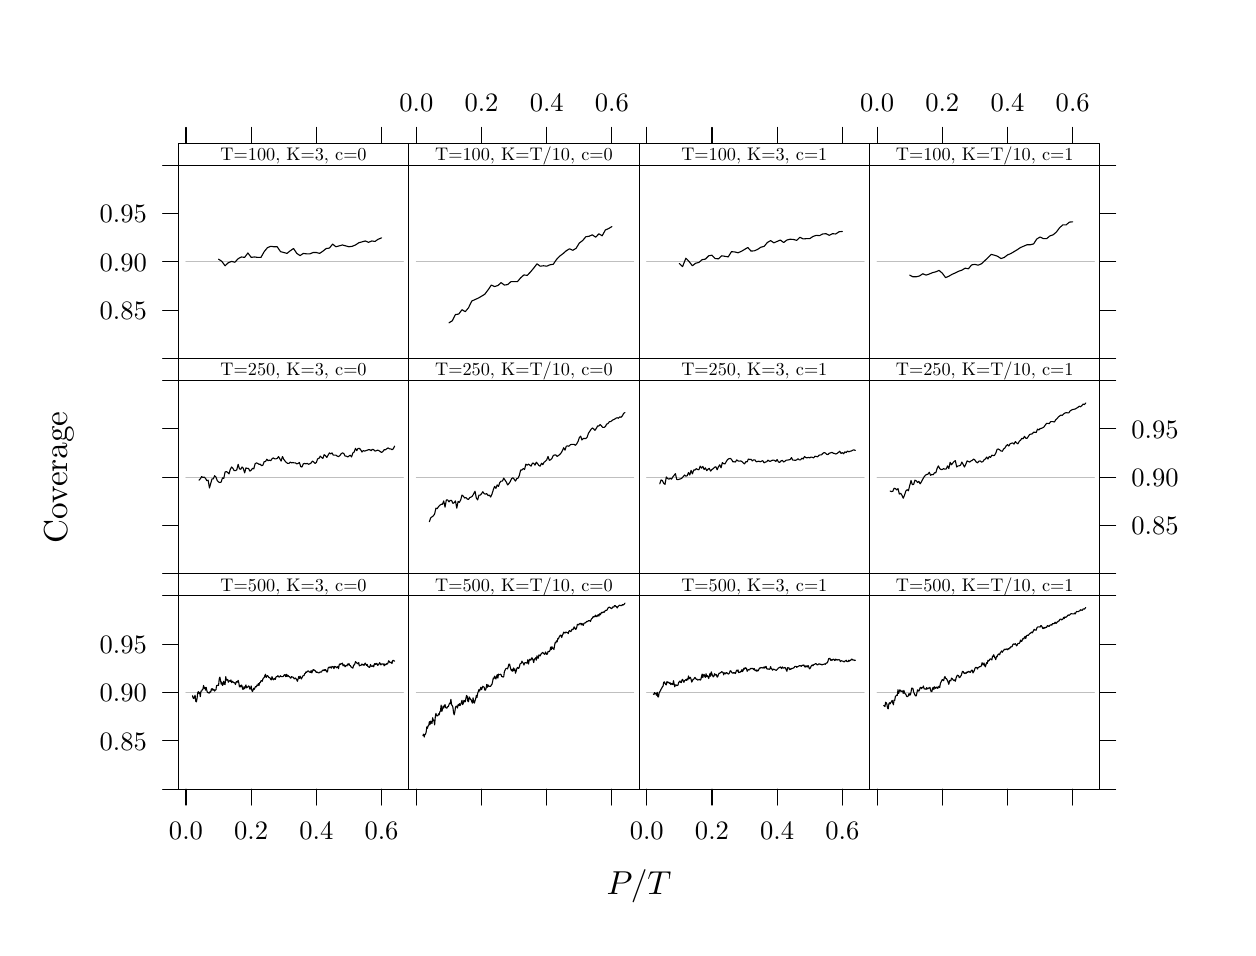
\begin{tikzpicture}[x=1pt,y=1pt]
\definecolor[named]{fillColor}{rgb}{1.00,1.00,1.00}
\path[use as bounding box,fill=fillColor,fill opacity=0.00] (0,0) rectangle (433.62,325.21);
\begin{scope}
\path[clip] (  0.00,  0.00) rectangle (433.62,325.21);

\path[] (  0.00,  0.00) rectangle (433.62,325.21);
\definecolor[named]{drawColor}{rgb}{0.00,0.00,0.00}

\node[text=drawColor,anchor=base,inner sep=0pt, outer sep=0pt, scale=  1.20] at (220.94, 12.05) {$P/T$};
\end{scope}
\begin{scope}
\path[clip] (  0.00,  0.00) rectangle (433.62,325.21);
\definecolor[named]{drawColor}{rgb}{0.00,0.00,0.00}

\node[text=drawColor,rotate= 90.00,anchor=base,inner sep=0pt, outer sep=0pt, scale=  1.20] at ( 14.29,162.76) {Coverage};
\end{scope}
\begin{scope}
\path[clip] (  0.00,  0.00) rectangle (433.62,325.21);
\definecolor[named]{drawColor}{rgb}{0.00,0.00,0.00}

\path[draw=drawColor,line width= 0.4pt,line join=round,line cap=round] ( 54.44, 50.02) -- ( 48.75, 50.02);

\path[draw=drawColor,line width= 0.4pt,line join=round,line cap=round] ( 54.44, 67.48) -- ( 48.75, 67.48);

\path[draw=drawColor,line width= 0.4pt,line join=round,line cap=round] ( 54.44, 84.95) -- ( 48.75, 84.95);

\path[draw=drawColor,line width= 0.4pt,line join=round,line cap=round] ( 54.44,102.42) -- ( 48.75,102.42);

\path[draw=drawColor,line width= 0.4pt,line join=round,line cap=round] ( 54.44,119.88) -- ( 48.75,119.88);

\node[text=drawColor,anchor=base east,inner sep=0pt, outer sep=0pt, scale=  0.96] at ( 43.06, 64.18) {0.85};

\node[text=drawColor,anchor=base east,inner sep=0pt, outer sep=0pt, scale=  0.96] at ( 43.06, 81.64) {0.90};

\node[text=drawColor,anchor=base east,inner sep=0pt, outer sep=0pt, scale=  0.96] at ( 43.06, 99.11) {0.95};
\end{scope}
\begin{scope}
\path[clip] (  0.00,  0.00) rectangle (433.62,325.21);
\definecolor[named]{drawColor}{rgb}{0.00,0.00,0.00}

\path[draw=drawColor,line width= 0.4pt,line join=round,line cap=round] ( 57.20, 50.02) -- ( 57.20, 44.32);

\path[draw=drawColor,line width= 0.4pt,line join=round,line cap=round] ( 80.76, 50.02) -- ( 80.76, 44.32);

\path[draw=drawColor,line width= 0.4pt,line join=round,line cap=round] (104.31, 50.02) -- (104.31, 44.32);

\path[draw=drawColor,line width= 0.4pt,line join=round,line cap=round] (127.87, 50.02) -- (127.87, 44.32);

\node[text=drawColor,anchor=base,inner sep=0pt, outer sep=0pt, scale=  0.96] at ( 57.20, 32.02) {0.0};

\node[text=drawColor,anchor=base,inner sep=0pt, outer sep=0pt, scale=  0.96] at ( 80.76, 32.02) {0.2};

\node[text=drawColor,anchor=base,inner sep=0pt, outer sep=0pt, scale=  0.96] at (104.31, 32.02) {0.4};

\node[text=drawColor,anchor=base,inner sep=0pt, outer sep=0pt, scale=  0.96] at (127.87, 32.02) {0.6};
\end{scope}
\begin{scope}
\path[clip] ( 54.44, 50.02) rectangle (137.69,119.88);
\definecolor[named]{drawColor}{rgb}{0.75,0.75,0.75}

\path[draw=drawColor,line width= 0.4pt,line join=round,line cap=round] ( 57.20, 84.95) --
	(135.72, 84.95);
\definecolor[named]{drawColor}{rgb}{0.00,0.00,0.00}

\path[draw=drawColor,line width= 0.4pt,line join=round,line cap=round] ( 59.56, 83.80) --
	( 59.79, 82.96) --
	( 60.03, 82.79) --
	( 60.26, 83.47) --
	( 60.50, 83.97) --
	( 60.73, 81.78) --
	( 60.97, 81.61) --
	( 61.20, 82.79) --
	( 61.44, 84.81) --
	( 61.68, 85.32) --
	( 61.91, 84.65) --
	( 62.15, 84.98) --
	( 62.38, 83.47) --
	( 62.62, 85.49) --
	( 62.85, 85.49) --
	( 63.09, 85.99) --
	( 63.32, 86.16) --
	( 63.56, 87.51) --
	( 63.80, 86.50) --
	( 64.03, 86.84) --
	( 64.27, 85.83) --
	( 64.50, 86.84) --
	( 64.74, 85.66) --
	( 64.97, 84.98) --
	( 65.21, 84.98) --
	( 65.44, 84.81) --
	( 65.68, 84.81) --
	( 65.92, 85.32) --
	( 66.15, 85.15) --
	( 66.39, 86.33) --
	( 66.62, 85.83) --
	( 66.86, 86.33) --
	( 67.09, 85.83) --
	( 67.33, 85.99) --
	( 67.56, 85.49) --
	( 67.80, 85.83) --
	( 68.04, 85.99) --
	( 68.27, 87.51) --
	( 68.51, 87.51) --
	( 68.74, 87.68) --
	( 68.98, 87.51) --
	( 69.21, 89.87) --
	( 69.45, 90.55) --
	( 69.69, 89.37) --
	( 69.92, 88.02) --
	( 70.16, 88.69) --
	( 70.39, 87.51) --
	( 70.63, 87.85) --
	( 70.86, 89.03) --
	( 71.10, 88.02) --
	( 71.33, 87.85) --
	( 71.57, 90.71) --
	( 71.81, 89.53) --
	( 72.04, 89.37) --
	( 72.28, 89.70) --
	( 72.51, 88.69) --
	( 72.75, 89.20) --
	( 72.98, 89.20) --
	( 73.22, 89.03) --
	( 73.45, 89.53) --
	( 73.69, 88.52) --
	( 73.93, 89.03) --
	( 74.16, 88.86) --
	( 74.40, 88.52) --
	( 74.63, 88.52) --
	( 74.87, 88.35) --
	( 75.10, 87.85) --
	( 75.34, 88.86) --
	( 75.57, 88.86) --
	( 75.81, 88.69) --
	( 76.05, 89.37) --
	( 76.28, 88.52) --
	( 76.52, 87.01) --
	( 76.75, 87.51) --
	( 76.99, 87.01) --
	( 77.22, 87.68) --
	( 77.46, 87.34) --
	( 77.69, 86.16) --
	( 77.93, 86.16) --
	( 78.17, 87.01) --
	( 78.40, 86.33) --
	( 78.64, 87.17) --
	( 78.87, 87.68) --
	( 79.11, 86.67) --
	( 79.34, 86.84) --
	( 79.58, 87.01) --
	( 79.81, 87.34) --
	( 80.05, 87.17) --
	( 80.29, 86.16) --
	( 80.52, 86.33) --
	( 80.76, 87.34) --
	( 80.99, 85.83) --
	( 81.23, 85.32) --
	( 81.46, 85.83) --
	( 81.70, 86.50) --
	( 81.93, 86.16) --
	( 82.17, 86.84) --
	( 82.41, 87.17) --
	( 82.64, 87.01) --
	( 82.88, 87.68) --
	( 83.11, 87.51) --
	( 83.35, 88.19) --
	( 83.58, 87.51) --
	( 83.82, 88.52) --
	( 84.05, 88.52) --
	( 84.29, 89.20) --
	( 84.53, 89.20) --
	( 84.76, 89.03) --
	( 85.00, 89.87) --
	( 85.23, 90.21) --
	( 85.47, 90.38) --
	( 85.70, 91.05) --
	( 85.94, 91.56) --
	( 86.17, 90.38) --
	( 86.41, 90.88) --
	( 86.65, 91.05) --
	( 86.88, 90.88) --
	( 87.12, 90.38) --
	( 87.35, 90.38) --
	( 87.59, 90.21) --
	( 87.82, 89.70) --
	( 88.06, 89.53) --
	( 88.29, 90.71) --
	( 88.53, 90.04) --
	( 88.77, 89.53) --
	( 89.00, 89.87) --
	( 89.24, 90.04) --
	( 89.47, 89.70) --
	( 89.71, 90.55) --
	( 89.94, 90.71) --
	( 90.18, 90.71) --
	( 90.41, 91.05) --
	( 90.65, 90.71) --
	( 90.89, 90.55) --
	( 91.12, 90.71) --
	( 91.36, 91.05) --
	( 91.59, 90.71) --
	( 91.83, 90.71) --
	( 92.06, 90.71) --
	( 92.30, 90.71) --
	( 92.53, 91.05) --
	( 92.77, 91.39) --
	( 93.01, 91.39) --
	( 93.24, 90.71) --
	( 93.48, 91.56) --
	( 93.71, 90.71) --
	( 93.95, 91.22) --
	( 94.18, 91.05) --
	( 94.42, 90.71) --
	( 94.66, 90.71) --
	( 94.89, 90.21) --
	( 95.13, 90.21) --
	( 95.36, 90.71) --
	( 95.60, 90.55) --
	( 95.83, 90.55) --
	( 96.07, 90.38) --
	( 96.30, 89.87) --
	( 96.54, 90.04) --
	( 96.78, 90.21) --
	( 97.01, 89.87) --
	( 97.25, 89.53) --
	( 97.48, 89.03) --
	( 97.72, 89.87) --
	( 97.95, 90.71) --
	( 98.19, 90.04) --
	( 98.42, 90.88) --
	( 98.66, 90.38) --
	( 98.90, 89.87) --
	( 99.13, 90.38) --
	( 99.37, 90.88) --
	( 99.60, 91.05) --
	( 99.84, 91.05) --
	(100.07, 91.73) --
	(100.31, 91.89) --
	(100.54, 92.40) --
	(100.78, 92.23) --
	(101.02, 92.57) --
	(101.25, 92.74) --
	(101.49, 92.74) --
	(101.72, 92.40) --
	(101.96, 92.40) --
	(102.19, 92.23) --
	(102.43, 92.91) --
	(102.66, 92.06) --
	(102.90, 92.57) --
	(103.14, 93.24) --
	(103.37, 93.24) --
	(103.61, 92.91) --
	(103.84, 92.91) --
	(104.08, 92.57) --
	(104.31, 92.23) --
	(104.55, 92.40) --
	(104.78, 92.23) --
	(105.02, 92.06) --
	(105.26, 92.06) --
	(105.49, 92.23) --
	(105.73, 92.40) --
	(105.96, 92.40) --
	(106.20, 92.40) --
	(106.43, 92.91) --
	(106.67, 93.08) --
	(106.90, 92.91) --
	(107.14, 93.24) --
	(107.38, 92.91) --
	(107.61, 93.24) --
	(107.85, 92.91) --
	(108.08, 92.40) --
	(108.32, 92.40) --
	(108.55, 93.75) --
	(108.79, 94.09) --
	(109.02, 93.92) --
	(109.26, 94.26) --
	(109.50, 94.09) --
	(109.73, 93.75) --
	(109.97, 94.42) --
	(110.20, 94.26) --
	(110.44, 94.26) --
	(110.67, 93.58) --
	(110.91, 94.42) --
	(111.14, 94.26) --
	(111.38, 94.26) --
	(111.62, 93.92) --
	(111.85, 94.09) --
	(112.09, 94.42) --
	(112.32, 93.58) --
	(112.56, 94.93) --
	(112.79, 95.27) --
	(113.03, 95.10) --
	(113.26, 95.44) --
	(113.50, 95.27) --
	(113.74, 95.60) --
	(113.97, 94.59) --
	(114.21, 94.93) --
	(114.44, 94.93) --
	(114.68, 94.26) --
	(114.91, 94.59) --
	(115.15, 94.76) --
	(115.38, 94.59) --
	(115.62, 95.27) --
	(115.86, 94.93) --
	(116.09, 95.44) --
	(116.33, 94.76) --
	(116.56, 94.76) --
	(116.80, 94.26) --
	(117.03, 94.09) --
	(117.27, 93.92) --
	(117.51, 93.75) --
	(117.74, 94.76) --
	(117.98, 94.93) --
	(118.21, 95.27) --
	(118.45, 96.11) --
	(118.68, 95.94) --
	(118.92, 95.60) --
	(119.15, 95.60) --
	(119.39, 95.27) --
	(119.63, 95.77) --
	(119.86, 94.59) --
	(120.10, 94.76) --
	(120.33, 94.76) --
	(120.57, 94.93) --
	(120.80, 95.27) --
	(121.04, 94.93) --
	(121.27, 95.10) --
	(121.51, 94.76) --
	(121.75, 95.27) --
	(121.98, 95.60) --
	(122.22, 95.10) --
	(122.45, 94.76) --
	(122.69, 95.10) --
	(122.92, 94.42) --
	(123.16, 94.26) --
	(123.39, 94.09) --
	(123.63, 94.09) --
	(123.87, 95.10) --
	(124.10, 94.59) --
	(124.34, 94.42) --
	(124.57, 94.42) --
	(124.81, 94.76) --
	(125.04, 94.26) --
	(125.28, 95.27) --
	(125.51, 95.44) --
	(125.75, 95.10) --
	(125.99, 95.44) --
	(126.22, 95.44) --
	(126.46, 94.76) --
	(126.69, 94.93) --
	(126.93, 95.27) --
	(127.16, 95.77) --
	(127.40, 95.44) --
	(127.63, 94.93) --
	(127.87, 95.27) --
	(128.11, 95.27) --
	(128.34, 95.27) --
	(128.58, 95.27) --
	(128.81, 94.59) --
	(129.05, 95.27) --
	(129.28, 94.93) --
	(129.52, 95.10) --
	(129.75, 95.44) --
	(129.99, 95.27) --
	(130.23, 95.77) --
	(130.46, 96.45) --
	(130.70, 96.11) --
	(130.93, 95.77) --
	(131.17, 95.77) --
	(131.40, 95.94) --
	(131.64, 95.44) --
	(131.87, 96.45) --
	(132.11, 96.62) --
	(132.35, 96.45) --
	(132.58, 96.28);
\end{scope}
\begin{scope}
\path[clip] (  0.00,  0.00) rectangle (433.62,325.21);
\definecolor[named]{drawColor}{rgb}{0.00,0.00,0.00}

\path[draw=drawColor,line width= 0.4pt,line join=round,line cap=round] ( 54.44, 50.02) rectangle (137.69,119.88);
\end{scope}
\begin{scope}
\path[clip] ( 54.44,119.88) rectangle (137.69,127.83);

\path[] ( 54.44,119.88) rectangle (137.69,127.83);
\definecolor[named]{drawColor}{rgb}{0.00,0.00,0.00}

\node[text=drawColor,anchor=base west,inner sep=0pt, outer sep=0pt, scale=  0.66] at ( 69.67,121.58) {T=500, K=3, c=0};
\end{scope}
\begin{scope}
\path[clip] (  0.00,  0.00) rectangle (433.62,325.21);
\definecolor[named]{drawColor}{rgb}{0.00,0.00,0.00}

\path[draw=drawColor,line width= 0.4pt,line join=round,line cap=round] ( 54.44,119.88) rectangle (137.69,127.83);
\end{scope}
\begin{scope}
\path[clip] (  0.00,  0.00) rectangle (433.62,325.21);
\definecolor[named]{drawColor}{rgb}{0.00,0.00,0.00}

\path[draw=drawColor,line width= 0.4pt,line join=round,line cap=round] (140.45, 50.02) -- (140.45, 44.32);

\path[draw=drawColor,line width= 0.4pt,line join=round,line cap=round] (164.01, 50.02) -- (164.01, 44.32);

\path[draw=drawColor,line width= 0.4pt,line join=round,line cap=round] (187.56, 50.02) -- (187.56, 44.32);

\path[draw=drawColor,line width= 0.4pt,line join=round,line cap=round] (211.12, 50.02) -- (211.12, 44.32);
\end{scope}
\begin{scope}
\path[clip] (137.69, 50.02) rectangle (220.94,119.88);
\definecolor[named]{drawColor}{rgb}{0.75,0.75,0.75}

\path[draw=drawColor,line width= 0.4pt,line join=round,line cap=round] (140.45, 84.95) --
	(218.97, 84.95);
\definecolor[named]{drawColor}{rgb}{0.00,0.00,0.00}

\path[draw=drawColor,line width= 0.4pt,line join=round,line cap=round] (142.80, 69.40) --
	(143.04, 69.93) --
	(143.28, 68.88) --
	(143.51, 69.75) --
	(143.75, 69.93) --
	(143.98, 70.63) --
	(144.22, 72.55) --
	(144.45, 72.02) --
	(144.69, 72.90) --
	(144.92, 73.07) --
	(145.16, 74.47) --
	(145.40, 73.42) --
	(145.63, 74.64) --
	(145.87, 74.12) --
	(146.10, 73.77) --
	(146.34, 75.87) --
	(146.57, 74.82) --
	(146.81, 74.99) --
	(147.05, 73.25) --
	(147.28, 76.04) --
	(147.52, 77.44) --
	(147.75, 76.56) --
	(147.99, 76.56) --
	(148.22, 76.56) --
	(148.46, 77.26) --
	(148.69, 76.91) --
	(148.93, 77.96) --
	(149.17, 78.31) --
	(149.40, 80.41) --
	(149.64, 78.14) --
	(149.87, 78.84) --
	(150.11, 80.06) --
	(150.34, 79.36) --
	(150.58, 80.23) --
	(150.81, 80.58) --
	(151.05, 79.53) --
	(151.29, 79.36) --
	(151.52, 79.36) --
	(151.76, 79.88) --
	(151.99, 79.88) --
	(152.23, 80.58) --
	(152.46, 81.11) --
	(152.70, 80.93) --
	(152.93, 82.50) --
	(153.17, 80.58) --
	(153.41, 80.23) --
	(153.64, 79.71) --
	(153.88, 77.79) --
	(154.11, 76.91) --
	(154.35, 77.96) --
	(154.58, 79.53) --
	(154.82, 80.06) --
	(155.05, 80.06) --
	(155.29, 79.36) --
	(155.53, 80.58) --
	(155.76, 80.23) --
	(156.00, 80.93) --
	(156.23, 80.23) --
	(156.47, 80.76) --
	(156.70, 81.28) --
	(156.94, 82.15) --
	(157.17, 80.58) --
	(157.41, 81.11) --
	(157.65, 82.15) --
	(157.88, 81.63) --
	(158.12, 81.63) --
	(158.35, 82.85) --
	(158.59, 83.90) --
	(158.82, 83.55) --
	(159.06, 81.80) --
	(159.29, 81.63) --
	(159.53, 83.38) --
	(159.77, 83.03) --
	(160.00, 82.50) --
	(160.24, 82.33) --
	(160.47, 81.63) --
	(160.71, 81.11) --
	(160.94, 83.03) --
	(161.18, 81.63) --
	(161.41, 81.11) --
	(161.65, 81.98) --
	(161.89, 82.68) --
	(162.12, 83.90) --
	(162.36, 83.20) --
	(162.59, 84.60) --
	(162.83, 85.30) --
	(163.06, 86.00) --
	(163.30, 85.47) --
	(163.53, 86.17) --
	(163.77, 86.87) --
	(164.01, 86.00) --
	(164.24, 86.70) --
	(164.48, 87.22) --
	(164.71, 87.04) --
	(164.95, 86.87) --
	(165.18, 85.82) --
	(165.42, 85.82) --
	(165.65, 86.52) --
	(165.89, 87.92) --
	(166.13, 86.87) --
	(166.36, 87.74) --
	(166.60, 87.22) --
	(166.83, 87.22) --
	(167.07, 87.22) --
	(167.30, 87.22) --
	(167.54, 87.74) --
	(167.77, 87.92) --
	(168.01, 88.97) --
	(168.25, 90.19) --
	(168.48, 90.01) --
	(168.72, 90.89) --
	(168.95, 90.36) --
	(169.19, 89.84) --
	(169.42, 90.71) --
	(169.66, 91.41) --
	(169.90, 90.19) --
	(170.13, 91.59) --
	(170.37, 91.41) --
	(170.60, 91.41) --
	(170.84, 91.59) --
	(171.07, 91.41) --
	(171.31, 90.71) --
	(171.54, 90.71) --
	(171.78, 90.54) --
	(172.02, 90.71) --
	(172.25, 92.46) --
	(172.49, 92.98) --
	(172.72, 93.51) --
	(172.96, 93.68) --
	(173.19, 93.68) --
	(173.43, 93.51) --
	(173.66, 94.38) --
	(173.90, 95.25) --
	(174.14, 95.25) --
	(174.37, 94.21) --
	(174.61, 93.33) --
	(174.84, 92.81) --
	(175.08, 93.33) --
	(175.31, 92.63) --
	(175.55, 93.86) --
	(175.78, 92.98) --
	(176.02, 93.51) --
	(176.26, 91.94) --
	(176.49, 92.63) --
	(176.73, 93.51) --
	(176.96, 94.03) --
	(177.20, 93.86) --
	(177.43, 93.68) --
	(177.67, 94.21) --
	(177.90, 95.25) --
	(178.14, 95.43) --
	(178.38, 95.60) --
	(178.61, 96.30) --
	(178.85, 95.78) --
	(179.08, 95.60) --
	(179.32, 94.90) --
	(179.55, 95.60) --
	(179.79, 95.78) --
	(180.02, 95.78) --
	(180.26, 95.60) --
	(180.50, 95.60) --
	(180.73, 96.83) --
	(180.97, 95.25) --
	(181.20, 96.48) --
	(181.44, 97.00) --
	(181.67, 96.65) --
	(181.91, 96.83) --
	(182.14, 97.52) --
	(182.38, 97.35) --
	(182.62, 96.65) --
	(182.85, 95.78) --
	(183.09, 97.00) --
	(183.32, 97.18) --
	(183.56, 97.52) --
	(183.79, 96.65) --
	(184.03, 98.22) --
	(184.26, 97.52) --
	(184.50, 97.35) --
	(184.74, 98.57) --
	(184.97, 98.40) --
	(185.21, 98.22) --
	(185.44, 98.75) --
	(185.68, 99.10) --
	(185.91, 99.27) --
	(186.15, 99.45) --
	(186.38, 99.10) --
	(186.62, 98.92) --
	(186.86, 98.75) --
	(187.09, 99.62) --
	(187.33, 99.27) --
	(187.56, 98.75) --
	(187.80, 98.92) --
	(188.03, 99.80) --
	(188.27, 99.80) --
	(188.50, 99.80) --
	(188.74,100.14) --
	(188.98,101.37) --
	(189.21,100.49) --
	(189.45,101.54) --
	(189.68,100.84) --
	(189.92,101.02) --
	(190.15,100.49) --
	(190.39,101.89) --
	(190.62,103.11) --
	(190.86,102.94) --
	(191.10,103.64) --
	(191.33,103.29) --
	(191.57,104.51) --
	(191.80,104.34) --
	(192.04,105.04) --
	(192.27,105.38) --
	(192.51,105.73) --
	(192.74,105.56) --
	(192.98,104.86) --
	(193.22,105.73) --
	(193.45,106.08) --
	(193.69,106.78) --
	(193.92,106.61) --
	(194.16,106.43) --
	(194.39,106.78) --
	(194.63,106.78) --
	(194.87,106.61) --
	(195.10,106.61) --
	(195.34,106.26) --
	(195.57,107.13) --
	(195.81,107.31) --
	(196.04,107.13) --
	(196.28,106.96) --
	(196.51,107.48) --
	(196.75,107.83) --
	(196.99,107.66) --
	(197.22,108.00) --
	(197.46,108.70) --
	(197.69,108.35) --
	(197.93,107.83) --
	(198.16,107.83) --
	(198.40,108.53) --
	(198.63,109.58) --
	(198.87,109.58) --
	(199.11,109.40) --
	(199.34,109.75) --
	(199.58,109.93) --
	(199.81,109.93) --
	(200.05,109.40) --
	(200.28,109.93) --
	(200.52,109.58) --
	(200.75,109.23) --
	(200.99,109.93) --
	(201.23,110.10) --
	(201.46,110.10) --
	(201.70,110.28) --
	(201.93,110.62) --
	(202.17,110.62) --
	(202.40,110.62) --
	(202.64,110.97) --
	(202.87,110.97) --
	(203.11,110.97) --
	(203.35,110.62) --
	(203.58,111.32) --
	(203.82,111.67) --
	(204.05,111.85) --
	(204.29,112.37) --
	(204.52,112.20) --
	(204.76,112.55) --
	(204.99,112.37) --
	(205.23,112.90) --
	(205.47,112.37) --
	(205.70,112.37) --
	(205.94,112.90) --
	(206.17,113.07) --
	(206.41,112.55) --
	(206.64,113.42) --
	(206.88,113.07) --
	(207.11,113.42) --
	(207.35,113.94) --
	(207.59,113.77) --
	(207.82,113.94) --
	(208.06,114.12) --
	(208.29,113.94) --
	(208.53,114.29) --
	(208.76,114.64) --
	(209.00,114.64) --
	(209.23,114.64) --
	(209.47,114.99) --
	(209.71,115.52) --
	(209.94,115.69) --
	(210.18,115.86) --
	(210.41,115.69) --
	(210.65,115.52) --
	(210.88,115.34) --
	(211.12,115.34) --
	(211.35,115.86) --
	(211.59,115.86) --
	(211.83,115.86) --
	(212.06,116.39) --
	(212.30,116.39) --
	(212.53,116.04) --
	(212.77,116.04) --
	(213.00,115.52) --
	(213.24,115.86) --
	(213.47,116.21) --
	(213.71,116.39) --
	(213.95,116.56) --
	(214.18,116.39) --
	(214.42,116.39) --
	(214.65,116.39) --
	(214.89,116.74) --
	(215.12,116.56) --
	(215.36,116.74) --
	(215.59,116.91) --
	(215.83,117.26);
\end{scope}
\begin{scope}
\path[clip] (  0.00,  0.00) rectangle (433.62,325.21);
\definecolor[named]{drawColor}{rgb}{0.00,0.00,0.00}

\path[draw=drawColor,line width= 0.4pt,line join=round,line cap=round] (137.69, 50.02) rectangle (220.94,119.88);
\end{scope}
\begin{scope}
\path[clip] (137.69,119.88) rectangle (220.94,127.83);

\path[] (137.69,119.88) rectangle (220.94,127.83);
\definecolor[named]{drawColor}{rgb}{0.00,0.00,0.00}

\node[text=drawColor,anchor=base west,inner sep=0pt, outer sep=0pt, scale=  0.66] at (147.24,121.58) {T=500, K=T/10, c=0};
\end{scope}
\begin{scope}
\path[clip] (  0.00,  0.00) rectangle (433.62,325.21);
\definecolor[named]{drawColor}{rgb}{0.00,0.00,0.00}

\path[draw=drawColor,line width= 0.4pt,line join=round,line cap=round] (137.69,119.88) rectangle (220.94,127.83);
\end{scope}
\begin{scope}
\path[clip] (  0.00,  0.00) rectangle (433.62,325.21);
\definecolor[named]{drawColor}{rgb}{0.00,0.00,0.00}

\path[draw=drawColor,line width= 0.4pt,line join=round,line cap=round] (223.70, 50.02) -- (223.70, 44.32);

\path[draw=drawColor,line width= 0.4pt,line join=round,line cap=round] (247.26, 50.02) -- (247.26, 44.32);

\path[draw=drawColor,line width= 0.4pt,line join=round,line cap=round] (270.81, 50.02) -- (270.81, 44.32);

\path[draw=drawColor,line width= 0.4pt,line join=round,line cap=round] (294.37, 50.02) -- (294.37, 44.32);

\node[text=drawColor,anchor=base,inner sep=0pt, outer sep=0pt, scale=  0.96] at (223.70, 32.02) {0.0};

\node[text=drawColor,anchor=base,inner sep=0pt, outer sep=0pt, scale=  0.96] at (247.26, 32.02) {0.2};

\node[text=drawColor,anchor=base,inner sep=0pt, outer sep=0pt, scale=  0.96] at (270.81, 32.02) {0.4};

\node[text=drawColor,anchor=base,inner sep=0pt, outer sep=0pt, scale=  0.96] at (294.37, 32.02) {0.6};
\end{scope}
\begin{scope}
\path[clip] (220.94, 50.02) rectangle (304.19,119.88);
\definecolor[named]{drawColor}{rgb}{0.75,0.75,0.75}

\path[draw=drawColor,line width= 0.4pt,line join=round,line cap=round] (223.70, 84.95) --
	(302.22, 84.95);
\definecolor[named]{drawColor}{rgb}{0.00,0.00,0.00}

\path[draw=drawColor,line width= 0.4pt,line join=round,line cap=round] (226.05, 84.45) --
	(226.29, 84.25) --
	(226.53, 84.95) --
	(226.76, 84.55) --
	(227.00, 84.65) --
	(227.23, 83.95) --
	(227.47, 85.05) --
	(227.70, 83.45) --
	(227.94, 83.35) --
	(228.17, 84.85) --
	(228.41, 85.25) --
	(228.65, 85.65) --
	(228.88, 86.15) --
	(229.12, 86.55) --
	(229.35, 87.04) --
	(229.59, 87.24) --
	(229.82, 88.64) --
	(230.06, 88.84) --
	(230.29, 88.34) --
	(230.53, 87.84) --
	(230.77, 87.74) --
	(231.00, 88.94) --
	(231.24, 88.54) --
	(231.47, 88.74) --
	(231.71, 88.54) --
	(231.94, 88.24) --
	(232.18, 88.44) --
	(232.41, 87.84) --
	(232.65, 88.24) --
	(232.89, 88.04) --
	(233.12, 87.84) --
	(233.36, 89.24) --
	(233.59, 88.14) --
	(233.83, 87.04) --
	(234.06, 87.74) --
	(234.30, 87.74) --
	(234.53, 87.44) --
	(234.77, 87.54) --
	(235.01, 87.64) --
	(235.24, 88.74) --
	(235.48, 88.74) --
	(235.71, 89.14) --
	(235.95, 88.64) --
	(236.18, 88.54) --
	(236.42, 89.44) --
	(236.65, 89.74) --
	(236.89, 89.14) --
	(237.13, 88.64) --
	(237.36, 89.24) --
	(237.60, 89.44) --
	(237.83, 89.64) --
	(238.07, 89.34) --
	(238.30, 89.94) --
	(238.54, 89.54) --
	(238.77, 90.94) --
	(239.01, 89.94) --
	(239.25, 90.34) --
	(239.48, 90.44) --
	(239.72, 89.74) --
	(239.95, 88.74) --
	(240.19, 89.14) --
	(240.42, 89.74) --
	(240.66, 89.74) --
	(240.89, 90.14) --
	(241.13, 90.44) --
	(241.37, 90.04) --
	(241.60, 89.74) --
	(241.84, 89.84) --
	(242.07, 89.44) --
	(242.31, 89.54) --
	(242.54, 89.64) --
	(242.78, 89.74) --
	(243.01, 89.44) --
	(243.25, 89.64) --
	(243.49, 90.74) --
	(243.72, 91.64) --
	(243.96, 90.34) --
	(244.19, 91.24) --
	(244.43, 91.54) --
	(244.66, 90.74) --
	(244.90, 90.44) --
	(245.13, 91.74) --
	(245.37, 90.74) --
	(245.61, 91.04) --
	(245.84, 90.64) --
	(246.08, 90.04) --
	(246.31, 90.94) --
	(246.55, 91.84) --
	(246.78, 90.84) --
	(247.02, 92.43) --
	(247.26, 91.64) --
	(247.49, 91.04) --
	(247.73, 90.64) --
	(247.96, 90.84) --
	(248.20, 91.74) --
	(248.43, 91.24) --
	(248.67, 91.54) --
	(248.90, 91.34) --
	(249.14, 90.54) --
	(249.38, 90.74) --
	(249.61, 91.44) --
	(249.85, 91.94) --
	(250.08, 91.94) --
	(250.32, 92.14) --
	(250.55, 92.23) --
	(250.79, 92.53) --
	(251.02, 92.33) --
	(251.26, 92.23) --
	(251.50, 91.34) --
	(251.73, 92.04) --
	(251.97, 92.04) --
	(252.20, 91.74) --
	(252.44, 92.14) --
	(252.67, 92.14) --
	(252.91, 91.84) --
	(253.14, 91.64) --
	(253.38, 91.74) --
	(253.62, 92.14) --
	(253.85, 92.83) --
	(254.09, 92.73) --
	(254.32, 92.43) --
	(254.56, 92.04) --
	(254.79, 91.94) --
	(255.03, 92.14) --
	(255.26, 91.94) --
	(255.50, 92.14) --
	(255.74, 91.84) --
	(255.97, 92.53) --
	(256.21, 93.03) --
	(256.44, 92.73) --
	(256.68, 93.13) --
	(256.91, 92.14) --
	(257.15, 92.33) --
	(257.38, 92.23) --
	(257.62, 92.63) --
	(257.86, 92.53) --
	(258.09, 93.23) --
	(258.33, 92.53) --
	(258.56, 93.03) --
	(258.80, 93.73) --
	(259.03, 93.43) --
	(259.27, 93.93) --
	(259.50, 93.73) --
	(259.74, 93.73) --
	(259.98, 92.63) --
	(260.21, 93.03) --
	(260.45, 93.23) --
	(260.68, 93.13) --
	(260.92, 93.23) --
	(261.15, 93.63) --
	(261.39, 93.73) --
	(261.62, 93.53) --
	(261.86, 93.73) --
	(262.10, 93.63) --
	(262.33, 93.23) --
	(262.57, 93.63) --
	(262.80, 92.93) --
	(263.04, 92.83) --
	(263.27, 93.13) --
	(263.51, 92.63) --
	(263.74, 93.03) --
	(263.98, 92.83) --
	(264.22, 93.33) --
	(264.45, 93.83) --
	(264.69, 93.73) --
	(264.92, 94.03) --
	(265.16, 93.93) --
	(265.39, 93.83) --
	(265.63, 93.93) --
	(265.86, 94.13) --
	(266.10, 93.73) --
	(266.34, 94.23) --
	(266.57, 93.93) --
	(266.81, 94.43) --
	(267.04, 93.63) --
	(267.28, 93.43) --
	(267.51, 93.53) --
	(267.75, 93.43) --
	(267.98, 93.33) --
	(268.22, 93.53) --
	(268.46, 94.33) --
	(268.69, 93.63) --
	(268.93, 93.43) --
	(269.16, 93.03) --
	(269.40, 93.43) --
	(269.63, 93.33) --
	(269.87, 93.33) --
	(270.11, 93.13) --
	(270.34, 93.03) --
	(270.58, 93.03) --
	(270.81, 93.33) --
	(271.05, 93.53) --
	(271.28, 93.83) --
	(271.52, 93.93) --
	(271.75, 94.03) --
	(271.99, 94.23) --
	(272.23, 93.83) --
	(272.46, 93.63) --
	(272.70, 94.23) --
	(272.93, 93.93) --
	(273.17, 93.73) --
	(273.40, 93.93) --
	(273.64, 94.03) --
	(273.87, 93.73) --
	(274.11, 93.13) --
	(274.35, 92.63) --
	(274.58, 93.93) --
	(274.82, 93.83) --
	(275.05, 93.93) --
	(275.29, 93.23) --
	(275.52, 93.53) --
	(275.76, 93.33) --
	(275.99, 93.63) --
	(276.23, 93.63) --
	(276.47, 93.73) --
	(276.70, 93.83) --
	(276.94, 93.93) --
	(277.17, 94.33) --
	(277.41, 94.43) --
	(277.64, 94.43) --
	(277.88, 94.03) --
	(278.11, 94.33) --
	(278.35, 94.33) --
	(278.59, 94.53) --
	(278.82, 94.63) --
	(279.06, 94.63) --
	(279.29, 94.63) --
	(279.53, 94.43) --
	(279.76, 94.73) --
	(280.00, 94.83) --
	(280.23, 94.73) --
	(280.47, 94.93) --
	(280.71, 94.43) --
	(280.94, 94.13) --
	(281.18, 94.63) --
	(281.41, 94.53) --
	(281.65, 94.13) --
	(281.88, 94.63) --
	(282.12, 94.63) --
	(282.35, 93.83) --
	(282.59, 93.53) --
	(282.83, 93.83) --
	(283.06, 94.43) --
	(283.30, 94.73) --
	(283.53, 94.93) --
	(283.77, 94.63) --
	(284.00, 95.03) --
	(284.24, 95.13) --
	(284.47, 95.23) --
	(284.71, 95.43) --
	(284.95, 95.33) --
	(285.18, 95.03) --
	(285.42, 94.93) --
	(285.65, 95.13) --
	(285.89, 95.33) --
	(286.12, 95.33) --
	(286.36, 95.13) --
	(286.59, 95.23) --
	(286.83, 95.03) --
	(287.07, 94.93) --
	(287.30, 95.13) --
	(287.54, 95.13) --
	(287.77, 95.23) --
	(288.01, 95.33) --
	(288.24, 95.13) --
	(288.48, 95.53) --
	(288.71, 95.63) --
	(288.95, 95.73) --
	(289.19, 96.33) --
	(289.42, 97.13) --
	(289.66, 97.33) --
	(289.89, 97.33) --
	(290.13, 96.63) --
	(290.36, 96.83) --
	(290.60, 96.53) --
	(290.83, 96.93) --
	(291.07, 96.93) --
	(291.31, 97.03) --
	(291.54, 96.53) --
	(291.78, 96.63) --
	(292.01, 97.03) --
	(292.25, 96.83) --
	(292.48, 96.63) --
	(292.72, 96.83) --
	(292.96, 96.73) --
	(293.19, 96.83) --
	(293.43, 96.73) --
	(293.66, 96.13) --
	(293.90, 96.43) --
	(294.13, 96.43) --
	(294.37, 96.33) --
	(294.60, 96.33) --
	(294.84, 96.13) --
	(295.08, 96.03) --
	(295.31, 96.33) --
	(295.55, 96.43) --
	(295.78, 96.63) --
	(296.02, 96.13) --
	(296.25, 96.23) --
	(296.49, 96.13) --
	(296.72, 96.63) --
	(296.96, 96.33) --
	(297.20, 96.53) --
	(297.43, 96.63) --
	(297.67, 97.03) --
	(297.90, 97.03) --
	(298.14, 96.73) --
	(298.37, 96.73) --
	(298.61, 96.73) --
	(298.84, 96.53) --
	(299.08, 96.63);
\end{scope}
\begin{scope}
\path[clip] (  0.00,  0.00) rectangle (433.62,325.21);
\definecolor[named]{drawColor}{rgb}{0.00,0.00,0.00}

\path[draw=drawColor,line width= 0.4pt,line join=round,line cap=round] (220.94, 50.02) rectangle (304.19,119.88);
\end{scope}
\begin{scope}
\path[clip] (220.94,119.88) rectangle (304.19,127.83);

\path[] (220.94,119.88) rectangle (304.19,127.83);
\definecolor[named]{drawColor}{rgb}{0.00,0.00,0.00}

\node[text=drawColor,anchor=base west,inner sep=0pt, outer sep=0pt, scale=  0.66] at (236.17,121.58) {T=500, K=3, c=1};
\end{scope}
\begin{scope}
\path[clip] (  0.00,  0.00) rectangle (433.62,325.21);
\definecolor[named]{drawColor}{rgb}{0.00,0.00,0.00}

\path[draw=drawColor,line width= 0.4pt,line join=round,line cap=round] (220.94,119.88) rectangle (304.19,127.83);
\end{scope}
\begin{scope}
\path[clip] (  0.00,  0.00) rectangle (433.62,325.21);
\definecolor[named]{drawColor}{rgb}{0.00,0.00,0.00}

\path[draw=drawColor,line width= 0.4pt,line join=round,line cap=round] (306.95, 50.02) -- (306.95, 44.32);

\path[draw=drawColor,line width= 0.4pt,line join=round,line cap=round] (330.50, 50.02) -- (330.50, 44.32);

\path[draw=drawColor,line width= 0.4pt,line join=round,line cap=round] (354.06, 50.02) -- (354.06, 44.32);

\path[draw=drawColor,line width= 0.4pt,line join=round,line cap=round] (377.62, 50.02) -- (377.62, 44.32);

\path[draw=drawColor,line width= 0.4pt,line join=round,line cap=round] (387.44, 50.02) -- (393.13, 50.02);

\path[draw=drawColor,line width= 0.4pt,line join=round,line cap=round] (387.44, 67.48) -- (393.13, 67.48);

\path[draw=drawColor,line width= 0.4pt,line join=round,line cap=round] (387.44, 84.95) -- (393.13, 84.95);

\path[draw=drawColor,line width= 0.4pt,line join=round,line cap=round] (387.44,102.42) -- (393.13,102.42);

\path[draw=drawColor,line width= 0.4pt,line join=round,line cap=round] (387.44,119.88) -- (393.13,119.88);
\end{scope}
\begin{scope}
\path[clip] (304.19, 50.02) rectangle (387.44,119.88);
\definecolor[named]{drawColor}{rgb}{0.75,0.75,0.75}

\path[draw=drawColor,line width= 0.4pt,line join=round,line cap=round] (306.95, 84.95) --
	(385.47, 84.95);
\definecolor[named]{drawColor}{rgb}{0.00,0.00,0.00}

\path[draw=drawColor,line width= 0.4pt,line join=round,line cap=round] (309.30, 80.26) --
	(309.54, 80.16) --
	(309.77, 79.86) --
	(310.01, 81.46) --
	(310.25, 81.26) --
	(310.48, 80.76) --
	(310.72, 79.36) --
	(310.95, 79.06) --
	(311.19, 80.86) --
	(311.42, 81.26) --
	(311.66, 80.86) --
	(311.89, 81.36) --
	(312.13, 81.66) --
	(312.37, 82.15) --
	(312.60, 81.16) --
	(312.84, 80.56) --
	(313.07, 82.25) --
	(313.31, 82.15) --
	(313.54, 83.55) --
	(313.78, 83.75) --
	(314.01, 84.05) --
	(314.25, 83.95) --
	(314.49, 85.95) --
	(314.72, 84.65) --
	(314.96, 85.45) --
	(315.19, 85.95) --
	(315.43, 85.55) --
	(315.66, 85.35) --
	(315.90, 85.55) --
	(316.13, 85.55) --
	(316.37, 84.65) --
	(316.61, 85.75) --
	(316.84, 84.95) --
	(317.08, 84.45) --
	(317.31, 84.45) --
	(317.55, 83.65) --
	(317.78, 83.45) --
	(318.02, 83.55) --
	(318.25, 83.85) --
	(318.49, 84.65) --
	(318.73, 84.05) --
	(318.96, 84.15) --
	(319.20, 85.15) --
	(319.43, 86.55) --
	(319.67, 86.55) --
	(319.90, 86.35) --
	(320.14, 85.15) --
	(320.37, 84.65) --
	(320.61, 84.05) --
	(320.85, 83.75) --
	(321.08, 83.75) --
	(321.32, 84.85) --
	(321.55, 85.95) --
	(321.79, 85.75) --
	(322.02, 85.45) --
	(322.26, 85.95) --
	(322.50, 86.75) --
	(322.73, 86.85) --
	(322.97, 86.35) --
	(323.20, 86.75) --
	(323.44, 86.75) --
	(323.67, 87.34) --
	(323.91, 86.35) --
	(324.14, 86.25) --
	(324.38, 86.25) --
	(324.62, 86.15) --
	(324.85, 86.75) --
	(325.09, 86.25) --
	(325.32, 86.35) --
	(325.56, 86.65) --
	(325.79, 86.55) --
	(326.03, 86.85) --
	(326.26, 85.85) --
	(326.50, 85.25) --
	(326.74, 85.35) --
	(326.97, 86.45) --
	(327.21, 86.85) --
	(327.44, 86.05) --
	(327.68, 87.04) --
	(327.91, 86.75) --
	(328.15, 86.45) --
	(328.38, 86.94) --
	(328.62, 86.94) --
	(328.86, 86.45) --
	(329.09, 86.94) --
	(329.33, 87.24) --
	(329.56, 86.75) --
	(329.80, 88.24) --
	(330.03, 88.74) --
	(330.27, 89.24) --
	(330.50, 89.64) --
	(330.74, 89.44) --
	(330.98, 89.24) --
	(331.21, 90.24) --
	(331.45, 90.74) --
	(331.68, 90.14) --
	(331.92, 90.04) --
	(332.15, 89.74) --
	(332.39, 89.24) --
	(332.62, 88.64) --
	(332.86, 87.94) --
	(333.10, 89.14) --
	(333.33, 89.34) --
	(333.57, 89.14) --
	(333.80, 90.14) --
	(334.04, 90.04) --
	(334.27, 89.74) --
	(334.51, 89.44) --
	(334.74, 89.24) --
	(334.98, 89.54) --
	(335.22, 89.04) --
	(335.45, 90.14) --
	(335.69, 90.74) --
	(335.92, 91.24) --
	(336.16, 91.14) --
	(336.39, 91.04) --
	(336.63, 90.34) --
	(336.86, 90.44) --
	(337.10, 90.84) --
	(337.34, 91.14) --
	(337.57, 91.94) --
	(337.81, 92.63) --
	(338.04, 92.53) --
	(338.28, 92.04) --
	(338.51, 91.84) --
	(338.75, 92.14) --
	(338.98, 91.84) --
	(339.22, 92.04) --
	(339.46, 92.43) --
	(339.69, 92.23) --
	(339.93, 92.63) --
	(340.16, 92.53) --
	(340.40, 92.33) --
	(340.63, 92.23) --
	(340.87, 92.73) --
	(341.10, 93.03) --
	(341.34, 93.03) --
	(341.58, 92.04) --
	(341.81, 92.43) --
	(342.05, 92.93) --
	(342.28, 93.63) --
	(342.52, 94.03) --
	(342.75, 94.03) --
	(342.99, 93.93) --
	(343.22, 93.43) --
	(343.46, 94.03) --
	(343.70, 94.03) --
	(343.93, 94.33) --
	(344.17, 94.33) --
	(344.40, 94.33) --
	(344.64, 94.73) --
	(344.87, 95.73) --
	(345.11, 95.23) --
	(345.35, 94.93) --
	(345.58, 95.63) --
	(345.82, 94.73) --
	(346.05, 94.23) --
	(346.29, 95.03) --
	(346.52, 95.73) --
	(346.76, 95.53) --
	(346.99, 96.63) --
	(347.23, 96.33) --
	(347.47, 96.63) --
	(347.70, 97.03) --
	(347.94, 97.13) --
	(348.17, 96.93) --
	(348.41, 96.73) --
	(348.64, 98.12) --
	(348.88, 98.02) --
	(349.11, 98.62) --
	(349.35, 97.72) --
	(349.59, 97.42) --
	(349.82, 96.83) --
	(350.06, 98.02) --
	(350.29, 97.82) --
	(350.53, 98.52) --
	(350.76, 98.82) --
	(351.00, 98.92) --
	(351.23, 98.62) --
	(351.47, 99.42) --
	(351.71, 99.62) --
	(351.94,100.02) --
	(352.18, 99.52) --
	(352.41, 99.92) --
	(352.65,100.12) --
	(352.88,100.62) --
	(353.12,100.52) --
	(353.35,100.52) --
	(353.59,100.72) --
	(353.83,100.62) --
	(354.06,100.42) --
	(354.30,100.82) --
	(354.53,100.62) --
	(354.77,101.12) --
	(355.00,101.02) --
	(355.24,101.52) --
	(355.47,101.42) --
	(355.71,101.52) --
	(355.95,102.22) --
	(356.18,102.52) --
	(356.42,102.42) --
	(356.65,102.42) --
	(356.89,102.62) --
	(357.12,102.22) --
	(357.36,101.82) --
	(357.59,102.22) --
	(357.83,102.71) --
	(358.07,102.71) --
	(358.30,102.71) --
	(358.54,103.11) --
	(358.77,103.91) --
	(359.01,103.41) --
	(359.24,103.51) --
	(359.48,104.21) --
	(359.71,104.51) --
	(359.95,104.31) --
	(360.19,104.91) --
	(360.42,105.21) --
	(360.66,104.51) --
	(360.89,105.41) --
	(361.13,105.61) --
	(361.36,105.71) --
	(361.60,105.61) --
	(361.83,106.01) --
	(362.07,106.21) --
	(362.31,106.41) --
	(362.54,106.61) --
	(362.78,106.81) --
	(363.01,106.51) --
	(363.25,106.91) --
	(363.48,107.41) --
	(363.72,107.81) --
	(363.95,107.51) --
	(364.19,107.61) --
	(364.43,107.51) --
	(364.66,108.30) --
	(364.90,108.60) --
	(365.13,108.70) --
	(365.37,108.70) --
	(365.60,108.70) --
	(365.84,108.60) --
	(366.07,109.10) --
	(366.31,109.10) --
	(366.55,108.70) --
	(366.78,108.10) --
	(367.02,108.10) --
	(367.25,108.50) --
	(367.49,108.20) --
	(367.72,108.40) --
	(367.96,108.60) --
	(368.19,108.50) --
	(368.43,109.10) --
	(368.67,109.10) --
	(368.90,108.90) --
	(369.14,108.90) --
	(369.37,109.30) --
	(369.61,109.30) --
	(369.84,109.50) --
	(370.08,109.30) --
	(370.32,109.90) --
	(370.55,109.80) --
	(370.79,109.90) --
	(371.02,109.90) --
	(371.26,110.40) --
	(371.49,110.00) --
	(371.73,110.00) --
	(371.96,110.40) --
	(372.20,110.50) --
	(372.44,110.80) --
	(372.67,110.80) --
	(372.91,111.30) --
	(373.14,111.50) --
	(373.38,111.50) --
	(373.61,111.20) --
	(373.85,111.40) --
	(374.08,111.50) --
	(374.32,112.10) --
	(374.56,111.70) --
	(374.79,112.30) --
	(375.03,112.10) --
	(375.26,112.20) --
	(375.50,112.40) --
	(375.73,112.70) --
	(375.97,113.00) --
	(376.20,112.90) --
	(376.44,112.90) --
	(376.68,113.19) --
	(376.91,113.39) --
	(377.15,113.49) --
	(377.38,113.39) --
	(377.62,113.39) --
	(377.85,113.39) --
	(378.09,113.39) --
	(378.32,113.69) --
	(378.56,113.39) --
	(378.80,113.89) --
	(379.03,114.29) --
	(379.27,114.19) --
	(379.50,114.19) --
	(379.74,114.19) --
	(379.97,114.49) --
	(380.21,114.49) --
	(380.44,114.89) --
	(380.68,114.69) --
	(380.92,114.79) --
	(381.15,114.69) --
	(381.39,115.19) --
	(381.62,115.19) --
	(381.86,115.09) --
	(382.09,115.39) --
	(382.33,115.69);
\end{scope}
\begin{scope}
\path[clip] (  0.00,  0.00) rectangle (433.62,325.21);
\definecolor[named]{drawColor}{rgb}{0.00,0.00,0.00}

\path[draw=drawColor,line width= 0.4pt,line join=round,line cap=round] (304.19, 50.02) rectangle (387.44,119.88);
\end{scope}
\begin{scope}
\path[clip] (304.19,119.88) rectangle (387.44,127.83);

\path[] (304.19,119.88) rectangle (387.44,127.83);
\definecolor[named]{drawColor}{rgb}{0.00,0.00,0.00}

\node[text=drawColor,anchor=base west,inner sep=0pt, outer sep=0pt, scale=  0.66] at (313.74,121.58) {T=500, K=T/10, c=1};
\end{scope}
\begin{scope}
\path[clip] (  0.00,  0.00) rectangle (433.62,325.21);
\definecolor[named]{drawColor}{rgb}{0.00,0.00,0.00}

\path[draw=drawColor,line width= 0.4pt,line join=round,line cap=round] (304.19,119.88) rectangle (387.44,127.83);
\end{scope}
\begin{scope}
\path[clip] (  0.00,  0.00) rectangle (433.62,325.21);
\definecolor[named]{drawColor}{rgb}{0.00,0.00,0.00}

\path[draw=drawColor,line width= 0.4pt,line join=round,line cap=round] ( 54.44,127.83) -- ( 48.75,127.83);

\path[draw=drawColor,line width= 0.4pt,line join=round,line cap=round] ( 54.44,145.30) -- ( 48.75,145.30);

\path[draw=drawColor,line width= 0.4pt,line join=round,line cap=round] ( 54.44,162.76) -- ( 48.75,162.76);

\path[draw=drawColor,line width= 0.4pt,line join=round,line cap=round] ( 54.44,180.23) -- ( 48.75,180.23);

\path[draw=drawColor,line width= 0.4pt,line join=round,line cap=round] ( 54.44,197.70) -- ( 48.75,197.70);
\end{scope}
\begin{scope}
\path[clip] ( 54.44,127.83) rectangle (137.69,197.70);
\definecolor[named]{drawColor}{rgb}{0.75,0.75,0.75}

\path[draw=drawColor,line width= 0.4pt,line join=round,line cap=round] ( 57.20,162.76) --
	(135.72,162.76);
\definecolor[named]{drawColor}{rgb}{0.00,0.00,0.00}

\path[draw=drawColor,line width= 0.4pt,line join=round,line cap=round] ( 61.91,161.68) --
	( 62.38,162.17) --
	( 62.85,163.00) --
	( 63.32,162.67) --
	( 63.80,162.83) --
	( 64.27,162.34) --
	( 64.74,161.51) --
	( 65.21,161.68) --
	( 65.68,158.88) --
	( 66.15,160.53) --
	( 66.62,162.17) --
	( 67.09,162.17) --
	( 67.56,163.32) --
	( 68.04,162.83) --
	( 68.51,161.51) --
	( 68.98,161.02) --
	( 69.45,160.86) --
	( 69.92,161.02) --
	( 70.39,162.50) --
	( 70.86,162.34) --
	( 71.33,164.64) --
	( 71.81,164.80) --
	( 72.28,164.48) --
	( 72.75,163.98) --
	( 73.22,165.63) --
	( 73.69,166.45) --
	( 74.16,165.96) --
	( 74.63,165.13) --
	( 75.10,165.13) --
	( 75.57,165.46) --
	( 76.05,167.44) --
	( 76.52,165.79) --
	( 76.99,165.63) --
	( 77.46,166.45) --
	( 77.93,165.96) --
	( 78.40,164.31) --
	( 78.87,166.12) --
	( 79.34,165.96) --
	( 79.81,165.96) --
	( 80.29,164.97) --
	( 80.76,165.30) --
	( 81.23,165.96) --
	( 81.70,165.79) --
	( 82.17,167.60) --
	( 82.64,167.93) --
	( 83.11,167.76) --
	( 83.58,167.44) --
	( 84.05,167.44) --
	( 84.53,166.94) --
	( 85.00,167.11) --
	( 85.47,168.42) --
	( 85.94,168.42) --
	( 86.41,169.25) --
	( 86.88,168.75) --
	( 87.35,168.92) --
	( 87.82,168.75) --
	( 88.29,169.41) --
	( 88.77,169.74) --
	( 89.24,169.41) --
	( 89.71,169.41) --
	( 90.18,169.57) --
	( 90.65,170.23) --
	( 91.12,169.41) --
	( 91.59,168.59) --
	( 92.06,170.23) --
	( 92.53,169.25) --
	( 93.01,168.59) --
	( 93.48,168.09) --
	( 93.95,167.76) --
	( 94.42,167.76) --
	( 94.89,168.26) --
	( 95.36,167.93) --
	( 95.83,168.09) --
	( 96.30,167.93) --
	( 96.78,167.93) --
	( 97.25,167.60) --
	( 97.72,167.76) --
	( 98.19,168.09) --
	( 98.66,166.61) --
	( 99.13,166.45) --
	( 99.60,167.60) --
	(100.07,167.76) --
	(100.54,167.60) --
	(101.02,167.76) --
	(101.49,167.44) --
	(101.96,167.60) --
	(102.43,167.93) --
	(102.90,168.59) --
	(103.37,168.26) --
	(103.84,167.76) --
	(104.31,168.09) --
	(104.78,169.41) --
	(105.26,169.57) --
	(105.73,170.40) --
	(106.20,169.90) --
	(106.67,169.57) --
	(107.14,170.89) --
	(107.61,170.56) --
	(108.08,169.90) --
	(108.55,170.73) --
	(109.02,171.55) --
	(109.50,171.22) --
	(109.97,171.55) --
	(110.44,170.73) --
	(110.91,170.73) --
	(111.38,170.73) --
	(111.85,170.40) --
	(112.32,170.23) --
	(112.79,170.56) --
	(113.26,171.22) --
	(113.74,171.55) --
	(114.21,171.38) --
	(114.68,170.40) --
	(115.15,170.40) --
	(115.62,170.07) --
	(116.09,170.40) --
	(116.56,170.73) --
	(117.03,170.07) --
	(117.51,171.55) --
	(117.98,171.88) --
	(118.45,173.19) --
	(118.92,172.37) --
	(119.39,173.19) --
	(119.86,173.19) --
	(120.33,172.70) --
	(120.80,171.88) --
	(121.27,172.37) --
	(121.75,172.21) --
	(122.22,172.37) --
	(122.69,172.53) --
	(123.16,172.70) --
	(123.63,172.70) --
	(124.10,172.37) --
	(124.57,172.86) --
	(125.04,172.70) --
	(125.51,172.21) --
	(125.99,172.37) --
	(126.46,172.53) --
	(126.93,172.37) --
	(127.40,172.04) --
	(127.87,171.71) --
	(128.34,172.04) --
	(128.81,172.70) --
	(129.28,172.70) --
	(129.75,173.03) --
	(130.23,173.36) --
	(130.70,173.03) --
	(131.17,173.03) --
	(131.64,172.70) --
	(132.11,173.03) --
	(132.58,174.01);
\end{scope}
\begin{scope}
\path[clip] (  0.00,  0.00) rectangle (433.62,325.21);
\definecolor[named]{drawColor}{rgb}{0.00,0.00,0.00}

\path[draw=drawColor,line width= 0.4pt,line join=round,line cap=round] ( 54.44,127.83) rectangle (137.69,197.70);
\end{scope}
\begin{scope}
\path[clip] ( 54.44,197.70) rectangle (137.69,205.65);

\path[] ( 54.44,197.70) rectangle (137.69,205.65);
\definecolor[named]{drawColor}{rgb}{0.00,0.00,0.00}

\node[text=drawColor,anchor=base west,inner sep=0pt, outer sep=0pt, scale=  0.66] at ( 69.67,199.40) {T=250, K=3, c=0};
\end{scope}
\begin{scope}
\path[clip] (  0.00,  0.00) rectangle (433.62,325.21);
\definecolor[named]{drawColor}{rgb}{0.00,0.00,0.00}

\path[draw=drawColor,line width= 0.4pt,line join=round,line cap=round] ( 54.44,197.70) rectangle (137.69,205.65);
\end{scope}
\begin{scope}
\path[clip] (137.69,127.83) rectangle (220.94,197.70);
\definecolor[named]{drawColor}{rgb}{0.75,0.75,0.75}

\path[draw=drawColor,line width= 0.4pt,line join=round,line cap=round] (140.45,162.76) --
	(218.97,162.76);
\definecolor[named]{drawColor}{rgb}{0.00,0.00,0.00}

\path[draw=drawColor,line width= 0.4pt,line join=round,line cap=round] (145.16,146.70) --
	(145.63,148.09) --
	(146.10,148.44) --
	(146.57,148.79) --
	(147.05,149.49) --
	(147.52,151.59) --
	(147.99,151.41) --
	(148.46,152.11) --
	(148.93,152.63) --
	(149.40,152.98) --
	(149.87,152.98) --
	(150.34,154.21) --
	(150.81,151.94) --
	(151.29,154.56) --
	(151.76,154.56) --
	(152.23,153.86) --
	(152.70,154.38) --
	(153.17,154.38) --
	(153.64,153.33) --
	(154.11,153.51) --
	(154.58,154.21) --
	(155.05,151.59) --
	(155.53,154.03) --
	(156.00,153.68) --
	(156.47,154.56) --
	(156.94,156.30) --
	(157.41,155.95) --
	(157.88,155.25) --
	(158.35,155.43) --
	(158.82,154.90) --
	(159.29,154.73) --
	(159.77,155.43) --
	(160.24,155.60) --
	(160.71,155.95) --
	(161.18,156.83) --
	(161.65,157.70) --
	(162.12,155.25) --
	(162.59,154.56) --
	(163.06,156.30) --
	(163.53,156.30) --
	(164.01,156.83) --
	(164.48,157.52) --
	(164.95,156.83) --
	(165.42,156.65) --
	(165.89,156.83) --
	(166.36,156.13) --
	(166.83,156.30) --
	(167.30,155.60) --
	(167.77,156.65) --
	(168.25,158.22) --
	(168.72,159.45) --
	(169.19,158.75) --
	(169.66,159.97) --
	(170.13,159.45) --
	(170.60,160.84) --
	(171.07,161.37) --
	(171.54,161.37) --
	(172.02,162.42) --
	(172.49,161.72) --
	(172.96,161.02) --
	(173.43,159.97) --
	(173.90,160.49) --
	(174.37,161.19) --
	(174.84,162.24) --
	(175.31,162.59) --
	(175.78,162.07) --
	(176.26,161.37) --
	(176.73,162.24) --
	(177.20,162.42) --
	(177.67,163.46) --
	(178.14,165.38) --
	(178.61,165.38) --
	(179.08,165.91) --
	(179.55,165.56) --
	(180.02,167.48) --
	(180.50,167.13) --
	(180.97,167.48) --
	(181.44,167.13) --
	(181.91,166.78) --
	(182.38,167.83) --
	(182.85,167.83) --
	(183.32,167.13) --
	(183.79,168.18) --
	(184.26,167.66) --
	(184.74,166.96) --
	(185.21,166.78) --
	(185.68,167.83) --
	(186.15,167.31) --
	(186.62,168.18) --
	(187.09,168.53) --
	(187.56,169.05) --
	(188.03,170.28) --
	(188.50,168.88) --
	(188.98,169.05) --
	(189.45,169.58) --
	(189.92,170.62) --
	(190.39,170.80) --
	(190.86,170.80) --
	(191.33,170.28) --
	(191.80,170.62) --
	(192.27,170.97) --
	(192.74,171.50) --
	(193.22,172.37) --
	(193.69,173.42) --
	(194.16,172.55) --
	(194.63,173.94) --
	(195.10,174.12) --
	(195.57,173.94) --
	(196.04,174.47) --
	(196.51,174.64) --
	(196.99,174.64) --
	(197.46,174.64) --
	(197.93,174.29) --
	(198.40,174.82) --
	(198.87,175.69) --
	(199.34,177.09) --
	(199.81,177.61) --
	(200.28,176.21) --
	(200.75,176.74) --
	(201.23,176.74) --
	(201.70,176.74) --
	(202.17,177.26) --
	(202.64,178.66) --
	(203.11,179.36) --
	(203.58,180.06) --
	(204.05,180.58) --
	(204.52,180.23) --
	(204.99,179.71) --
	(205.47,180.41) --
	(205.94,181.28) --
	(206.41,181.28) --
	(206.88,181.80) --
	(207.35,181.28) --
	(207.82,180.76) --
	(208.29,180.76) --
	(208.76,181.10) --
	(209.23,181.98) --
	(209.71,182.15) --
	(210.18,182.85) --
	(210.65,182.85) --
	(211.12,183.20) --
	(211.59,183.55) --
	(212.06,183.72) --
	(212.53,184.07) --
	(213.00,184.25) --
	(213.47,184.07) --
	(213.95,184.60) --
	(214.42,184.42) --
	(214.89,184.95) --
	(215.36,185.82) --
	(215.83,186.17);
\end{scope}
\begin{scope}
\path[clip] (  0.00,  0.00) rectangle (433.62,325.21);
\definecolor[named]{drawColor}{rgb}{0.00,0.00,0.00}

\path[draw=drawColor,line width= 0.4pt,line join=round,line cap=round] (137.69,127.83) rectangle (220.94,197.70);
\end{scope}
\begin{scope}
\path[clip] (137.69,197.70) rectangle (220.94,205.65);

\path[] (137.69,197.70) rectangle (220.94,205.65);
\definecolor[named]{drawColor}{rgb}{0.00,0.00,0.00}

\node[text=drawColor,anchor=base west,inner sep=0pt, outer sep=0pt, scale=  0.66] at (147.24,199.40) {T=250, K=T/10, c=0};
\end{scope}
\begin{scope}
\path[clip] (  0.00,  0.00) rectangle (433.62,325.21);
\definecolor[named]{drawColor}{rgb}{0.00,0.00,0.00}

\path[draw=drawColor,line width= 0.4pt,line join=round,line cap=round] (137.69,197.70) rectangle (220.94,205.65);
\end{scope}
\begin{scope}
\path[clip] (220.94,127.83) rectangle (304.19,197.70);
\definecolor[named]{drawColor}{rgb}{0.75,0.75,0.75}

\path[draw=drawColor,line width= 0.4pt,line join=round,line cap=round] (223.70,162.76) --
	(302.22,162.76);
\definecolor[named]{drawColor}{rgb}{0.00,0.00,0.00}

\path[draw=drawColor,line width= 0.4pt,line join=round,line cap=round] (228.41,160.37) --
	(228.88,161.77) --
	(229.35,161.57) --
	(229.82,160.57) --
	(230.29,160.17) --
	(230.77,162.86) --
	(231.24,162.27) --
	(231.71,162.07) --
	(232.18,162.37) --
	(232.65,162.07) --
	(233.12,162.86) --
	(233.59,163.46) --
	(234.06,164.06) --
	(234.53,161.97) --
	(235.01,161.87) --
	(235.48,162.07) --
	(235.95,162.17) --
	(236.42,162.47) --
	(236.89,162.96) --
	(237.36,163.56) --
	(237.83,163.16) --
	(238.30,163.26) --
	(238.77,164.46) --
	(239.25,163.56) --
	(239.72,165.26) --
	(240.19,163.96) --
	(240.66,165.36) --
	(241.13,165.36) --
	(241.60,165.86) --
	(242.07,165.56) --
	(242.54,165.46) --
	(243.01,166.76) --
	(243.49,166.06) --
	(243.96,166.66) --
	(244.43,165.56) --
	(244.90,166.16) --
	(245.37,165.16) --
	(245.84,165.66) --
	(246.31,165.96) --
	(246.78,164.96) --
	(247.26,165.56) --
	(247.73,165.86) --
	(248.20,166.36) --
	(248.67,166.56) --
	(249.14,165.46) --
	(249.61,166.56) --
	(250.08,167.26) --
	(250.55,166.16) --
	(251.02,168.05) --
	(251.50,167.66) --
	(251.97,167.56) --
	(252.44,168.45) --
	(252.91,169.15) --
	(253.38,169.45) --
	(253.85,169.55) --
	(254.32,169.25) --
	(254.79,168.35) --
	(255.26,168.35) --
	(255.74,168.25) --
	(256.21,169.05) --
	(256.68,168.65) --
	(257.15,168.55) --
	(257.62,168.65) --
	(258.09,168.45) --
	(258.56,167.96) --
	(259.03,167.56) --
	(259.50,168.35) --
	(259.98,168.35) --
	(260.45,169.35) --
	(260.92,169.15) --
	(261.39,169.25) --
	(261.86,168.65) --
	(262.33,169.05) --
	(262.80,169.05) --
	(263.27,168.35) --
	(263.74,168.45) --
	(264.22,168.55) --
	(264.69,168.35) --
	(265.16,168.55) --
	(265.63,168.75) --
	(266.10,167.96) --
	(266.57,168.25) --
	(267.04,168.35) --
	(267.51,168.95) --
	(267.98,168.55) --
	(268.46,168.55) --
	(268.93,168.85) --
	(269.40,168.95) --
	(269.87,168.85) --
	(270.34,168.45) --
	(270.81,169.15) --
	(271.28,168.25) --
	(271.75,168.15) --
	(272.23,168.65) --
	(272.70,168.85) --
	(273.17,168.25) --
	(273.64,168.55) --
	(274.11,168.95) --
	(274.58,168.95) --
	(275.05,169.05) --
	(275.52,169.15) --
	(275.99,169.85) --
	(276.47,168.95) --
	(276.94,168.95) --
	(277.41,168.85) --
	(277.88,169.05) --
	(278.35,169.45) --
	(278.82,169.05) --
	(279.29,169.05) --
	(279.76,169.65) --
	(280.23,169.35) --
	(280.71,170.25) --
	(281.18,169.85) --
	(281.65,169.75) --
	(282.12,169.95) --
	(282.59,169.75) --
	(283.06,170.05) --
	(283.53,169.95) --
	(284.00,169.75) --
	(284.47,170.35) --
	(284.95,170.25) --
	(285.42,170.15) --
	(285.89,170.65) --
	(286.36,170.85) --
	(286.83,170.85) --
	(287.30,171.35) --
	(287.77,171.65) --
	(288.24,171.55) --
	(288.71,171.05) --
	(289.19,170.95) --
	(289.66,171.45) --
	(290.13,171.55) --
	(290.60,171.75) --
	(291.07,171.45) --
	(291.54,171.35) --
	(292.01,171.15) --
	(292.48,171.35) --
	(292.96,171.75) --
	(293.43,172.15) --
	(293.90,171.35) --
	(294.37,171.65) --
	(294.84,171.25) --
	(295.31,171.95) --
	(295.78,171.65) --
	(296.25,172.25) --
	(296.72,171.95) --
	(297.20,172.15) --
	(297.67,172.25) --
	(298.14,172.55) --
	(298.61,172.65) --
	(299.08,172.45);
\end{scope}
\begin{scope}
\path[clip] (  0.00,  0.00) rectangle (433.62,325.21);
\definecolor[named]{drawColor}{rgb}{0.00,0.00,0.00}

\path[draw=drawColor,line width= 0.4pt,line join=round,line cap=round] (220.94,127.83) rectangle (304.19,197.70);
\end{scope}
\begin{scope}
\path[clip] (220.94,197.70) rectangle (304.19,205.65);

\path[] (220.94,197.70) rectangle (304.19,205.65);
\definecolor[named]{drawColor}{rgb}{0.00,0.00,0.00}

\node[text=drawColor,anchor=base west,inner sep=0pt, outer sep=0pt, scale=  0.66] at (236.17,199.40) {T=250, K=3, c=1};
\end{scope}
\begin{scope}
\path[clip] (  0.00,  0.00) rectangle (433.62,325.21);
\definecolor[named]{drawColor}{rgb}{0.00,0.00,0.00}

\path[draw=drawColor,line width= 0.4pt,line join=round,line cap=round] (220.94,197.70) rectangle (304.19,205.65);
\end{scope}
\begin{scope}
\path[clip] (  0.00,  0.00) rectangle (433.62,325.21);
\definecolor[named]{drawColor}{rgb}{0.00,0.00,0.00}

\path[draw=drawColor,line width= 0.4pt,line join=round,line cap=round] (387.44,127.83) -- (393.13,127.83);

\path[draw=drawColor,line width= 0.4pt,line join=round,line cap=round] (387.44,145.30) -- (393.13,145.30);

\path[draw=drawColor,line width= 0.4pt,line join=round,line cap=round] (387.44,162.76) -- (393.13,162.76);

\path[draw=drawColor,line width= 0.4pt,line join=round,line cap=round] (387.44,180.23) -- (393.13,180.23);

\path[draw=drawColor,line width= 0.4pt,line join=round,line cap=round] (387.44,197.70) -- (393.13,197.70);

\node[text=drawColor,anchor=base west,inner sep=0pt, outer sep=0pt, scale=  0.96] at (398.82,141.99) {0.85};

\node[text=drawColor,anchor=base west,inner sep=0pt, outer sep=0pt, scale=  0.96] at (398.82,159.46) {0.90};

\node[text=drawColor,anchor=base west,inner sep=0pt, outer sep=0pt, scale=  0.96] at (398.82,176.93) {0.95};
\end{scope}
\begin{scope}
\path[clip] (304.19,127.83) rectangle (387.44,197.70);
\definecolor[named]{drawColor}{rgb}{0.75,0.75,0.75}

\path[draw=drawColor,line width= 0.4pt,line join=round,line cap=round] (306.95,162.76) --
	(385.47,162.76);
\definecolor[named]{drawColor}{rgb}{0.00,0.00,0.00}

\path[draw=drawColor,line width= 0.4pt,line join=round,line cap=round] (311.66,157.77) --
	(312.13,157.57) --
	(312.60,157.67) --
	(313.07,158.77) --
	(313.54,158.67) --
	(314.01,158.17) --
	(314.49,158.67) --
	(314.96,156.68) --
	(315.43,156.98) --
	(315.90,156.28) --
	(316.37,155.18) --
	(316.84,156.28) --
	(317.31,157.77) --
	(317.78,158.27) --
	(318.25,157.87) --
	(318.73,159.77) --
	(319.20,161.57) --
	(319.67,160.07) --
	(320.14,160.17) --
	(320.61,161.67) --
	(321.08,161.47) --
	(321.55,160.87) --
	(322.02,161.27) --
	(322.50,160.37) --
	(322.97,161.17) --
	(323.44,162.07) --
	(323.91,162.86) --
	(324.38,163.46) --
	(324.85,163.76) --
	(325.32,163.86) --
	(325.79,164.56) --
	(326.26,163.46) --
	(326.74,163.76) --
	(327.21,163.66) --
	(327.68,164.36) --
	(328.15,164.36) --
	(328.62,165.96) --
	(329.09,166.86) --
	(329.56,165.86) --
	(330.03,165.56) --
	(330.50,165.56) --
	(330.98,165.86) --
	(331.45,165.66) --
	(331.92,165.76) --
	(332.39,166.86) --
	(332.86,165.86) --
	(333.33,168.15) --
	(333.80,167.26) --
	(334.27,167.86) --
	(334.74,168.45) --
	(335.22,168.75) --
	(335.69,166.46) --
	(336.16,166.86) --
	(336.63,166.86) --
	(337.10,167.16) --
	(337.57,168.25) --
	(338.04,167.36) --
	(338.51,166.46) --
	(338.98,167.46) --
	(339.46,168.65) --
	(339.93,168.45) --
	(340.40,168.25) --
	(340.87,168.65) --
	(341.34,168.85) --
	(341.81,169.35) --
	(342.28,168.95) --
	(342.75,168.25) --
	(343.22,167.96) --
	(343.70,168.55) --
	(344.17,168.65) --
	(344.64,168.25) --
	(345.11,168.35) --
	(345.58,169.05) --
	(346.05,169.35) --
	(346.52,170.05) --
	(346.99,169.35) --
	(347.47,170.25) --
	(347.94,169.95) --
	(348.41,170.75) --
	(348.88,170.55) --
	(349.35,170.65) --
	(349.82,171.45) --
	(350.29,172.85) --
	(350.76,172.95) --
	(351.23,172.65) --
	(351.71,172.25) --
	(352.18,172.15) --
	(352.65,172.95) --
	(353.12,173.34) --
	(353.59,174.14) --
	(354.06,174.54) --
	(354.53,174.04) --
	(355.00,174.84) --
	(355.47,175.04) --
	(355.95,175.14) --
	(356.42,174.74) --
	(356.89,175.64) --
	(357.36,175.14) --
	(357.83,174.84) --
	(358.30,175.74) --
	(358.77,176.14) --
	(359.24,176.84) --
	(359.71,176.64) --
	(360.19,177.54) --
	(360.66,176.84) --
	(361.13,176.84) --
	(361.60,177.54) --
	(362.07,178.24) --
	(362.54,178.34) --
	(363.01,178.44) --
	(363.48,179.03) --
	(363.95,179.03) --
	(364.43,178.93) --
	(364.90,180.13) --
	(365.37,179.83) --
	(365.84,180.33) --
	(366.31,180.43) --
	(366.78,180.63) --
	(367.25,180.93) --
	(367.72,181.63) --
	(368.19,182.23) --
	(368.67,182.23) --
	(369.14,182.13) --
	(369.61,182.83) --
	(370.08,182.83) --
	(370.55,182.83) --
	(371.02,182.73) --
	(371.49,183.53) --
	(371.96,183.92) --
	(372.44,184.52) --
	(372.91,184.92) --
	(373.38,185.22) --
	(373.85,185.12) --
	(374.32,185.62) --
	(374.79,185.92) --
	(375.26,186.12) --
	(375.73,186.02) --
	(376.20,186.02) --
	(376.68,186.72) --
	(377.15,187.02) --
	(377.62,187.22) --
	(378.09,187.32) --
	(378.56,187.42) --
	(379.03,187.72) --
	(379.50,188.02) --
	(379.97,188.42) --
	(380.44,188.22) --
	(380.92,188.62) --
	(381.39,189.21) --
	(381.86,189.01) --
	(382.33,189.61);
\end{scope}
\begin{scope}
\path[clip] (  0.00,  0.00) rectangle (433.62,325.21);
\definecolor[named]{drawColor}{rgb}{0.00,0.00,0.00}

\path[draw=drawColor,line width= 0.4pt,line join=round,line cap=round] (304.19,127.83) rectangle (387.44,197.70);
\end{scope}
\begin{scope}
\path[clip] (304.19,197.70) rectangle (387.44,205.65);

\path[] (304.19,197.70) rectangle (387.44,205.65);
\definecolor[named]{drawColor}{rgb}{0.00,0.00,0.00}

\node[text=drawColor,anchor=base west,inner sep=0pt, outer sep=0pt, scale=  0.66] at (313.74,199.40) {T=250, K=T/10, c=1};
\end{scope}
\begin{scope}
\path[clip] (  0.00,  0.00) rectangle (433.62,325.21);
\definecolor[named]{drawColor}{rgb}{0.00,0.00,0.00}

\path[draw=drawColor,line width= 0.4pt,line join=round,line cap=round] (304.19,197.70) rectangle (387.44,205.65);
\end{scope}
\begin{scope}
\path[clip] (  0.00,  0.00) rectangle (433.62,325.21);
\definecolor[named]{drawColor}{rgb}{0.00,0.00,0.00}

\path[draw=drawColor,line width= 0.4pt,line join=round,line cap=round] ( 57.20,283.46) -- ( 57.20,289.15);

\path[draw=drawColor,line width= 0.4pt,line join=round,line cap=round] ( 80.76,283.46) -- ( 80.76,289.15);

\path[draw=drawColor,line width= 0.4pt,line join=round,line cap=round] (104.31,283.46) -- (104.31,289.15);

\path[draw=drawColor,line width= 0.4pt,line join=round,line cap=round] (127.87,283.46) -- (127.87,289.15);
\end{scope}
\begin{scope}
\path[clip] (  0.00,  0.00) rectangle (433.62,325.21);
\definecolor[named]{drawColor}{rgb}{0.00,0.00,0.00}

\path[draw=drawColor,line width= 0.4pt,line join=round,line cap=round] ( 54.44,205.65) -- ( 48.75,205.65);

\path[draw=drawColor,line width= 0.4pt,line join=round,line cap=round] ( 54.44,223.11) -- ( 48.75,223.11);

\path[draw=drawColor,line width= 0.4pt,line join=round,line cap=round] ( 54.44,240.58) -- ( 48.75,240.58);

\path[draw=drawColor,line width= 0.4pt,line join=round,line cap=round] ( 54.44,258.05) -- ( 48.75,258.05);

\path[draw=drawColor,line width= 0.4pt,line join=round,line cap=round] ( 54.44,275.51) -- ( 48.75,275.51);

\node[text=drawColor,anchor=base east,inner sep=0pt, outer sep=0pt, scale=  0.96] at ( 43.06,219.81) {0.85};

\node[text=drawColor,anchor=base east,inner sep=0pt, outer sep=0pt, scale=  0.96] at ( 43.06,237.28) {0.90};

\node[text=drawColor,anchor=base east,inner sep=0pt, outer sep=0pt, scale=  0.96] at ( 43.06,254.74) {0.95};
\end{scope}
\begin{scope}
\path[clip] ( 54.44,205.65) rectangle (137.69,275.51);
\definecolor[named]{drawColor}{rgb}{0.75,0.75,0.75}

\path[draw=drawColor,line width= 0.4pt,line join=round,line cap=round] ( 57.20,240.58) --
	(135.72,240.58);
\definecolor[named]{drawColor}{rgb}{0.00,0.00,0.00}

\path[draw=drawColor,line width= 0.4pt,line join=round,line cap=round] ( 68.98,241.56) --
	( 70.16,240.76) --
	( 71.33,239.16) --
	( 72.51,240.28) --
	( 73.69,240.76) --
	( 74.87,240.44) --
	( 76.05,241.72) --
	( 77.22,242.36) --
	( 78.40,242.20) --
	( 79.58,243.80) --
	( 80.76,242.20) --
	( 81.93,242.36) --
	( 83.11,242.20) --
	( 84.29,242.20) --
	( 85.47,244.28) --
	( 86.65,245.72) --
	( 87.82,246.20) --
	( 89.00,246.04) --
	( 90.18,246.04) --
	( 91.36,244.28) --
	( 92.53,243.96) --
	( 93.71,243.64) --
	( 94.89,244.60) --
	( 96.07,245.40) --
	( 97.25,243.64) --
	( 98.42,242.84) --
	( 99.60,243.64) --
	(100.78,243.48) --
	(101.96,243.48) --
	(103.14,243.96) --
	(104.31,243.96) --
	(105.49,243.64) --
	(106.67,244.44) --
	(107.85,245.40) --
	(109.02,245.56) --
	(110.20,247.00) --
	(111.38,246.04) --
	(112.56,246.36) --
	(113.74,246.68) --
	(114.91,246.36) --
	(116.09,246.04) --
	(117.27,246.20) --
	(118.45,246.68) --
	(119.63,247.48) --
	(120.80,247.80) --
	(121.98,248.13) --
	(123.16,247.64) --
	(124.34,248.13) --
	(125.51,247.97) --
	(126.69,248.77) --
	(127.87,249.25);
\end{scope}
\begin{scope}
\path[clip] (  0.00,  0.00) rectangle (433.62,325.21);
\definecolor[named]{drawColor}{rgb}{0.00,0.00,0.00}

\path[draw=drawColor,line width= 0.4pt,line join=round,line cap=round] ( 54.44,205.65) rectangle (137.69,275.51);
\end{scope}
\begin{scope}
\path[clip] ( 54.44,275.51) rectangle (137.69,283.46);

\path[] ( 54.44,275.51) rectangle (137.69,283.46);
\definecolor[named]{drawColor}{rgb}{0.00,0.00,0.00}

\node[text=drawColor,anchor=base west,inner sep=0pt, outer sep=0pt, scale=  0.66] at ( 69.67,277.22) {T=100, K=3, c=0};
\end{scope}
\begin{scope}
\path[clip] (  0.00,  0.00) rectangle (433.62,325.21);
\definecolor[named]{drawColor}{rgb}{0.00,0.00,0.00}

\path[draw=drawColor,line width= 0.4pt,line join=round,line cap=round] ( 54.44,275.51) rectangle (137.69,283.46);
\end{scope}
\begin{scope}
\path[clip] (  0.00,  0.00) rectangle (433.62,325.21);
\definecolor[named]{drawColor}{rgb}{0.00,0.00,0.00}

\path[draw=drawColor,line width= 0.4pt,line join=round,line cap=round] (140.45,283.46) -- (140.45,289.15);

\path[draw=drawColor,line width= 0.4pt,line join=round,line cap=round] (164.01,283.46) -- (164.01,289.15);

\path[draw=drawColor,line width= 0.4pt,line join=round,line cap=round] (187.56,283.46) -- (187.56,289.15);

\path[draw=drawColor,line width= 0.4pt,line join=round,line cap=round] (211.12,283.46) -- (211.12,289.15);

\node[text=drawColor,anchor=base,inner sep=0pt, outer sep=0pt, scale=  0.96] at (140.45,294.85) {0.0};

\node[text=drawColor,anchor=base,inner sep=0pt, outer sep=0pt, scale=  0.96] at (164.01,294.85) {0.2};

\node[text=drawColor,anchor=base,inner sep=0pt, outer sep=0pt, scale=  0.96] at (187.56,294.85) {0.4};

\node[text=drawColor,anchor=base,inner sep=0pt, outer sep=0pt, scale=  0.96] at (211.12,294.85) {0.6};
\end{scope}
\begin{scope}
\path[clip] (137.69,205.65) rectangle (220.94,275.51);
\definecolor[named]{drawColor}{rgb}{0.75,0.75,0.75}

\path[draw=drawColor,line width= 0.4pt,line join=round,line cap=round] (140.45,240.58) --
	(218.97,240.58);
\definecolor[named]{drawColor}{rgb}{0.00,0.00,0.00}

\path[draw=drawColor,line width= 0.4pt,line join=round,line cap=round] (152.23,218.57) --
	(153.41,219.27) --
	(154.58,221.54) --
	(155.76,221.72) --
	(156.94,223.29) --
	(158.12,222.59) --
	(159.29,223.99) --
	(160.47,226.43) --
	(161.65,226.96) --
	(162.83,227.48) --
	(164.01,228.18) --
	(165.18,228.88) --
	(166.36,230.45) --
	(167.54,232.20) --
	(168.72,231.67) --
	(169.90,232.02) --
	(171.07,233.07) --
	(172.25,232.20) --
	(173.43,232.37) --
	(174.61,233.42) --
	(175.78,233.42) --
	(176.96,233.42) --
	(178.14,234.82) --
	(179.32,235.87) --
	(180.50,235.69) --
	(181.67,236.91) --
	(182.85,238.31) --
	(184.03,239.88) --
	(185.21,239.01) --
	(186.38,239.18) --
	(187.56,239.01) --
	(188.74,239.53) --
	(189.92,239.71) --
	(191.10,241.45) --
	(192.27,242.68) --
	(193.45,243.55) --
	(194.63,244.60) --
	(195.81,245.30) --
	(196.99,244.77) --
	(198.16,245.47) --
	(199.34,247.39) --
	(200.52,248.27) --
	(201.70,249.66) --
	(202.87,249.84) --
	(204.05,250.36) --
	(205.23,249.49) --
	(206.41,250.71) --
	(207.59,250.01) --
	(208.76,252.11) --
	(209.94,252.63) --
	(211.12,253.33);
\end{scope}
\begin{scope}
\path[clip] (  0.00,  0.00) rectangle (433.62,325.21);
\definecolor[named]{drawColor}{rgb}{0.00,0.00,0.00}

\path[draw=drawColor,line width= 0.4pt,line join=round,line cap=round] (137.69,205.65) rectangle (220.94,275.51);
\end{scope}
\begin{scope}
\path[clip] (137.69,275.51) rectangle (220.94,283.46);

\path[] (137.69,275.51) rectangle (220.94,283.46);
\definecolor[named]{drawColor}{rgb}{0.00,0.00,0.00}

\node[text=drawColor,anchor=base west,inner sep=0pt, outer sep=0pt, scale=  0.66] at (147.24,277.22) {T=100, K=T/10, c=0};
\end{scope}
\begin{scope}
\path[clip] (  0.00,  0.00) rectangle (433.62,325.21);
\definecolor[named]{drawColor}{rgb}{0.00,0.00,0.00}

\path[draw=drawColor,line width= 0.4pt,line join=round,line cap=round] (137.69,275.51) rectangle (220.94,283.46);
\end{scope}
\begin{scope}
\path[clip] (  0.00,  0.00) rectangle (433.62,325.21);
\definecolor[named]{drawColor}{rgb}{0.00,0.00,0.00}

\path[draw=drawColor,line width= 0.4pt,line join=round,line cap=round] (223.70,283.46) -- (223.70,289.15);

\path[draw=drawColor,line width= 0.4pt,line join=round,line cap=round] (247.26,283.46) -- (247.26,289.15);

\path[draw=drawColor,line width= 0.4pt,line join=round,line cap=round] (270.81,283.46) -- (270.81,289.15);

\path[draw=drawColor,line width= 0.4pt,line join=round,line cap=round] (294.37,283.46) -- (294.37,289.15);
\end{scope}
\begin{scope}
\path[clip] (220.94,205.65) rectangle (304.19,275.51);
\definecolor[named]{drawColor}{rgb}{0.75,0.75,0.75}

\path[draw=drawColor,line width= 0.4pt,line join=round,line cap=round] (223.70,240.58) --
	(302.22,240.58);
\definecolor[named]{drawColor}{rgb}{0.00,0.00,0.00}

\path[draw=drawColor,line width= 0.4pt,line join=round,line cap=round] (235.48,239.98) --
	(236.65,238.88) --
	(237.83,241.88) --
	(239.01,240.68) --
	(240.19,239.18) --
	(241.37,240.08) --
	(242.54,240.38) --
	(243.72,241.38) --
	(244.90,241.58) --
	(246.08,242.78) --
	(247.26,242.98) --
	(248.43,241.78) --
	(249.61,241.68) --
	(250.79,242.78) --
	(251.97,242.58) --
	(253.14,242.38) --
	(254.32,244.27) --
	(255.50,244.17) --
	(256.68,243.87) --
	(257.86,244.37) --
	(259.03,245.07) --
	(260.21,245.77) --
	(261.39,244.47) --
	(262.57,244.57) --
	(263.74,245.07) --
	(264.92,245.87) --
	(266.10,246.17) --
	(267.28,247.57) --
	(268.46,248.27) --
	(269.63,247.47) --
	(270.81,247.97) --
	(271.99,248.47) --
	(273.17,247.57) --
	(274.35,248.47) --
	(275.52,248.77) --
	(276.70,248.67) --
	(277.88,248.37) --
	(279.06,249.46) --
	(280.23,248.87) --
	(281.41,248.97) --
	(282.59,248.97) --
	(283.77,249.76) --
	(284.95,250.16) --
	(286.12,250.06) --
	(287.30,250.66) --
	(288.48,250.76) --
	(289.66,250.16) --
	(290.83,250.76) --
	(292.01,250.66) --
	(293.19,251.46) --
	(294.37,251.56);
\end{scope}
\begin{scope}
\path[clip] (  0.00,  0.00) rectangle (433.62,325.21);
\definecolor[named]{drawColor}{rgb}{0.00,0.00,0.00}

\path[draw=drawColor,line width= 0.4pt,line join=round,line cap=round] (220.94,205.65) rectangle (304.19,275.51);
\end{scope}
\begin{scope}
\path[clip] (220.94,275.51) rectangle (304.19,283.46);

\path[] (220.94,275.51) rectangle (304.19,283.46);
\definecolor[named]{drawColor}{rgb}{0.00,0.00,0.00}

\node[text=drawColor,anchor=base west,inner sep=0pt, outer sep=0pt, scale=  0.66] at (236.17,277.22) {T=100, K=3, c=1};
\end{scope}
\begin{scope}
\path[clip] (  0.00,  0.00) rectangle (433.62,325.21);
\definecolor[named]{drawColor}{rgb}{0.00,0.00,0.00}

\path[draw=drawColor,line width= 0.4pt,line join=round,line cap=round] (220.94,275.51) rectangle (304.19,283.46);
\end{scope}
\begin{scope}
\path[clip] (  0.00,  0.00) rectangle (433.62,325.21);
\definecolor[named]{drawColor}{rgb}{0.00,0.00,0.00}

\path[draw=drawColor,line width= 0.4pt,line join=round,line cap=round] (306.95,283.46) -- (306.95,289.15);

\path[draw=drawColor,line width= 0.4pt,line join=round,line cap=round] (330.50,283.46) -- (330.50,289.15);

\path[draw=drawColor,line width= 0.4pt,line join=round,line cap=round] (354.06,283.46) -- (354.06,289.15);

\path[draw=drawColor,line width= 0.4pt,line join=round,line cap=round] (377.62,283.46) -- (377.62,289.15);

\node[text=drawColor,anchor=base,inner sep=0pt, outer sep=0pt, scale=  0.96] at (306.95,294.85) {0.0};

\node[text=drawColor,anchor=base,inner sep=0pt, outer sep=0pt, scale=  0.96] at (330.50,294.85) {0.2};

\node[text=drawColor,anchor=base,inner sep=0pt, outer sep=0pt, scale=  0.96] at (354.06,294.85) {0.4};

\node[text=drawColor,anchor=base,inner sep=0pt, outer sep=0pt, scale=  0.96] at (377.62,294.85) {0.6};
\end{scope}
\begin{scope}
\path[clip] (  0.00,  0.00) rectangle (433.62,325.21);
\definecolor[named]{drawColor}{rgb}{0.00,0.00,0.00}

\path[draw=drawColor,line width= 0.4pt,line join=round,line cap=round] (387.44,205.65) -- (393.13,205.65);

\path[draw=drawColor,line width= 0.4pt,line join=round,line cap=round] (387.44,223.11) -- (393.13,223.11);

\path[draw=drawColor,line width= 0.4pt,line join=round,line cap=round] (387.44,240.58) -- (393.13,240.58);

\path[draw=drawColor,line width= 0.4pt,line join=round,line cap=round] (387.44,258.05) -- (393.13,258.05);

\path[draw=drawColor,line width= 0.4pt,line join=round,line cap=round] (387.44,275.51) -- (393.13,275.51);
\end{scope}
\begin{scope}
\path[clip] (304.19,205.65) rectangle (387.44,275.51);
\definecolor[named]{drawColor}{rgb}{0.75,0.75,0.75}

\path[draw=drawColor,line width= 0.4pt,line join=round,line cap=round] (306.95,240.58) --
	(385.47,240.58);
\definecolor[named]{drawColor}{rgb}{0.00,0.00,0.00}

\path[draw=drawColor,line width= 0.4pt,line join=round,line cap=round] (318.73,235.79) --
	(319.90,235.19) --
	(321.08,235.19) --
	(322.26,235.49) --
	(323.44,236.29) --
	(324.62,235.79) --
	(325.79,236.19) --
	(326.97,236.69) --
	(328.15,236.99) --
	(329.33,237.49) --
	(330.50,236.49) --
	(331.68,234.89) --
	(332.86,235.39) --
	(334.04,236.09) --
	(335.22,236.59) --
	(336.39,237.19) --
	(337.57,237.59) --
	(338.75,238.29) --
	(339.93,238.09) --
	(341.10,239.48) --
	(342.28,239.68) --
	(343.46,239.38) --
	(344.64,239.88) --
	(345.82,240.98) --
	(346.99,242.08) --
	(348.17,243.28) --
	(349.35,242.98) --
	(350.53,242.58) --
	(351.71,241.78) --
	(352.88,242.18) --
	(354.06,243.08) --
	(355.24,243.58) --
	(356.42,244.27) --
	(357.59,244.97) --
	(358.77,245.77) --
	(359.95,246.27) --
	(361.13,246.77) --
	(362.31,246.77) --
	(363.48,247.07) --
	(364.66,248.87) --
	(365.84,249.56) --
	(367.02,248.97) --
	(368.19,248.97) --
	(369.37,249.96) --
	(370.55,250.36) --
	(371.73,251.36) --
	(372.91,252.96) --
	(374.08,253.96) --
	(375.26,253.96) --
	(376.44,254.95) --
	(377.62,255.05);
\end{scope}
\begin{scope}
\path[clip] (  0.00,  0.00) rectangle (433.62,325.21);
\definecolor[named]{drawColor}{rgb}{0.00,0.00,0.00}

\path[draw=drawColor,line width= 0.4pt,line join=round,line cap=round] (304.19,205.65) rectangle (387.44,275.51);
\end{scope}
\begin{scope}
\path[clip] (304.19,275.51) rectangle (387.44,283.46);

\path[] (304.19,275.51) rectangle (387.44,283.46);
\definecolor[named]{drawColor}{rgb}{0.00,0.00,0.00}

\node[text=drawColor,anchor=base west,inner sep=0pt, outer sep=0pt, scale=  0.66] at (313.74,277.22) {T=100, K=T/10, c=1};
\end{scope}
\begin{scope}
\path[clip] (  0.00,  0.00) rectangle (433.62,325.21);
\definecolor[named]{drawColor}{rgb}{0.00,0.00,0.00}

\path[draw=drawColor,line width= 0.4pt,line join=round,line cap=round] (304.19,275.51) rectangle (387.44,283.46);
\end{scope}
\end{tikzpicture}

  \caption{Simulated coverage of $\E_T \oosB$ at 90\% confidence using
    a one-sided interval based on the recursive DMW \oost\ test,
    plotted as a function of the fraction of observations used in the
    test sample, $P/T$.  The solid horizontal line denotes the
    intervals' nominal coverage.}
  \label{fig:interval-T}
\end{figure}

\begin{figure}\centering
  {\large Size of recursive DMW \oost\ test in simulations}
  % Created by tikzDevice version 0.6.2-92-0ad2792 on 2014-03-27 12:23:03
% !TEX encoding = UTF-8 Unicode
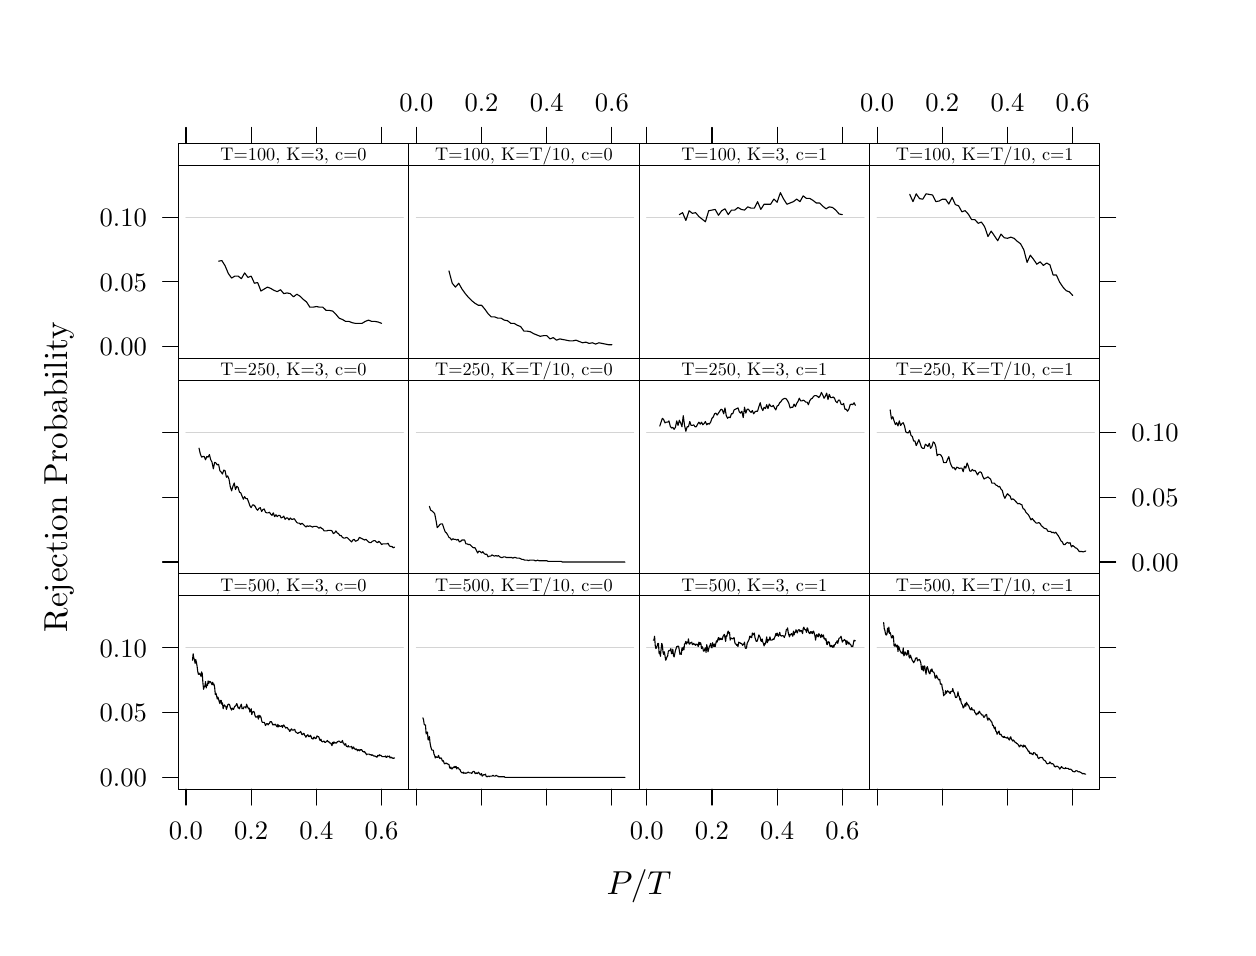
\begin{tikzpicture}[x=1pt,y=1pt]
\definecolor[named]{fillColor}{rgb}{1.00,1.00,1.00}
\path[use as bounding box,fill=fillColor,fill opacity=0.00] (0,0) rectangle (433.62,325.21);
\begin{scope}
\path[clip] (  0.00,  0.00) rectangle (433.62,325.21);

\path[] (  0.00,  0.00) rectangle (433.62,325.21);
\definecolor[named]{drawColor}{rgb}{0.00,0.00,0.00}

\node[text=drawColor,anchor=base,inner sep=0pt, outer sep=0pt, scale=  1.20] at (220.94, 12.05) {$P/T$};
\end{scope}
\begin{scope}
\path[clip] (  0.00,  0.00) rectangle (433.62,325.21);
\definecolor[named]{drawColor}{rgb}{0.00,0.00,0.00}

\node[text=drawColor,rotate= 90.00,anchor=base,inner sep=0pt, outer sep=0pt, scale=  1.20] at ( 14.29,162.76) {Rejection Probability};
\end{scope}
\begin{scope}
\path[clip] (  0.00,  0.00) rectangle (433.62,325.21);
\definecolor[named]{drawColor}{rgb}{0.00,0.00,0.00}

\path[draw=drawColor,line width= 0.4pt,line join=round,line cap=round] ( 54.44, 54.31) -- ( 48.75, 54.31);

\path[draw=drawColor,line width= 0.4pt,line join=round,line cap=round] ( 54.44, 77.70) -- ( 48.75, 77.70);

\path[draw=drawColor,line width= 0.4pt,line join=round,line cap=round] ( 54.44,101.09) -- ( 48.75,101.09);

\node[text=drawColor,anchor=base east,inner sep=0pt, outer sep=0pt, scale=  0.96] at ( 43.06, 51.00) {0.00};

\node[text=drawColor,anchor=base east,inner sep=0pt, outer sep=0pt, scale=  0.96] at ( 43.06, 74.39) {0.05};

\node[text=drawColor,anchor=base east,inner sep=0pt, outer sep=0pt, scale=  0.96] at ( 43.06, 97.78) {0.10};
\end{scope}
\begin{scope}
\path[clip] (  0.00,  0.00) rectangle (433.62,325.21);
\definecolor[named]{drawColor}{rgb}{0.00,0.00,0.00}

\path[draw=drawColor,line width= 0.4pt,line join=round,line cap=round] ( 57.20, 50.02) -- ( 57.20, 44.32);

\path[draw=drawColor,line width= 0.4pt,line join=round,line cap=round] ( 80.76, 50.02) -- ( 80.76, 44.32);

\path[draw=drawColor,line width= 0.4pt,line join=round,line cap=round] (104.31, 50.02) -- (104.31, 44.32);

\path[draw=drawColor,line width= 0.4pt,line join=round,line cap=round] (127.87, 50.02) -- (127.87, 44.32);

\node[text=drawColor,anchor=base,inner sep=0pt, outer sep=0pt, scale=  0.96] at ( 57.20, 32.02) {0.0};

\node[text=drawColor,anchor=base,inner sep=0pt, outer sep=0pt, scale=  0.96] at ( 80.76, 32.02) {0.2};

\node[text=drawColor,anchor=base,inner sep=0pt, outer sep=0pt, scale=  0.96] at (104.31, 32.02) {0.4};

\node[text=drawColor,anchor=base,inner sep=0pt, outer sep=0pt, scale=  0.96] at (127.87, 32.02) {0.6};
\end{scope}
\begin{scope}
\path[clip] ( 54.44, 50.02) rectangle (137.69,119.88);
\definecolor[named]{drawColor}{rgb}{0.83,0.83,0.83}

\path[draw=drawColor,line width= 0.4pt,line join=round,line cap=round] ( 57.20,101.09) --
	(135.72,101.09);
\definecolor[named]{drawColor}{rgb}{0.00,0.00,0.00}

\path[draw=drawColor,line width= 0.4pt,line join=round,line cap=round] ( 59.56, 96.64) --
	( 59.79, 98.98) --
	( 60.03, 97.35) --
	( 60.26, 96.88) --
	( 60.50, 95.48) --
	( 60.73, 96.88) --
	( 60.97, 95.94) --
	( 61.20, 94.54) --
	( 61.44, 92.67) --
	( 61.68, 91.50) --
	( 61.91, 91.97) --
	( 62.15, 91.50) --
	( 62.38, 91.73) --
	( 62.62, 90.80) --
	( 62.85, 92.43) --
	( 63.09, 91.73) --
	( 63.32, 88.46) --
	( 63.56, 86.12) --
	( 63.80, 87.05) --
	( 64.03, 87.29) --
	( 64.27, 88.93) --
	( 64.50, 86.59) --
	( 64.74, 87.76) --
	( 64.97, 87.52) --
	( 65.21, 89.16) --
	( 65.44, 88.22) --
	( 65.68, 88.93) --
	( 65.92, 88.93) --
	( 66.15, 88.69) --
	( 66.39, 88.22) --
	( 66.62, 87.76) --
	( 66.86, 88.69) --
	( 67.09, 87.76) --
	( 67.33, 87.99) --
	( 67.56, 86.82) --
	( 67.80, 84.25) --
	( 68.04, 84.71) --
	( 68.27, 83.78) --
	( 68.51, 82.61) --
	( 68.74, 83.31) --
	( 68.98, 82.61) --
	( 69.21, 81.67) --
	( 69.45, 80.97) --
	( 69.69, 82.14) --
	( 69.92, 82.14) --
	( 70.16, 80.74) --
	( 70.39, 81.21) --
	( 70.63, 79.10) --
	( 70.86, 80.04) --
	( 71.10, 80.50) --
	( 71.33, 80.04) --
	( 71.57, 80.04) --
	( 71.81, 78.87) --
	( 72.04, 79.57) --
	( 72.28, 80.50) --
	( 72.51, 80.74) --
	( 72.75, 80.74) --
	( 72.98, 80.50) --
	( 73.22, 79.57) --
	( 73.45, 79.10) --
	( 73.69, 78.63) --
	( 73.93, 79.33) --
	( 74.16, 79.10) --
	( 74.40, 78.87) --
	( 74.63, 79.57) --
	( 74.87, 80.04) --
	( 75.10, 80.04) --
	( 75.34, 80.50) --
	( 75.57, 80.97) --
	( 75.81, 80.27) --
	( 76.05, 79.33) --
	( 76.28, 79.57) --
	( 76.52, 79.10) --
	( 76.75, 79.80) --
	( 76.99, 80.27) --
	( 77.22, 80.74) --
	( 77.46, 79.10) --
	( 77.69, 79.33) --
	( 77.93, 79.10) --
	( 78.17, 79.80) --
	( 78.40, 79.80) --
	( 78.64, 79.80) --
	( 78.87, 79.33) --
	( 79.11, 80.74) --
	( 79.34, 80.04) --
	( 79.58, 79.57) --
	( 79.81, 79.10) --
	( 80.05, 79.33) --
	( 80.29, 77.93) --
	( 80.52, 78.17) --
	( 80.76, 79.10) --
	( 80.99, 77.00) --
	( 81.23, 77.93) --
	( 81.46, 77.93) --
	( 81.70, 78.17) --
	( 81.93, 77.70) --
	( 82.17, 76.53) --
	( 82.41, 76.06) --
	( 82.64, 76.06) --
	( 82.88, 76.29) --
	( 83.11, 76.53) --
	( 83.35, 75.36) --
	( 83.58, 76.76) --
	( 83.82, 76.06) --
	( 84.05, 76.53) --
	( 84.29, 76.06) --
	( 84.53, 74.89) --
	( 84.76, 74.19) --
	( 85.00, 74.19) --
	( 85.23, 74.19) --
	( 85.47, 74.19) --
	( 85.70, 73.72) --
	( 85.94, 73.02) --
	( 86.17, 73.49) --
	( 86.41, 73.72) --
	( 86.65, 73.72) --
	( 86.88, 73.25) --
	( 87.12, 73.72) --
	( 87.35, 73.72) --
	( 87.59, 74.42) --
	( 87.82, 74.42) --
	( 88.06, 74.42) --
	( 88.29, 73.95) --
	( 88.53, 73.25) --
	( 88.77, 73.25) --
	( 89.00, 73.49) --
	( 89.24, 73.25) --
	( 89.47, 73.49) --
	( 89.71, 73.25) --
	( 89.94, 72.79) --
	( 90.18, 72.55) --
	( 90.41, 73.49) --
	( 90.65, 72.55) --
	( 90.89, 73.02) --
	( 91.12, 72.79) --
	( 91.36, 72.79) --
	( 91.59, 72.79) --
	( 91.83, 73.02) --
	( 92.06, 72.32) --
	( 92.30, 73.02) --
	( 92.53, 73.25) --
	( 92.77, 72.79) --
	( 93.01, 72.55) --
	( 93.24, 72.08) --
	( 93.48, 72.32) --
	( 93.71, 72.32) --
	( 93.95, 72.08) --
	( 94.18, 71.62) --
	( 94.42, 71.62) --
	( 94.66, 70.91) --
	( 94.89, 71.15) --
	( 95.13, 71.62) --
	( 95.36, 71.85) --
	( 95.60, 71.38) --
	( 95.83, 71.38) --
	( 96.07, 71.38) --
	( 96.30, 71.62) --
	( 96.54, 71.62) --
	( 96.78, 70.68) --
	( 97.01, 70.68) --
	( 97.25, 70.45) --
	( 97.48, 70.21) --
	( 97.72, 70.21) --
	( 97.95, 70.45) --
	( 98.19, 70.45) --
	( 98.42, 70.68) --
	( 98.66, 70.91) --
	( 98.90, 70.21) --
	( 99.13, 69.74) --
	( 99.37, 69.74) --
	( 99.60, 70.21) --
	( 99.84, 70.21) --
	(100.07, 69.51) --
	(100.31, 69.28) --
	(100.54, 68.81) --
	(100.78, 69.28) --
	(101.02, 69.51) --
	(101.25, 69.74) --
	(101.49, 69.04) --
	(101.72, 69.28) --
	(101.96, 69.04) --
	(102.19, 69.51) --
	(102.43, 69.04) --
	(102.66, 68.34) --
	(102.90, 68.34) --
	(103.14, 68.11) --
	(103.37, 68.81) --
	(103.61, 68.81) --
	(103.84, 68.34) --
	(104.08, 68.34) --
	(104.31, 68.57) --
	(104.55, 69.28) --
	(104.78, 69.04) --
	(105.02, 69.04) --
	(105.26, 68.81) --
	(105.49, 67.87) --
	(105.73, 67.64) --
	(105.96, 68.11) --
	(106.20, 67.40) --
	(106.43, 67.17) --
	(106.67, 67.17) --
	(106.90, 67.40) --
	(107.14, 67.40) --
	(107.38, 66.94) --
	(107.61, 66.94) --
	(107.85, 67.17) --
	(108.08, 67.40) --
	(108.32, 67.64) --
	(108.55, 67.17) --
	(108.79, 67.17) --
	(109.02, 66.94) --
	(109.26, 66.70) --
	(109.50, 66.70) --
	(109.73, 66.24) --
	(109.97, 65.77) --
	(110.20, 66.94) --
	(110.44, 66.47) --
	(110.67, 67.17) --
	(110.91, 66.70) --
	(111.14, 66.70) --
	(111.38, 66.94) --
	(111.62, 66.70) --
	(111.85, 67.17) --
	(112.09, 67.17) --
	(112.32, 67.40) --
	(112.56, 67.40) --
	(112.79, 67.17) --
	(113.03, 66.94) --
	(113.26, 66.94) --
	(113.50, 67.17) --
	(113.74, 67.64) --
	(113.97, 66.70) --
	(114.21, 66.70) --
	(114.44, 66.00) --
	(114.68, 66.00) --
	(114.91, 66.47) --
	(115.15, 65.53) --
	(115.38, 65.53) --
	(115.62, 65.30) --
	(115.86, 65.77) --
	(116.09, 65.30) --
	(116.33, 65.30) --
	(116.56, 65.30) --
	(116.80, 65.30) --
	(117.03, 65.53) --
	(117.27, 64.60) --
	(117.51, 64.83) --
	(117.74, 65.30) --
	(117.98, 64.83) --
	(118.21, 64.60) --
	(118.45, 64.36) --
	(118.68, 64.60) --
	(118.92, 64.36) --
	(119.15, 63.90) --
	(119.39, 64.36) --
	(119.63, 64.13) --
	(119.86, 63.90) --
	(120.10, 64.36) --
	(120.33, 64.13) --
	(120.57, 64.36) --
	(120.80, 64.13) --
	(121.04, 63.66) --
	(121.27, 63.66) --
	(121.51, 63.43) --
	(121.75, 63.66) --
	(121.98, 63.19) --
	(122.22, 62.96) --
	(122.45, 62.49) --
	(122.69, 62.73) --
	(122.92, 62.73) --
	(123.16, 62.73) --
	(123.39, 62.73) --
	(123.63, 62.49) --
	(123.87, 62.49) --
	(124.10, 62.49) --
	(124.34, 62.26) --
	(124.57, 62.49) --
	(124.81, 62.26) --
	(125.04, 62.02) --
	(125.28, 62.02) --
	(125.51, 62.02) --
	(125.75, 61.79) --
	(125.99, 61.79) --
	(126.22, 61.56) --
	(126.46, 62.26) --
	(126.69, 62.26) --
	(126.93, 62.02) --
	(127.16, 62.49) --
	(127.40, 62.26) --
	(127.63, 62.26) --
	(127.87, 62.02) --
	(128.11, 61.79) --
	(128.34, 61.79) --
	(128.58, 61.79) --
	(128.81, 61.79) --
	(129.05, 61.79) --
	(129.28, 62.02) --
	(129.52, 61.56) --
	(129.75, 61.56) --
	(129.99, 62.02) --
	(130.23, 61.79) --
	(130.46, 61.79) --
	(130.70, 62.02) --
	(130.93, 61.32) --
	(131.17, 61.56) --
	(131.40, 61.56) --
	(131.64, 61.32) --
	(131.87, 61.32) --
	(132.11, 61.09) --
	(132.35, 61.32) --
	(132.58, 61.32);
\end{scope}
\begin{scope}
\path[clip] (  0.00,  0.00) rectangle (433.62,325.21);
\definecolor[named]{drawColor}{rgb}{0.00,0.00,0.00}

\path[draw=drawColor,line width= 0.4pt,line join=round,line cap=round] ( 54.44, 50.02) rectangle (137.69,119.88);
\end{scope}
\begin{scope}
\path[clip] ( 54.44,119.88) rectangle (137.69,127.83);

\path[] ( 54.44,119.88) rectangle (137.69,127.83);
\definecolor[named]{drawColor}{rgb}{0.00,0.00,0.00}

\node[text=drawColor,anchor=base west,inner sep=0pt, outer sep=0pt, scale=  0.66] at ( 69.67,121.58) {T=500, K=3, c=0};
\end{scope}
\begin{scope}
\path[clip] (  0.00,  0.00) rectangle (433.62,325.21);
\definecolor[named]{drawColor}{rgb}{0.00,0.00,0.00}

\path[draw=drawColor,line width= 0.4pt,line join=round,line cap=round] ( 54.44,119.88) rectangle (137.69,127.83);
\end{scope}
\begin{scope}
\path[clip] (  0.00,  0.00) rectangle (433.62,325.21);
\definecolor[named]{drawColor}{rgb}{0.00,0.00,0.00}

\path[draw=drawColor,line width= 0.4pt,line join=round,line cap=round] (140.45, 50.02) -- (140.45, 44.32);

\path[draw=drawColor,line width= 0.4pt,line join=round,line cap=round] (164.01, 50.02) -- (164.01, 44.32);

\path[draw=drawColor,line width= 0.4pt,line join=round,line cap=round] (187.56, 50.02) -- (187.56, 44.32);

\path[draw=drawColor,line width= 0.4pt,line join=round,line cap=round] (211.12, 50.02) -- (211.12, 44.32);
\end{scope}
\begin{scope}
\path[clip] (137.69, 50.02) rectangle (220.94,119.88);
\definecolor[named]{drawColor}{rgb}{0.83,0.83,0.83}

\path[draw=drawColor,line width= 0.4pt,line join=round,line cap=round] (140.45,101.09) --
	(218.97,101.09);
\definecolor[named]{drawColor}{rgb}{0.00,0.00,0.00}

\path[draw=drawColor,line width= 0.4pt,line join=round,line cap=round] (142.80, 75.83) --
	(143.04, 75.12) --
	(143.28, 73.49) --
	(143.51, 73.25) --
	(143.75, 73.25) --
	(143.98, 69.98) --
	(144.22, 70.45) --
	(144.45, 70.68) --
	(144.69, 67.87) --
	(144.92, 67.87) --
	(145.16, 69.04) --
	(145.40, 66.70) --
	(145.63, 65.53) --
	(145.87, 64.60) --
	(146.10, 64.13) --
	(146.34, 64.13) --
	(146.57, 64.13) --
	(146.81, 62.73) --
	(147.05, 62.26) --
	(147.28, 61.32) --
	(147.52, 61.79) --
	(147.75, 61.56) --
	(147.99, 61.56) --
	(148.22, 61.56) --
	(148.46, 62.26) --
	(148.69, 61.56) --
	(148.93, 61.09) --
	(149.17, 61.32) --
	(149.40, 61.32) --
	(149.64, 60.86) --
	(149.87, 60.15) --
	(150.11, 60.39) --
	(150.34, 59.92) --
	(150.58, 59.22) --
	(150.81, 59.22) --
	(151.05, 59.45) --
	(151.29, 59.45) --
	(151.52, 59.22) --
	(151.76, 59.22) --
	(151.99, 58.98) --
	(152.23, 58.98) --
	(152.46, 57.81) --
	(152.70, 57.58) --
	(152.93, 58.05) --
	(153.17, 57.35) --
	(153.41, 57.35) --
	(153.64, 57.81) --
	(153.88, 58.05) --
	(154.11, 57.81) --
	(154.35, 58.28) --
	(154.58, 57.81) --
	(154.82, 58.28) --
	(155.05, 57.35) --
	(155.29, 57.81) --
	(155.53, 57.81) --
	(155.76, 57.58) --
	(156.00, 57.11) --
	(156.23, 57.11) --
	(156.47, 56.41) --
	(156.70, 56.18) --
	(156.94, 55.94) --
	(157.17, 55.94) --
	(157.41, 56.18) --
	(157.65, 55.71) --
	(157.88, 55.94) --
	(158.12, 55.94) --
	(158.35, 55.71) --
	(158.59, 55.94) --
	(158.82, 55.94) --
	(159.06, 56.18) --
	(159.29, 56.18) --
	(159.53, 55.94) --
	(159.77, 55.94) --
	(160.00, 55.94) --
	(160.24, 55.94) --
	(160.47, 55.71) --
	(160.71, 56.18) --
	(160.94, 56.41) --
	(161.18, 56.41) --
	(161.41, 56.41) --
	(161.65, 55.71) --
	(161.89, 55.71) --
	(162.12, 55.94) --
	(162.36, 55.71) --
	(162.59, 55.71) --
	(162.83, 56.18) --
	(163.06, 55.94) --
	(163.30, 55.71) --
	(163.53, 55.24) --
	(163.77, 55.24) --
	(164.01, 55.71) --
	(164.24, 54.77) --
	(164.48, 55.01) --
	(164.71, 55.24) --
	(164.95, 55.24) --
	(165.18, 55.24) --
	(165.42, 55.48) --
	(165.65, 54.77) --
	(165.89, 54.54) --
	(166.13, 54.54) --
	(166.36, 54.77) --
	(166.60, 54.77) --
	(166.83, 54.54) --
	(167.07, 54.77) --
	(167.30, 54.77) --
	(167.54, 54.77) --
	(167.77, 54.77) --
	(168.01, 55.01) --
	(168.25, 55.01) --
	(168.48, 54.77) --
	(168.72, 54.77) --
	(168.95, 54.77) --
	(169.19, 55.01) --
	(169.42, 55.01) --
	(169.66, 54.77) --
	(169.90, 54.77) --
	(170.13, 54.54) --
	(170.37, 54.54) --
	(170.60, 54.54) --
	(170.84, 54.54) --
	(171.07, 54.54) --
	(171.31, 54.54) --
	(171.54, 54.54) --
	(171.78, 54.54) --
	(172.02, 54.54) --
	(172.25, 54.54) --
	(172.49, 54.31) --
	(172.72, 54.31) --
	(172.96, 54.31) --
	(173.19, 54.31) --
	(173.43, 54.31) --
	(173.66, 54.31) --
	(173.90, 54.31) --
	(174.14, 54.31) --
	(174.37, 54.31) --
	(174.61, 54.31) --
	(174.84, 54.31) --
	(175.08, 54.31) --
	(175.31, 54.31) --
	(175.55, 54.31) --
	(175.78, 54.31) --
	(176.02, 54.31) --
	(176.26, 54.31) --
	(176.49, 54.31) --
	(176.73, 54.31) --
	(176.96, 54.31) --
	(177.20, 54.31) --
	(177.43, 54.31) --
	(177.67, 54.31) --
	(177.90, 54.31) --
	(178.14, 54.31) --
	(178.38, 54.31) --
	(178.61, 54.31) --
	(178.85, 54.31) --
	(179.08, 54.31) --
	(179.32, 54.31) --
	(179.55, 54.31) --
	(179.79, 54.31) --
	(180.02, 54.31) --
	(180.26, 54.31) --
	(180.50, 54.31) --
	(180.73, 54.31) --
	(180.97, 54.31) --
	(181.20, 54.31) --
	(181.44, 54.31) --
	(181.67, 54.31) --
	(181.91, 54.31) --
	(182.14, 54.31) --
	(182.38, 54.31) --
	(182.62, 54.31) --
	(182.85, 54.31) --
	(183.09, 54.31) --
	(183.32, 54.31) --
	(183.56, 54.31) --
	(183.79, 54.31) --
	(184.03, 54.31) --
	(184.26, 54.31) --
	(184.50, 54.31) --
	(184.74, 54.31) --
	(184.97, 54.31) --
	(185.21, 54.31) --
	(185.44, 54.31) --
	(185.68, 54.31) --
	(185.91, 54.31) --
	(186.15, 54.31) --
	(186.38, 54.31) --
	(186.62, 54.31) --
	(186.86, 54.31) --
	(187.09, 54.31) --
	(187.33, 54.31) --
	(187.56, 54.31) --
	(187.80, 54.31) --
	(188.03, 54.31) --
	(188.27, 54.31) --
	(188.50, 54.31) --
	(188.74, 54.31) --
	(188.98, 54.31) --
	(189.21, 54.31) --
	(189.45, 54.31) --
	(189.68, 54.31) --
	(189.92, 54.31) --
	(190.15, 54.31) --
	(190.39, 54.31) --
	(190.62, 54.31) --
	(190.86, 54.31) --
	(191.10, 54.31) --
	(191.33, 54.31) --
	(191.57, 54.31) --
	(191.80, 54.31) --
	(192.04, 54.31) --
	(192.27, 54.31) --
	(192.51, 54.31) --
	(192.74, 54.31) --
	(192.98, 54.31) --
	(193.22, 54.31) --
	(193.45, 54.31) --
	(193.69, 54.31) --
	(193.92, 54.31) --
	(194.16, 54.31) --
	(194.39, 54.31) --
	(194.63, 54.31) --
	(194.87, 54.31) --
	(195.10, 54.31) --
	(195.34, 54.31) --
	(195.57, 54.31) --
	(195.81, 54.31) --
	(196.04, 54.31) --
	(196.28, 54.31) --
	(196.51, 54.31) --
	(196.75, 54.31) --
	(196.99, 54.31) --
	(197.22, 54.31) --
	(197.46, 54.31) --
	(197.69, 54.31) --
	(197.93, 54.31) --
	(198.16, 54.31) --
	(198.40, 54.31) --
	(198.63, 54.31) --
	(198.87, 54.31) --
	(199.11, 54.31) --
	(199.34, 54.31) --
	(199.58, 54.31) --
	(199.81, 54.31) --
	(200.05, 54.31) --
	(200.28, 54.31) --
	(200.52, 54.31) --
	(200.75, 54.31) --
	(200.99, 54.31) --
	(201.23, 54.31) --
	(201.46, 54.31) --
	(201.70, 54.31) --
	(201.93, 54.31) --
	(202.17, 54.31) --
	(202.40, 54.31) --
	(202.64, 54.31) --
	(202.87, 54.31) --
	(203.11, 54.31) --
	(203.35, 54.31) --
	(203.58, 54.31) --
	(203.82, 54.31) --
	(204.05, 54.31) --
	(204.29, 54.31) --
	(204.52, 54.31) --
	(204.76, 54.31) --
	(204.99, 54.31) --
	(205.23, 54.31) --
	(205.47, 54.31) --
	(205.70, 54.31) --
	(205.94, 54.31) --
	(206.17, 54.31) --
	(206.41, 54.31) --
	(206.64, 54.31) --
	(206.88, 54.31) --
	(207.11, 54.31) --
	(207.35, 54.31) --
	(207.59, 54.31) --
	(207.82, 54.31) --
	(208.06, 54.31) --
	(208.29, 54.31) --
	(208.53, 54.31) --
	(208.76, 54.31) --
	(209.00, 54.31) --
	(209.23, 54.31) --
	(209.47, 54.31) --
	(209.71, 54.31) --
	(209.94, 54.31) --
	(210.18, 54.31) --
	(210.41, 54.31) --
	(210.65, 54.31) --
	(210.88, 54.31) --
	(211.12, 54.31) --
	(211.35, 54.31) --
	(211.59, 54.31) --
	(211.83, 54.31) --
	(212.06, 54.31) --
	(212.30, 54.31) --
	(212.53, 54.31) --
	(212.77, 54.31) --
	(213.00, 54.31) --
	(213.24, 54.31) --
	(213.47, 54.31) --
	(213.71, 54.31) --
	(213.95, 54.31) --
	(214.18, 54.31) --
	(214.42, 54.31) --
	(214.65, 54.31) --
	(214.89, 54.31) --
	(215.12, 54.31) --
	(215.36, 54.31) --
	(215.59, 54.31) --
	(215.83, 54.31);
\end{scope}
\begin{scope}
\path[clip] (  0.00,  0.00) rectangle (433.62,325.21);
\definecolor[named]{drawColor}{rgb}{0.00,0.00,0.00}

\path[draw=drawColor,line width= 0.4pt,line join=round,line cap=round] (137.69, 50.02) rectangle (220.94,119.88);
\end{scope}
\begin{scope}
\path[clip] (137.69,119.88) rectangle (220.94,127.83);

\path[] (137.69,119.88) rectangle (220.94,127.83);
\definecolor[named]{drawColor}{rgb}{0.00,0.00,0.00}

\node[text=drawColor,anchor=base west,inner sep=0pt, outer sep=0pt, scale=  0.66] at (147.24,121.58) {T=500, K=T/10, c=0};
\end{scope}
\begin{scope}
\path[clip] (  0.00,  0.00) rectangle (433.62,325.21);
\definecolor[named]{drawColor}{rgb}{0.00,0.00,0.00}

\path[draw=drawColor,line width= 0.4pt,line join=round,line cap=round] (137.69,119.88) rectangle (220.94,127.83);
\end{scope}
\begin{scope}
\path[clip] (  0.00,  0.00) rectangle (433.62,325.21);
\definecolor[named]{drawColor}{rgb}{0.00,0.00,0.00}

\path[draw=drawColor,line width= 0.4pt,line join=round,line cap=round] (223.70, 50.02) -- (223.70, 44.32);

\path[draw=drawColor,line width= 0.4pt,line join=round,line cap=round] (247.26, 50.02) -- (247.26, 44.32);

\path[draw=drawColor,line width= 0.4pt,line join=round,line cap=round] (270.81, 50.02) -- (270.81, 44.32);

\path[draw=drawColor,line width= 0.4pt,line join=round,line cap=round] (294.37, 50.02) -- (294.37, 44.32);

\node[text=drawColor,anchor=base,inner sep=0pt, outer sep=0pt, scale=  0.96] at (223.70, 32.02) {0.0};

\node[text=drawColor,anchor=base,inner sep=0pt, outer sep=0pt, scale=  0.96] at (247.26, 32.02) {0.2};

\node[text=drawColor,anchor=base,inner sep=0pt, outer sep=0pt, scale=  0.96] at (270.81, 32.02) {0.4};

\node[text=drawColor,anchor=base,inner sep=0pt, outer sep=0pt, scale=  0.96] at (294.37, 32.02) {0.6};
\end{scope}
\begin{scope}
\path[clip] (220.94, 50.02) rectangle (304.19,119.88);
\definecolor[named]{drawColor}{rgb}{0.83,0.83,0.83}

\path[draw=drawColor,line width= 0.4pt,line join=round,line cap=round] (223.70,101.09) --
	(302.22,101.09);
\definecolor[named]{drawColor}{rgb}{0.00,0.00,0.00}

\path[draw=drawColor,line width= 0.4pt,line join=round,line cap=round] (226.05,103.90) --
	(226.29,103.90) --
	(226.53,105.30) --
	(226.76,102.02) --
	(227.00,100.86) --
	(227.23,101.09) --
	(227.47,101.79) --
	(227.70,102.73) --
	(227.94,102.73) --
	(228.17, 98.98) --
	(228.41, 99.69) --
	(228.65, 98.05) --
	(228.88,100.62) --
	(229.12,102.73) --
	(229.35,102.02) --
	(229.59, 99.45) --
	(229.82, 98.75) --
	(230.06, 99.69) --
	(230.29, 98.28) --
	(230.53, 96.64) --
	(230.77, 97.11) --
	(231.00, 97.81) --
	(231.24, 98.05) --
	(231.47, 99.69) --
	(231.71,100.15) --
	(231.94,100.15) --
	(232.18,100.15) --
	(232.41,100.86) --
	(232.65, 98.98) --
	(232.89, 99.22) --
	(233.12,100.62) --
	(233.36, 98.28) --
	(233.59, 97.81) --
	(233.83, 98.98) --
	(234.06,100.15) --
	(234.30,100.86) --
	(234.53,101.56) --
	(234.77,101.56) --
	(235.01,101.79) --
	(235.24,101.56) --
	(235.48,100.15) --
	(235.71, 98.75) --
	(235.95, 99.22) --
	(236.18, 98.75) --
	(236.42,101.09) --
	(236.65,100.15) --
	(236.89,101.32) --
	(237.13,100.39) --
	(237.36,102.49) --
	(237.60,102.73) --
	(237.83,103.43) --
	(238.07,102.49) --
	(238.30,103.19) --
	(238.54,102.96) --
	(238.77,104.36) --
	(239.01,102.49) --
	(239.25,102.49) --
	(239.48,102.96) --
	(239.72,102.96) --
	(239.95,103.19) --
	(240.19,102.26) --
	(240.42,102.49) --
	(240.66,102.73) --
	(240.89,102.26) --
	(241.13,102.49) --
	(241.37,102.02) --
	(241.60,102.26) --
	(241.84,102.49) --
	(242.07,102.26) --
	(242.31,101.56) --
	(242.54,103.19) --
	(242.78,102.26) --
	(243.01,102.96) --
	(243.25,102.73) --
	(243.49,100.86) --
	(243.72,101.56) --
	(243.96,101.09) --
	(244.19, 99.92) --
	(244.43, 99.92) --
	(244.66,100.62) --
	(244.90,101.09) --
	(245.13, 99.45) --
	(245.37,102.26) --
	(245.61,101.09) --
	(245.84, 99.69) --
	(246.08,100.62) --
	(246.31,101.56) --
	(246.55,102.02) --
	(246.78,102.73) --
	(247.02,101.32) --
	(247.26,101.09) --
	(247.49,102.96) --
	(247.73,102.02) --
	(247.96,101.56) --
	(248.20,102.49) --
	(248.43,101.56) --
	(248.67,102.73) --
	(248.90,103.66) --
	(249.14,103.19) --
	(249.38,104.13) --
	(249.61,104.83) --
	(249.85,103.90) --
	(250.08,104.60) --
	(250.32,104.13) --
	(250.55,104.60) --
	(250.79,104.13) --
	(251.02,104.13) --
	(251.26,105.30) --
	(251.50,105.53) --
	(251.73,106.00) --
	(251.97,104.83) --
	(252.20,103.43) --
	(252.44,105.53) --
	(252.67,105.30) --
	(252.91,106.70) --
	(253.14,107.17) --
	(253.38,106.24) --
	(253.62,106.70) --
	(253.85,103.90) --
	(254.09,104.60) --
	(254.32,104.60) --
	(254.56,104.36) --
	(254.79,104.36) --
	(255.03,104.60) --
	(255.26,104.83) --
	(255.50,103.19) --
	(255.74,102.49) --
	(255.97,102.49) --
	(256.21,102.02) --
	(256.44,102.26) --
	(256.68,101.56) --
	(256.91,103.19) --
	(257.15,102.96) --
	(257.38,102.96) --
	(257.62,102.73) --
	(257.86,102.73) --
	(258.09,102.49) --
	(258.33,102.02) --
	(258.56,102.49) --
	(258.80,102.26) --
	(259.03,103.19) --
	(259.27,101.09) --
	(259.50,100.86) --
	(259.74,101.09) --
	(259.98,102.73) --
	(260.21,103.19) --
	(260.45,103.66) --
	(260.68,104.13) --
	(260.92,105.30) --
	(261.15,105.30) --
	(261.39,104.83) --
	(261.62,104.83) --
	(261.86,106.47) --
	(262.10,105.77) --
	(262.33,106.00) --
	(262.57,106.47) --
	(262.80,104.83) --
	(263.04,104.13) --
	(263.27,103.43) --
	(263.51,103.43) --
	(263.74,103.90) --
	(263.98,104.83) --
	(264.22,105.77) --
	(264.45,105.30) --
	(264.69,104.83) --
	(264.92,103.66) --
	(265.16,103.43) --
	(265.39,104.36) --
	(265.63,103.19) --
	(265.86,102.73) --
	(266.10,101.79) --
	(266.34,102.73) --
	(266.57,102.49) --
	(266.81,103.66) --
	(267.04,105.07) --
	(267.28,102.96) --
	(267.51,104.13) --
	(267.75,103.66) --
	(267.98,104.13) --
	(268.22,105.07) --
	(268.46,103.90) --
	(268.69,103.90) --
	(268.93,103.90) --
	(269.16,104.13) --
	(269.40,104.36) --
	(269.63,104.13) --
	(269.87,104.83) --
	(270.11,105.30) --
	(270.34,106.24) --
	(270.58,105.53) --
	(270.81,106.47) --
	(271.05,105.77) --
	(271.28,105.30) --
	(271.52,106.00) --
	(271.75,106.70) --
	(271.99,105.53) --
	(272.23,105.53) --
	(272.46,105.30) --
	(272.70,105.53) --
	(272.93,105.53) --
	(273.17,105.30) --
	(273.40,104.83) --
	(273.64,105.53) --
	(273.87,106.00) --
	(274.11,107.64) --
	(274.35,107.64) --
	(274.58,108.34) --
	(274.82,106.70) --
	(275.05,105.77) --
	(275.29,105.07) --
	(275.52,106.00) --
	(275.76,105.77) --
	(275.99,106.24) --
	(276.23,106.00) --
	(276.47,105.30) --
	(276.70,107.17) --
	(276.94,105.77) --
	(277.17,106.70) --
	(277.41,106.70) --
	(277.64,107.64) --
	(277.88,106.94) --
	(278.11,106.47) --
	(278.35,107.40) --
	(278.59,107.64) --
	(278.82,107.64) --
	(279.06,106.94) --
	(279.29,107.40) --
	(279.53,107.40) --
	(279.76,106.94) --
	(280.00,106.24) --
	(280.23,108.11) --
	(280.47,108.57) --
	(280.71,107.87) --
	(280.94,107.64) --
	(281.18,107.64) --
	(281.41,106.70) --
	(281.65,108.34) --
	(281.88,108.11) --
	(282.12,106.94) --
	(282.35,106.47) --
	(282.59,106.24) --
	(282.83,106.94) --
	(283.06,106.47) --
	(283.30,106.94) --
	(283.53,106.24) --
	(283.77,106.94) --
	(284.00,107.17) --
	(284.24,106.24) --
	(284.47,105.53) --
	(284.71,103.90) --
	(284.95,105.53) --
	(285.18,106.00) --
	(285.42,105.30) --
	(285.65,105.07) --
	(285.89,106.24) --
	(286.12,105.77) --
	(286.36,105.30) --
	(286.59,104.83) --
	(286.83,106.00) --
	(287.07,105.07) --
	(287.30,105.30) --
	(287.54,105.77) --
	(287.77,104.36) --
	(288.01,104.60) --
	(288.24,103.90) --
	(288.48,104.36) --
	(288.71,102.49) --
	(288.95,102.26) --
	(289.19,103.43) --
	(289.42,102.96) --
	(289.66,103.19) --
	(289.89,101.79) --
	(290.13,101.56) --
	(290.36,102.02) --
	(290.60,101.56) --
	(290.83,101.32) --
	(291.07,102.02) --
	(291.31,101.32) --
	(291.54,102.26) --
	(291.78,102.26) --
	(292.01,102.96) --
	(292.25,102.96) --
	(292.48,103.66) --
	(292.72,102.73) --
	(292.96,103.66) --
	(293.19,104.60) --
	(293.43,104.60) --
	(293.66,104.83) --
	(293.90,105.30) --
	(294.13,104.36) --
	(294.37,103.19) --
	(294.60,103.66) --
	(294.84,103.66) --
	(295.08,104.13) --
	(295.31,103.90) --
	(295.55,103.66) --
	(295.78,102.26) --
	(296.02,103.66) --
	(296.25,103.19) --
	(296.49,102.49) --
	(296.72,103.19) --
	(296.96,102.49) --
	(297.20,102.49) --
	(297.43,102.26) --
	(297.67,101.56) --
	(297.90,101.79) --
	(298.14,101.56) --
	(298.37,102.73) --
	(298.61,103.90) --
	(298.84,103.66) --
	(299.08,103.66);
\end{scope}
\begin{scope}
\path[clip] (  0.00,  0.00) rectangle (433.62,325.21);
\definecolor[named]{drawColor}{rgb}{0.00,0.00,0.00}

\path[draw=drawColor,line width= 0.4pt,line join=round,line cap=round] (220.94, 50.02) rectangle (304.19,119.88);
\end{scope}
\begin{scope}
\path[clip] (220.94,119.88) rectangle (304.19,127.83);

\path[] (220.94,119.88) rectangle (304.19,127.83);
\definecolor[named]{drawColor}{rgb}{0.00,0.00,0.00}

\node[text=drawColor,anchor=base west,inner sep=0pt, outer sep=0pt, scale=  0.66] at (236.17,121.58) {T=500, K=3, c=1};
\end{scope}
\begin{scope}
\path[clip] (  0.00,  0.00) rectangle (433.62,325.21);
\definecolor[named]{drawColor}{rgb}{0.00,0.00,0.00}

\path[draw=drawColor,line width= 0.4pt,line join=round,line cap=round] (220.94,119.88) rectangle (304.19,127.83);
\end{scope}
\begin{scope}
\path[clip] (  0.00,  0.00) rectangle (433.62,325.21);
\definecolor[named]{drawColor}{rgb}{0.00,0.00,0.00}

\path[draw=drawColor,line width= 0.4pt,line join=round,line cap=round] (306.95, 50.02) -- (306.95, 44.32);

\path[draw=drawColor,line width= 0.4pt,line join=round,line cap=round] (330.50, 50.02) -- (330.50, 44.32);

\path[draw=drawColor,line width= 0.4pt,line join=round,line cap=round] (354.06, 50.02) -- (354.06, 44.32);

\path[draw=drawColor,line width= 0.4pt,line join=round,line cap=round] (377.62, 50.02) -- (377.62, 44.32);

\path[draw=drawColor,line width= 0.4pt,line join=round,line cap=round] (387.44, 54.31) -- (393.13, 54.31);

\path[draw=drawColor,line width= 0.4pt,line join=round,line cap=round] (387.44, 77.70) -- (393.13, 77.70);

\path[draw=drawColor,line width= 0.4pt,line join=round,line cap=round] (387.44,101.09) -- (393.13,101.09);
\end{scope}
\begin{scope}
\path[clip] (304.19, 50.02) rectangle (387.44,119.88);
\definecolor[named]{drawColor}{rgb}{0.83,0.83,0.83}

\path[draw=drawColor,line width= 0.4pt,line join=round,line cap=round] (306.95,101.09) --
	(385.47,101.09);
\definecolor[named]{drawColor}{rgb}{0.00,0.00,0.00}

\path[draw=drawColor,line width= 0.4pt,line join=round,line cap=round] (309.30,110.28) --
	(309.54,107.95) --
	(309.77,107.30) --
	(310.01,106.00) --
	(310.25,105.74) --
	(310.48,106.00) --
	(310.72,108.21) --
	(310.95,106.78) --
	(311.19,108.60) --
	(311.42,106.26) --
	(311.66,106.65) --
	(311.89,105.87) --
	(312.13,104.70) --
	(312.37,104.70) --
	(312.60,105.61) --
	(312.84,105.09) --
	(313.07,101.84) --
	(313.31,101.71) --
	(313.54,102.49) --
	(313.78,101.71) --
	(314.01,101.45) --
	(314.25,102.10) --
	(314.49, 99.76) --
	(314.72,101.71) --
	(314.96,100.93) --
	(315.19,100.15) --
	(315.43, 99.76) --
	(315.66, 99.24) --
	(315.90, 99.50) --
	(316.13, 98.98) --
	(316.37,101.06) --
	(316.61, 98.21) --
	(316.84, 98.60) --
	(317.08, 99.63) --
	(317.31, 99.24) --
	(317.55, 98.47) --
	(317.78, 98.60) --
	(318.02,100.15) --
	(318.25,100.02) --
	(318.49, 97.82) --
	(318.73, 97.43) --
	(318.96, 98.47) --
	(319.20, 97.82) --
	(319.43, 97.17) --
	(319.67, 96.52) --
	(319.90, 96.26) --
	(320.14, 95.74) --
	(320.37, 96.13) --
	(320.61, 96.52) --
	(320.85, 97.43) --
	(321.08, 97.30) --
	(321.32, 97.56) --
	(321.55, 96.39) --
	(321.79, 96.78) --
	(322.02, 96.78) --
	(322.26, 96.91) --
	(322.50, 96.39) --
	(322.73, 95.74) --
	(322.97, 93.53) --
	(323.20, 93.14) --
	(323.44, 94.57) --
	(323.67, 92.75) --
	(323.91, 94.44) --
	(324.14, 94.57) --
	(324.38, 92.88) --
	(324.62, 91.58) --
	(324.85, 93.79) --
	(325.09, 94.31) --
	(325.32, 93.53) --
	(325.56, 92.49) --
	(325.79, 91.97) --
	(326.03, 91.71) --
	(326.26, 93.14) --
	(326.50, 92.62) --
	(326.74, 93.53) --
	(326.97, 92.62) --
	(327.21, 92.36) --
	(327.44, 92.36) --
	(327.68, 91.58) --
	(327.91, 90.15) --
	(328.15, 90.15) --
	(328.38, 91.19) --
	(328.62, 90.67) --
	(328.86, 90.15) --
	(329.09, 89.63) --
	(329.33, 89.50) --
	(329.56, 89.76) --
	(329.80, 88.07) --
	(330.03, 87.95) --
	(330.27, 88.07) --
	(330.50, 86.52) --
	(330.74, 85.74) --
	(330.98, 83.79) --
	(331.21, 84.18) --
	(331.45, 84.18) --
	(331.68, 85.61) --
	(331.92, 84.70) --
	(332.15, 85.22) --
	(332.39, 85.61) --
	(332.62, 85.22) --
	(332.86, 85.35) --
	(333.10, 84.83) --
	(333.33, 84.57) --
	(333.57, 85.35) --
	(333.80, 85.35) --
	(334.04, 85.35) --
	(334.27, 86.39) --
	(334.51, 85.35) --
	(334.74, 84.96) --
	(334.98, 84.44) --
	(335.22, 83.27) --
	(335.45, 83.14) --
	(335.69, 83.27) --
	(335.92, 83.79) --
	(336.16, 85.22) --
	(336.39, 83.79) --
	(336.63, 83.53) --
	(336.86, 82.23) --
	(337.10, 82.75) --
	(337.34, 81.19) --
	(337.57, 80.80) --
	(337.81, 80.41) --
	(338.04, 79.37) --
	(338.28, 79.63) --
	(338.51, 80.28) --
	(338.75, 80.93) --
	(338.98, 80.02) --
	(339.22, 81.45) --
	(339.46, 80.93) --
	(339.69, 80.54) --
	(339.93, 80.41) --
	(340.16, 79.89) --
	(340.40, 79.24) --
	(340.63, 78.85) --
	(340.87, 78.72) --
	(341.10, 79.50) --
	(341.34, 78.85) --
	(341.58, 78.59) --
	(341.81, 78.72) --
	(342.05, 78.59) --
	(342.28, 77.68) --
	(342.52, 77.55) --
	(342.75, 76.91) --
	(342.99, 77.03) --
	(343.22, 77.55) --
	(343.46, 77.29) --
	(343.70, 77.94) --
	(343.93, 78.20) --
	(344.17, 77.55) --
	(344.40, 77.42) --
	(344.64, 77.03) --
	(344.87, 76.78) --
	(345.11, 76.91) --
	(345.35, 76.26) --
	(345.58, 76.00) --
	(345.82, 76.26) --
	(346.05, 76.78) --
	(346.29, 76.91) --
	(346.52, 77.03) --
	(346.76, 75.48) --
	(346.99, 74.96) --
	(347.23, 75.74) --
	(347.47, 75.48) --
	(347.70, 75.09) --
	(347.94, 74.96) --
	(348.17, 74.44) --
	(348.41, 74.31) --
	(348.64, 73.14) --
	(348.88, 73.14) --
	(349.11, 72.49) --
	(349.35, 71.84) --
	(349.59, 72.49) --
	(349.82, 71.06) --
	(350.06, 70.80) --
	(350.29, 69.89) --
	(350.53, 70.28) --
	(350.76, 70.80) --
	(351.00, 71.06) --
	(351.23, 69.89) --
	(351.47, 69.76) --
	(351.71, 69.89) --
	(351.94, 69.37) --
	(352.18, 68.98) --
	(352.41, 68.98) --
	(352.65, 68.72) --
	(352.88, 69.11) --
	(353.12, 68.72) --
	(353.35, 68.72) --
	(353.59, 68.59) --
	(353.83, 68.46) --
	(354.06, 68.85) --
	(354.30, 68.46) --
	(354.53, 68.07) --
	(354.77, 67.81) --
	(355.00, 68.72) --
	(355.24, 68.98) --
	(355.47, 68.07) --
	(355.71, 67.81) --
	(355.95, 67.42) --
	(356.18, 67.81) --
	(356.42, 67.55) --
	(356.65, 67.16) --
	(356.89, 66.90) --
	(357.12, 66.90) --
	(357.36, 66.51) --
	(357.59, 66.51) --
	(357.83, 66.25) --
	(358.07, 65.87) --
	(358.30, 65.35) --
	(358.54, 65.48) --
	(358.77, 65.99) --
	(359.01, 65.74) --
	(359.24, 65.87) --
	(359.48, 65.48) --
	(359.71, 65.22) --
	(359.95, 65.99) --
	(360.19, 65.48) --
	(360.42, 65.74) --
	(360.66, 65.22) --
	(360.89, 64.83) --
	(361.13, 64.57) --
	(361.36, 64.18) --
	(361.60, 63.66) --
	(361.83, 63.79) --
	(362.07, 63.01) --
	(362.31, 62.88) --
	(362.54, 63.14) --
	(362.78, 62.75) --
	(363.01, 62.75) --
	(363.25, 62.49) --
	(363.48, 63.27) --
	(363.72, 63.14) --
	(363.95, 63.14) --
	(364.19, 62.62) --
	(364.43, 62.36) --
	(364.66, 62.62) --
	(364.90, 61.84) --
	(365.13, 61.32) --
	(365.37, 61.06) --
	(365.60, 61.32) --
	(365.84, 61.58) --
	(366.07, 61.45) --
	(366.31, 61.45) --
	(366.55, 61.58) --
	(366.78, 61.32) --
	(367.02, 60.67) --
	(367.25, 60.54) --
	(367.49, 60.41) --
	(367.72, 60.28) --
	(367.96, 59.89) --
	(368.19, 59.37) --
	(368.43, 59.24) --
	(368.67, 59.24) --
	(368.90, 59.37) --
	(369.14, 59.37) --
	(369.37, 59.89) --
	(369.61, 59.63) --
	(369.84, 59.24) --
	(370.08, 59.24) --
	(370.32, 59.24) --
	(370.55, 59.11) --
	(370.79, 58.85) --
	(371.02, 58.20) --
	(371.26, 58.33) --
	(371.49, 58.07) --
	(371.73, 58.33) --
	(371.96, 58.33) --
	(372.20, 58.20) --
	(372.44, 58.07) --
	(372.67, 57.81) --
	(372.91, 57.29) --
	(373.14, 57.55) --
	(373.38, 57.94) --
	(373.61, 58.20) --
	(373.85, 57.81) --
	(374.08, 57.68) --
	(374.32, 57.55) --
	(374.56, 57.55) --
	(374.79, 57.42) --
	(375.03, 57.81) --
	(375.26, 57.55) --
	(375.50, 57.55) --
	(375.73, 57.55) --
	(375.97, 57.55) --
	(376.20, 57.29) --
	(376.44, 57.16) --
	(376.68, 57.29) --
	(376.91, 57.29) --
	(377.15, 57.03) --
	(377.38, 56.90) --
	(377.62, 56.51) --
	(377.85, 56.38) --
	(378.09, 56.38) --
	(378.32, 56.25) --
	(378.56, 56.51) --
	(378.80, 56.77) --
	(379.03, 56.64) --
	(379.27, 56.64) --
	(379.50, 56.38) --
	(379.74, 56.25) --
	(379.97, 56.38) --
	(380.21, 56.25) --
	(380.44, 56.12) --
	(380.68, 55.99) --
	(380.92, 55.86) --
	(381.15, 55.60) --
	(381.39, 55.60) --
	(381.62, 55.73) --
	(381.86, 55.60) --
	(382.09, 55.47) --
	(382.33, 55.47);
\end{scope}
\begin{scope}
\path[clip] (  0.00,  0.00) rectangle (433.62,325.21);
\definecolor[named]{drawColor}{rgb}{0.00,0.00,0.00}

\path[draw=drawColor,line width= 0.4pt,line join=round,line cap=round] (304.19, 50.02) rectangle (387.44,119.88);
\end{scope}
\begin{scope}
\path[clip] (304.19,119.88) rectangle (387.44,127.83);

\path[] (304.19,119.88) rectangle (387.44,127.83);
\definecolor[named]{drawColor}{rgb}{0.00,0.00,0.00}

\node[text=drawColor,anchor=base west,inner sep=0pt, outer sep=0pt, scale=  0.66] at (313.74,121.58) {T=500, K=T/10, c=1};
\end{scope}
\begin{scope}
\path[clip] (  0.00,  0.00) rectangle (433.62,325.21);
\definecolor[named]{drawColor}{rgb}{0.00,0.00,0.00}

\path[draw=drawColor,line width= 0.4pt,line join=round,line cap=round] (304.19,119.88) rectangle (387.44,127.83);
\end{scope}
\begin{scope}
\path[clip] (  0.00,  0.00) rectangle (433.62,325.21);
\definecolor[named]{drawColor}{rgb}{0.00,0.00,0.00}

\path[draw=drawColor,line width= 0.4pt,line join=round,line cap=round] ( 54.44,132.12) -- ( 48.75,132.12);

\path[draw=drawColor,line width= 0.4pt,line join=round,line cap=round] ( 54.44,155.51) -- ( 48.75,155.51);

\path[draw=drawColor,line width= 0.4pt,line join=round,line cap=round] ( 54.44,178.91) -- ( 48.75,178.91);
\end{scope}
\begin{scope}
\path[clip] ( 54.44,127.83) rectangle (137.69,197.70);
\definecolor[named]{drawColor}{rgb}{0.83,0.83,0.83}

\path[draw=drawColor,line width= 0.4pt,line join=round,line cap=round] ( 57.20,178.91) --
	(135.72,178.91);
\definecolor[named]{drawColor}{rgb}{0.00,0.00,0.00}

\path[draw=drawColor,line width= 0.4pt,line join=round,line cap=round] ( 61.91,173.29) --
	( 62.38,171.19) --
	( 62.85,170.02) --
	( 63.32,170.25) --
	( 63.80,170.25) --
	( 64.27,169.08) --
	( 64.74,170.25) --
	( 65.21,170.02) --
	( 65.68,170.95) --
	( 66.15,169.08) --
	( 66.62,168.15) --
	( 67.09,165.81) --
	( 67.56,168.15) --
	( 68.04,167.91) --
	( 68.51,167.21) --
	( 68.98,167.44) --
	( 69.45,165.10) --
	( 69.92,164.64) --
	( 70.39,163.93) --
	( 70.86,165.34) --
	( 71.33,165.10) --
	( 71.81,162.76) --
	( 72.28,163.23) --
	( 72.75,162.06) --
	( 73.22,159.26) --
	( 73.69,157.85) --
	( 74.16,159.49) --
	( 74.63,160.66) --
	( 75.10,158.32) --
	( 75.57,159.49) --
	( 76.05,159.02) --
	( 76.52,157.38) --
	( 76.99,157.15) --
	( 77.46,155.98) --
	( 77.93,154.81) --
	( 78.40,155.75) --
	( 78.87,155.05) --
	( 79.34,155.05) --
	( 79.81,153.88) --
	( 80.29,152.47) --
	( 80.76,151.77) --
	( 81.23,152.71) --
	( 81.70,152.71) --
	( 82.17,152.24) --
	( 82.64,151.30) --
	( 83.11,150.84) --
	( 83.58,151.54) --
	( 84.05,151.77) --
	( 84.53,150.37) --
	( 85.00,151.07) --
	( 85.47,151.30) --
	( 85.94,150.13) --
	( 86.41,149.90) --
	( 86.88,149.90) --
	( 87.35,150.13) --
	( 87.82,149.43) --
	( 88.29,148.96) --
	( 88.77,149.90) --
	( 89.24,148.50) --
	( 89.71,149.20) --
	( 90.18,148.50) --
	( 90.65,148.96) --
	( 91.12,148.96) --
	( 91.59,148.03) --
	( 92.06,148.26) --
	( 92.53,148.73) --
	( 93.01,147.56) --
	( 93.48,148.03) --
	( 93.95,148.03) --
	( 94.42,147.33) --
	( 94.89,148.03) --
	( 95.36,147.56) --
	( 95.83,147.56) --
	( 96.30,147.79) --
	( 96.78,147.09) --
	( 97.25,146.39) --
	( 97.72,146.16) --
	( 98.19,146.16) --
	( 98.66,145.69) --
	( 99.13,146.16) --
	( 99.60,145.69) --
	(100.07,145.22) --
	(100.54,144.75) --
	(101.02,145.22) --
	(101.49,144.99) --
	(101.96,145.22) --
	(102.43,144.99) --
	(102.90,144.75) --
	(103.37,144.99) --
	(103.84,144.99) --
	(104.31,144.99) --
	(104.78,144.75) --
	(105.26,144.29) --
	(105.73,144.75) --
	(106.20,144.29) --
	(106.67,144.05) --
	(107.14,143.35) --
	(107.61,143.35) --
	(108.08,143.35) --
	(108.55,143.58) --
	(109.02,143.58) --
	(109.50,143.58) --
	(109.97,143.35) --
	(110.44,142.41) --
	(110.91,142.65) --
	(111.38,143.35) --
	(111.85,142.65) --
	(112.32,142.41) --
	(112.79,141.71) --
	(113.26,141.71) --
	(113.74,141.01) --
	(114.21,140.78) --
	(114.68,140.78) --
	(115.15,141.01) --
	(115.62,140.78) --
	(116.09,140.31) --
	(116.56,139.84) --
	(117.03,139.37) --
	(117.51,140.07) --
	(117.98,140.31) --
	(118.45,139.61) --
	(118.92,139.84) --
	(119.39,140.07) --
	(119.86,141.01) --
	(120.33,140.78) --
	(120.80,140.54) --
	(121.27,140.31) --
	(121.75,140.07) --
	(122.22,140.31) --
	(122.69,139.84) --
	(123.16,139.37) --
	(123.63,139.14) --
	(124.10,139.14) --
	(124.57,139.61) --
	(125.04,139.84) --
	(125.51,139.84) --
	(125.99,139.37) --
	(126.46,139.14) --
	(126.93,139.61) --
	(127.40,139.14) --
	(127.87,138.44) --
	(128.34,138.67) --
	(128.81,138.67) --
	(129.28,138.67) --
	(129.75,138.67) --
	(130.23,138.91) --
	(130.70,137.97) --
	(131.17,137.74) --
	(131.64,137.74) --
	(132.11,137.27) --
	(132.58,137.50);
\end{scope}
\begin{scope}
\path[clip] (  0.00,  0.00) rectangle (433.62,325.21);
\definecolor[named]{drawColor}{rgb}{0.00,0.00,0.00}

\path[draw=drawColor,line width= 0.4pt,line join=round,line cap=round] ( 54.44,127.83) rectangle (137.69,197.70);
\end{scope}
\begin{scope}
\path[clip] ( 54.44,197.70) rectangle (137.69,205.65);

\path[] ( 54.44,197.70) rectangle (137.69,205.65);
\definecolor[named]{drawColor}{rgb}{0.00,0.00,0.00}

\node[text=drawColor,anchor=base west,inner sep=0pt, outer sep=0pt, scale=  0.66] at ( 69.67,199.40) {T=250, K=3, c=0};
\end{scope}
\begin{scope}
\path[clip] (  0.00,  0.00) rectangle (433.62,325.21);
\definecolor[named]{drawColor}{rgb}{0.00,0.00,0.00}

\path[draw=drawColor,line width= 0.4pt,line join=round,line cap=round] ( 54.44,197.70) rectangle (137.69,205.65);
\end{scope}
\begin{scope}
\path[clip] (137.69,127.83) rectangle (220.94,197.70);
\definecolor[named]{drawColor}{rgb}{0.83,0.83,0.83}

\path[draw=drawColor,line width= 0.4pt,line join=round,line cap=round] (140.45,178.91) --
	(218.97,178.91);
\definecolor[named]{drawColor}{rgb}{0.00,0.00,0.00}

\path[draw=drawColor,line width= 0.4pt,line join=round,line cap=round] (145.16,152.24) --
	(145.63,150.84) --
	(146.10,150.60) --
	(146.57,150.13) --
	(147.05,149.67) --
	(147.52,147.33) --
	(147.99,144.52) --
	(148.46,144.99) --
	(148.93,145.69) --
	(149.40,145.92) --
	(149.87,145.92) --
	(150.34,144.52) --
	(150.81,143.12) --
	(151.29,142.65) --
	(151.76,141.95) --
	(152.23,141.01) --
	(152.70,140.78) --
	(153.17,140.07) --
	(153.64,140.54) --
	(154.11,140.31) --
	(154.58,140.31) --
	(155.05,140.07) --
	(155.53,140.31) --
	(156.00,139.37) --
	(156.47,139.61) --
	(156.94,140.07) --
	(157.41,140.07) --
	(157.88,140.07) --
	(158.35,138.67) --
	(158.82,138.67) --
	(159.29,138.44) --
	(159.77,138.44) --
	(160.24,137.97) --
	(160.71,137.50) --
	(161.18,137.27) --
	(161.65,137.27) --
	(162.12,136.33) --
	(162.59,135.40) --
	(163.06,136.10) --
	(163.53,135.86) --
	(164.01,135.40) --
	(164.48,135.86) --
	(164.95,135.16) --
	(165.42,134.93) --
	(165.89,134.93) --
	(166.36,133.99) --
	(166.83,134.23) --
	(167.30,134.23) --
	(167.77,134.69) --
	(168.25,134.46) --
	(168.72,134.23) --
	(169.19,134.46) --
	(169.66,134.23) --
	(170.13,134.46) --
	(170.60,133.99) --
	(171.07,133.76) --
	(171.54,133.76) --
	(172.02,133.99) --
	(172.49,133.99) --
	(172.96,133.76) --
	(173.43,133.76) --
	(173.90,133.76) --
	(174.37,133.76) --
	(174.84,133.76) --
	(175.31,133.53) --
	(175.78,133.76) --
	(176.26,133.76) --
	(176.73,133.53) --
	(177.20,133.53) --
	(177.67,133.53) --
	(178.14,133.29) --
	(178.61,133.06) --
	(179.08,133.06) --
	(179.55,132.82) --
	(180.02,132.82) --
	(180.50,132.82) --
	(180.97,132.59) --
	(181.44,132.82) --
	(181.91,132.82) --
	(182.38,132.82) --
	(182.85,132.82) --
	(183.32,132.59) --
	(183.79,132.59) --
	(184.26,132.82) --
	(184.74,132.59) --
	(185.21,132.59) --
	(185.68,132.59) --
	(186.15,132.59) --
	(186.62,132.59) --
	(187.09,132.59) --
	(187.56,132.59) --
	(188.03,132.36) --
	(188.50,132.36) --
	(188.98,132.36) --
	(189.45,132.36) --
	(189.92,132.36) --
	(190.39,132.36) --
	(190.86,132.36) --
	(191.33,132.36) --
	(191.80,132.36) --
	(192.27,132.36) --
	(192.74,132.36) --
	(193.22,132.12) --
	(193.69,132.12) --
	(194.16,132.12) --
	(194.63,132.12) --
	(195.10,132.12) --
	(195.57,132.12) --
	(196.04,132.12) --
	(196.51,132.12) --
	(196.99,132.12) --
	(197.46,132.12) --
	(197.93,132.12) --
	(198.40,132.12) --
	(198.87,132.12) --
	(199.34,132.12) --
	(199.81,132.12) --
	(200.28,132.12) --
	(200.75,132.12) --
	(201.23,132.12) --
	(201.70,132.12) --
	(202.17,132.12) --
	(202.64,132.12) --
	(203.11,132.12) --
	(203.58,132.12) --
	(204.05,132.12) --
	(204.52,132.12) --
	(204.99,132.12) --
	(205.47,132.12) --
	(205.94,132.12) --
	(206.41,132.12) --
	(206.88,132.12) --
	(207.35,132.12) --
	(207.82,132.12) --
	(208.29,132.12) --
	(208.76,132.12) --
	(209.23,132.12) --
	(209.71,132.12) --
	(210.18,132.12) --
	(210.65,132.12) --
	(211.12,132.12) --
	(211.59,132.12) --
	(212.06,132.12) --
	(212.53,132.12) --
	(213.00,132.12) --
	(213.47,132.12) --
	(213.95,132.12) --
	(214.42,132.12) --
	(214.89,132.12) --
	(215.36,132.12) --
	(215.83,132.12);
\end{scope}
\begin{scope}
\path[clip] (  0.00,  0.00) rectangle (433.62,325.21);
\definecolor[named]{drawColor}{rgb}{0.00,0.00,0.00}

\path[draw=drawColor,line width= 0.4pt,line join=round,line cap=round] (137.69,127.83) rectangle (220.94,197.70);
\end{scope}
\begin{scope}
\path[clip] (137.69,197.70) rectangle (220.94,205.65);

\path[] (137.69,197.70) rectangle (220.94,205.65);
\definecolor[named]{drawColor}{rgb}{0.00,0.00,0.00}

\node[text=drawColor,anchor=base west,inner sep=0pt, outer sep=0pt, scale=  0.66] at (147.24,199.40) {T=250, K=T/10, c=0};
\end{scope}
\begin{scope}
\path[clip] (  0.00,  0.00) rectangle (433.62,325.21);
\definecolor[named]{drawColor}{rgb}{0.00,0.00,0.00}

\path[draw=drawColor,line width= 0.4pt,line join=round,line cap=round] (137.69,197.70) rectangle (220.94,205.65);
\end{scope}
\begin{scope}
\path[clip] (220.94,127.83) rectangle (304.19,197.70);
\definecolor[named]{drawColor}{rgb}{0.83,0.83,0.83}

\path[draw=drawColor,line width= 0.4pt,line join=round,line cap=round] (223.70,178.91) --
	(302.22,178.91);
\definecolor[named]{drawColor}{rgb}{0.00,0.00,0.00}

\path[draw=drawColor,line width= 0.4pt,line join=round,line cap=round] (228.41,181.24) --
	(228.88,182.65) --
	(229.35,184.05) --
	(229.82,183.58) --
	(230.29,182.41) --
	(230.77,182.65) --
	(231.24,182.65) --
	(231.71,183.12) --
	(232.18,181.24) --
	(232.65,180.54) --
	(233.12,180.78) --
	(233.59,180.07) --
	(234.06,180.78) --
	(234.53,183.12) --
	(235.01,181.48) --
	(235.48,183.35) --
	(235.95,182.41) --
	(236.42,181.01) --
	(236.89,184.99) --
	(237.36,181.48) --
	(237.83,179.37) --
	(238.30,181.01) --
	(238.77,181.01) --
	(239.25,182.88) --
	(239.72,181.48) --
	(240.19,181.48) --
	(240.66,181.71) --
	(241.13,181.01) --
	(241.60,181.01) --
	(242.07,181.95) --
	(242.54,182.65) --
	(243.01,181.95) --
	(243.49,182.65) --
	(243.96,181.71) --
	(244.43,182.18) --
	(244.90,182.88) --
	(245.37,181.71) --
	(245.84,182.18) --
	(246.31,181.95) --
	(246.78,182.65) --
	(247.26,184.05) --
	(247.73,184.52) --
	(248.20,185.69) --
	(248.67,185.92) --
	(249.14,185.22) --
	(249.61,185.92) --
	(250.08,186.62) --
	(250.55,187.33) --
	(251.02,187.09) --
	(251.50,185.69) --
	(251.97,187.79) --
	(252.44,184.99) --
	(252.91,184.05) --
	(253.38,184.52) --
	(253.85,184.29) --
	(254.32,185.69) --
	(254.79,185.69) --
	(255.26,187.09) --
	(255.74,187.33) --
	(256.21,187.56) --
	(256.68,187.79) --
	(257.15,186.39) --
	(257.62,185.92) --
	(258.09,186.62) --
	(258.56,184.29) --
	(259.03,188.03) --
	(259.50,185.92) --
	(259.98,187.33) --
	(260.45,187.33) --
	(260.92,186.62) --
	(261.39,186.16) --
	(261.86,186.86) --
	(262.33,185.69) --
	(262.80,186.39) --
	(263.27,186.62) --
	(263.74,186.62) --
	(264.22,188.26) --
	(264.69,189.67) --
	(265.16,187.79) --
	(265.63,186.86) --
	(266.10,188.03) --
	(266.57,187.56) --
	(267.04,188.96) --
	(267.51,187.56) --
	(267.98,189.20) --
	(268.46,188.50) --
	(268.93,188.26) --
	(269.40,188.73) --
	(269.87,187.79) --
	(270.34,187.09) --
	(270.81,188.50) --
	(271.28,188.73) --
	(271.75,189.67) --
	(272.23,190.13) --
	(272.70,190.84) --
	(273.17,191.07) --
	(273.64,191.30) --
	(274.11,191.07) --
	(274.58,190.37) --
	(275.05,189.43) --
	(275.52,187.79) --
	(275.99,188.03) --
	(276.47,188.03) --
	(276.94,189.20) --
	(277.41,188.26) --
	(277.88,189.43) --
	(278.35,190.13) --
	(278.82,191.30) --
	(279.29,190.37) --
	(279.76,190.37) --
	(280.23,190.60) --
	(280.71,190.37) --
	(281.18,189.90) --
	(281.65,189.90) --
	(282.12,188.96) --
	(282.59,190.37) --
	(283.06,191.07) --
	(283.53,191.30) --
	(284.00,192.00) --
	(284.47,192.24) --
	(284.95,192.24) --
	(285.42,192.00) --
	(285.89,191.54) --
	(286.36,192.24) --
	(286.83,193.41) --
	(287.30,192.47) --
	(287.77,191.30) --
	(288.24,192.00) --
	(288.71,193.17) --
	(289.19,190.84) --
	(289.66,192.71) --
	(290.13,191.54) --
	(290.60,191.54) --
	(291.07,191.77) --
	(291.54,191.30) --
	(292.01,190.13) --
	(292.48,189.67) --
	(292.96,190.60) --
	(293.43,190.60) --
	(293.90,189.20) --
	(294.37,188.96) --
	(294.84,189.43) --
	(295.31,187.33) --
	(295.78,187.33) --
	(296.25,186.62) --
	(296.72,187.33) --
	(297.20,188.96) --
	(297.67,189.20) --
	(298.14,188.96) --
	(298.61,189.67) --
	(299.08,188.73);
\end{scope}
\begin{scope}
\path[clip] (  0.00,  0.00) rectangle (433.62,325.21);
\definecolor[named]{drawColor}{rgb}{0.00,0.00,0.00}

\path[draw=drawColor,line width= 0.4pt,line join=round,line cap=round] (220.94,127.83) rectangle (304.19,197.70);
\end{scope}
\begin{scope}
\path[clip] (220.94,197.70) rectangle (304.19,205.65);

\path[] (220.94,197.70) rectangle (304.19,205.65);
\definecolor[named]{drawColor}{rgb}{0.00,0.00,0.00}

\node[text=drawColor,anchor=base west,inner sep=0pt, outer sep=0pt, scale=  0.66] at (236.17,199.40) {T=250, K=3, c=1};
\end{scope}
\begin{scope}
\path[clip] (  0.00,  0.00) rectangle (433.62,325.21);
\definecolor[named]{drawColor}{rgb}{0.00,0.00,0.00}

\path[draw=drawColor,line width= 0.4pt,line join=round,line cap=round] (220.94,197.70) rectangle (304.19,205.65);
\end{scope}
\begin{scope}
\path[clip] (  0.00,  0.00) rectangle (433.62,325.21);
\definecolor[named]{drawColor}{rgb}{0.00,0.00,0.00}

\path[draw=drawColor,line width= 0.4pt,line join=round,line cap=round] (387.44,132.12) -- (393.13,132.12);

\path[draw=drawColor,line width= 0.4pt,line join=round,line cap=round] (387.44,155.51) -- (393.13,155.51);

\path[draw=drawColor,line width= 0.4pt,line join=round,line cap=round] (387.44,178.91) -- (393.13,178.91);

\node[text=drawColor,anchor=base west,inner sep=0pt, outer sep=0pt, scale=  0.96] at (398.82,128.82) {0.00};

\node[text=drawColor,anchor=base west,inner sep=0pt, outer sep=0pt, scale=  0.96] at (398.82,152.21) {0.05};

\node[text=drawColor,anchor=base west,inner sep=0pt, outer sep=0pt, scale=  0.96] at (398.82,175.60) {0.10};
\end{scope}
\begin{scope}
\path[clip] (304.19,127.83) rectangle (387.44,197.70);
\definecolor[named]{drawColor}{rgb}{0.83,0.83,0.83}

\path[draw=drawColor,line width= 0.4pt,line join=round,line cap=round] (306.95,178.91) --
	(385.47,178.91);
\definecolor[named]{drawColor}{rgb}{0.00,0.00,0.00}

\path[draw=drawColor,line width= 0.4pt,line join=round,line cap=round] (311.66,187.10) --
	(312.13,183.79) --
	(312.60,184.62) --
	(313.07,183.13) --
	(313.54,181.80) --
	(314.01,182.47) --
	(314.49,181.31) --
	(314.96,183.13) --
	(315.43,181.47) --
	(315.90,182.13) --
	(316.37,182.47) --
	(316.84,181.31) --
	(317.31,179.15) --
	(317.78,178.82) --
	(318.25,178.82) --
	(318.73,179.65) --
	(319.20,177.83) --
	(319.67,177.50) --
	(320.14,175.84) --
	(320.61,175.84) --
	(321.08,174.19) --
	(321.55,175.18) --
	(322.02,176.34) --
	(322.50,175.01) --
	(322.97,173.52) --
	(323.44,173.19) --
	(323.91,173.19) --
	(324.38,174.68) --
	(324.85,174.35) --
	(325.32,173.85) --
	(325.79,175.01) --
	(326.26,173.19) --
	(326.74,173.85) --
	(327.21,175.51) --
	(327.68,175.18) --
	(328.15,173.85) --
	(328.62,170.54) --
	(329.09,171.04) --
	(329.56,171.04) --
	(330.03,170.71) --
	(330.50,169.88) --
	(330.98,168.06) --
	(331.45,168.06) --
	(331.92,168.06) --
	(332.39,169.22) --
	(332.86,170.21) --
	(333.33,168.06) --
	(333.80,166.90) --
	(334.27,166.07) --
	(334.74,166.24) --
	(335.22,165.41) --
	(335.69,166.40) --
	(336.16,166.24) --
	(336.63,165.91) --
	(337.10,166.07) --
	(337.57,166.07) --
	(338.04,164.75) --
	(338.51,166.73) --
	(338.98,166.07) --
	(339.46,167.89) --
	(339.93,166.73) --
	(340.40,165.08) --
	(340.87,164.91) --
	(341.34,165.57) --
	(341.81,165.08) --
	(342.28,165.24) --
	(342.75,164.58) --
	(343.22,163.59) --
	(343.70,164.41) --
	(344.17,164.75) --
	(344.64,164.41) --
	(345.11,163.09) --
	(345.58,162.10) --
	(346.05,162.43) --
	(346.52,162.59) --
	(346.99,162.92) --
	(347.47,162.43) --
	(347.94,162.10) --
	(348.41,160.61) --
	(348.88,160.61) --
	(349.35,160.61) --
	(349.82,159.94) --
	(350.29,159.78) --
	(350.76,159.28) --
	(351.23,159.45) --
	(351.71,158.45) --
	(352.18,157.96) --
	(352.65,156.13) --
	(353.12,155.14) --
	(353.59,156.13) --
	(354.06,156.80) --
	(354.53,156.30) --
	(355.00,155.97) --
	(355.47,154.64) --
	(355.95,154.98) --
	(356.42,154.64) --
	(356.89,154.15) --
	(357.36,153.65) --
	(357.83,153.15) --
	(358.30,153.32) --
	(358.77,152.99) --
	(359.24,152.82) --
	(359.71,151.33) --
	(360.19,151.17) --
	(360.66,150.17) --
	(361.13,149.68) --
	(361.60,149.18) --
	(362.07,148.35) --
	(362.54,147.36) --
	(363.01,147.85) --
	(363.48,147.19) --
	(363.95,146.70) --
	(364.43,146.20) --
	(364.90,146.20) --
	(365.37,146.36) --
	(365.84,146.03) --
	(366.31,145.20) --
	(366.78,144.87) --
	(367.25,144.38) --
	(367.72,144.21) --
	(368.19,144.05) --
	(368.67,143.22) --
	(369.14,143.22) --
	(369.61,143.22) --
	(370.08,142.72) --
	(370.55,142.89) --
	(371.02,142.55) --
	(371.49,142.89) --
	(371.96,142.22) --
	(372.44,141.56) --
	(372.91,140.73) --
	(373.38,139.74) --
	(373.85,139.41) --
	(374.32,138.41) --
	(374.79,138.41) --
	(375.26,138.91) --
	(375.73,139.24) --
	(376.20,138.91) --
	(376.68,139.08) --
	(377.15,137.59) --
	(377.62,138.08) --
	(378.09,137.75) --
	(378.56,137.26) --
	(379.03,137.09) --
	(379.50,136.59) --
	(379.97,135.93) --
	(380.44,135.93) --
	(380.92,135.93) --
	(381.39,135.77) --
	(381.86,135.93) --
	(382.33,136.10);
\end{scope}
\begin{scope}
\path[clip] (  0.00,  0.00) rectangle (433.62,325.21);
\definecolor[named]{drawColor}{rgb}{0.00,0.00,0.00}

\path[draw=drawColor,line width= 0.4pt,line join=round,line cap=round] (304.19,127.83) rectangle (387.44,197.70);
\end{scope}
\begin{scope}
\path[clip] (304.19,197.70) rectangle (387.44,205.65);

\path[] (304.19,197.70) rectangle (387.44,205.65);
\definecolor[named]{drawColor}{rgb}{0.00,0.00,0.00}

\node[text=drawColor,anchor=base west,inner sep=0pt, outer sep=0pt, scale=  0.66] at (313.74,199.40) {T=250, K=T/10, c=1};
\end{scope}
\begin{scope}
\path[clip] (  0.00,  0.00) rectangle (433.62,325.21);
\definecolor[named]{drawColor}{rgb}{0.00,0.00,0.00}

\path[draw=drawColor,line width= 0.4pt,line join=round,line cap=round] (304.19,197.70) rectangle (387.44,205.65);
\end{scope}
\begin{scope}
\path[clip] (  0.00,  0.00) rectangle (433.62,325.21);
\definecolor[named]{drawColor}{rgb}{0.00,0.00,0.00}

\path[draw=drawColor,line width= 0.4pt,line join=round,line cap=round] ( 57.20,283.46) -- ( 57.20,289.15);

\path[draw=drawColor,line width= 0.4pt,line join=round,line cap=round] ( 80.76,283.46) -- ( 80.76,289.15);

\path[draw=drawColor,line width= 0.4pt,line join=round,line cap=round] (104.31,283.46) -- (104.31,289.15);

\path[draw=drawColor,line width= 0.4pt,line join=round,line cap=round] (127.87,283.46) -- (127.87,289.15);
\end{scope}
\begin{scope}
\path[clip] (  0.00,  0.00) rectangle (433.62,325.21);
\definecolor[named]{drawColor}{rgb}{0.00,0.00,0.00}

\path[draw=drawColor,line width= 0.4pt,line join=round,line cap=round] ( 54.44,209.94) -- ( 48.75,209.94);

\path[draw=drawColor,line width= 0.4pt,line join=round,line cap=round] ( 54.44,233.33) -- ( 48.75,233.33);

\path[draw=drawColor,line width= 0.4pt,line join=round,line cap=round] ( 54.44,256.72) -- ( 48.75,256.72);

\node[text=drawColor,anchor=base east,inner sep=0pt, outer sep=0pt, scale=  0.96] at ( 43.06,206.63) {0.00};

\node[text=drawColor,anchor=base east,inner sep=0pt, outer sep=0pt, scale=  0.96] at ( 43.06,230.02) {0.05};

\node[text=drawColor,anchor=base east,inner sep=0pt, outer sep=0pt, scale=  0.96] at ( 43.06,253.42) {0.10};
\end{scope}
\begin{scope}
\path[clip] ( 54.44,205.65) rectangle (137.69,275.51);
\definecolor[named]{drawColor}{rgb}{0.83,0.83,0.83}

\path[draw=drawColor,line width= 0.4pt,line join=round,line cap=round] ( 57.20,256.72) --
	(135.72,256.72);
\definecolor[named]{drawColor}{rgb}{0.00,0.00,0.00}

\path[draw=drawColor,line width= 0.4pt,line join=round,line cap=round] ( 68.98,240.82) --
	( 70.16,241.05) --
	( 71.33,239.18) --
	( 72.51,236.37) --
	( 73.69,234.73) --
	( 74.87,235.43) --
	( 76.05,235.43) --
	( 77.22,234.50) --
	( 78.40,236.60) --
	( 79.58,234.97) --
	( 80.76,235.43) --
	( 81.93,232.86) --
	( 83.11,233.10) --
	( 84.29,230.05) --
	( 85.47,230.76) --
	( 86.65,231.46) --
	( 87.82,230.99) --
	( 89.00,230.29) --
	( 90.18,229.82) --
	( 91.36,230.52) --
	( 92.53,229.12) --
	( 93.71,229.35) --
	( 94.89,229.12) --
	( 96.07,227.95) --
	( 97.25,228.89) --
	( 98.42,228.18) --
	( 99.60,227.01) --
	(100.78,226.08) --
	(101.96,224.21) --
	(103.14,224.21) --
	(104.31,224.44) --
	(105.49,224.21) --
	(106.67,224.21) --
	(107.85,223.04) --
	(109.02,223.04) --
	(110.20,222.80) --
	(111.38,221.63) --
	(112.56,220.23) --
	(113.74,219.76) --
	(114.91,219.06) --
	(116.09,219.06) --
	(117.27,218.59) --
	(118.45,218.36) --
	(119.63,218.36) --
	(120.80,218.36) --
	(121.98,219.06) --
	(123.16,219.53) --
	(124.34,219.06) --
	(125.51,219.06) --
	(126.69,218.83) --
	(127.87,218.36);
\end{scope}
\begin{scope}
\path[clip] (  0.00,  0.00) rectangle (433.62,325.21);
\definecolor[named]{drawColor}{rgb}{0.00,0.00,0.00}

\path[draw=drawColor,line width= 0.4pt,line join=round,line cap=round] ( 54.44,205.65) rectangle (137.69,275.51);
\end{scope}
\begin{scope}
\path[clip] ( 54.44,275.51) rectangle (137.69,283.46);

\path[] ( 54.44,275.51) rectangle (137.69,283.46);
\definecolor[named]{drawColor}{rgb}{0.00,0.00,0.00}

\node[text=drawColor,anchor=base west,inner sep=0pt, outer sep=0pt, scale=  0.66] at ( 69.67,277.22) {T=100, K=3, c=0};
\end{scope}
\begin{scope}
\path[clip] (  0.00,  0.00) rectangle (433.62,325.21);
\definecolor[named]{drawColor}{rgb}{0.00,0.00,0.00}

\path[draw=drawColor,line width= 0.4pt,line join=round,line cap=round] ( 54.44,275.51) rectangle (137.69,283.46);
\end{scope}
\begin{scope}
\path[clip] (  0.00,  0.00) rectangle (433.62,325.21);
\definecolor[named]{drawColor}{rgb}{0.00,0.00,0.00}

\path[draw=drawColor,line width= 0.4pt,line join=round,line cap=round] (140.45,283.46) -- (140.45,289.15);

\path[draw=drawColor,line width= 0.4pt,line join=round,line cap=round] (164.01,283.46) -- (164.01,289.15);

\path[draw=drawColor,line width= 0.4pt,line join=round,line cap=round] (187.56,283.46) -- (187.56,289.15);

\path[draw=drawColor,line width= 0.4pt,line join=round,line cap=round] (211.12,283.46) -- (211.12,289.15);

\node[text=drawColor,anchor=base,inner sep=0pt, outer sep=0pt, scale=  0.96] at (140.45,294.85) {0.0};

\node[text=drawColor,anchor=base,inner sep=0pt, outer sep=0pt, scale=  0.96] at (164.01,294.85) {0.2};

\node[text=drawColor,anchor=base,inner sep=0pt, outer sep=0pt, scale=  0.96] at (187.56,294.85) {0.4};

\node[text=drawColor,anchor=base,inner sep=0pt, outer sep=0pt, scale=  0.96] at (211.12,294.85) {0.6};
\end{scope}
\begin{scope}
\path[clip] (137.69,205.65) rectangle (220.94,275.51);
\definecolor[named]{drawColor}{rgb}{0.83,0.83,0.83}

\path[draw=drawColor,line width= 0.4pt,line join=round,line cap=round] (140.45,256.72) --
	(218.97,256.72);
\definecolor[named]{drawColor}{rgb}{0.00,0.00,0.00}

\path[draw=drawColor,line width= 0.4pt,line join=round,line cap=round] (152.23,237.31) --
	(153.41,232.86) --
	(154.58,231.46) --
	(155.76,232.86) --
	(156.94,230.76) --
	(158.12,229.12) --
	(159.29,227.72) --
	(160.47,226.55) --
	(161.65,225.61) --
	(162.83,224.91) --
	(164.01,224.91) --
	(165.18,223.51) --
	(166.36,221.87) --
	(167.54,220.70) --
	(168.72,220.70) --
	(169.90,220.23) --
	(171.07,220.23) --
	(172.25,219.53) --
	(173.43,219.29) --
	(174.61,218.36) --
	(175.78,218.36) --
	(176.96,217.66) --
	(178.14,217.19) --
	(179.32,215.55) --
	(180.50,215.55) --
	(181.67,215.32) --
	(182.85,214.62) --
	(184.03,214.15) --
	(185.21,213.68) --
	(186.38,213.91) --
	(187.56,213.91) --
	(188.74,212.74) --
	(189.92,213.21) --
	(191.10,212.28) --
	(192.27,212.74) --
	(193.45,212.51) --
	(194.63,212.28) --
	(195.81,212.04) --
	(196.99,212.04) --
	(198.16,212.28) --
	(199.34,211.81) --
	(200.52,211.34) --
	(201.70,211.58) --
	(202.87,211.11) --
	(204.05,211.34) --
	(205.23,210.87) --
	(206.41,211.34) --
	(207.59,211.11) --
	(208.76,210.87) --
	(209.94,210.64) --
	(211.12,210.64);
\end{scope}
\begin{scope}
\path[clip] (  0.00,  0.00) rectangle (433.62,325.21);
\definecolor[named]{drawColor}{rgb}{0.00,0.00,0.00}

\path[draw=drawColor,line width= 0.4pt,line join=round,line cap=round] (137.69,205.65) rectangle (220.94,275.51);
\end{scope}
\begin{scope}
\path[clip] (137.69,275.51) rectangle (220.94,283.46);

\path[] (137.69,275.51) rectangle (220.94,283.46);
\definecolor[named]{drawColor}{rgb}{0.00,0.00,0.00}

\node[text=drawColor,anchor=base west,inner sep=0pt, outer sep=0pt, scale=  0.66] at (147.24,277.22) {T=100, K=T/10, c=0};
\end{scope}
\begin{scope}
\path[clip] (  0.00,  0.00) rectangle (433.62,325.21);
\definecolor[named]{drawColor}{rgb}{0.00,0.00,0.00}

\path[draw=drawColor,line width= 0.4pt,line join=round,line cap=round] (137.69,275.51) rectangle (220.94,283.46);
\end{scope}
\begin{scope}
\path[clip] (  0.00,  0.00) rectangle (433.62,325.21);
\definecolor[named]{drawColor}{rgb}{0.00,0.00,0.00}

\path[draw=drawColor,line width= 0.4pt,line join=round,line cap=round] (223.70,283.46) -- (223.70,289.15);

\path[draw=drawColor,line width= 0.4pt,line join=round,line cap=round] (247.26,283.46) -- (247.26,289.15);

\path[draw=drawColor,line width= 0.4pt,line join=round,line cap=round] (270.81,283.46) -- (270.81,289.15);

\path[draw=drawColor,line width= 0.4pt,line join=round,line cap=round] (294.37,283.46) -- (294.37,289.15);
\end{scope}
\begin{scope}
\path[clip] (220.94,205.65) rectangle (304.19,275.51);
\definecolor[named]{drawColor}{rgb}{0.83,0.83,0.83}

\path[draw=drawColor,line width= 0.4pt,line join=round,line cap=round] (223.70,256.72) --
	(302.22,256.72);
\definecolor[named]{drawColor}{rgb}{0.00,0.00,0.00}

\path[draw=drawColor,line width= 0.4pt,line join=round,line cap=round] (235.48,257.66) --
	(236.65,258.36) --
	(237.83,255.55) --
	(239.01,259.06) --
	(240.19,258.12) --
	(241.37,258.36) --
	(242.54,256.96) --
	(243.72,256.02) --
	(244.90,255.08) --
	(246.08,259.06) --
	(247.26,259.29) --
	(248.43,259.53) --
	(249.61,257.42) --
	(250.79,259.06) --
	(251.97,259.76) --
	(253.14,257.66) --
	(254.32,259.29) --
	(255.50,259.29) --
	(256.68,260.23) --
	(257.86,259.53) --
	(259.03,259.29) --
	(260.21,260.46) --
	(261.39,260.00) --
	(262.57,260.00) --
	(263.74,262.34) --
	(264.92,259.53) --
	(266.10,261.40) --
	(267.28,261.40) --
	(268.46,261.40) --
	(269.63,263.27) --
	(270.81,262.10) --
	(271.99,265.61) --
	(273.17,263.27) --
	(274.35,261.40) --
	(275.52,261.87) --
	(276.70,262.34) --
	(277.88,263.27) --
	(279.06,262.34) --
	(280.23,264.44) --
	(281.41,263.51) --
	(282.59,263.51) --
	(283.77,262.80) --
	(284.95,261.87) --
	(286.12,261.87) --
	(287.30,260.70) --
	(288.48,259.76) --
	(289.66,260.46) --
	(290.83,260.23) --
	(292.01,259.29) --
	(293.19,257.89) --
	(294.37,257.66);
\end{scope}
\begin{scope}
\path[clip] (  0.00,  0.00) rectangle (433.62,325.21);
\definecolor[named]{drawColor}{rgb}{0.00,0.00,0.00}

\path[draw=drawColor,line width= 0.4pt,line join=round,line cap=round] (220.94,205.65) rectangle (304.19,275.51);
\end{scope}
\begin{scope}
\path[clip] (220.94,275.51) rectangle (304.19,283.46);

\path[] (220.94,275.51) rectangle (304.19,283.46);
\definecolor[named]{drawColor}{rgb}{0.00,0.00,0.00}

\node[text=drawColor,anchor=base west,inner sep=0pt, outer sep=0pt, scale=  0.66] at (236.17,277.22) {T=100, K=3, c=1};
\end{scope}
\begin{scope}
\path[clip] (  0.00,  0.00) rectangle (433.62,325.21);
\definecolor[named]{drawColor}{rgb}{0.00,0.00,0.00}

\path[draw=drawColor,line width= 0.4pt,line join=round,line cap=round] (220.94,275.51) rectangle (304.19,283.46);
\end{scope}
\begin{scope}
\path[clip] (  0.00,  0.00) rectangle (433.62,325.21);
\definecolor[named]{drawColor}{rgb}{0.00,0.00,0.00}

\path[draw=drawColor,line width= 0.4pt,line join=round,line cap=round] (306.95,283.46) -- (306.95,289.15);

\path[draw=drawColor,line width= 0.4pt,line join=round,line cap=round] (330.50,283.46) -- (330.50,289.15);

\path[draw=drawColor,line width= 0.4pt,line join=round,line cap=round] (354.06,283.46) -- (354.06,289.15);

\path[draw=drawColor,line width= 0.4pt,line join=round,line cap=round] (377.62,283.46) -- (377.62,289.15);

\node[text=drawColor,anchor=base,inner sep=0pt, outer sep=0pt, scale=  0.96] at (306.95,294.85) {0.0};

\node[text=drawColor,anchor=base,inner sep=0pt, outer sep=0pt, scale=  0.96] at (330.50,294.85) {0.2};

\node[text=drawColor,anchor=base,inner sep=0pt, outer sep=0pt, scale=  0.96] at (354.06,294.85) {0.4};

\node[text=drawColor,anchor=base,inner sep=0pt, outer sep=0pt, scale=  0.96] at (377.62,294.85) {0.6};
\end{scope}
\begin{scope}
\path[clip] (  0.00,  0.00) rectangle (433.62,325.21);
\definecolor[named]{drawColor}{rgb}{0.00,0.00,0.00}

\path[draw=drawColor,line width= 0.4pt,line join=round,line cap=round] (387.44,209.94) -- (393.13,209.94);

\path[draw=drawColor,line width= 0.4pt,line join=round,line cap=round] (387.44,233.33) -- (393.13,233.33);

\path[draw=drawColor,line width= 0.4pt,line join=round,line cap=round] (387.44,256.72) -- (393.13,256.72);
\end{scope}
\begin{scope}
\path[clip] (304.19,205.65) rectangle (387.44,275.51);
\definecolor[named]{drawColor}{rgb}{0.83,0.83,0.83}

\path[draw=drawColor,line width= 0.4pt,line join=round,line cap=round] (306.95,256.72) --
	(385.47,256.72);
\definecolor[named]{drawColor}{rgb}{0.00,0.00,0.00}

\path[draw=drawColor,line width= 0.4pt,line join=round,line cap=round] (318.73,264.96) --
	(319.90,262.35) --
	(321.08,265.18) --
	(322.26,263.44) --
	(323.44,263.22) --
	(324.62,265.18) --
	(325.79,264.96) --
	(326.97,264.75) --
	(328.15,262.35) --
	(329.33,262.57) --
	(330.50,263.22) --
	(331.68,263.22) --
	(332.86,261.48) --
	(334.04,263.88) --
	(335.22,261.27) --
	(336.39,260.83) --
	(337.57,258.66) --
	(338.75,259.09) --
	(339.93,257.79) --
	(341.10,255.83) --
	(342.28,255.83) --
	(343.46,254.52) --
	(344.64,254.96) --
	(345.82,253.22) --
	(346.99,249.74) --
	(348.17,251.70) --
	(349.35,249.96) --
	(350.53,248.22) --
	(351.71,250.61) --
	(352.88,249.30) --
	(354.06,249.09) --
	(355.24,249.52) --
	(356.42,249.09) --
	(357.59,248.00) --
	(358.77,247.13) --
	(359.95,244.95) --
	(361.13,240.39) --
	(362.31,243.00) --
	(363.48,241.47) --
	(364.66,239.73) --
	(365.84,240.60) --
	(367.02,239.30) --
	(368.19,240.17) --
	(369.37,239.52) --
	(370.55,235.82) --
	(371.73,235.82) --
	(372.91,233.21) --
	(374.08,231.47) --
	(375.26,230.17) --
	(376.44,229.73) --
	(377.62,228.43);
\end{scope}
\begin{scope}
\path[clip] (  0.00,  0.00) rectangle (433.62,325.21);
\definecolor[named]{drawColor}{rgb}{0.00,0.00,0.00}

\path[draw=drawColor,line width= 0.4pt,line join=round,line cap=round] (304.19,205.65) rectangle (387.44,275.51);
\end{scope}
\begin{scope}
\path[clip] (304.19,275.51) rectangle (387.44,283.46);

\path[] (304.19,275.51) rectangle (387.44,283.46);
\definecolor[named]{drawColor}{rgb}{0.00,0.00,0.00}

\node[text=drawColor,anchor=base west,inner sep=0pt, outer sep=0pt, scale=  0.66] at (313.74,277.22) {T=100, K=T/10, c=1};
\end{scope}
\begin{scope}
\path[clip] (  0.00,  0.00) rectangle (433.62,325.21);
\definecolor[named]{drawColor}{rgb}{0.00,0.00,0.00}

\path[draw=drawColor,line width= 0.4pt,line join=round,line cap=round] (304.19,275.51) rectangle (387.44,283.46);
\end{scope}
\end{tikzpicture}

  \caption{Simulated rejection probabilities for the recursive DMW
    \oost\ test under the null hypothesis that the benchmark model is
    more accurate, $\E_T \oosB \leq 0$. Nominal size is 10\% and is
    marked with a solid horizontal line. Values greater than 10\%
    indicate that the test rejects the benchmark model too often.}
  \label{fig:ttest-size}
\end{figure}

\begin{figure}\centering
  {\large Size of recursive Clark-West OOS test in simulations}
  % Created by tikzDevice version 0.6.2-92-0ad2792 on 2014-03-27 12:23:06
% !TEX encoding = UTF-8 Unicode
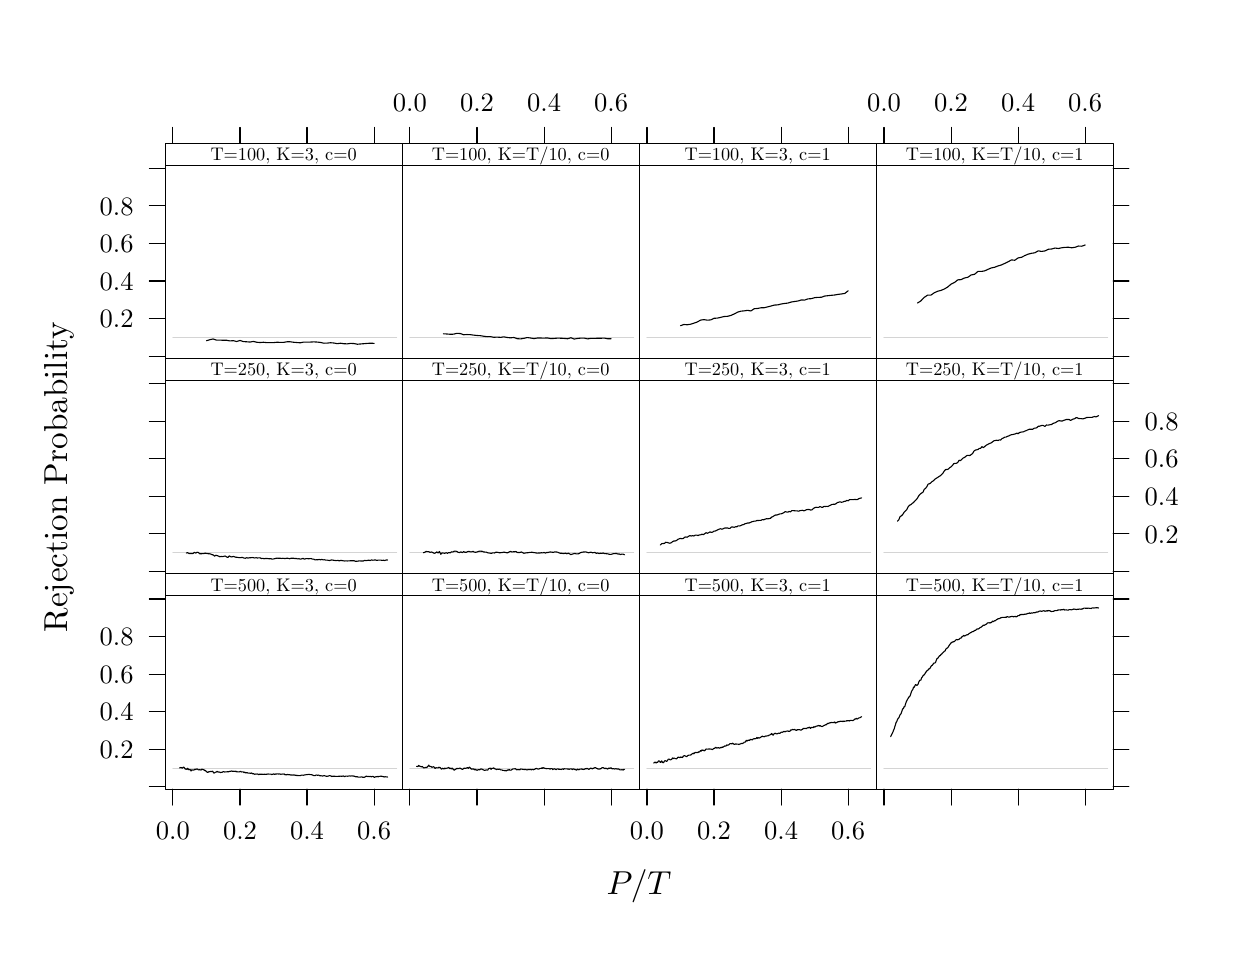
\begin{tikzpicture}[x=1pt,y=1pt]
\definecolor[named]{fillColor}{rgb}{1.00,1.00,1.00}
\path[use as bounding box,fill=fillColor,fill opacity=0.00] (0,0) rectangle (433.62,325.21);
\begin{scope}
\path[clip] (  0.00,  0.00) rectangle (433.62,325.21);

\path[] (  0.00,  0.00) rectangle (433.62,325.21);
\definecolor[named]{drawColor}{rgb}{0.00,0.00,0.00}

\node[text=drawColor,anchor=base,inner sep=0pt, outer sep=0pt, scale=  1.20] at (220.94, 12.05) {$P/T$};
\end{scope}
\begin{scope}
\path[clip] (  0.00,  0.00) rectangle (433.62,325.21);
\definecolor[named]{drawColor}{rgb}{0.00,0.00,0.00}

\node[text=drawColor,rotate= 90.00,anchor=base,inner sep=0pt, outer sep=0pt, scale=  1.20] at ( 14.29,162.76) {Rejection Probability};
\end{scope}
\begin{scope}
\path[clip] (  0.00,  0.00) rectangle (433.62,325.21);
\definecolor[named]{drawColor}{rgb}{0.00,0.00,0.00}

\path[draw=drawColor,line width= 0.4pt,line join=round,line cap=round] ( 49.65, 50.88) -- ( 43.95, 50.88);

\path[draw=drawColor,line width= 0.4pt,line join=round,line cap=round] ( 49.65, 64.45) -- ( 43.95, 64.45);

\path[draw=drawColor,line width= 0.4pt,line join=round,line cap=round] ( 49.65, 78.03) -- ( 43.95, 78.03);

\path[draw=drawColor,line width= 0.4pt,line join=round,line cap=round] ( 49.65, 91.61) -- ( 43.95, 91.61);

\path[draw=drawColor,line width= 0.4pt,line join=round,line cap=round] ( 49.65,105.18) -- ( 43.95,105.18);

\path[draw=drawColor,line width= 0.4pt,line join=round,line cap=round] ( 49.65,118.76) -- ( 43.95,118.76);

\node[text=drawColor,anchor=base east,inner sep=0pt, outer sep=0pt, scale=  0.96] at ( 38.26, 61.15) {0.2};

\node[text=drawColor,anchor=base east,inner sep=0pt, outer sep=0pt, scale=  0.96] at ( 38.26, 74.72) {0.4};

\node[text=drawColor,anchor=base east,inner sep=0pt, outer sep=0pt, scale=  0.96] at ( 38.26, 88.30) {0.6};

\node[text=drawColor,anchor=base east,inner sep=0pt, outer sep=0pt, scale=  0.96] at ( 38.26,101.88) {0.8};
\end{scope}
\begin{scope}
\path[clip] (  0.00,  0.00) rectangle (433.62,325.21);
\definecolor[named]{drawColor}{rgb}{0.00,0.00,0.00}

\path[draw=drawColor,line width= 0.4pt,line join=round,line cap=round] ( 52.48, 50.02) -- ( 52.48, 44.32);

\path[draw=drawColor,line width= 0.4pt,line join=round,line cap=round] ( 76.72, 50.02) -- ( 76.72, 44.32);

\path[draw=drawColor,line width= 0.4pt,line join=round,line cap=round] (100.95, 50.02) -- (100.95, 44.32);

\path[draw=drawColor,line width= 0.4pt,line join=round,line cap=round] (125.19, 50.02) -- (125.19, 44.32);

\node[text=drawColor,anchor=base,inner sep=0pt, outer sep=0pt, scale=  0.96] at ( 52.48, 32.02) {0.0};

\node[text=drawColor,anchor=base,inner sep=0pt, outer sep=0pt, scale=  0.96] at ( 76.72, 32.02) {0.2};

\node[text=drawColor,anchor=base,inner sep=0pt, outer sep=0pt, scale=  0.96] at (100.95, 32.02) {0.4};

\node[text=drawColor,anchor=base,inner sep=0pt, outer sep=0pt, scale=  0.96] at (125.19, 32.02) {0.6};
\end{scope}
\begin{scope}
\path[clip] ( 49.65, 50.02) rectangle (135.29,119.88);
\definecolor[named]{drawColor}{rgb}{0.83,0.83,0.83}

\path[draw=drawColor,line width= 0.4pt,line join=round,line cap=round] ( 52.48, 57.67) --
	(133.27, 57.67);
\definecolor[named]{drawColor}{rgb}{0.00,0.00,0.00}

\path[draw=drawColor,line width= 0.4pt,line join=round,line cap=round] ( 54.90, 57.73) --
	( 55.15, 57.80) --
	( 55.39, 57.87) --
	( 55.63, 57.77) --
	( 55.87, 57.60) --
	( 56.12, 57.90) --
	( 56.36, 58.01) --
	( 56.60, 57.80) --
	( 56.84, 57.43) --
	( 57.09, 57.22) --
	( 57.33, 57.39) --
	( 57.57, 57.16) --
	( 57.81, 57.60) --
	( 58.05, 57.26) --
	( 58.30, 57.02) --
	( 58.54, 57.16) --
	( 58.78, 57.12) --
	( 59.02, 56.61) --
	( 59.27, 57.05) --
	( 59.51, 56.95) --
	( 59.75, 56.99) --
	( 59.99, 56.95) --
	( 60.24, 57.05) --
	( 60.48, 57.29) --
	( 60.72, 57.12) --
	( 60.96, 57.29) --
	( 61.21, 57.36) --
	( 61.45, 57.22) --
	( 61.69, 57.02) --
	( 61.93, 57.02) --
	( 62.17, 57.09) --
	( 62.42, 57.02) --
	( 62.66, 56.92) --
	( 62.90, 57.26) --
	( 63.14, 57.22) --
	( 63.39, 57.12) --
	( 63.63, 57.09) --
	( 63.87, 56.75) --
	( 64.11, 56.89) --
	( 64.36, 56.55) --
	( 64.60, 56.55) --
	( 64.84, 56.17) --
	( 65.08, 56.07) --
	( 65.33, 56.27) --
	( 65.57, 56.41) --
	( 65.81, 56.34) --
	( 66.05, 56.48) --
	( 66.29, 56.38) --
	( 66.54, 56.44) --
	( 66.78, 56.55) --
	( 67.02, 56.24) --
	( 67.26, 55.87) --
	( 67.51, 55.93) --
	( 67.75, 56.10) --
	( 67.99, 56.21) --
	( 68.23, 56.27) --
	( 68.48, 56.48) --
	( 68.72, 56.24) --
	( 68.96, 56.27) --
	( 69.20, 56.24) --
	( 69.45, 56.17) --
	( 69.69, 56.04) --
	( 69.93, 56.14) --
	( 70.17, 56.10) --
	( 70.41, 56.24) --
	( 70.66, 56.38) --
	( 70.90, 56.34) --
	( 71.14, 56.24) --
	( 71.38, 56.27) --
	( 71.63, 56.27) --
	( 71.87, 56.27) --
	( 72.11, 56.34) --
	( 72.35, 56.31) --
	( 72.60, 56.34) --
	( 72.84, 56.41) --
	( 73.08, 56.51) --
	( 73.32, 56.48) --
	( 73.57, 56.61) --
	( 73.81, 56.55) --
	( 74.05, 56.51) --
	( 74.29, 56.51) --
	( 74.53, 56.48) --
	( 74.78, 56.48) --
	( 75.02, 56.58) --
	( 75.26, 56.31) --
	( 75.50, 56.48) --
	( 75.75, 56.31) --
	( 75.99, 56.31) --
	( 76.23, 56.27) --
	( 76.47, 56.31) --
	( 76.72, 56.38) --
	( 76.96, 56.51) --
	( 77.20, 56.24) --
	( 77.44, 56.31) --
	( 77.69, 56.27) --
	( 77.93, 56.27) --
	( 78.17, 56.00) --
	( 78.41, 56.21) --
	( 78.66, 55.97) --
	( 78.90, 56.00) --
	( 79.14, 55.93) --
	( 79.38, 56.00) --
	( 79.62, 55.83) --
	( 79.87, 55.83) --
	( 80.11, 55.87) --
	( 80.35, 55.80) --
	( 80.59, 55.77) --
	( 80.84, 55.90) --
	( 81.08, 55.77) --
	( 81.32, 55.60) --
	( 81.56, 55.66) --
	( 81.81, 55.53) --
	( 82.05, 55.43) --
	( 82.29, 55.49) --
	( 82.53, 55.53) --
	( 82.78, 55.46) --
	( 83.02, 55.53) --
	( 83.26, 55.46) --
	( 83.50, 55.26) --
	( 83.74, 55.46) --
	( 83.99, 55.43) --
	( 84.23, 55.43) --
	( 84.47, 55.43) --
	( 84.71, 55.39) --
	( 84.96, 55.43) --
	( 85.20, 55.39) --
	( 85.44, 55.43) --
	( 85.68, 55.43) --
	( 85.93, 55.36) --
	( 86.17, 55.43) --
	( 86.41, 55.43) --
	( 86.65, 55.49) --
	( 86.90, 55.53) --
	( 87.14, 55.49) --
	( 87.38, 55.46) --
	( 87.62, 55.46) --
	( 87.86, 55.49) --
	( 88.11, 55.36) --
	( 88.35, 55.36) --
	( 88.59, 55.43) --
	( 88.83, 55.60) --
	( 89.08, 55.46) --
	( 89.32, 55.36) --
	( 89.56, 55.53) --
	( 89.80, 55.53) --
	( 90.05, 55.53) --
	( 90.29, 55.60) --
	( 90.53, 55.53) --
	( 90.77, 55.53) --
	( 91.02, 55.56) --
	( 91.26, 55.46) --
	( 91.50, 55.43) --
	( 91.74, 55.46) --
	( 91.98, 55.46) --
	( 92.23, 55.53) --
	( 92.47, 55.46) --
	( 92.71, 55.56) --
	( 92.95, 55.26) --
	( 93.20, 55.29) --
	( 93.44, 55.22) --
	( 93.68, 55.26) --
	( 93.92, 55.36) --
	( 94.17, 55.29) --
	( 94.41, 55.26) --
	( 94.65, 55.29) --
	( 94.89, 55.19) --
	( 95.14, 55.15) --
	( 95.38, 55.15) --
	( 95.62, 55.12) --
	( 95.86, 55.22) --
	( 96.10, 55.15) --
	( 96.35, 55.19) --
	( 96.59, 55.09) --
	( 96.83, 55.09) --
	( 97.07, 55.05) --
	( 97.32, 54.92) --
	( 97.56, 55.02) --
	( 97.80, 54.95) --
	( 98.04, 54.95) --
	( 98.29, 54.95) --
	( 98.53, 54.95) --
	( 98.77, 55.05) --
	( 99.01, 55.12) --
	( 99.26, 55.12) --
	( 99.50, 55.09) --
	( 99.74, 55.09) --
	( 99.98, 55.15) --
	(100.22, 55.22) --
	(100.47, 55.22) --
	(100.71, 55.32) --
	(100.95, 55.32) --
	(101.19, 55.32) --
	(101.44, 55.39) --
	(101.68, 55.39) --
	(101.92, 55.32) --
	(102.16, 55.32) --
	(102.41, 55.32) --
	(102.65, 55.22) --
	(102.89, 55.19) --
	(103.13, 55.05) --
	(103.38, 54.98) --
	(103.62, 54.92) --
	(103.86, 54.92) --
	(104.10, 55.09) --
	(104.34, 55.15) --
	(104.59, 55.09) --
	(104.83, 55.09) --
	(105.07, 55.15) --
	(105.31, 55.02) --
	(105.56, 54.88) --
	(105.80, 54.88) --
	(106.04, 54.88) --
	(106.28, 54.85) --
	(106.53, 54.78) --
	(106.77, 54.85) --
	(107.01, 54.92) --
	(107.25, 54.92) --
	(107.50, 54.81) --
	(107.74, 54.75) --
	(107.98, 54.71) --
	(108.22, 54.68) --
	(108.46, 54.75) --
	(108.71, 54.78) --
	(108.95, 54.92) --
	(109.19, 54.95) --
	(109.43, 54.85) --
	(109.68, 54.78) --
	(109.92, 54.61) --
	(110.16, 54.71) --
	(110.40, 54.71) --
	(110.65, 54.68) --
	(110.89, 54.75) --
	(111.13, 54.68) --
	(111.37, 54.64) --
	(111.62, 54.64) --
	(111.86, 54.64) --
	(112.10, 54.64) --
	(112.34, 54.71) --
	(112.58, 54.68) --
	(112.83, 54.71) --
	(113.07, 54.78) --
	(113.31, 54.68) --
	(113.55, 54.71) --
	(113.80, 54.75) --
	(114.04, 54.81) --
	(114.28, 54.68) --
	(114.52, 54.58) --
	(114.77, 54.71) --
	(115.01, 54.78) --
	(115.25, 54.78) --
	(115.49, 54.71) --
	(115.74, 54.75) --
	(115.98, 54.78) --
	(116.22, 54.85) --
	(116.46, 54.85) --
	(116.70, 54.71) --
	(116.95, 54.85) --
	(117.19, 54.85) --
	(117.43, 54.81) --
	(117.67, 54.81) --
	(117.92, 54.71) --
	(118.16, 54.71) --
	(118.40, 54.54) --
	(118.64, 54.54) --
	(118.89, 54.54) --
	(119.13, 54.54) --
	(119.37, 54.41) --
	(119.61, 54.37) --
	(119.86, 54.41) --
	(120.10, 54.37) --
	(120.34, 54.41) --
	(120.58, 54.48) --
	(120.83, 54.48) --
	(121.07, 54.34) --
	(121.31, 54.34) --
	(121.55, 54.31) --
	(121.79, 54.41) --
	(122.04, 54.54) --
	(122.28, 54.71) --
	(122.52, 54.71) --
	(122.76, 54.64) --
	(123.01, 54.61) --
	(123.25, 54.68) --
	(123.49, 54.58) --
	(123.73, 54.61) --
	(123.98, 54.61) --
	(124.22, 54.51) --
	(124.46, 54.61) --
	(124.70, 54.68) --
	(124.95, 54.58) --
	(125.19, 54.31) --
	(125.43, 54.37) --
	(125.67, 54.48) --
	(125.91, 54.58) --
	(126.16, 54.54) --
	(126.40, 54.64) --
	(126.64, 54.44) --
	(126.88, 54.68) --
	(127.13, 54.68) --
	(127.37, 54.68) --
	(127.61, 54.75) --
	(127.85, 54.71) --
	(128.10, 54.68) --
	(128.34, 54.61) --
	(128.58, 54.54) --
	(128.82, 54.44) --
	(129.07, 54.54) --
	(129.31, 54.51) --
	(129.55, 54.48) --
	(129.79, 54.48) --
	(130.03, 54.41);
\end{scope}
\begin{scope}
\path[clip] (  0.00,  0.00) rectangle (433.62,325.21);
\definecolor[named]{drawColor}{rgb}{0.00,0.00,0.00}

\path[draw=drawColor,line width= 0.4pt,line join=round,line cap=round] ( 49.65, 50.02) rectangle (135.29,119.88);
\end{scope}
\begin{scope}
\path[clip] ( 49.65,119.88) rectangle (135.29,127.83);

\path[] ( 49.65,119.88) rectangle (135.29,127.83);
\definecolor[named]{drawColor}{rgb}{0.00,0.00,0.00}

\node[text=drawColor,anchor=base west,inner sep=0pt, outer sep=0pt, scale=  0.66] at ( 66.08,121.58) {T=500, K=3, c=0};
\end{scope}
\begin{scope}
\path[clip] (  0.00,  0.00) rectangle (433.62,325.21);
\definecolor[named]{drawColor}{rgb}{0.00,0.00,0.00}

\path[draw=drawColor,line width= 0.4pt,line join=round,line cap=round] ( 49.65,119.88) rectangle (135.29,127.83);
\end{scope}
\begin{scope}
\path[clip] (  0.00,  0.00) rectangle (433.62,325.21);
\definecolor[named]{drawColor}{rgb}{0.00,0.00,0.00}

\path[draw=drawColor,line width= 0.4pt,line join=round,line cap=round] (138.13, 50.02) -- (138.13, 44.32);

\path[draw=drawColor,line width= 0.4pt,line join=round,line cap=round] (162.36, 50.02) -- (162.36, 44.32);

\path[draw=drawColor,line width= 0.4pt,line join=round,line cap=round] (186.60, 50.02) -- (186.60, 44.32);

\path[draw=drawColor,line width= 0.4pt,line join=round,line cap=round] (210.84, 50.02) -- (210.84, 44.32);
\end{scope}
\begin{scope}
\path[clip] (135.29, 50.02) rectangle (220.94,119.88);
\definecolor[named]{drawColor}{rgb}{0.83,0.83,0.83}

\path[draw=drawColor,line width= 0.4pt,line join=round,line cap=round] (138.13, 57.67) --
	(218.91, 57.67);
\definecolor[named]{drawColor}{rgb}{0.00,0.00,0.00}

\path[draw=drawColor,line width= 0.4pt,line join=round,line cap=round] (140.55, 58.28) --
	(140.80, 58.24) --
	(141.04, 58.28) --
	(141.28, 58.62) --
	(141.52, 58.38) --
	(141.76, 58.31) --
	(142.01, 58.21) --
	(142.25, 58.07) --
	(142.49, 58.24) --
	(142.73, 58.17) --
	(142.98, 57.73) --
	(143.22, 57.80) --
	(143.46, 57.73) --
	(143.70, 57.84) --
	(143.95, 57.97) --
	(144.19, 57.80) --
	(144.43, 58.14) --
	(144.67, 58.31) --
	(144.92, 58.72) --
	(145.16, 58.38) --
	(145.40, 58.21) --
	(145.64, 58.28) --
	(145.88, 58.11) --
	(146.13, 57.94) --
	(146.37, 58.07) --
	(146.61, 58.14) --
	(146.85, 58.04) --
	(147.10, 57.63) --
	(147.34, 57.60) --
	(147.58, 57.80) --
	(147.82, 57.73) --
	(148.07, 57.73) --
	(148.31, 57.73) --
	(148.55, 57.97) --
	(148.79, 57.84) --
	(149.04, 57.87) --
	(149.28, 57.60) --
	(149.52, 57.26) --
	(149.76, 57.43) --
	(150.00, 57.63) --
	(150.25, 57.36) --
	(150.49, 57.36) --
	(150.73, 57.67) --
	(150.97, 57.46) --
	(151.22, 57.53) --
	(151.46, 57.67) --
	(151.70, 57.67) --
	(151.94, 57.80) --
	(152.19, 57.90) --
	(152.43, 57.53) --
	(152.67, 57.46) --
	(152.91, 57.63) --
	(153.16, 57.39) --
	(153.40, 57.67) --
	(153.64, 57.36) --
	(153.88, 57.16) --
	(154.12, 56.89) --
	(154.37, 57.05) --
	(154.61, 57.26) --
	(154.85, 57.33) --
	(155.09, 57.63) --
	(155.34, 57.43) --
	(155.58, 57.50) --
	(155.82, 57.46) --
	(156.06, 57.63) --
	(156.31, 57.63) --
	(156.55, 57.46) --
	(156.79, 57.36) --
	(157.03, 57.22) --
	(157.28, 57.26) --
	(157.52, 57.50) --
	(157.76, 57.70) --
	(158.00, 57.53) --
	(158.24, 57.60) --
	(158.49, 57.63) --
	(158.73, 57.77) --
	(158.97, 57.80) --
	(159.21, 57.53) --
	(159.46, 57.87) --
	(159.70, 58.01) --
	(159.94, 57.67) --
	(160.18, 57.43) --
	(160.43, 57.22) --
	(160.67, 57.39) --
	(160.91, 57.33) --
	(161.15, 57.33) --
	(161.40, 57.05) --
	(161.64, 57.29) --
	(161.88, 56.99) --
	(162.12, 57.05) --
	(162.36, 56.85) --
	(162.61, 56.99) --
	(162.85, 57.09) --
	(163.09, 57.09) --
	(163.33, 56.99) --
	(163.58, 57.22) --
	(163.82, 57.36) --
	(164.06, 57.29) --
	(164.30, 57.22) --
	(164.55, 57.05) --
	(164.79, 56.99) --
	(165.03, 56.82) --
	(165.27, 56.85) --
	(165.52, 56.95) --
	(165.76, 57.02) --
	(166.00, 56.92) --
	(166.24, 56.92) --
	(166.48, 57.36) --
	(166.73, 57.50) --
	(166.97, 57.60) --
	(167.21, 57.60) --
	(167.45, 57.19) --
	(167.70, 57.60) --
	(167.94, 57.56) --
	(168.18, 57.60) --
	(168.42, 57.77) --
	(168.67, 57.43) --
	(168.91, 57.39) --
	(169.15, 57.29) --
	(169.39, 57.12) --
	(169.64, 57.29) --
	(169.88, 57.26) --
	(170.12, 57.16) --
	(170.36, 57.29) --
	(170.60, 57.26) --
	(170.85, 57.05) --
	(171.09, 56.99) --
	(171.33, 57.02) --
	(171.57, 56.85) --
	(171.82, 56.85) --
	(172.06, 56.82) --
	(172.30, 56.78) --
	(172.54, 56.65) --
	(172.79, 56.85) --
	(173.03, 56.68) --
	(173.27, 56.85) --
	(173.51, 57.02) --
	(173.76, 56.95) --
	(174.00, 57.16) --
	(174.24, 56.89) --
	(174.48, 56.95) --
	(174.73, 56.92) --
	(174.97, 57.12) --
	(175.21, 57.29) --
	(175.45, 57.36) --
	(175.69, 57.39) --
	(175.94, 57.39) --
	(176.18, 57.46) --
	(176.42, 57.29) --
	(176.66, 57.05) --
	(176.91, 57.12) --
	(177.15, 57.05) --
	(177.39, 57.09) --
	(177.63, 57.09) --
	(177.88, 57.02) --
	(178.12, 57.36) --
	(178.36, 57.26) --
	(178.60, 57.29) --
	(178.85, 57.22) --
	(179.09, 57.19) --
	(179.33, 57.16) --
	(179.57, 57.16) --
	(179.81, 57.19) --
	(180.06, 57.12) --
	(180.30, 56.99) --
	(180.54, 56.99) --
	(180.78, 57.16) --
	(181.03, 57.12) --
	(181.27, 57.09) --
	(181.51, 57.19) --
	(181.75, 57.16) --
	(182.00, 56.99) --
	(182.24, 57.22) --
	(182.48, 57.16) --
	(182.72, 57.05) --
	(182.97, 57.16) --
	(183.21, 57.22) --
	(183.45, 57.43) --
	(183.69, 57.50) --
	(183.93, 57.50) --
	(184.18, 57.39) --
	(184.42, 57.29) --
	(184.66, 57.29) --
	(184.90, 57.43) --
	(185.15, 57.56) --
	(185.39, 57.56) --
	(185.63, 57.53) --
	(185.87, 57.80) --
	(186.12, 57.56) --
	(186.36, 57.80) --
	(186.60, 57.73) --
	(186.84, 57.56) --
	(187.09, 57.53) --
	(187.33, 57.43) --
	(187.57, 57.50) --
	(187.81, 57.46) --
	(188.05, 57.46) --
	(188.30, 57.46) --
	(188.54, 57.43) --
	(188.78, 57.29) --
	(189.02, 57.46) --
	(189.27, 57.46) --
	(189.51, 57.46) --
	(189.75, 57.09) --
	(189.99, 57.33) --
	(190.24, 57.33) --
	(190.48, 57.43) --
	(190.72, 57.22) --
	(190.96, 57.12) --
	(191.21, 57.29) --
	(191.45, 57.39) --
	(191.69, 57.39) --
	(191.93, 57.22) --
	(192.17, 57.29) --
	(192.42, 57.19) --
	(192.66, 57.19) --
	(192.90, 57.16) --
	(193.14, 57.33) --
	(193.39, 57.39) --
	(193.63, 57.19) --
	(193.87, 57.43) --
	(194.11, 57.39) --
	(194.36, 57.36) --
	(194.60, 57.36) --
	(194.84, 57.36) --
	(195.08, 57.33) --
	(195.33, 57.36) --
	(195.57, 57.22) --
	(195.81, 57.26) --
	(196.05, 57.39) --
	(196.29, 57.39) --
	(196.54, 57.39) --
	(196.78, 57.12) --
	(197.02, 57.26) --
	(197.26, 57.43) --
	(197.51, 57.26) --
	(197.75, 57.12) --
	(197.99, 57.16) --
	(198.23, 56.89) --
	(198.48, 57.05) --
	(198.72, 57.29) --
	(198.96, 57.12) --
	(199.20, 57.05) --
	(199.45, 57.26) --
	(199.69, 57.29) --
	(199.93, 57.29) --
	(200.17, 57.39) --
	(200.41, 57.22) --
	(200.66, 57.26) --
	(200.90, 57.16) --
	(201.14, 57.22) --
	(201.38, 57.39) --
	(201.63, 57.43) --
	(201.87, 57.39) --
	(202.11, 57.60) --
	(202.35, 57.46) --
	(202.60, 57.26) --
	(202.84, 57.22) --
	(203.08, 57.39) --
	(203.32, 57.60) --
	(203.57, 57.63) --
	(203.81, 57.50) --
	(204.05, 57.36) --
	(204.29, 57.60) --
	(204.53, 57.60) --
	(204.78, 57.73) --
	(205.02, 57.84) --
	(205.26, 57.77) --
	(205.50, 57.60) --
	(205.75, 57.53) --
	(205.99, 57.36) --
	(206.23, 57.33) --
	(206.47, 57.36) --
	(206.72, 57.26) --
	(206.96, 57.43) --
	(207.20, 57.46) --
	(207.44, 57.73) --
	(207.69, 57.84) --
	(207.93, 57.84) --
	(208.17, 57.70) --
	(208.41, 57.53) --
	(208.65, 57.46) --
	(208.90, 57.63) --
	(209.14, 57.53) --
	(209.38, 57.39) --
	(209.62, 57.33) --
	(209.87, 57.60) --
	(210.11, 57.70) --
	(210.35, 57.50) --
	(210.59, 57.70) --
	(210.84, 57.73) --
	(211.08, 57.46) --
	(211.32, 57.39) --
	(211.56, 57.46) --
	(211.81, 57.43) --
	(212.05, 57.33) --
	(212.29, 57.36) --
	(212.53, 57.46) --
	(212.77, 57.36) --
	(213.02, 57.29) --
	(213.26, 57.36) --
	(213.50, 57.33) --
	(213.74, 57.22) --
	(213.99, 57.05) --
	(214.23, 57.02) --
	(214.47, 56.99) --
	(214.71, 57.12) --
	(214.96, 57.05) --
	(215.20, 56.95) --
	(215.44, 57.22) --
	(215.68, 57.19);
\end{scope}
\begin{scope}
\path[clip] (  0.00,  0.00) rectangle (433.62,325.21);
\definecolor[named]{drawColor}{rgb}{0.00,0.00,0.00}

\path[draw=drawColor,line width= 0.4pt,line join=round,line cap=round] (135.29, 50.02) rectangle (220.94,119.88);
\end{scope}
\begin{scope}
\path[clip] (135.29,119.88) rectangle (220.94,127.83);

\path[] (135.29,119.88) rectangle (220.94,127.83);
\definecolor[named]{drawColor}{rgb}{0.00,0.00,0.00}

\node[text=drawColor,anchor=base west,inner sep=0pt, outer sep=0pt, scale=  0.66] at (146.04,121.58) {T=500, K=T/10, c=0};
\end{scope}
\begin{scope}
\path[clip] (  0.00,  0.00) rectangle (433.62,325.21);
\definecolor[named]{drawColor}{rgb}{0.00,0.00,0.00}

\path[draw=drawColor,line width= 0.4pt,line join=round,line cap=round] (135.29,119.88) rectangle (220.94,127.83);
\end{scope}
\begin{scope}
\path[clip] (  0.00,  0.00) rectangle (433.62,325.21);
\definecolor[named]{drawColor}{rgb}{0.00,0.00,0.00}

\path[draw=drawColor,line width= 0.4pt,line join=round,line cap=round] (223.78, 50.02) -- (223.78, 44.32);

\path[draw=drawColor,line width= 0.4pt,line join=round,line cap=round] (248.01, 50.02) -- (248.01, 44.32);

\path[draw=drawColor,line width= 0.4pt,line join=round,line cap=round] (272.25, 50.02) -- (272.25, 44.32);

\path[draw=drawColor,line width= 0.4pt,line join=round,line cap=round] (296.48, 50.02) -- (296.48, 44.32);

\node[text=drawColor,anchor=base,inner sep=0pt, outer sep=0pt, scale=  0.96] at (223.78, 32.02) {0.0};

\node[text=drawColor,anchor=base,inner sep=0pt, outer sep=0pt, scale=  0.96] at (248.01, 32.02) {0.2};

\node[text=drawColor,anchor=base,inner sep=0pt, outer sep=0pt, scale=  0.96] at (272.25, 32.02) {0.4};

\node[text=drawColor,anchor=base,inner sep=0pt, outer sep=0pt, scale=  0.96] at (296.48, 32.02) {0.6};
\end{scope}
\begin{scope}
\path[clip] (220.94, 50.02) rectangle (306.59,119.88);
\definecolor[named]{drawColor}{rgb}{0.83,0.83,0.83}

\path[draw=drawColor,line width= 0.4pt,line join=round,line cap=round] (223.78, 57.67) --
	(304.56, 57.67);
\definecolor[named]{drawColor}{rgb}{0.00,0.00,0.00}

\path[draw=drawColor,line width= 0.4pt,line join=round,line cap=round] (226.20, 59.50) --
	(226.44, 59.63) --
	(226.69, 59.84) --
	(226.93, 59.60) --
	(227.17, 59.53) --
	(227.41, 59.84) --
	(227.66, 59.74) --
	(227.90, 60.21) --
	(228.14, 60.28) --
	(228.38, 60.08) --
	(228.62, 59.70) --
	(228.87, 59.87) --
	(229.11, 60.25) --
	(229.35, 59.80) --
	(229.59, 59.57) --
	(229.84, 59.74) --
	(230.08, 60.18) --
	(230.32, 60.35) --
	(230.56, 60.25) --
	(230.81, 60.11) --
	(231.05, 60.18) --
	(231.29, 60.58) --
	(231.53, 60.92) --
	(231.78, 60.92) --
	(232.02, 60.72) --
	(232.26, 60.58) --
	(232.50, 60.75) --
	(232.75, 60.89) --
	(232.99, 61.33) --
	(233.23, 61.06) --
	(233.47, 61.26) --
	(233.71, 61.23) --
	(233.96, 61.06) --
	(234.20, 61.09) --
	(234.44, 60.99) --
	(234.68, 61.23) --
	(234.93, 61.57) --
	(235.17, 61.57) --
	(235.41, 61.53) --
	(235.65, 61.43) --
	(235.90, 61.67) --
	(236.14, 61.57) --
	(236.38, 61.57) --
	(236.62, 61.47) --
	(236.87, 61.98) --
	(237.11, 62.08) --
	(237.35, 62.15) --
	(237.59, 62.04) --
	(237.83, 61.94) --
	(238.08, 61.77) --
	(238.32, 61.94) --
	(238.56, 62.21) --
	(238.80, 62.28) --
	(239.05, 62.35) --
	(239.29, 62.32) --
	(239.53, 62.32) --
	(239.77, 62.55) --
	(240.02, 62.79) --
	(240.26, 62.86) --
	(240.50, 63.06) --
	(240.74, 62.82) --
	(240.99, 63.16) --
	(241.23, 63.33) --
	(241.47, 63.23) --
	(241.71, 63.30) --
	(241.95, 63.33) --
	(242.20, 63.20) --
	(242.44, 63.57) --
	(242.68, 63.44) --
	(242.92, 63.71) --
	(243.17, 63.98) --
	(243.41, 63.81) --
	(243.65, 64.22) --
	(243.89, 64.05) --
	(244.14, 64.15) --
	(244.38, 63.94) --
	(244.62, 63.94) --
	(244.86, 64.22) --
	(245.11, 64.56) --
	(245.35, 64.49) --
	(245.59, 64.52) --
	(245.83, 64.49) --
	(246.07, 64.56) --
	(246.32, 64.56) --
	(246.56, 64.56) --
	(246.80, 64.52) --
	(247.04, 64.52) --
	(247.29, 64.39) --
	(247.53, 64.39) --
	(247.77, 64.66) --
	(248.01, 64.79) --
	(248.26, 64.79) --
	(248.50, 65.17) --
	(248.74, 65.13) --
	(248.98, 64.86) --
	(249.23, 64.96) --
	(249.47, 65.03) --
	(249.71, 65.00) --
	(249.95, 64.83) --
	(250.19, 64.93) --
	(250.44, 65.13) --
	(250.68, 65.00) --
	(250.92, 65.30) --
	(251.16, 65.17) --
	(251.41, 65.34) --
	(251.65, 65.51) --
	(251.89, 65.68) --
	(252.13, 65.57) --
	(252.38, 65.68) --
	(252.62, 66.05) --
	(252.86, 65.91) --
	(253.10, 65.98) --
	(253.35, 66.08) --
	(253.59, 66.32) --
	(253.83, 66.49) --
	(254.07, 66.49) --
	(254.31, 66.39) --
	(254.56, 66.52) --
	(254.80, 66.66) --
	(255.04, 66.35) --
	(255.28, 66.29) --
	(255.53, 66.22) --
	(255.77, 66.39) --
	(256.01, 66.39) --
	(256.25, 66.29) --
	(256.50, 66.32) --
	(256.74, 66.29) --
	(256.98, 66.18) --
	(257.22, 66.29) --
	(257.47, 66.39) --
	(257.71, 66.46) --
	(257.95, 66.63) --
	(258.19, 66.52) --
	(258.43, 66.66) --
	(258.68, 66.69) --
	(258.92, 67.03) --
	(259.16, 67.03) --
	(259.40, 67.10) --
	(259.65, 67.71) --
	(259.89, 67.41) --
	(260.13, 67.58) --
	(260.37, 67.78) --
	(260.62, 67.71) --
	(260.86, 67.64) --
	(261.10, 68.05) --
	(261.34, 68.02) --
	(261.59, 67.95) --
	(261.83, 67.81) --
	(262.07, 68.12) --
	(262.31, 68.25) --
	(262.55, 68.25) --
	(262.80, 68.25) --
	(263.04, 68.32) --
	(263.28, 68.39) --
	(263.52, 68.73) --
	(263.77, 68.42) --
	(264.01, 68.66) --
	(264.25, 68.49) --
	(264.49, 68.56) --
	(264.74, 68.73) --
	(264.98, 68.87) --
	(265.22, 69.04) --
	(265.46, 69.24) --
	(265.71, 69.00) --
	(265.95, 69.04) --
	(266.19, 69.00) --
	(266.43, 69.14) --
	(266.67, 69.24) --
	(266.92, 69.21) --
	(267.16, 69.34) --
	(267.40, 69.27) --
	(267.64, 69.38) --
	(267.89, 69.58) --
	(268.13, 69.58) --
	(268.37, 69.78) --
	(268.61, 69.88) --
	(268.86, 70.16) --
	(269.10, 69.85) --
	(269.34, 69.54) --
	(269.58, 69.95) --
	(269.83, 70.05) --
	(270.07, 70.26) --
	(270.31, 70.19) --
	(270.55, 70.02) --
	(270.79, 70.05) --
	(271.04, 70.12) --
	(271.28, 70.29) --
	(271.52, 70.29) --
	(271.76, 70.19) --
	(272.01, 70.36) --
	(272.25, 70.60) --
	(272.49, 70.66) --
	(272.73, 70.60) --
	(272.98, 70.73) --
	(273.22, 70.94) --
	(273.46, 70.87) --
	(273.70, 70.77) --
	(273.95, 70.90) --
	(274.19, 71.04) --
	(274.43, 71.00) --
	(274.67, 71.07) --
	(274.92, 70.97) --
	(275.16, 70.94) --
	(275.40, 70.90) --
	(275.64, 71.34) --
	(275.88, 71.48) --
	(276.13, 71.41) --
	(276.37, 71.65) --
	(276.61, 71.51) --
	(276.85, 71.58) --
	(277.10, 71.68) --
	(277.34, 71.45) --
	(277.58, 71.38) --
	(277.82, 71.24) --
	(278.07, 71.55) --
	(278.31, 71.48) --
	(278.55, 71.58) --
	(278.79, 71.55) --
	(279.04, 71.48) --
	(279.28, 71.41) --
	(279.52, 71.41) --
	(279.76, 71.58) --
	(280.00, 71.65) --
	(280.25, 72.02) --
	(280.49, 71.92) --
	(280.73, 71.99) --
	(280.97, 71.99) --
	(281.22, 71.95) --
	(281.46, 71.92) --
	(281.70, 72.19) --
	(281.94, 72.23) --
	(282.19, 72.23) --
	(282.43, 72.46) --
	(282.67, 72.23) --
	(282.91, 71.99) --
	(283.16, 72.40) --
	(283.40, 72.36) --
	(283.64, 72.33) --
	(283.88, 72.26) --
	(284.12, 72.67) --
	(284.37, 72.46) --
	(284.61, 72.60) --
	(284.85, 72.74) --
	(285.09, 72.84) --
	(285.34, 72.87) --
	(285.58, 72.97) --
	(285.82, 73.07) --
	(286.06, 72.84) --
	(286.31, 73.01) --
	(286.55, 72.87) --
	(286.79, 72.74) --
	(287.03, 72.67) --
	(287.28, 72.77) --
	(287.52, 72.90) --
	(287.76, 73.07) --
	(288.00, 73.14) --
	(288.24, 73.31) --
	(288.49, 73.31) --
	(288.73, 73.45) --
	(288.97, 73.82) --
	(289.21, 73.69) --
	(289.46, 73.89) --
	(289.70, 73.92) --
	(289.94, 74.06) --
	(290.18, 74.06) --
	(290.43, 74.19) --
	(290.67, 74.09) --
	(290.91, 74.09) --
	(291.15, 74.19) --
	(291.40, 74.09) --
	(291.64, 74.33) --
	(291.88, 73.92) --
	(292.12, 74.02) --
	(292.36, 74.16) --
	(292.61, 74.30) --
	(292.85, 74.47) --
	(293.09, 74.33) --
	(293.33, 74.53) --
	(293.58, 74.53) --
	(293.82, 74.60) --
	(294.06, 74.50) --
	(294.30, 74.60) --
	(294.55, 74.43) --
	(294.79, 74.70) --
	(295.03, 74.50) --
	(295.27, 74.64) --
	(295.52, 74.64) --
	(295.76, 74.64) --
	(296.00, 74.84) --
	(296.24, 74.74) --
	(296.48, 74.77) --
	(296.73, 74.84) --
	(296.97, 74.64) --
	(297.21, 74.91) --
	(297.45, 74.91) --
	(297.70, 74.91) --
	(297.94, 74.84) --
	(298.18, 74.81) --
	(298.42, 74.98) --
	(298.67, 75.14) --
	(298.91, 75.42) --
	(299.15, 75.35) --
	(299.39, 75.65) --
	(299.64, 75.38) --
	(299.88, 75.45) --
	(300.12, 75.65) --
	(300.36, 75.79) --
	(300.60, 75.82) --
	(300.85, 75.93) --
	(301.09, 76.10) --
	(301.33, 76.23);
\end{scope}
\begin{scope}
\path[clip] (  0.00,  0.00) rectangle (433.62,325.21);
\definecolor[named]{drawColor}{rgb}{0.00,0.00,0.00}

\path[draw=drawColor,line width= 0.4pt,line join=round,line cap=round] (220.94, 50.02) rectangle (306.59,119.88);
\end{scope}
\begin{scope}
\path[clip] (220.94,119.88) rectangle (306.59,127.83);

\path[] (220.94,119.88) rectangle (306.59,127.83);
\definecolor[named]{drawColor}{rgb}{0.00,0.00,0.00}

\node[text=drawColor,anchor=base west,inner sep=0pt, outer sep=0pt, scale=  0.66] at (237.37,121.58) {T=500, K=3, c=1};
\end{scope}
\begin{scope}
\path[clip] (  0.00,  0.00) rectangle (433.62,325.21);
\definecolor[named]{drawColor}{rgb}{0.00,0.00,0.00}

\path[draw=drawColor,line width= 0.4pt,line join=round,line cap=round] (220.94,119.88) rectangle (306.59,127.83);
\end{scope}
\begin{scope}
\path[clip] (  0.00,  0.00) rectangle (433.62,325.21);
\definecolor[named]{drawColor}{rgb}{0.00,0.00,0.00}

\path[draw=drawColor,line width= 0.4pt,line join=round,line cap=round] (309.43, 50.02) -- (309.43, 44.32);

\path[draw=drawColor,line width= 0.4pt,line join=round,line cap=round] (333.66, 50.02) -- (333.66, 44.32);

\path[draw=drawColor,line width= 0.4pt,line join=round,line cap=round] (357.90, 50.02) -- (357.90, 44.32);

\path[draw=drawColor,line width= 0.4pt,line join=round,line cap=round] (382.13, 50.02) -- (382.13, 44.32);

\path[draw=drawColor,line width= 0.4pt,line join=round,line cap=round] (392.24, 50.88) -- (397.93, 50.88);

\path[draw=drawColor,line width= 0.4pt,line join=round,line cap=round] (392.24, 64.45) -- (397.93, 64.45);

\path[draw=drawColor,line width= 0.4pt,line join=round,line cap=round] (392.24, 78.03) -- (397.93, 78.03);

\path[draw=drawColor,line width= 0.4pt,line join=round,line cap=round] (392.24, 91.61) -- (397.93, 91.61);

\path[draw=drawColor,line width= 0.4pt,line join=round,line cap=round] (392.24,105.18) -- (397.93,105.18);

\path[draw=drawColor,line width= 0.4pt,line join=round,line cap=round] (392.24,118.76) -- (397.93,118.76);
\end{scope}
\begin{scope}
\path[clip] (306.59, 50.02) rectangle (392.24,119.88);
\definecolor[named]{drawColor}{rgb}{0.83,0.83,0.83}

\path[draw=drawColor,line width= 0.4pt,line join=round,line cap=round] (309.43, 57.67) --
	(390.21, 57.67);
\definecolor[named]{drawColor}{rgb}{0.00,0.00,0.00}

\path[draw=drawColor,line width= 0.4pt,line join=round,line cap=round] (311.85, 69.03) --
	(312.09, 69.57) --
	(312.33, 70.06) --
	(312.58, 70.50) --
	(312.82, 71.19) --
	(313.06, 71.66) --
	(313.30, 72.49) --
	(313.55, 73.28) --
	(313.79, 74.13) --
	(314.03, 74.47) --
	(314.27, 75.09) --
	(314.52, 75.62) --
	(314.76, 75.79) --
	(315.00, 76.32) --
	(315.24, 76.94) --
	(315.49, 77.19) --
	(315.73, 77.68) --
	(315.97, 78.47) --
	(316.21, 79.11) --
	(316.45, 79.13) --
	(316.70, 79.88) --
	(316.94, 79.84) --
	(317.18, 80.75) --
	(317.42, 81.48) --
	(317.67, 81.97) --
	(317.91, 82.44) --
	(318.15, 82.88) --
	(318.39, 83.33) --
	(318.64, 83.42) --
	(318.88, 83.84) --
	(319.12, 84.54) --
	(319.36, 85.33) --
	(319.61, 85.78) --
	(319.85, 86.06) --
	(320.09, 86.89) --
	(320.33, 86.80) --
	(320.57, 87.36) --
	(320.82, 87.85) --
	(321.06, 87.70) --
	(321.30, 87.55) --
	(321.54, 87.74) --
	(321.79, 88.06) --
	(322.03, 88.87) --
	(322.27, 89.23) --
	(322.51, 89.47) --
	(322.76, 89.43) --
	(323.00, 90.26) --
	(323.24, 90.49) --
	(323.48, 90.96) --
	(323.73, 91.26) --
	(323.97, 91.36) --
	(324.21, 91.72) --
	(324.45, 92.24) --
	(324.69, 92.43) --
	(324.94, 92.83) --
	(325.18, 92.98) --
	(325.42, 93.17) --
	(325.66, 93.54) --
	(325.91, 93.54) --
	(326.15, 93.90) --
	(326.39, 94.41) --
	(326.63, 94.69) --
	(326.88, 94.82) --
	(327.12, 95.13) --
	(327.36, 95.56) --
	(327.60, 95.58) --
	(327.85, 95.63) --
	(328.09, 95.94) --
	(328.33, 96.65) --
	(328.57, 97.18) --
	(328.82, 97.29) --
	(329.06, 97.65) --
	(329.30, 97.97) --
	(329.54, 98.25) --
	(329.78, 98.29) --
	(330.03, 98.73) --
	(330.27, 98.84) --
	(330.51, 99.20) --
	(330.75, 99.37) --
	(331.00, 99.59) --
	(331.24, 99.91) --
	(331.48, 99.95) --
	(331.72,100.48) --
	(331.97,100.93) --
	(332.21,100.97) --
	(332.45,101.16) --
	(332.69,101.48) --
	(332.94,101.93) --
	(333.18,102.27) --
	(333.42,102.59) --
	(333.66,102.93) --
	(333.90,102.97) --
	(334.15,103.30) --
	(334.39,103.19) --
	(334.63,103.40) --
	(334.87,103.40) --
	(335.12,103.68) --
	(335.36,103.93) --
	(335.60,104.12) --
	(335.84,104.06) --
	(336.09,104.02) --
	(336.33,104.12) --
	(336.57,104.23) --
	(336.81,104.45) --
	(337.06,104.64) --
	(337.30,104.64) --
	(337.54,105.08) --
	(337.78,105.19) --
	(338.02,105.40) --
	(338.27,105.62) --
	(338.51,105.36) --
	(338.75,105.47) --
	(338.99,105.64) --
	(339.24,105.79) --
	(339.48,105.83) --
	(339.72,105.81) --
	(339.96,106.06) --
	(340.21,106.28) --
	(340.45,106.41) --
	(340.69,106.58) --
	(340.93,106.64) --
	(341.18,106.89) --
	(341.42,106.94) --
	(341.66,106.98) --
	(341.90,107.15) --
	(342.14,107.36) --
	(342.39,107.43) --
	(342.63,107.51) --
	(342.87,107.81) --
	(343.11,107.94) --
	(343.36,107.87) --
	(343.60,108.00) --
	(343.84,108.15) --
	(344.08,108.36) --
	(344.33,108.49) --
	(344.57,108.60) --
	(344.81,108.85) --
	(345.05,109.00) --
	(345.30,109.34) --
	(345.54,109.20) --
	(345.78,109.30) --
	(346.02,109.49) --
	(346.26,109.60) --
	(346.51,109.71) --
	(346.75,110.07) --
	(346.99,110.11) --
	(347.23,110.15) --
	(347.48,110.22) --
	(347.72,110.03) --
	(347.96,110.26) --
	(348.20,110.22) --
	(348.45,110.52) --
	(348.69,110.77) --
	(348.93,110.58) --
	(349.17,110.75) --
	(349.42,110.90) --
	(349.66,110.90) --
	(349.90,111.16) --
	(350.14,111.33) --
	(350.38,111.41) --
	(350.63,111.63) --
	(350.87,111.60) --
	(351.11,111.73) --
	(351.35,111.75) --
	(351.60,111.97) --
	(351.84,112.01) --
	(352.08,112.09) --
	(352.32,112.11) --
	(352.57,112.12) --
	(352.81,112.12) --
	(353.05,112.14) --
	(353.29,112.16) --
	(353.54,112.11) --
	(353.78,112.31) --
	(354.02,112.41) --
	(354.26,112.28) --
	(354.50,112.22) --
	(354.75,112.22) --
	(354.99,112.35) --
	(355.23,112.35) --
	(355.47,112.44) --
	(355.72,112.48) --
	(355.96,112.43) --
	(356.20,112.33) --
	(356.44,112.43) --
	(356.69,112.39) --
	(356.93,112.50) --
	(357.17,112.29) --
	(357.41,112.41) --
	(357.66,112.58) --
	(357.90,112.77) --
	(358.14,112.73) --
	(358.38,112.82) --
	(358.62,113.18) --
	(358.87,113.05) --
	(359.11,113.18) --
	(359.35,113.14) --
	(359.59,113.14) --
	(359.84,113.10) --
	(360.08,113.27) --
	(360.32,113.20) --
	(360.56,113.29) --
	(360.81,113.35) --
	(361.05,113.35) --
	(361.29,113.52) --
	(361.53,113.54) --
	(361.78,113.59) --
	(362.02,113.75) --
	(362.26,113.52) --
	(362.50,113.67) --
	(362.74,113.69) --
	(362.99,113.67) --
	(363.23,113.71) --
	(363.47,113.86) --
	(363.71,113.86) --
	(363.96,113.76) --
	(364.20,113.93) --
	(364.44,113.97) --
	(364.68,114.10) --
	(364.93,114.03) --
	(365.17,114.14) --
	(365.41,114.31) --
	(365.65,114.37) --
	(365.90,114.44) --
	(366.14,114.35) --
	(366.38,114.29) --
	(366.62,114.37) --
	(366.86,114.46) --
	(367.11,114.52) --
	(367.35,114.48) --
	(367.59,114.31) --
	(367.83,114.40) --
	(368.08,114.42) --
	(368.32,114.52) --
	(368.56,114.40) --
	(368.80,114.61) --
	(369.05,114.52) --
	(369.29,114.54) --
	(369.53,114.44) --
	(369.77,114.27) --
	(370.02,114.24) --
	(370.26,114.27) --
	(370.50,114.29) --
	(370.74,114.35) --
	(370.98,114.48) --
	(371.23,114.59) --
	(371.47,114.56) --
	(371.71,114.56) --
	(371.95,114.54) --
	(372.20,114.76) --
	(372.44,114.78) --
	(372.68,114.82) --
	(372.92,114.84) --
	(373.17,114.76) --
	(373.41,114.91) --
	(373.65,114.84) --
	(373.89,114.89) --
	(374.14,114.97) --
	(374.38,115.05) --
	(374.62,114.80) --
	(374.86,114.80) --
	(375.11,114.82) --
	(375.35,114.86) --
	(375.59,114.76) --
	(375.83,114.74) --
	(376.07,114.73) --
	(376.32,114.91) --
	(376.56,114.91) --
	(376.80,114.91) --
	(377.04,114.84) --
	(377.29,114.84) --
	(377.53,114.97) --
	(377.77,115.03) --
	(378.01,115.14) --
	(378.26,115.08) --
	(378.50,115.05) --
	(378.74,114.99) --
	(378.98,114.95) --
	(379.23,115.01) --
	(379.47,115.08) --
	(379.71,115.01) --
	(379.95,115.14) --
	(380.19,115.10) --
	(380.44,115.08) --
	(380.68,115.05) --
	(380.92,115.23) --
	(381.16,115.14) --
	(381.41,115.31) --
	(381.65,115.44) --
	(381.89,115.46) --
	(382.13,115.44) --
	(382.38,115.38) --
	(382.62,115.42) --
	(382.86,115.44) --
	(383.10,115.42) --
	(383.35,115.46) --
	(383.59,115.40) --
	(383.83,115.35) --
	(384.07,115.37) --
	(384.31,115.33) --
	(384.56,115.50) --
	(384.80,115.55) --
	(385.04,115.54) --
	(385.28,115.48) --
	(385.53,115.57) --
	(385.77,115.57) --
	(386.01,115.59) --
	(386.25,115.59) --
	(386.50,115.59) --
	(386.74,115.57) --
	(386.98,115.52);
\end{scope}
\begin{scope}
\path[clip] (  0.00,  0.00) rectangle (433.62,325.21);
\definecolor[named]{drawColor}{rgb}{0.00,0.00,0.00}

\path[draw=drawColor,line width= 0.4pt,line join=round,line cap=round] (306.59, 50.02) rectangle (392.24,119.88);
\end{scope}
\begin{scope}
\path[clip] (306.59,119.88) rectangle (392.24,127.83);

\path[] (306.59,119.88) rectangle (392.24,127.83);
\definecolor[named]{drawColor}{rgb}{0.00,0.00,0.00}

\node[text=drawColor,anchor=base west,inner sep=0pt, outer sep=0pt, scale=  0.66] at (317.34,121.58) {T=500, K=T/10, c=1};
\end{scope}
\begin{scope}
\path[clip] (  0.00,  0.00) rectangle (433.62,325.21);
\definecolor[named]{drawColor}{rgb}{0.00,0.00,0.00}

\path[draw=drawColor,line width= 0.4pt,line join=round,line cap=round] (306.59,119.88) rectangle (392.24,127.83);
\end{scope}
\begin{scope}
\path[clip] (  0.00,  0.00) rectangle (433.62,325.21);
\definecolor[named]{drawColor}{rgb}{0.00,0.00,0.00}

\path[draw=drawColor,line width= 0.4pt,line join=round,line cap=round] ( 49.65,128.69) -- ( 43.95,128.69);

\path[draw=drawColor,line width= 0.4pt,line join=round,line cap=round] ( 49.65,142.27) -- ( 43.95,142.27);

\path[draw=drawColor,line width= 0.4pt,line join=round,line cap=round] ( 49.65,155.85) -- ( 43.95,155.85);

\path[draw=drawColor,line width= 0.4pt,line join=round,line cap=round] ( 49.65,169.42) -- ( 43.95,169.42);

\path[draw=drawColor,line width= 0.4pt,line join=round,line cap=round] ( 49.65,183.00) -- ( 43.95,183.00);

\path[draw=drawColor,line width= 0.4pt,line join=round,line cap=round] ( 49.65,196.57) -- ( 43.95,196.57);
\end{scope}
\begin{scope}
\path[clip] ( 49.65,127.83) rectangle (135.29,197.70);
\definecolor[named]{drawColor}{rgb}{0.83,0.83,0.83}

\path[draw=drawColor,line width= 0.4pt,line join=round,line cap=round] ( 52.48,135.48) --
	(133.27,135.48);
\definecolor[named]{drawColor}{rgb}{0.00,0.00,0.00}

\path[draw=drawColor,line width= 0.4pt,line join=round,line cap=round] ( 57.33,135.38) --
	( 57.81,135.48) --
	( 58.30,135.18) --
	( 58.78,135.21) --
	( 59.27,135.21) --
	( 59.75,135.21) --
	( 60.24,135.62) --
	( 60.72,135.35) --
	( 61.21,135.65) --
	( 61.69,135.58) --
	( 62.17,135.11) --
	( 62.66,135.11) --
	( 63.14,135.14) --
	( 63.63,135.14) --
	( 64.11,135.31) --
	( 64.60,135.24) --
	( 65.08,135.14) --
	( 65.57,135.11) --
	( 66.05,135.04) --
	( 66.54,134.80) --
	( 67.02,134.70) --
	( 67.51,134.23) --
	( 67.99,134.57) --
	( 68.48,134.43) --
	( 68.96,134.26) --
	( 69.45,134.02) --
	( 69.93,134.16) --
	( 70.41,134.06) --
	( 70.90,134.19) --
	( 71.38,134.29) --
	( 71.87,133.95) --
	( 72.35,133.78) --
	( 72.84,134.33) --
	( 73.32,134.06) --
	( 73.81,133.95) --
	( 74.29,134.16) --
	( 74.78,133.99) --
	( 75.26,133.85) --
	( 75.75,133.82) --
	( 76.23,133.72) --
	( 76.72,133.68) --
	( 77.20,133.75) --
	( 77.69,133.75) --
	( 78.17,133.55) --
	( 78.66,133.48) --
	( 79.14,133.68) --
	( 79.62,133.55) --
	( 80.11,133.65) --
	( 80.59,133.65) --
	( 81.08,133.75) --
	( 81.56,133.68) --
	( 82.05,133.58) --
	( 82.53,133.68) --
	( 83.02,133.58) --
	( 83.50,133.62) --
	( 83.99,133.65) --
	( 84.47,133.38) --
	( 84.96,133.45) --
	( 85.44,133.31) --
	( 85.93,133.41) --
	( 86.41,133.41) --
	( 86.90,133.34) --
	( 87.38,133.28) --
	( 87.86,133.34) --
	( 88.35,133.14) --
	( 88.83,133.24) --
	( 89.32,133.34) --
	( 89.80,133.48) --
	( 90.29,133.51) --
	( 90.77,133.48) --
	( 91.26,133.48) --
	( 91.74,133.41) --
	( 92.23,133.48) --
	( 92.71,133.41) --
	( 93.20,133.41) --
	( 93.68,133.51) --
	( 94.17,133.45) --
	( 94.65,133.31) --
	( 95.14,133.48) --
	( 95.62,133.48) --
	( 96.10,133.48) --
	( 96.59,133.38) --
	( 97.07,133.41) --
	( 97.56,133.24) --
	( 98.04,133.31) --
	( 98.53,133.14) --
	( 99.01,133.28) --
	( 99.50,133.45) --
	( 99.98,133.17) --
	(100.47,133.31) --
	(100.95,133.38) --
	(101.44,133.28) --
	(101.92,133.34) --
	(102.41,133.38) --
	(102.89,133.17) --
	(103.38,133.14) --
	(103.86,132.87) --
	(104.34,132.97) --
	(104.83,132.94) --
	(105.31,133.04) --
	(105.80,132.94) --
	(106.28,133.07) --
	(106.77,132.90) --
	(107.25,132.94) --
	(107.74,132.80) --
	(108.22,132.83) --
	(108.71,132.70) --
	(109.19,132.66) --
	(109.68,132.87) --
	(110.16,132.83) --
	(110.65,132.73) --
	(111.13,132.66) --
	(111.62,132.63) --
	(112.10,132.73) --
	(112.58,132.53) --
	(113.07,132.70) --
	(113.55,132.66) --
	(114.04,132.56) --
	(114.52,132.50) --
	(115.01,132.53) --
	(115.49,132.50) --
	(115.98,132.56) --
	(116.46,132.56) --
	(116.95,132.60) --
	(117.43,132.56) --
	(117.92,132.60) --
	(118.40,132.39) --
	(118.89,132.39) --
	(119.37,132.46) --
	(119.86,132.53) --
	(120.34,132.50) --
	(120.83,132.50) --
	(121.31,132.50) --
	(121.79,132.73) --
	(122.28,132.60) --
	(122.76,132.70) --
	(123.25,132.80) --
	(123.73,132.66) --
	(124.22,132.87) --
	(124.70,132.77) --
	(125.19,132.83) --
	(125.67,132.87) --
	(126.16,132.70) --
	(126.64,132.80) --
	(127.13,132.80) --
	(127.61,132.80) --
	(128.10,132.70) --
	(128.58,132.77) --
	(129.07,132.66) --
	(129.55,132.87) --
	(130.03,132.87);
\end{scope}
\begin{scope}
\path[clip] (  0.00,  0.00) rectangle (433.62,325.21);
\definecolor[named]{drawColor}{rgb}{0.00,0.00,0.00}

\path[draw=drawColor,line width= 0.4pt,line join=round,line cap=round] ( 49.65,127.83) rectangle (135.29,197.70);
\end{scope}
\begin{scope}
\path[clip] ( 49.65,197.70) rectangle (135.29,205.65);

\path[] ( 49.65,197.70) rectangle (135.29,205.65);
\definecolor[named]{drawColor}{rgb}{0.00,0.00,0.00}

\node[text=drawColor,anchor=base west,inner sep=0pt, outer sep=0pt, scale=  0.66] at ( 66.08,199.40) {T=250, K=3, c=0};
\end{scope}
\begin{scope}
\path[clip] (  0.00,  0.00) rectangle (433.62,325.21);
\definecolor[named]{drawColor}{rgb}{0.00,0.00,0.00}

\path[draw=drawColor,line width= 0.4pt,line join=round,line cap=round] ( 49.65,197.70) rectangle (135.29,205.65);
\end{scope}
\begin{scope}
\path[clip] (135.29,127.83) rectangle (220.94,197.70);
\definecolor[named]{drawColor}{rgb}{0.83,0.83,0.83}

\path[draw=drawColor,line width= 0.4pt,line join=round,line cap=round] (138.13,135.48) --
	(218.91,135.48);
\definecolor[named]{drawColor}{rgb}{0.00,0.00,0.00}

\path[draw=drawColor,line width= 0.4pt,line join=round,line cap=round] (142.98,135.48) --
	(143.46,135.62) --
	(143.95,135.96) --
	(144.43,135.86) --
	(144.92,135.86) --
	(145.40,135.62) --
	(145.88,135.75) --
	(146.37,135.55) --
	(146.85,135.28) --
	(147.34,135.38) --
	(147.82,135.79) --
	(148.31,135.38) --
	(148.79,135.92) --
	(149.28,134.94) --
	(149.76,135.45) --
	(150.25,135.35) --
	(150.73,135.28) --
	(151.22,135.48) --
	(151.70,135.28) --
	(152.19,135.55) --
	(152.67,135.41) --
	(153.16,135.82) --
	(153.64,135.75) --
	(154.12,136.02) --
	(154.61,136.06) --
	(155.09,135.92) --
	(155.58,135.62) --
	(156.06,135.55) --
	(156.55,135.79) --
	(157.03,135.52) --
	(157.52,135.86) --
	(158.00,135.65) --
	(158.49,135.65) --
	(158.97,135.86) --
	(159.46,135.99) --
	(159.94,135.79) --
	(160.43,135.79) --
	(160.91,135.99) --
	(161.40,135.69) --
	(161.88,135.65) --
	(162.36,135.75) --
	(162.85,135.92) --
	(163.33,136.06) --
	(163.82,136.02) --
	(164.30,135.99) --
	(164.79,135.75) --
	(165.27,135.72) --
	(165.76,135.69) --
	(166.24,135.45) --
	(166.73,135.38) --
	(167.21,135.31) --
	(167.70,135.31) --
	(168.18,135.45) --
	(168.67,135.38) --
	(169.15,135.65) --
	(169.64,135.65) --
	(170.12,135.55) --
	(170.60,135.45) --
	(171.09,135.52) --
	(171.57,135.58) --
	(172.06,135.69) --
	(172.54,135.62) --
	(173.03,135.48) --
	(173.51,135.48) --
	(174.00,135.75) --
	(174.48,135.96) --
	(174.97,135.75) --
	(175.45,135.82) --
	(175.94,135.82) --
	(176.42,135.92) --
	(176.91,135.58) --
	(177.39,135.58) --
	(177.88,135.58) --
	(178.36,135.75) --
	(178.85,135.52) --
	(179.33,135.28) --
	(179.81,135.38) --
	(180.30,135.45) --
	(180.78,135.48) --
	(181.27,135.58) --
	(181.75,135.62) --
	(182.24,135.65) --
	(182.72,135.55) --
	(183.21,135.52) --
	(183.69,135.38) --
	(184.18,135.35) --
	(184.66,135.38) --
	(185.15,135.38) --
	(185.63,135.48) --
	(186.12,135.41) --
	(186.60,135.58) --
	(187.09,135.35) --
	(187.57,135.58) --
	(188.05,135.55) --
	(188.54,135.72) --
	(189.02,135.75) --
	(189.51,135.65) --
	(189.99,135.62) --
	(190.48,135.79) --
	(190.96,135.75) --
	(191.45,135.69) --
	(191.93,135.48) --
	(192.42,135.28) --
	(192.90,135.31) --
	(193.39,135.21) --
	(193.87,135.21) --
	(194.36,135.31) --
	(194.84,135.11) --
	(195.33,135.31) --
	(195.81,135.07) --
	(196.29,134.80) --
	(196.78,134.97) --
	(197.26,135.11) --
	(197.75,135.21) --
	(198.23,135.07) --
	(198.72,135.07) --
	(199.20,135.14) --
	(199.69,135.48) --
	(200.17,135.62) --
	(200.66,135.72) --
	(201.14,135.75) --
	(201.63,135.79) --
	(202.11,135.65) --
	(202.60,135.48) --
	(203.08,135.58) --
	(203.57,135.69) --
	(204.05,135.45) --
	(204.53,135.52) --
	(205.02,135.58) --
	(205.50,135.24) --
	(205.99,135.38) --
	(206.47,135.18) --
	(206.96,135.31) --
	(207.44,135.24) --
	(207.93,135.38) --
	(208.41,135.18) --
	(208.90,135.14) --
	(209.38,135.11) --
	(209.87,135.01) --
	(210.35,134.87) --
	(210.84,134.90) --
	(211.32,135.04) --
	(211.81,135.18) --
	(212.29,135.18) --
	(212.77,135.21) --
	(213.26,135.01) --
	(213.74,135.04) --
	(214.23,134.84) --
	(214.71,134.97) --
	(215.20,134.94) --
	(215.68,134.74);
\end{scope}
\begin{scope}
\path[clip] (  0.00,  0.00) rectangle (433.62,325.21);
\definecolor[named]{drawColor}{rgb}{0.00,0.00,0.00}

\path[draw=drawColor,line width= 0.4pt,line join=round,line cap=round] (135.29,127.83) rectangle (220.94,197.70);
\end{scope}
\begin{scope}
\path[clip] (135.29,197.70) rectangle (220.94,205.65);

\path[] (135.29,197.70) rectangle (220.94,205.65);
\definecolor[named]{drawColor}{rgb}{0.00,0.00,0.00}

\node[text=drawColor,anchor=base west,inner sep=0pt, outer sep=0pt, scale=  0.66] at (146.04,199.40) {T=250, K=T/10, c=0};
\end{scope}
\begin{scope}
\path[clip] (  0.00,  0.00) rectangle (433.62,325.21);
\definecolor[named]{drawColor}{rgb}{0.00,0.00,0.00}

\path[draw=drawColor,line width= 0.4pt,line join=round,line cap=round] (135.29,197.70) rectangle (220.94,205.65);
\end{scope}
\begin{scope}
\path[clip] (220.94,127.83) rectangle (306.59,197.70);
\definecolor[named]{drawColor}{rgb}{0.83,0.83,0.83}

\path[draw=drawColor,line width= 0.4pt,line join=round,line cap=round] (223.78,135.48) --
	(304.56,135.48);
\definecolor[named]{drawColor}{rgb}{0.00,0.00,0.00}

\path[draw=drawColor,line width= 0.4pt,line join=round,line cap=round] (228.62,138.26) --
	(229.11,138.74) --
	(229.59,138.81) --
	(230.08,138.84) --
	(230.56,139.25) --
	(231.05,139.22) --
	(231.53,139.05) --
	(232.02,138.91) --
	(232.50,139.05) --
	(232.99,139.45) --
	(233.47,139.72) --
	(233.96,139.72) --
	(234.44,139.89) --
	(234.93,140.30) --
	(235.41,140.50) --
	(235.90,140.67) --
	(236.38,140.54) --
	(236.87,140.61) --
	(237.35,141.05) --
	(237.83,141.18) --
	(238.32,141.08) --
	(238.80,141.42) --
	(239.29,141.69) --
	(239.77,141.49) --
	(240.26,141.69) --
	(240.74,141.52) --
	(241.23,141.86) --
	(241.71,141.86) --
	(242.20,141.69) --
	(242.68,141.90) --
	(243.17,141.93) --
	(243.65,142.20) --
	(244.14,142.00) --
	(244.62,142.34) --
	(245.11,142.71) --
	(245.59,142.51) --
	(246.07,142.71) --
	(246.56,143.02) --
	(247.04,142.81) --
	(247.53,142.95) --
	(248.01,143.29) --
	(248.50,143.32) --
	(248.98,143.56) --
	(249.47,143.80) --
	(249.95,144.03) --
	(250.44,144.14) --
	(250.92,143.97) --
	(251.41,144.20) --
	(251.89,144.41) --
	(252.38,144.41) --
	(252.86,144.44) --
	(253.35,144.27) --
	(253.83,144.31) --
	(254.31,144.78) --
	(254.80,144.78) --
	(255.28,144.65) --
	(255.77,144.85) --
	(256.25,144.85) --
	(256.74,145.19) --
	(257.22,145.15) --
	(257.71,145.29) --
	(258.19,145.56) --
	(258.68,145.63) --
	(259.16,145.94) --
	(259.65,146.04) --
	(260.13,146.21) --
	(260.62,146.21) --
	(261.10,146.38) --
	(261.59,146.65) --
	(262.07,146.75) --
	(262.55,146.89) --
	(263.04,146.92) --
	(263.52,147.12) --
	(264.01,147.12) --
	(264.49,147.16) --
	(264.98,147.19) --
	(265.46,147.46) --
	(265.95,147.36) --
	(266.43,147.60) --
	(266.92,147.77) --
	(267.40,147.73) --
	(267.89,147.80) --
	(268.37,147.90) --
	(268.86,148.38) --
	(269.34,148.55) --
	(269.83,148.92) --
	(270.31,149.13) --
	(270.79,149.13) --
	(271.28,149.30) --
	(271.76,149.50) --
	(272.25,149.53) --
	(272.73,149.70) --
	(273.22,149.94) --
	(273.70,150.31) --
	(274.19,150.21) --
	(274.67,150.14) --
	(275.16,150.42) --
	(275.64,150.25) --
	(276.13,150.69) --
	(276.61,150.69) --
	(277.10,150.65) --
	(277.58,150.59) --
	(278.07,150.59) --
	(278.55,150.48) --
	(279.04,150.69) --
	(279.52,150.75) --
	(280.00,150.82) --
	(280.49,150.62) --
	(280.97,150.79) --
	(281.46,151.06) --
	(281.94,151.09) --
	(282.43,151.09) --
	(282.91,150.89) --
	(283.40,150.99) --
	(283.88,151.43) --
	(284.37,151.74) --
	(284.85,151.91) --
	(285.34,151.84) --
	(285.82,151.87) --
	(286.31,152.18) --
	(286.79,151.94) --
	(287.28,151.87) --
	(287.76,152.25) --
	(288.24,152.18) --
	(288.73,152.25) --
	(289.21,152.18) --
	(289.70,152.49) --
	(290.18,152.69) --
	(290.67,152.93) --
	(291.15,152.99) --
	(291.64,152.99) --
	(292.12,153.20) --
	(292.61,153.61) --
	(293.09,153.74) --
	(293.58,153.88) --
	(294.06,153.71) --
	(294.55,153.81) --
	(295.03,154.05) --
	(295.52,154.08) --
	(296.00,154.39) --
	(296.48,154.25) --
	(296.97,154.66) --
	(297.45,154.69) --
	(297.94,154.69) --
	(298.42,154.66) --
	(298.91,154.76) --
	(299.39,154.66) --
	(299.88,154.73) --
	(300.36,155.03) --
	(300.85,155.17) --
	(301.33,155.30);
\end{scope}
\begin{scope}
\path[clip] (  0.00,  0.00) rectangle (433.62,325.21);
\definecolor[named]{drawColor}{rgb}{0.00,0.00,0.00}

\path[draw=drawColor,line width= 0.4pt,line join=round,line cap=round] (220.94,127.83) rectangle (306.59,197.70);
\end{scope}
\begin{scope}
\path[clip] (220.94,197.70) rectangle (306.59,205.65);

\path[] (220.94,197.70) rectangle (306.59,205.65);
\definecolor[named]{drawColor}{rgb}{0.00,0.00,0.00}

\node[text=drawColor,anchor=base west,inner sep=0pt, outer sep=0pt, scale=  0.66] at (237.37,199.40) {T=250, K=3, c=1};
\end{scope}
\begin{scope}
\path[clip] (  0.00,  0.00) rectangle (433.62,325.21);
\definecolor[named]{drawColor}{rgb}{0.00,0.00,0.00}

\path[draw=drawColor,line width= 0.4pt,line join=round,line cap=round] (220.94,197.70) rectangle (306.59,205.65);
\end{scope}
\begin{scope}
\path[clip] (  0.00,  0.00) rectangle (433.62,325.21);
\definecolor[named]{drawColor}{rgb}{0.00,0.00,0.00}

\path[draw=drawColor,line width= 0.4pt,line join=round,line cap=round] (392.24,128.69) -- (397.93,128.69);

\path[draw=drawColor,line width= 0.4pt,line join=round,line cap=round] (392.24,142.27) -- (397.93,142.27);

\path[draw=drawColor,line width= 0.4pt,line join=round,line cap=round] (392.24,155.85) -- (397.93,155.85);

\path[draw=drawColor,line width= 0.4pt,line join=round,line cap=round] (392.24,169.42) -- (397.93,169.42);

\path[draw=drawColor,line width= 0.4pt,line join=round,line cap=round] (392.24,183.00) -- (397.93,183.00);

\path[draw=drawColor,line width= 0.4pt,line join=round,line cap=round] (392.24,196.57) -- (397.93,196.57);

\node[text=drawColor,anchor=base west,inner sep=0pt, outer sep=0pt, scale=  0.96] at (403.62,138.96) {0.2};

\node[text=drawColor,anchor=base west,inner sep=0pt, outer sep=0pt, scale=  0.96] at (403.62,152.54) {0.4};

\node[text=drawColor,anchor=base west,inner sep=0pt, outer sep=0pt, scale=  0.96] at (403.62,166.12) {0.6};

\node[text=drawColor,anchor=base west,inner sep=0pt, outer sep=0pt, scale=  0.96] at (403.62,179.69) {0.8};
\end{scope}
\begin{scope}
\path[clip] (306.59,127.83) rectangle (392.24,197.70);
\definecolor[named]{drawColor}{rgb}{0.83,0.83,0.83}

\path[draw=drawColor,line width= 0.4pt,line join=round,line cap=round] (309.43,135.48) --
	(390.21,135.48);
\definecolor[named]{drawColor}{rgb}{0.00,0.00,0.00}

\path[draw=drawColor,line width= 0.4pt,line join=round,line cap=round] (314.27,146.86) --
	(314.76,147.34) --
	(315.24,148.52) --
	(315.73,148.81) --
	(316.21,149.31) --
	(316.70,150.10) --
	(317.18,150.61) --
	(317.67,151.06) --
	(318.15,152.05) --
	(318.64,152.65) --
	(319.12,152.84) --
	(319.61,153.30) --
	(320.09,153.61) --
	(320.57,154.19) --
	(321.06,154.62) --
	(321.54,155.25) --
	(322.03,156.11) --
	(322.51,156.64) --
	(323.00,157.05) --
	(323.48,157.29) --
	(323.97,158.37) --
	(324.45,158.75) --
	(324.94,159.38) --
	(325.42,160.32) --
	(325.91,160.41) --
	(326.39,160.77) --
	(326.88,161.25) --
	(327.36,161.52) --
	(327.85,162.09) --
	(328.33,162.38) --
	(328.82,162.69) --
	(329.30,163.01) --
	(329.78,163.29) --
	(330.27,163.75) --
	(330.75,164.28) --
	(331.24,165.05) --
	(331.72,165.55) --
	(332.21,165.53) --
	(332.69,165.70) --
	(333.18,166.23) --
	(333.66,166.49) --
	(334.15,167.00) --
	(334.63,167.69) --
	(335.12,167.74) --
	(335.60,167.81) --
	(336.09,168.10) --
	(336.57,168.89) --
	(337.06,168.77) --
	(337.54,169.23) --
	(338.02,169.69) --
	(338.51,169.90) --
	(338.99,170.31) --
	(339.48,170.65) --
	(339.96,170.65) --
	(340.45,170.60) --
	(340.93,170.94) --
	(341.42,171.30) --
	(341.90,172.14) --
	(342.39,172.55) --
	(342.87,172.67) --
	(343.36,172.76) --
	(343.84,173.17) --
	(344.33,173.19) --
	(344.81,173.82) --
	(345.30,173.46) --
	(345.78,173.82) --
	(346.26,174.25) --
	(346.75,174.52) --
	(347.23,174.80) --
	(347.72,175.00) --
	(348.20,175.19) --
	(348.69,175.60) --
	(349.17,175.93) --
	(349.66,176.03) --
	(350.14,176.13) --
	(350.63,176.03) --
	(351.11,176.27) --
	(351.60,176.20) --
	(352.08,176.75) --
	(352.57,176.92) --
	(353.05,177.26) --
	(353.54,177.26) --
	(354.02,177.54) --
	(354.50,177.66) --
	(354.99,177.95) --
	(355.47,178.12) --
	(355.96,178.19) --
	(356.44,178.31) --
	(356.93,178.43) --
	(357.41,178.70) --
	(357.90,178.46) --
	(358.38,178.91) --
	(358.87,179.03) --
	(359.35,179.11) --
	(359.84,179.18) --
	(360.32,179.44) --
	(360.81,179.59) --
	(361.29,179.83) --
	(361.78,180.07) --
	(362.26,180.11) --
	(362.74,180.11) --
	(363.23,180.11) --
	(363.71,180.50) --
	(364.20,180.52) --
	(364.68,180.69) --
	(365.17,181.17) --
	(365.65,181.20) --
	(366.14,181.36) --
	(366.62,181.53) --
	(367.11,181.39) --
	(367.59,181.10) --
	(368.08,181.65) --
	(368.56,181.56) --
	(369.05,181.65) --
	(369.53,181.77) --
	(370.02,181.82) --
	(370.50,182.23) --
	(370.98,182.33) --
	(371.47,182.54) --
	(371.95,182.85) --
	(372.44,183.14) --
	(372.92,183.19) --
	(373.41,183.07) --
	(373.89,183.09) --
	(374.38,183.31) --
	(374.86,183.45) --
	(375.35,183.62) --
	(375.83,183.62) --
	(376.32,183.65) --
	(376.80,183.26) --
	(377.29,183.53) --
	(377.77,183.79) --
	(378.26,183.84) --
	(378.74,184.25) --
	(379.23,184.27) --
	(379.71,183.98) --
	(380.19,183.96) --
	(380.68,183.96) --
	(381.16,183.84) --
	(381.65,183.94) --
	(382.13,184.10) --
	(382.62,184.34) --
	(383.10,184.37) --
	(383.59,184.37) --
	(384.07,184.37) --
	(384.56,184.39) --
	(385.04,184.56) --
	(385.53,184.70) --
	(386.01,184.56) --
	(386.50,184.78) --
	(386.98,185.02);
\end{scope}
\begin{scope}
\path[clip] (  0.00,  0.00) rectangle (433.62,325.21);
\definecolor[named]{drawColor}{rgb}{0.00,0.00,0.00}

\path[draw=drawColor,line width= 0.4pt,line join=round,line cap=round] (306.59,127.83) rectangle (392.24,197.70);
\end{scope}
\begin{scope}
\path[clip] (306.59,197.70) rectangle (392.24,205.65);

\path[] (306.59,197.70) rectangle (392.24,205.65);
\definecolor[named]{drawColor}{rgb}{0.00,0.00,0.00}

\node[text=drawColor,anchor=base west,inner sep=0pt, outer sep=0pt, scale=  0.66] at (317.34,199.40) {T=250, K=T/10, c=1};
\end{scope}
\begin{scope}
\path[clip] (  0.00,  0.00) rectangle (433.62,325.21);
\definecolor[named]{drawColor}{rgb}{0.00,0.00,0.00}

\path[draw=drawColor,line width= 0.4pt,line join=round,line cap=round] (306.59,197.70) rectangle (392.24,205.65);
\end{scope}
\begin{scope}
\path[clip] (  0.00,  0.00) rectangle (433.62,325.21);
\definecolor[named]{drawColor}{rgb}{0.00,0.00,0.00}

\path[draw=drawColor,line width= 0.4pt,line join=round,line cap=round] ( 52.48,283.46) -- ( 52.48,289.15);

\path[draw=drawColor,line width= 0.4pt,line join=round,line cap=round] ( 76.72,283.46) -- ( 76.72,289.15);

\path[draw=drawColor,line width= 0.4pt,line join=round,line cap=round] (100.95,283.46) -- (100.95,289.15);

\path[draw=drawColor,line width= 0.4pt,line join=round,line cap=round] (125.19,283.46) -- (125.19,289.15);
\end{scope}
\begin{scope}
\path[clip] (  0.00,  0.00) rectangle (433.62,325.21);
\definecolor[named]{drawColor}{rgb}{0.00,0.00,0.00}

\path[draw=drawColor,line width= 0.4pt,line join=round,line cap=round] ( 49.65,206.51) -- ( 43.95,206.51);

\path[draw=drawColor,line width= 0.4pt,line join=round,line cap=round] ( 49.65,220.09) -- ( 43.95,220.09);

\path[draw=drawColor,line width= 0.4pt,line join=round,line cap=round] ( 49.65,233.66) -- ( 43.95,233.66);

\path[draw=drawColor,line width= 0.4pt,line join=round,line cap=round] ( 49.65,247.24) -- ( 43.95,247.24);

\path[draw=drawColor,line width= 0.4pt,line join=round,line cap=round] ( 49.65,260.81) -- ( 43.95,260.81);

\path[draw=drawColor,line width= 0.4pt,line join=round,line cap=round] ( 49.65,274.39) -- ( 43.95,274.39);

\node[text=drawColor,anchor=base east,inner sep=0pt, outer sep=0pt, scale=  0.96] at ( 38.26,216.78) {0.2};

\node[text=drawColor,anchor=base east,inner sep=0pt, outer sep=0pt, scale=  0.96] at ( 38.26,230.36) {0.4};

\node[text=drawColor,anchor=base east,inner sep=0pt, outer sep=0pt, scale=  0.96] at ( 38.26,243.93) {0.6};

\node[text=drawColor,anchor=base east,inner sep=0pt, outer sep=0pt, scale=  0.96] at ( 38.26,257.51) {0.8};
\end{scope}
\begin{scope}
\path[clip] ( 49.65,205.65) rectangle (135.29,275.51);
\definecolor[named]{drawColor}{rgb}{0.83,0.83,0.83}

\path[draw=drawColor,line width= 0.4pt,line join=round,line cap=round] ( 52.48,213.30) --
	(133.27,213.30);
\definecolor[named]{drawColor}{rgb}{0.00,0.00,0.00}

\path[draw=drawColor,line width= 0.4pt,line join=round,line cap=round] ( 64.60,212.08) --
	( 65.81,212.45) --
	( 67.02,212.72) --
	( 68.23,212.31) --
	( 69.45,212.31) --
	( 70.66,212.25) --
	( 71.87,212.25) --
	( 73.08,212.01) --
	( 74.29,212.11) --
	( 75.50,211.80) --
	( 76.72,212.18) --
	( 77.93,211.77) --
	( 79.14,211.70) --
	( 80.35,211.60) --
	( 81.56,211.84) --
	( 82.78,211.53) --
	( 83.99,211.43) --
	( 85.20,211.53) --
	( 86.41,211.40) --
	( 87.62,211.40) --
	( 88.83,211.40) --
	( 90.05,211.53) --
	( 91.26,211.50) --
	( 92.47,211.50) --
	( 93.68,211.70) --
	( 94.89,211.70) --
	( 96.10,211.53) --
	( 97.32,211.43) --
	( 98.53,211.33) --
	( 99.74,211.60) --
	(100.95,211.57) --
	(102.16,211.60) --
	(103.38,211.67) --
	(104.59,211.60) --
	(105.80,211.47) --
	(107.01,211.19) --
	(108.22,211.23) --
	(109.43,211.36) --
	(110.65,211.26) --
	(111.86,211.02) --
	(113.07,211.19) --
	(114.28,210.99) --
	(115.49,210.96) --
	(116.70,211.13) --
	(117.92,211.06) --
	(119.13,210.82) --
	(120.34,210.92) --
	(121.55,211.02) --
	(122.76,211.13) --
	(123.98,211.19) --
	(125.19,211.13);
\end{scope}
\begin{scope}
\path[clip] (  0.00,  0.00) rectangle (433.62,325.21);
\definecolor[named]{drawColor}{rgb}{0.00,0.00,0.00}

\path[draw=drawColor,line width= 0.4pt,line join=round,line cap=round] ( 49.65,205.65) rectangle (135.29,275.51);
\end{scope}
\begin{scope}
\path[clip] ( 49.65,275.51) rectangle (135.29,283.46);

\path[] ( 49.65,275.51) rectangle (135.29,283.46);
\definecolor[named]{drawColor}{rgb}{0.00,0.00,0.00}

\node[text=drawColor,anchor=base west,inner sep=0pt, outer sep=0pt, scale=  0.66] at ( 66.08,277.22) {T=100, K=3, c=0};
\end{scope}
\begin{scope}
\path[clip] (  0.00,  0.00) rectangle (433.62,325.21);
\definecolor[named]{drawColor}{rgb}{0.00,0.00,0.00}

\path[draw=drawColor,line width= 0.4pt,line join=round,line cap=round] ( 49.65,275.51) rectangle (135.29,283.46);
\end{scope}
\begin{scope}
\path[clip] (  0.00,  0.00) rectangle (433.62,325.21);
\definecolor[named]{drawColor}{rgb}{0.00,0.00,0.00}

\path[draw=drawColor,line width= 0.4pt,line join=round,line cap=round] (138.13,283.46) -- (138.13,289.15);

\path[draw=drawColor,line width= 0.4pt,line join=round,line cap=round] (162.36,283.46) -- (162.36,289.15);

\path[draw=drawColor,line width= 0.4pt,line join=round,line cap=round] (186.60,283.46) -- (186.60,289.15);

\path[draw=drawColor,line width= 0.4pt,line join=round,line cap=round] (210.84,283.46) -- (210.84,289.15);

\node[text=drawColor,anchor=base,inner sep=0pt, outer sep=0pt, scale=  0.96] at (138.13,294.85) {0.0};

\node[text=drawColor,anchor=base,inner sep=0pt, outer sep=0pt, scale=  0.96] at (162.36,294.85) {0.2};

\node[text=drawColor,anchor=base,inner sep=0pt, outer sep=0pt, scale=  0.96] at (186.60,294.85) {0.4};

\node[text=drawColor,anchor=base,inner sep=0pt, outer sep=0pt, scale=  0.96] at (210.84,294.85) {0.6};
\end{scope}
\begin{scope}
\path[clip] (135.29,205.65) rectangle (220.94,275.51);
\definecolor[named]{drawColor}{rgb}{0.83,0.83,0.83}

\path[draw=drawColor,line width= 0.4pt,line join=round,line cap=round] (138.13,213.30) --
	(218.91,213.30);
\definecolor[named]{drawColor}{rgb}{0.00,0.00,0.00}

\path[draw=drawColor,line width= 0.4pt,line join=round,line cap=round] (150.25,214.59) --
	(151.46,214.52) --
	(152.67,214.42) --
	(153.88,214.45) --
	(155.09,214.76) --
	(156.31,214.69) --
	(157.52,214.25) --
	(158.73,214.32) --
	(159.94,214.28) --
	(161.15,214.11) --
	(162.36,213.98) --
	(163.58,213.91) --
	(164.79,213.71) --
	(166.00,213.54) --
	(167.21,213.57) --
	(168.42,213.33) --
	(169.64,213.40) --
	(170.85,213.30) --
	(172.06,213.50) --
	(173.27,213.26) --
	(174.48,213.13) --
	(175.69,213.26) --
	(176.91,212.82) --
	(178.12,212.75) --
	(179.33,212.96) --
	(180.54,213.23) --
	(181.75,213.06) --
	(182.97,212.86) --
	(184.18,213.06) --
	(185.39,213.06) --
	(186.60,213.03) --
	(187.81,213.09) --
	(189.02,212.86) --
	(190.24,212.92) --
	(191.45,213.03) --
	(192.66,212.99) --
	(193.87,212.92) --
	(195.08,212.79) --
	(196.29,213.16) --
	(197.51,212.69) --
	(198.72,212.92) --
	(199.93,213.03) --
	(201.14,213.03) --
	(202.35,212.75) --
	(203.57,212.96) --
	(204.78,212.92) --
	(205.99,212.99) --
	(207.20,212.99) --
	(208.41,213.03) --
	(209.62,212.79) --
	(210.84,212.79);
\end{scope}
\begin{scope}
\path[clip] (  0.00,  0.00) rectangle (433.62,325.21);
\definecolor[named]{drawColor}{rgb}{0.00,0.00,0.00}

\path[draw=drawColor,line width= 0.4pt,line join=round,line cap=round] (135.29,205.65) rectangle (220.94,275.51);
\end{scope}
\begin{scope}
\path[clip] (135.29,275.51) rectangle (220.94,283.46);

\path[] (135.29,275.51) rectangle (220.94,283.46);
\definecolor[named]{drawColor}{rgb}{0.00,0.00,0.00}

\node[text=drawColor,anchor=base west,inner sep=0pt, outer sep=0pt, scale=  0.66] at (146.04,277.22) {T=100, K=T/10, c=0};
\end{scope}
\begin{scope}
\path[clip] (  0.00,  0.00) rectangle (433.62,325.21);
\definecolor[named]{drawColor}{rgb}{0.00,0.00,0.00}

\path[draw=drawColor,line width= 0.4pt,line join=round,line cap=round] (135.29,275.51) rectangle (220.94,283.46);
\end{scope}
\begin{scope}
\path[clip] (  0.00,  0.00) rectangle (433.62,325.21);
\definecolor[named]{drawColor}{rgb}{0.00,0.00,0.00}

\path[draw=drawColor,line width= 0.4pt,line join=round,line cap=round] (223.78,283.46) -- (223.78,289.15);

\path[draw=drawColor,line width= 0.4pt,line join=round,line cap=round] (248.01,283.46) -- (248.01,289.15);

\path[draw=drawColor,line width= 0.4pt,line join=round,line cap=round] (272.25,283.46) -- (272.25,289.15);

\path[draw=drawColor,line width= 0.4pt,line join=round,line cap=round] (296.48,283.46) -- (296.48,289.15);
\end{scope}
\begin{scope}
\path[clip] (220.94,205.65) rectangle (306.59,275.51);
\definecolor[named]{drawColor}{rgb}{0.83,0.83,0.83}

\path[draw=drawColor,line width= 0.4pt,line join=round,line cap=round] (223.78,213.30) --
	(304.56,213.30);
\definecolor[named]{drawColor}{rgb}{0.00,0.00,0.00}

\path[draw=drawColor,line width= 0.4pt,line join=round,line cap=round] (235.90,217.51) --
	(237.11,217.95) --
	(238.32,217.85) --
	(239.53,218.05) --
	(240.74,218.42) --
	(241.95,218.86) --
	(243.17,219.54) --
	(244.38,219.71) --
	(245.59,219.51) --
	(246.80,219.61) --
	(248.01,220.19) --
	(249.23,220.26) --
	(250.44,220.53) --
	(251.65,220.83) --
	(252.86,220.90) --
	(254.07,221.21) --
	(255.28,221.75) --
	(256.50,222.39) --
	(257.71,222.77) --
	(258.92,222.87) --
	(260.13,223.07) --
	(261.34,222.84) --
	(262.55,223.65) --
	(263.77,223.75) --
	(264.98,223.99) --
	(266.19,224.02) --
	(267.40,224.33) --
	(268.61,224.63) --
	(269.83,224.97) --
	(271.04,225.04) --
	(272.25,225.35) --
	(273.46,225.55) --
	(274.67,225.69) --
	(275.88,226.06) --
	(277.10,226.26) --
	(278.31,226.43) --
	(279.52,226.81) --
	(280.73,226.77) --
	(281.94,227.21) --
	(283.16,227.28) --
	(284.37,227.65) --
	(285.58,227.76) --
	(286.79,227.79) --
	(288.00,228.23) --
	(289.21,228.37) --
	(290.43,228.50) --
	(291.64,228.61) --
	(292.85,228.84) --
	(294.06,228.98) --
	(295.27,229.18) --
	(296.48,230.13);
\end{scope}
\begin{scope}
\path[clip] (  0.00,  0.00) rectangle (433.62,325.21);
\definecolor[named]{drawColor}{rgb}{0.00,0.00,0.00}

\path[draw=drawColor,line width= 0.4pt,line join=round,line cap=round] (220.94,205.65) rectangle (306.59,275.51);
\end{scope}
\begin{scope}
\path[clip] (220.94,275.51) rectangle (306.59,283.46);

\path[] (220.94,275.51) rectangle (306.59,283.46);
\definecolor[named]{drawColor}{rgb}{0.00,0.00,0.00}

\node[text=drawColor,anchor=base west,inner sep=0pt, outer sep=0pt, scale=  0.66] at (237.37,277.22) {T=100, K=3, c=1};
\end{scope}
\begin{scope}
\path[clip] (  0.00,  0.00) rectangle (433.62,325.21);
\definecolor[named]{drawColor}{rgb}{0.00,0.00,0.00}

\path[draw=drawColor,line width= 0.4pt,line join=round,line cap=round] (220.94,275.51) rectangle (306.59,283.46);
\end{scope}
\begin{scope}
\path[clip] (  0.00,  0.00) rectangle (433.62,325.21);
\definecolor[named]{drawColor}{rgb}{0.00,0.00,0.00}

\path[draw=drawColor,line width= 0.4pt,line join=round,line cap=round] (309.43,283.46) -- (309.43,289.15);

\path[draw=drawColor,line width= 0.4pt,line join=round,line cap=round] (333.66,283.46) -- (333.66,289.15);

\path[draw=drawColor,line width= 0.4pt,line join=round,line cap=round] (357.90,283.46) -- (357.90,289.15);

\path[draw=drawColor,line width= 0.4pt,line join=round,line cap=round] (382.13,283.46) -- (382.13,289.15);

\node[text=drawColor,anchor=base,inner sep=0pt, outer sep=0pt, scale=  0.96] at (309.43,294.85) {0.0};

\node[text=drawColor,anchor=base,inner sep=0pt, outer sep=0pt, scale=  0.96] at (333.66,294.85) {0.2};

\node[text=drawColor,anchor=base,inner sep=0pt, outer sep=0pt, scale=  0.96] at (357.90,294.85) {0.4};

\node[text=drawColor,anchor=base,inner sep=0pt, outer sep=0pt, scale=  0.96] at (382.13,294.85) {0.6};
\end{scope}
\begin{scope}
\path[clip] (  0.00,  0.00) rectangle (433.62,325.21);
\definecolor[named]{drawColor}{rgb}{0.00,0.00,0.00}

\path[draw=drawColor,line width= 0.4pt,line join=round,line cap=round] (392.24,206.51) -- (397.93,206.51);

\path[draw=drawColor,line width= 0.4pt,line join=round,line cap=round] (392.24,220.09) -- (397.93,220.09);

\path[draw=drawColor,line width= 0.4pt,line join=round,line cap=round] (392.24,233.66) -- (397.93,233.66);

\path[draw=drawColor,line width= 0.4pt,line join=round,line cap=round] (392.24,247.24) -- (397.93,247.24);

\path[draw=drawColor,line width= 0.4pt,line join=round,line cap=round] (392.24,260.81) -- (397.93,260.81);

\path[draw=drawColor,line width= 0.4pt,line join=round,line cap=round] (392.24,274.39) -- (397.93,274.39);
\end{scope}
\begin{scope}
\path[clip] (306.59,205.65) rectangle (392.24,275.51);
\definecolor[named]{drawColor}{rgb}{0.83,0.83,0.83}

\path[draw=drawColor,line width= 0.4pt,line join=round,line cap=round] (309.43,213.30) --
	(390.21,213.30);
\definecolor[named]{drawColor}{rgb}{0.00,0.00,0.00}

\path[draw=drawColor,line width= 0.4pt,line join=round,line cap=round] (321.54,225.70) --
	(322.76,226.49) --
	(323.97,227.75) --
	(325.18,228.54) --
	(326.39,228.57) --
	(327.60,229.42) --
	(328.82,229.96) --
	(330.03,230.27) --
	(331.24,230.78) --
	(332.45,231.50) --
	(333.66,232.54) --
	(334.87,233.11) --
	(336.09,234.09) --
	(337.30,234.15) --
	(338.51,234.75) --
	(339.72,235.01) --
	(340.93,235.86) --
	(342.14,236.08) --
	(343.36,237.12) --
	(344.57,237.12) --
	(345.78,237.31) --
	(346.99,237.88) --
	(348.20,238.38) --
	(349.42,238.64) --
	(350.63,239.11) --
	(351.84,239.46) --
	(353.05,240.02) --
	(354.26,240.59) --
	(355.47,241.29) --
	(356.69,241.16) --
	(357.90,242.01) --
	(359.11,242.23) --
	(360.32,242.86) --
	(361.53,243.37) --
	(362.74,243.68) --
	(363.96,243.87) --
	(365.17,244.57) --
	(366.38,244.35) --
	(367.59,244.54) --
	(368.80,245.14) --
	(370.02,245.23) --
	(371.23,245.58) --
	(372.44,245.42) --
	(373.65,245.67) --
	(374.86,245.83) --
	(376.07,245.86) --
	(377.29,245.67) --
	(378.50,245.86) --
	(379.71,246.30) --
	(380.92,246.24) --
	(382.13,246.68);
\end{scope}
\begin{scope}
\path[clip] (  0.00,  0.00) rectangle (433.62,325.21);
\definecolor[named]{drawColor}{rgb}{0.00,0.00,0.00}

\path[draw=drawColor,line width= 0.4pt,line join=round,line cap=round] (306.59,205.65) rectangle (392.24,275.51);
\end{scope}
\begin{scope}
\path[clip] (306.59,275.51) rectangle (392.24,283.46);

\path[] (306.59,275.51) rectangle (392.24,283.46);
\definecolor[named]{drawColor}{rgb}{0.00,0.00,0.00}

\node[text=drawColor,anchor=base west,inner sep=0pt, outer sep=0pt, scale=  0.66] at (317.34,277.22) {T=100, K=T/10, c=1};
\end{scope}
\begin{scope}
\path[clip] (  0.00,  0.00) rectangle (433.62,325.21);
\definecolor[named]{drawColor}{rgb}{0.00,0.00,0.00}

\path[draw=drawColor,line width= 0.4pt,line join=round,line cap=round] (306.59,275.51) rectangle (392.24,283.46);
\end{scope}
\end{tikzpicture}

  \caption{Simulated rejection probabilities for Clark and West's
    (2006, 2007) recursive OOS test statistic under the null
    hypothesis that the benchmark model is more accurate, $\E_T \oosB
    \leq 0$. Nominal size is 10\% and is marked with a solid
    horizontal line. Values greater than 10\% indicate that the test
    rejects the benchmark model too often.}
  \label{fig:clarkwest}
\end{figure}

\begin{figure}\centering
  {\large Size of recursive McCracken \oost\ test in simulations}
  % Created by tikzDevice version 0.6.2-92-0ad2792 on 2014-03-27 13:56:00
% !TEX encoding = UTF-8 Unicode
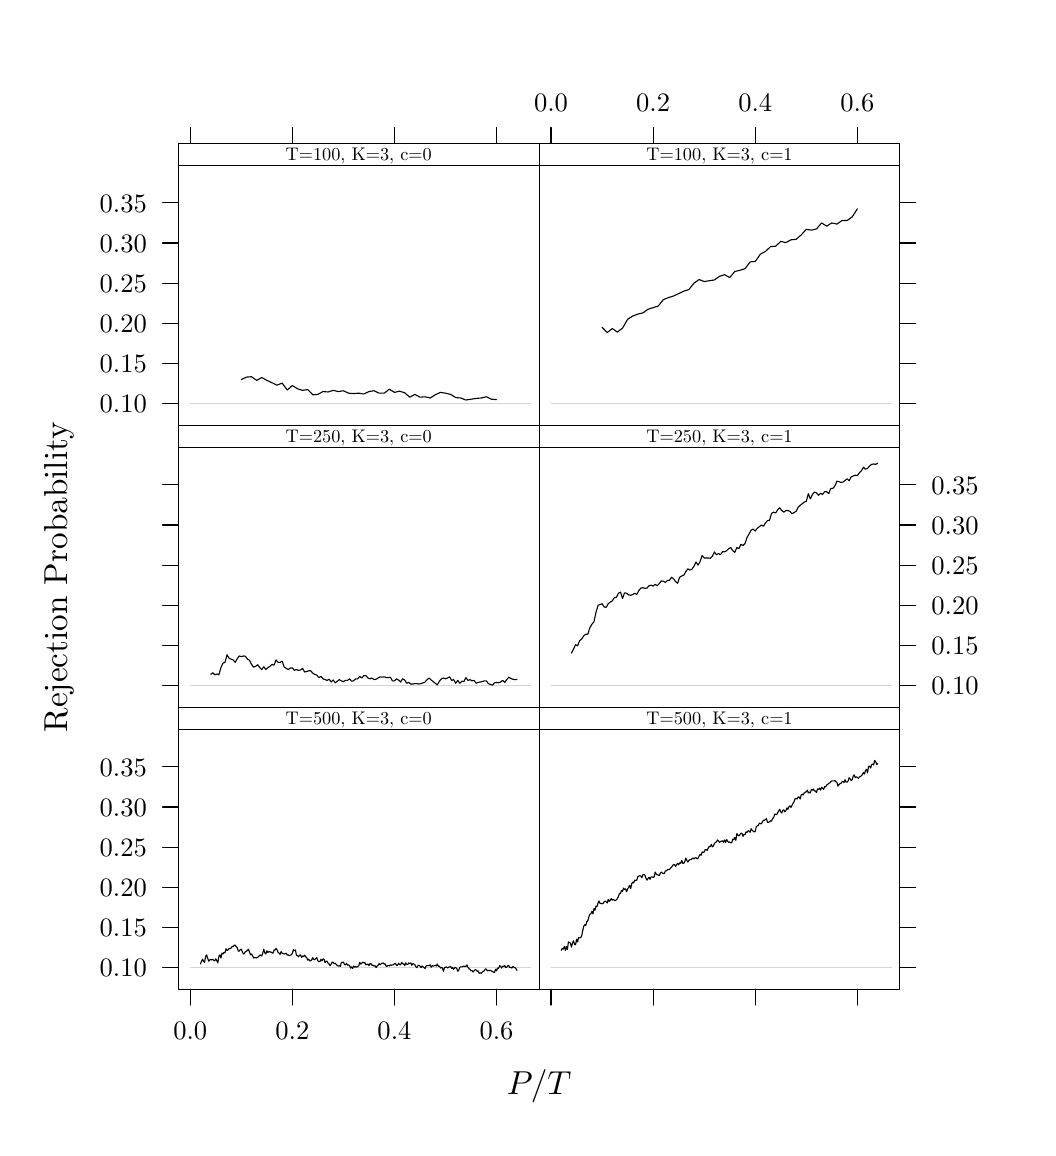
\begin{tikzpicture}[x=1pt,y=1pt]
\definecolor[named]{fillColor}{rgb}{1.00,1.00,1.00}
\path[use as bounding box,fill=fillColor,fill opacity=0.00] (0,0) rectangle (361.35,397.48);
\begin{scope}
\path[clip] (  0.00,  0.00) rectangle (361.35,397.48);

\path[] (  0.00,  0.00) rectangle (361.35,397.48);
\definecolor[named]{drawColor}{rgb}{0.00,0.00,0.00}

\node[text=drawColor,anchor=base,inner sep=0pt, outer sep=0pt, scale=  1.20] at (184.81, 12.04) {$P/T$};
\end{scope}
\begin{scope}
\path[clip] (  0.00,  0.00) rectangle (361.35,397.48);
\definecolor[named]{drawColor}{rgb}{0.00,0.00,0.00}

\node[text=drawColor,rotate= 90.00,anchor=base,inner sep=0pt, outer sep=0pt, scale=  1.20] at ( 14.29,198.90) {Rejection Probability};
\end{scope}
\begin{scope}
\path[clip] (  0.00,  0.00) rectangle (361.35,397.48);
\definecolor[named]{drawColor}{rgb}{0.00,0.00,0.00}

\path[draw=drawColor,line width= 0.4pt,line join=round,line cap=round] ( 54.44, 57.82) -- ( 48.75, 57.82);

\path[draw=drawColor,line width= 0.4pt,line join=round,line cap=round] ( 54.44, 72.33) -- ( 48.75, 72.33);

\path[draw=drawColor,line width= 0.4pt,line join=round,line cap=round] ( 54.44, 86.84) -- ( 48.75, 86.84);

\path[draw=drawColor,line width= 0.4pt,line join=round,line cap=round] ( 54.44,101.35) -- ( 48.75,101.35);

\path[draw=drawColor,line width= 0.4pt,line join=round,line cap=round] ( 54.44,115.86) -- ( 48.75,115.86);

\path[draw=drawColor,line width= 0.4pt,line join=round,line cap=round] ( 54.44,130.37) -- ( 48.75,130.37);

\node[text=drawColor,anchor=base east,inner sep=0pt, outer sep=0pt, scale=  0.96] at ( 43.06, 54.51) {0.10};

\node[text=drawColor,anchor=base east,inner sep=0pt, outer sep=0pt, scale=  0.96] at ( 43.06, 69.02) {0.15};

\node[text=drawColor,anchor=base east,inner sep=0pt, outer sep=0pt, scale=  0.96] at ( 43.06, 83.53) {0.20};

\node[text=drawColor,anchor=base east,inner sep=0pt, outer sep=0pt, scale=  0.96] at ( 43.06, 98.04) {0.25};

\node[text=drawColor,anchor=base east,inner sep=0pt, outer sep=0pt, scale=  0.96] at ( 43.06,112.55) {0.30};

\node[text=drawColor,anchor=base east,inner sep=0pt, outer sep=0pt, scale=  0.96] at ( 43.06,127.06) {0.35};
\end{scope}
\begin{scope}
\path[clip] (  0.00,  0.00) rectangle (361.35,397.48);
\definecolor[named]{drawColor}{rgb}{0.00,0.00,0.00}

\path[draw=drawColor,line width= 0.4pt,line join=round,line cap=round] ( 58.76, 50.02) -- ( 58.76, 44.32);

\path[draw=drawColor,line width= 0.4pt,line join=round,line cap=round] ( 95.65, 50.02) -- ( 95.65, 44.32);

\path[draw=drawColor,line width= 0.4pt,line join=round,line cap=round] (132.54, 50.02) -- (132.54, 44.32);

\path[draw=drawColor,line width= 0.4pt,line join=round,line cap=round] (169.42, 50.02) -- (169.42, 44.32);

\node[text=drawColor,anchor=base,inner sep=0pt, outer sep=0pt, scale=  0.96] at ( 58.76, 32.02) {0.0};

\node[text=drawColor,anchor=base,inner sep=0pt, outer sep=0pt, scale=  0.96] at ( 95.65, 32.02) {0.2};

\node[text=drawColor,anchor=base,inner sep=0pt, outer sep=0pt, scale=  0.96] at (132.54, 32.02) {0.4};

\node[text=drawColor,anchor=base,inner sep=0pt, outer sep=0pt, scale=  0.96] at (169.42, 32.02) {0.6};
\end{scope}
\begin{scope}
\path[clip] ( 54.44, 50.02) rectangle (184.81,143.97);
\definecolor[named]{drawColor}{rgb}{0.83,0.83,0.83}

\path[draw=drawColor,line width= 0.4pt,line join=round,line cap=round] ( 58.76, 57.82) --
	(181.72, 57.82);
\definecolor[named]{drawColor}{rgb}{0.00,0.00,0.00}

\path[draw=drawColor,line width= 0.4pt,line join=round,line cap=round] ( 62.45, 59.12) --
	( 62.82, 60.14) --
	( 63.19, 60.86) --
	( 63.56, 60.14) --
	( 63.92, 59.70) --
	( 64.29, 61.88) --
	( 64.66, 62.46) --
	( 65.03, 61.30) --
	( 65.40, 60.14) --
	( 65.77, 60.57) --
	( 66.14, 60.86) --
	( 66.51, 60.57) --
	( 66.88, 60.86) --
	( 67.24, 60.43) --
	( 67.61, 60.28) --
	( 67.98, 61.01) --
	( 68.35, 60.28) --
	( 68.72, 59.56) --
	( 69.09, 61.88) --
	( 69.46, 62.46) --
	( 69.83, 61.30) --
	( 70.20, 63.04) --
	( 70.56, 62.75) --
	( 70.93, 63.33) --
	( 71.30, 63.18) --
	( 71.67, 64.64) --
	( 72.04, 64.06) --
	( 72.41, 64.20) --
	( 72.78, 64.78) --
	( 73.15, 64.64) --
	( 73.52, 64.93) --
	( 73.88, 65.51) --
	( 74.25, 65.36) --
	( 74.62, 65.94) --
	( 74.99, 65.94) --
	( 75.36, 65.36) --
	( 75.73, 65.07) --
	( 76.10, 63.77) --
	( 76.47, 63.77) --
	( 76.84, 64.35) --
	( 77.20, 64.49) --
	( 77.57, 63.62) --
	( 77.94, 62.75) --
	( 78.31, 62.89) --
	( 78.68, 63.62) --
	( 79.05, 63.77) --
	( 79.42, 64.06) --
	( 79.79, 64.49) --
	( 80.16, 63.48) --
	( 80.52, 62.46) --
	( 80.89, 62.75) --
	( 81.26, 62.17) --
	( 81.63, 61.30) --
	( 82.00, 61.44) --
	( 82.37, 61.44) --
	( 82.74, 61.30) --
	( 83.11, 61.59) --
	( 83.48, 61.88) --
	( 83.84, 62.31) --
	( 84.21, 62.31) --
	( 84.58, 62.02) --
	( 84.95, 63.04) --
	( 85.32, 64.49) --
	( 85.69, 63.18) --
	( 86.06, 62.75) --
	( 86.43, 63.91) --
	( 86.79, 63.33) --
	( 87.16, 63.62) --
	( 87.53, 63.48) --
	( 87.90, 63.48) --
	( 88.27, 63.18) --
	( 88.64, 63.04) --
	( 89.01, 64.20) --
	( 89.38, 64.20) --
	( 89.75, 64.78) --
	( 90.11, 64.20) --
	( 90.48, 63.33) --
	( 90.85, 63.04) --
	( 91.22, 62.60) --
	( 91.59, 63.62) --
	( 91.96, 63.04) --
	( 92.33, 62.89) --
	( 92.70, 62.75) --
	( 93.07, 62.89) --
	( 93.43, 63.04) --
	( 93.80, 62.31) --
	( 94.17, 62.46) --
	( 94.54, 62.17) --
	( 94.91, 62.31) --
	( 95.28, 62.46) --
	( 95.65, 63.04) --
	( 96.02, 64.35) --
	( 96.39, 63.91) --
	( 96.75, 64.20) --
	( 97.12, 62.31) --
	( 97.49, 62.17) --
	( 97.86, 61.73) --
	( 98.23, 62.31) --
	( 98.60, 62.46) --
	( 98.97, 61.44) --
	( 99.34, 62.02) --
	( 99.71, 61.88) --
	(100.07, 62.31) --
	(100.44, 61.73) --
	(100.81, 61.44) --
	(101.18, 60.57) --
	(101.55, 60.86) --
	(101.92, 60.28) --
	(102.29, 60.28) --
	(102.66, 60.72) --
	(103.03, 61.44) --
	(103.39, 60.72) --
	(103.76, 60.72) --
	(104.13, 61.15) --
	(104.50, 61.44) --
	(104.87, 60.28) --
	(105.24, 59.99) --
	(105.61, 59.99) --
	(105.98, 60.86) --
	(106.35, 60.28) --
	(106.71, 61.01) --
	(107.08, 60.86) --
	(107.45, 59.70) --
	(107.82, 60.14) --
	(108.19, 60.14) --
	(108.56, 59.41) --
	(108.93, 59.12) --
	(109.30, 58.54) --
	(109.67, 59.12) --
	(110.03, 59.85) --
	(110.40, 59.70) --
	(110.77, 59.27) --
	(111.14, 59.41) --
	(111.51, 58.98) --
	(111.88, 58.54) --
	(112.25, 58.40) --
	(112.62, 58.54) --
	(112.99, 58.25) --
	(113.35, 59.70) --
	(113.72, 59.70) --
	(114.09, 59.85) --
	(114.46, 58.98) --
	(114.83, 58.83) --
	(115.20, 59.41) --
	(115.57, 58.69) --
	(115.94, 58.83) --
	(116.31, 58.54) --
	(116.67, 57.67) --
	(117.04, 58.11) --
	(117.41, 57.53) --
	(117.78, 58.40) --
	(118.15, 57.96) --
	(118.52, 58.25) --
	(118.89, 57.96) --
	(119.26, 58.25) --
	(119.63, 58.54) --
	(119.99, 59.70) --
	(120.36, 59.12) --
	(120.73, 59.41) --
	(121.10, 59.85) --
	(121.47, 59.56) --
	(121.84, 59.70) --
	(122.21, 58.83) --
	(122.58, 58.98) --
	(122.95, 59.12) --
	(123.31, 58.54) --
	(123.68, 59.27) --
	(124.05, 59.27) --
	(124.42, 58.69) --
	(124.79, 58.69) --
	(125.16, 58.40) --
	(125.53, 58.54) --
	(125.90, 57.82) --
	(126.27, 58.40) --
	(126.63, 58.69) --
	(127.00, 59.27) --
	(127.37, 58.83) --
	(127.74, 59.27) --
	(128.11, 59.41) --
	(128.48, 59.56) --
	(128.85, 59.12) --
	(129.22, 59.12) --
	(129.59, 58.25) --
	(129.95, 58.40) --
	(130.32, 58.69) --
	(130.69, 58.40) --
	(131.06, 58.83) --
	(131.43, 58.69) --
	(131.80, 58.83) --
	(132.17, 58.83) --
	(132.54, 59.27) --
	(132.91, 59.27) --
	(133.27, 58.69) --
	(133.64, 58.69) --
	(134.01, 59.41) --
	(134.38, 58.98) --
	(134.75, 58.83) --
	(135.12, 59.70) --
	(135.49, 59.27) --
	(135.86, 59.12) --
	(136.23, 58.54) --
	(136.59, 59.56) --
	(136.96, 58.98) --
	(137.33, 58.98) --
	(137.70, 59.56) --
	(138.07, 59.27) --
	(138.44, 59.56) --
	(138.81, 58.69) --
	(139.18, 59.27) --
	(139.55, 59.12) --
	(139.91, 58.83) --
	(140.28, 58.11) --
	(140.65, 57.82) --
	(141.02, 58.54) --
	(141.39, 58.69) --
	(141.76, 58.40) --
	(142.13, 57.82) --
	(142.50, 58.40) --
	(142.87, 58.11) --
	(143.23, 57.82) --
	(143.60, 57.53) --
	(143.97, 58.40) --
	(144.34, 58.54) --
	(144.71, 58.54) --
	(145.08, 58.54) --
	(145.45, 58.83) --
	(145.82, 57.96) --
	(146.19, 58.54) --
	(146.55, 58.40) --
	(146.92, 58.54) --
	(147.29, 58.69) --
	(147.66, 58.40) --
	(148.03, 59.12) --
	(148.40, 58.25) --
	(148.77, 58.40) --
	(149.14, 57.67) --
	(149.51, 57.96) --
	(149.87, 57.67) --
	(150.24, 56.51) --
	(150.61, 57.82) --
	(150.98, 57.96) --
	(151.35, 58.11) --
	(151.72, 57.67) --
	(152.09, 57.96) --
	(152.46, 58.11) --
	(152.83, 58.25) --
	(153.19, 57.53) --
	(153.56, 57.82) --
	(153.93, 57.24) --
	(154.30, 57.82) --
	(154.67, 57.82) --
	(155.04, 57.53) --
	(155.41, 56.51) --
	(155.78, 56.95) --
	(156.15, 57.96) --
	(156.51, 58.11) --
	(156.88, 58.11) --
	(157.25, 58.25) --
	(157.62, 58.40) --
	(157.99, 58.25) --
	(158.36, 58.25) --
	(158.73, 58.83) --
	(159.10, 57.96) --
	(159.47, 57.38) --
	(159.83, 57.24) --
	(160.20, 56.66) --
	(160.57, 56.80) --
	(160.94, 56.22) --
	(161.31, 56.66) --
	(161.68, 57.09) --
	(162.05, 56.95) --
	(162.42, 56.51) --
	(162.78, 56.66) --
	(163.15, 55.78) --
	(163.52, 55.93) --
	(163.89, 55.78) --
	(164.26, 56.22) --
	(164.63, 56.51) --
	(165.00, 56.66) --
	(165.37, 57.38) --
	(165.74, 57.24) --
	(166.10, 56.66) --
	(166.47, 56.80) --
	(166.84, 56.80) --
	(167.21, 56.80) --
	(167.58, 56.66) --
	(167.95, 56.37) --
	(168.32, 56.22) --
	(168.69, 56.07) --
	(169.06, 57.24) --
	(169.42, 56.66) --
	(169.79, 57.67) --
	(170.16, 57.53) --
	(170.53, 58.54) --
	(170.90, 58.25) --
	(171.27, 57.67) --
	(171.64, 58.40) --
	(172.01, 58.25) --
	(172.38, 58.54) --
	(172.74, 57.82) --
	(173.11, 57.96) --
	(173.48, 58.54) --
	(173.85, 58.54) --
	(174.22, 57.82) --
	(174.59, 57.96) --
	(174.96, 57.67) --
	(175.33, 58.25) --
	(175.70, 57.96) --
	(176.06, 57.82) --
	(176.43, 57.53) --
	(176.80, 56.80);
\end{scope}
\begin{scope}
\path[clip] (  0.00,  0.00) rectangle (361.35,397.48);
\definecolor[named]{drawColor}{rgb}{0.00,0.00,0.00}

\path[draw=drawColor,line width= 0.4pt,line join=round,line cap=round] ( 54.44, 50.02) rectangle (184.81,143.97);
\end{scope}
\begin{scope}
\path[clip] ( 54.44,143.97) rectangle (184.81,151.92);

\path[] ( 54.44,143.97) rectangle (184.81,151.92);
\definecolor[named]{drawColor}{rgb}{0.00,0.00,0.00}

\node[text=drawColor,anchor=base west,inner sep=0pt, outer sep=0pt, scale=  0.66] at ( 93.23,145.67) {T=500, K=3, c=0};
\end{scope}
\begin{scope}
\path[clip] (  0.00,  0.00) rectangle (361.35,397.48);
\definecolor[named]{drawColor}{rgb}{0.00,0.00,0.00}

\path[draw=drawColor,line width= 0.4pt,line join=round,line cap=round] ( 54.44,143.97) rectangle (184.81,151.92);
\end{scope}
\begin{scope}
\path[clip] (  0.00,  0.00) rectangle (361.35,397.48);
\definecolor[named]{drawColor}{rgb}{0.00,0.00,0.00}

\path[draw=drawColor,line width= 0.4pt,line join=round,line cap=round] (189.12, 50.02) -- (189.12, 44.32);

\path[draw=drawColor,line width= 0.4pt,line join=round,line cap=round] (226.01, 50.02) -- (226.01, 44.32);

\path[draw=drawColor,line width= 0.4pt,line join=round,line cap=round] (262.90, 50.02) -- (262.90, 44.32);

\path[draw=drawColor,line width= 0.4pt,line join=round,line cap=round] (299.79, 50.02) -- (299.79, 44.32);

\path[draw=drawColor,line width= 0.4pt,line join=round,line cap=round] (315.17, 57.82) -- (320.86, 57.82);

\path[draw=drawColor,line width= 0.4pt,line join=round,line cap=round] (315.17, 72.33) -- (320.86, 72.33);

\path[draw=drawColor,line width= 0.4pt,line join=round,line cap=round] (315.17, 86.84) -- (320.86, 86.84);

\path[draw=drawColor,line width= 0.4pt,line join=round,line cap=round] (315.17,101.35) -- (320.86,101.35);

\path[draw=drawColor,line width= 0.4pt,line join=round,line cap=round] (315.17,115.86) -- (320.86,115.86);

\path[draw=drawColor,line width= 0.4pt,line join=round,line cap=round] (315.17,130.37) -- (320.86,130.37);
\end{scope}
\begin{scope}
\path[clip] (184.81, 50.02) rectangle (315.17,143.97);
\definecolor[named]{drawColor}{rgb}{0.83,0.83,0.83}

\path[draw=drawColor,line width= 0.4pt,line join=round,line cap=round] (189.12, 57.82) --
	(312.08, 57.82);
\definecolor[named]{drawColor}{rgb}{0.00,0.00,0.00}

\path[draw=drawColor,line width= 0.4pt,line join=round,line cap=round] (192.81, 64.06) --
	(193.18, 64.78) --
	(193.55, 64.49) --
	(193.92, 65.51) --
	(194.29, 64.06) --
	(194.66, 65.51) --
	(195.03, 64.35) --
	(195.39, 67.10) --
	(195.76, 66.96) --
	(196.13, 66.67) --
	(196.50, 65.22) --
	(196.87, 66.67) --
	(197.24, 67.54) --
	(197.61, 66.23) --
	(197.98, 66.09) --
	(198.35, 68.12) --
	(198.71, 67.10) --
	(199.08, 68.70) --
	(199.45, 68.55) --
	(199.82, 68.70) --
	(200.19, 69.28) --
	(200.56, 71.17) --
	(200.93, 72.76) --
	(201.30, 73.34) --
	(201.67, 73.05) --
	(202.03, 74.36) --
	(202.40, 74.79) --
	(202.77, 76.10) --
	(203.14, 77.11) --
	(203.51, 77.26) --
	(203.88, 78.13) --
	(204.25, 77.26) --
	(204.62, 79.15) --
	(204.99, 78.57) --
	(205.35, 80.02) --
	(205.72, 79.87) --
	(206.09, 81.18) --
	(206.46, 81.90) --
	(206.83, 81.03) --
	(207.20, 81.03) --
	(207.57, 80.89) --
	(207.94, 81.03) --
	(208.31, 81.61) --
	(208.67, 81.90) --
	(209.04, 81.61) --
	(209.41, 81.18) --
	(209.78, 82.48) --
	(210.15, 81.76) --
	(210.52, 82.19) --
	(210.89, 82.77) --
	(211.26, 82.19) --
	(211.63, 82.48) --
	(211.99, 82.19) --
	(212.36, 82.05) --
	(212.73, 82.34) --
	(213.10, 82.77) --
	(213.47, 83.50) --
	(213.84, 84.66) --
	(214.21, 84.66) --
	(214.58, 85.68) --
	(214.95, 85.39) --
	(215.31, 86.55) --
	(215.68, 86.11) --
	(216.05, 86.26) --
	(216.42, 85.24) --
	(216.79, 86.26) --
	(217.16, 86.84) --
	(217.53, 87.56) --
	(217.90, 86.40) --
	(218.27, 88.14) --
	(218.63, 88.72) --
	(219.00, 88.43) --
	(219.37, 89.45) --
	(219.74, 89.30) --
	(220.11, 89.45) --
	(220.48, 90.75) --
	(220.85, 90.90) --
	(221.22, 91.04) --
	(221.58, 90.90) --
	(221.95, 90.32) --
	(222.32, 91.48) --
	(222.69, 91.48) --
	(223.06, 91.19) --
	(223.43, 90.03) --
	(223.80, 89.45) --
	(224.17, 90.03) --
	(224.54, 90.46) --
	(224.90, 89.74) --
	(225.27, 90.61) --
	(225.64, 90.61) --
	(226.01, 90.46) --
	(226.38, 90.61) --
	(226.75, 92.35) --
	(227.12, 91.62) --
	(227.49, 91.33) --
	(227.86, 91.33) --
	(228.22, 91.04) --
	(228.59, 91.92) --
	(228.96, 92.35) --
	(229.33, 92.06) --
	(229.70, 91.77) --
	(230.07, 91.92) --
	(230.44, 92.79) --
	(230.81, 92.79) --
	(231.18, 93.22) --
	(231.54, 93.22) --
	(231.91, 93.22) --
	(232.28, 93.80) --
	(232.65, 94.09) --
	(233.02, 94.67) --
	(233.39, 95.11) --
	(233.76, 94.96) --
	(234.13, 94.38) --
	(234.50, 95.11) --
	(234.86, 95.54) --
	(235.23, 94.96) --
	(235.60, 95.69) --
	(235.97, 95.54) --
	(236.34, 96.56) --
	(236.71, 95.54) --
	(237.08, 95.54) --
	(237.45, 96.12) --
	(237.82, 97.43) --
	(238.18, 96.56) --
	(238.55, 95.98) --
	(238.92, 96.56) --
	(239.29, 96.85) --
	(239.66, 96.85) --
	(240.03, 97.14) --
	(240.40, 97.43) --
	(240.77, 97.14) --
	(241.14, 97.43) --
	(241.50, 97.57) --
	(241.87, 97.14) --
	(242.24, 97.28) --
	(242.61, 98.15) --
	(242.98, 98.74) --
	(243.35, 98.44) --
	(243.72, 99.61) --
	(244.09, 99.46) --
	(244.46, 99.61) --
	(244.82,100.48) --
	(245.19,100.48) --
	(245.56,100.19) --
	(245.93,101.06) --
	(246.30,101.64) --
	(246.67,101.49) --
	(247.04,102.36) --
	(247.41,101.49) --
	(247.78,101.78) --
	(248.14,102.65) --
	(248.51,103.09) --
	(248.88,103.23) --
	(249.25,103.96) --
	(249.62,103.67) --
	(249.99,103.09) --
	(250.36,103.38) --
	(250.73,103.52) --
	(251.10,103.67) --
	(251.46,103.09) --
	(251.83,103.96) --
	(252.20,103.09) --
	(252.57,104.10) --
	(252.94,103.52) --
	(253.31,103.09) --
	(253.68,103.23) --
	(254.05,102.94) --
	(254.42,102.94) --
	(254.78,104.25) --
	(255.15,104.10) --
	(255.52,104.83) --
	(255.89,103.81) --
	(256.26,106.28) --
	(256.63,105.70) --
	(257.00,105.41) --
	(257.37,105.85) --
	(257.74,106.43) --
	(258.10,106.43) --
	(258.47,105.26) --
	(258.84,105.99) --
	(259.21,105.85) --
	(259.58,106.86) --
	(259.95,106.72) --
	(260.32,107.30) --
	(260.69,107.15) --
	(261.06,106.72) --
	(261.42,108.02) --
	(261.79,107.44) --
	(262.16,107.15) --
	(262.53,106.86) --
	(262.90,107.01) --
	(263.27,108.75) --
	(263.64,109.04) --
	(264.01,109.18) --
	(264.38,110.05) --
	(264.74,109.91) --
	(265.11,109.76) --
	(265.48,110.49) --
	(265.85,111.07) --
	(266.22,111.07) --
	(266.59,111.36) --
	(266.96,111.65) --
	(267.33,110.34) --
	(267.70,110.34) --
	(268.06,110.49) --
	(268.43,110.92) --
	(268.80,110.78) --
	(269.17,111.79) --
	(269.54,111.94) --
	(269.91,113.25) --
	(270.28,113.25) --
	(270.65,113.10) --
	(271.02,113.83) --
	(271.38,114.41) --
	(271.75,114.99) --
	(272.12,114.12) --
	(272.49,113.68) --
	(272.86,114.70) --
	(273.23,114.84) --
	(273.60,114.12) --
	(273.97,114.55) --
	(274.34,115.57) --
	(274.70,114.99) --
	(275.07,116.00) --
	(275.44,116.29) --
	(275.81,115.71) --
	(276.18,116.44) --
	(276.55,117.16) --
	(276.92,117.74) --
	(277.29,118.90) --
	(277.66,118.90) --
	(278.02,118.76) --
	(278.39,119.48) --
	(278.76,119.48) --
	(279.13,118.76) --
	(279.50,120.21) --
	(279.87,120.50) --
	(280.24,120.21) --
	(280.61,120.94) --
	(280.98,121.23) --
	(281.34,121.37) --
	(281.71,121.95) --
	(282.08,120.94) --
	(282.45,121.23) --
	(282.82,120.94) --
	(283.19,122.24) --
	(283.56,121.95) --
	(283.93,122.39) --
	(284.30,121.66) --
	(284.66,121.66) --
	(285.03,121.08) --
	(285.40,122.39) --
	(285.77,122.24) --
	(286.14,122.68) --
	(286.51,121.95) --
	(286.88,122.97) --
	(287.25,122.68) --
	(287.62,122.24) --
	(287.98,123.26) --
	(288.35,123.11) --
	(288.72,123.84) --
	(289.09,123.98) --
	(289.46,124.42) --
	(289.83,124.56) --
	(290.20,125.00) --
	(290.57,125.29) --
	(290.94,125.29) --
	(291.30,125.29) --
	(291.67,125.43) --
	(292.04,125.00) --
	(292.41,124.85) --
	(292.78,123.40) --
	(293.15,123.98) --
	(293.52,124.27) --
	(293.89,124.42) --
	(294.26,125.00) --
	(294.62,125.14) --
	(294.99,124.71) --
	(295.36,125.72) --
	(295.73,124.85) --
	(296.10,124.85) --
	(296.47,125.29) --
	(296.84,126.45) --
	(297.21,126.01) --
	(297.58,125.43) --
	(297.94,125.72) --
	(298.31,127.03) --
	(298.68,127.47) --
	(299.05,126.45) --
	(299.42,126.74) --
	(299.79,126.59) --
	(300.16,126.16) --
	(300.53,126.74) --
	(300.89,126.88) --
	(301.26,127.18) --
	(301.63,127.61) --
	(302.00,128.34) --
	(302.37,127.76) --
	(302.74,129.06) --
	(303.11,129.50) --
	(303.48,128.19) --
	(303.85,130.51) --
	(304.21,130.66) --
	(304.58,129.93) --
	(304.95,131.09) --
	(305.32,131.38) --
	(305.69,131.09) --
	(306.06,132.69) --
	(306.43,132.25) --
	(306.80,131.24) --
	(307.17,131.53);
\end{scope}
\begin{scope}
\path[clip] (  0.00,  0.00) rectangle (361.35,397.48);
\definecolor[named]{drawColor}{rgb}{0.00,0.00,0.00}

\path[draw=drawColor,line width= 0.4pt,line join=round,line cap=round] (184.81, 50.02) rectangle (315.17,143.97);
\end{scope}
\begin{scope}
\path[clip] (184.81,143.97) rectangle (315.17,151.92);

\path[] (184.81,143.97) rectangle (315.17,151.92);
\definecolor[named]{drawColor}{rgb}{0.00,0.00,0.00}

\node[text=drawColor,anchor=base west,inner sep=0pt, outer sep=0pt, scale=  0.66] at (223.60,145.67) {T=500, K=3, c=1};
\end{scope}
\begin{scope}
\path[clip] (  0.00,  0.00) rectangle (361.35,397.48);
\definecolor[named]{drawColor}{rgb}{0.00,0.00,0.00}

\path[draw=drawColor,line width= 0.4pt,line join=round,line cap=round] (184.81,143.97) rectangle (315.17,151.92);
\end{scope}
\begin{scope}
\path[clip] (  0.00,  0.00) rectangle (361.35,397.48);
\definecolor[named]{drawColor}{rgb}{0.00,0.00,0.00}

\path[draw=drawColor,line width= 0.4pt,line join=round,line cap=round] ( 54.44,159.72) -- ( 48.75,159.72);

\path[draw=drawColor,line width= 0.4pt,line join=round,line cap=round] ( 54.44,174.23) -- ( 48.75,174.23);

\path[draw=drawColor,line width= 0.4pt,line join=round,line cap=round] ( 54.44,188.74) -- ( 48.75,188.74);

\path[draw=drawColor,line width= 0.4pt,line join=round,line cap=round] ( 54.44,203.25) -- ( 48.75,203.25);

\path[draw=drawColor,line width= 0.4pt,line join=round,line cap=round] ( 54.44,217.76) -- ( 48.75,217.76);

\path[draw=drawColor,line width= 0.4pt,line join=round,line cap=round] ( 54.44,232.27) -- ( 48.75,232.27);
\end{scope}
\begin{scope}
\path[clip] ( 54.44,151.92) rectangle (184.81,245.88);
\definecolor[named]{drawColor}{rgb}{0.83,0.83,0.83}

\path[draw=drawColor,line width= 0.4pt,line join=round,line cap=round] ( 58.76,159.72) --
	(181.72,159.72);
\definecolor[named]{drawColor}{rgb}{0.00,0.00,0.00}

\path[draw=drawColor,line width= 0.4pt,line join=round,line cap=round] ( 66.14,163.79) --
	( 66.88,164.37) --
	( 67.61,163.64) --
	( 68.35,163.93) --
	( 69.09,163.64) --
	( 69.83,166.25) --
	( 70.56,167.85) --
	( 71.30,168.14) --
	( 72.04,170.90) --
	( 72.78,169.59) --
	( 73.52,169.30) --
	( 74.25,169.01) --
	( 74.99,168.14) --
	( 75.73,169.44) --
	( 76.47,170.46) --
	( 77.20,170.17) --
	( 77.94,170.46) --
	( 78.68,170.31) --
	( 79.42,169.30) --
	( 80.16,168.86) --
	( 80.89,167.41) --
	( 81.63,166.40) --
	( 82.37,166.69) --
	( 83.11,167.27) --
	( 83.84,166.25) --
	( 84.58,165.53) --
	( 85.32,166.54) --
	( 86.06,165.53) --
	( 86.79,166.25) --
	( 87.53,166.69) --
	( 88.27,167.41) --
	( 89.01,167.12) --
	( 89.75,169.01) --
	( 90.48,168.14) --
	( 91.22,168.14) --
	( 91.96,168.57) --
	( 92.70,166.40) --
	( 93.43,165.96) --
	( 94.17,165.53) --
	( 94.91,166.11) --
	( 95.65,166.11) --
	( 96.39,165.24) --
	( 97.12,165.53) --
	( 97.86,165.24) --
	( 98.60,165.38) --
	( 99.34,165.96) --
	(100.07,164.66) --
	(100.81,164.80) --
	(101.55,165.09) --
	(102.29,165.09) --
	(103.03,164.22) --
	(103.76,163.79) --
	(104.50,163.50) --
	(105.24,162.62) --
	(105.98,163.06) --
	(106.71,162.19) --
	(107.45,161.90) --
	(108.19,161.61) --
	(108.93,162.04) --
	(109.67,161.03) --
	(110.40,161.75) --
	(111.14,160.74) --
	(111.88,161.32) --
	(112.62,161.90) --
	(113.35,161.46) --
	(114.09,161.17) --
	(114.83,161.61) --
	(115.57,161.61) --
	(116.31,162.19) --
	(117.04,161.32) --
	(117.78,161.46) --
	(118.52,162.19) --
	(119.26,162.19) --
	(119.99,163.06) --
	(120.73,162.48) --
	(121.47,163.35) --
	(122.21,163.35) --
	(122.95,162.48) --
	(123.68,162.19) --
	(124.42,162.48) --
	(125.16,161.90) --
	(125.90,162.04) --
	(126.63,162.48) --
	(127.37,162.91) --
	(128.11,162.77) --
	(128.85,162.91) --
	(129.59,162.62) --
	(130.32,162.62) --
	(131.06,162.77) --
	(131.80,161.46) --
	(132.54,161.46) --
	(133.27,162.19) --
	(134.01,161.75) --
	(134.75,161.03) --
	(135.49,162.19) --
	(136.23,161.75) --
	(136.96,160.59) --
	(137.70,160.88) --
	(138.44,160.30) --
	(139.18,160.30) --
	(139.91,160.45) --
	(140.65,160.45) --
	(141.39,160.30) --
	(142.13,160.45) --
	(142.87,160.74) --
	(143.60,161.03) --
	(144.34,161.90) --
	(145.08,162.48) --
	(145.82,161.75) --
	(146.55,161.17) --
	(147.29,160.59) --
	(148.03,160.01) --
	(148.77,161.32) --
	(149.51,162.19) --
	(150.24,162.48) --
	(150.98,162.19) --
	(151.72,162.48) --
	(152.46,162.91) --
	(153.19,161.61) --
	(153.93,161.90) --
	(154.67,160.59) --
	(155.41,161.61) --
	(156.15,160.59) --
	(156.88,161.32) --
	(157.62,161.17) --
	(158.36,162.62) --
	(159.10,161.61) --
	(159.83,161.90) --
	(160.57,161.46) --
	(161.31,161.61) --
	(162.05,160.59) --
	(162.78,160.88) --
	(163.52,161.03) --
	(164.26,161.17) --
	(165.00,161.46) --
	(165.74,161.46) --
	(166.47,160.45) --
	(167.21,160.16) --
	(167.95,159.87) --
	(168.69,160.74) --
	(169.42,160.88) --
	(170.16,160.74) --
	(170.90,161.03) --
	(171.64,161.61) --
	(172.38,160.88) --
	(173.11,161.90) --
	(173.85,162.77) --
	(174.59,162.33) --
	(175.33,162.04) --
	(176.06,161.90) --
	(176.80,161.90);
\end{scope}
\begin{scope}
\path[clip] (  0.00,  0.00) rectangle (361.35,397.48);
\definecolor[named]{drawColor}{rgb}{0.00,0.00,0.00}

\path[draw=drawColor,line width= 0.4pt,line join=round,line cap=round] ( 54.44,151.92) rectangle (184.81,245.88);
\end{scope}
\begin{scope}
\path[clip] ( 54.44,245.88) rectangle (184.81,253.83);

\path[] ( 54.44,245.88) rectangle (184.81,253.83);
\definecolor[named]{drawColor}{rgb}{0.00,0.00,0.00}

\node[text=drawColor,anchor=base west,inner sep=0pt, outer sep=0pt, scale=  0.66] at ( 93.23,247.58) {T=250, K=3, c=0};
\end{scope}
\begin{scope}
\path[clip] (  0.00,  0.00) rectangle (361.35,397.48);
\definecolor[named]{drawColor}{rgb}{0.00,0.00,0.00}

\path[draw=drawColor,line width= 0.4pt,line join=round,line cap=round] ( 54.44,245.88) rectangle (184.81,253.83);
\end{scope}
\begin{scope}
\path[clip] (  0.00,  0.00) rectangle (361.35,397.48);
\definecolor[named]{drawColor}{rgb}{0.00,0.00,0.00}

\path[draw=drawColor,line width= 0.4pt,line join=round,line cap=round] (315.17,159.72) -- (320.86,159.72);

\path[draw=drawColor,line width= 0.4pt,line join=round,line cap=round] (315.17,174.23) -- (320.86,174.23);

\path[draw=drawColor,line width= 0.4pt,line join=round,line cap=round] (315.17,188.74) -- (320.86,188.74);

\path[draw=drawColor,line width= 0.4pt,line join=round,line cap=round] (315.17,203.25) -- (320.86,203.25);

\path[draw=drawColor,line width= 0.4pt,line join=round,line cap=round] (315.17,217.76) -- (320.86,217.76);

\path[draw=drawColor,line width= 0.4pt,line join=round,line cap=round] (315.17,232.27) -- (320.86,232.27);

\node[text=drawColor,anchor=base west,inner sep=0pt, outer sep=0pt, scale=  0.96] at (326.55,156.42) {0.10};

\node[text=drawColor,anchor=base west,inner sep=0pt, outer sep=0pt, scale=  0.96] at (326.55,170.93) {0.15};

\node[text=drawColor,anchor=base west,inner sep=0pt, outer sep=0pt, scale=  0.96] at (326.55,185.44) {0.20};

\node[text=drawColor,anchor=base west,inner sep=0pt, outer sep=0pt, scale=  0.96] at (326.55,199.95) {0.25};

\node[text=drawColor,anchor=base west,inner sep=0pt, outer sep=0pt, scale=  0.96] at (326.55,214.46) {0.30};

\node[text=drawColor,anchor=base west,inner sep=0pt, outer sep=0pt, scale=  0.96] at (326.55,228.97) {0.35};
\end{scope}
\begin{scope}
\path[clip] (184.81,151.92) rectangle (315.17,245.88);
\definecolor[named]{drawColor}{rgb}{0.83,0.83,0.83}

\path[draw=drawColor,line width= 0.4pt,line join=round,line cap=round] (189.12,159.72) --
	(312.08,159.72);
\definecolor[named]{drawColor}{rgb}{0.00,0.00,0.00}

\path[draw=drawColor,line width= 0.4pt,line join=round,line cap=round] (196.50,171.48) --
	(197.24,172.93) --
	(197.98,174.52) --
	(198.71,174.09) --
	(199.45,175.97) --
	(200.19,176.55) --
	(200.93,177.72) --
	(201.67,178.30) --
	(202.40,178.30) --
	(203.14,180.62) --
	(203.88,181.92) --
	(204.62,182.79) --
	(205.35,186.13) --
	(206.09,188.74) --
	(206.83,189.03) --
	(207.57,189.32) --
	(208.31,188.16) --
	(209.04,188.02) --
	(209.78,189.32) --
	(210.52,189.90) --
	(211.26,190.34) --
	(211.99,191.50) --
	(212.73,191.64) --
	(213.47,193.10) --
	(214.21,193.53) --
	(214.95,191.21) --
	(215.68,193.24) --
	(216.42,193.10) --
	(217.16,192.52) --
	(217.90,192.37) --
	(218.63,192.66) --
	(219.37,193.10) --
	(220.11,192.66) --
	(220.85,194.11) --
	(221.58,194.98) --
	(222.32,195.13) --
	(223.06,194.84) --
	(223.80,194.98) --
	(224.54,195.85) --
	(225.27,196.00) --
	(226.01,195.71) --
	(226.75,196.29) --
	(227.49,195.85) --
	(228.22,196.58) --
	(228.96,197.59) --
	(229.70,197.45) --
	(230.44,197.01) --
	(231.18,197.74) --
	(231.91,197.74) --
	(232.65,198.90) --
	(233.39,198.32) --
	(234.13,197.30) --
	(234.86,196.72) --
	(235.60,198.90) --
	(236.34,199.34) --
	(237.08,199.63) --
	(237.82,200.93) --
	(238.55,201.95) --
	(239.29,201.51) --
	(240.03,201.80) --
	(240.77,202.82) --
	(241.50,204.41) --
	(242.24,203.25) --
	(242.98,204.56) --
	(243.72,206.74) --
	(244.46,205.86) --
	(245.19,205.86) --
	(245.93,205.86) --
	(246.67,205.72) --
	(247.41,206.45) --
	(248.14,208.04) --
	(248.88,207.03) --
	(249.62,207.46) --
	(250.36,207.03) --
	(251.10,208.19) --
	(251.83,208.04) --
	(252.57,208.48) --
	(253.31,209.20) --
	(254.05,209.64) --
	(254.78,208.48) --
	(255.52,207.90) --
	(256.26,209.64) --
	(257.00,209.20) --
	(257.74,210.80) --
	(258.47,210.36) --
	(259.21,211.09) --
	(259.95,213.27) --
	(260.69,214.57) --
	(261.42,215.88) --
	(262.16,216.31) --
	(262.90,215.59) --
	(263.64,216.60) --
	(264.38,217.18) --
	(265.11,217.76) --
	(265.85,217.33) --
	(266.59,218.49) --
	(267.33,219.36) --
	(268.06,219.50) --
	(268.80,221.97) --
	(269.54,222.41) --
	(270.28,222.12) --
	(271.02,223.28) --
	(271.75,224.00) --
	(272.49,222.99) --
	(273.23,222.41) --
	(273.97,222.99) --
	(274.70,222.99) --
	(275.44,222.70) --
	(276.18,221.83) --
	(276.92,222.26) --
	(277.66,222.70) --
	(278.39,224.15) --
	(279.13,224.87) --
	(279.87,225.45) --
	(280.61,226.03) --
	(281.34,226.32) --
	(282.08,229.08) --
	(282.82,227.19) --
	(283.56,228.79) --
	(284.30,229.66) --
	(285.03,229.37) --
	(285.77,228.50) --
	(286.51,229.23) --
	(287.25,228.79) --
	(287.98,229.81) --
	(288.72,229.81) --
	(289.46,229.08) --
	(290.20,230.97) --
	(290.94,230.97) --
	(291.67,231.84) --
	(292.41,233.58) --
	(293.15,233.43) --
	(293.89,233.14) --
	(294.62,233.29) --
	(295.36,233.87) --
	(296.10,234.45) --
	(296.84,233.72) --
	(297.58,235.18) --
	(298.31,235.47) --
	(299.05,235.76) --
	(299.79,235.61) --
	(300.53,236.63) --
	(301.26,237.35) --
	(302.00,238.66) --
	(302.74,237.93) --
	(303.48,238.22) --
	(304.21,239.09) --
	(304.95,239.67) --
	(305.69,239.82) --
	(306.43,239.67) --
	(307.17,240.11);
\end{scope}
\begin{scope}
\path[clip] (  0.00,  0.00) rectangle (361.35,397.48);
\definecolor[named]{drawColor}{rgb}{0.00,0.00,0.00}

\path[draw=drawColor,line width= 0.4pt,line join=round,line cap=round] (184.81,151.92) rectangle (315.17,245.88);
\end{scope}
\begin{scope}
\path[clip] (184.81,245.88) rectangle (315.17,253.83);

\path[] (184.81,245.88) rectangle (315.17,253.83);
\definecolor[named]{drawColor}{rgb}{0.00,0.00,0.00}

\node[text=drawColor,anchor=base west,inner sep=0pt, outer sep=0pt, scale=  0.66] at (223.60,247.58) {T=250, K=3, c=1};
\end{scope}
\begin{scope}
\path[clip] (  0.00,  0.00) rectangle (361.35,397.48);
\definecolor[named]{drawColor}{rgb}{0.00,0.00,0.00}

\path[draw=drawColor,line width= 0.4pt,line join=round,line cap=round] (184.81,245.88) rectangle (315.17,253.83);
\end{scope}
\begin{scope}
\path[clip] (  0.00,  0.00) rectangle (361.35,397.48);
\definecolor[named]{drawColor}{rgb}{0.00,0.00,0.00}

\path[draw=drawColor,line width= 0.4pt,line join=round,line cap=round] ( 58.76,355.73) -- ( 58.76,361.42);

\path[draw=drawColor,line width= 0.4pt,line join=round,line cap=round] ( 95.65,355.73) -- ( 95.65,361.42);

\path[draw=drawColor,line width= 0.4pt,line join=round,line cap=round] (132.54,355.73) -- (132.54,361.42);

\path[draw=drawColor,line width= 0.4pt,line join=round,line cap=round] (169.42,355.73) -- (169.42,361.42);
\end{scope}
\begin{scope}
\path[clip] (  0.00,  0.00) rectangle (361.35,397.48);
\definecolor[named]{drawColor}{rgb}{0.00,0.00,0.00}

\path[draw=drawColor,line width= 0.4pt,line join=round,line cap=round] ( 54.44,261.63) -- ( 48.75,261.63);

\path[draw=drawColor,line width= 0.4pt,line join=round,line cap=round] ( 54.44,276.14) -- ( 48.75,276.14);

\path[draw=drawColor,line width= 0.4pt,line join=round,line cap=round] ( 54.44,290.65) -- ( 48.75,290.65);

\path[draw=drawColor,line width= 0.4pt,line join=round,line cap=round] ( 54.44,305.16) -- ( 48.75,305.16);

\path[draw=drawColor,line width= 0.4pt,line join=round,line cap=round] ( 54.44,319.67) -- ( 48.75,319.67);

\path[draw=drawColor,line width= 0.4pt,line join=round,line cap=round] ( 54.44,334.18) -- ( 48.75,334.18);

\node[text=drawColor,anchor=base east,inner sep=0pt, outer sep=0pt, scale=  0.96] at ( 43.06,258.32) {0.10};

\node[text=drawColor,anchor=base east,inner sep=0pt, outer sep=0pt, scale=  0.96] at ( 43.06,272.83) {0.15};

\node[text=drawColor,anchor=base east,inner sep=0pt, outer sep=0pt, scale=  0.96] at ( 43.06,287.34) {0.20};

\node[text=drawColor,anchor=base east,inner sep=0pt, outer sep=0pt, scale=  0.96] at ( 43.06,301.85) {0.25};

\node[text=drawColor,anchor=base east,inner sep=0pt, outer sep=0pt, scale=  0.96] at ( 43.06,316.36) {0.30};

\node[text=drawColor,anchor=base east,inner sep=0pt, outer sep=0pt, scale=  0.96] at ( 43.06,330.87) {0.35};
\end{scope}
\begin{scope}
\path[clip] ( 54.44,253.83) rectangle (184.81,347.78);
\definecolor[named]{drawColor}{rgb}{0.83,0.83,0.83}

\path[draw=drawColor,line width= 0.4pt,line join=round,line cap=round] ( 58.76,261.63) --
	(181.72,261.63);
\definecolor[named]{drawColor}{rgb}{0.00,0.00,0.00}

\path[draw=drawColor,line width= 0.4pt,line join=round,line cap=round] ( 77.20,270.33) --
	( 79.05,271.21) --
	( 80.89,271.35) --
	( 82.74,270.04) --
	( 84.58,271.06) --
	( 86.43,270.04) --
	( 88.27,269.17) --
	( 90.11,268.30) --
	( 91.96,269.03) --
	( 93.80,266.56) --
	( 95.65,268.16) --
	( 97.49,267.00) --
	( 99.34,266.42) --
	(101.18,266.71) --
	(103.03,264.82) --
	(104.87,264.97) --
	(106.71,265.98) --
	(108.56,265.84) --
	(110.40,266.42) --
	(112.25,265.98) --
	(114.09,266.27) --
	(115.94,265.40) --
	(117.78,265.26) --
	(119.63,265.40) --
	(121.47,265.11) --
	(123.31,265.98) --
	(125.16,266.27) --
	(127.00,265.40) --
	(128.85,265.40) --
	(130.69,266.85) --
	(132.54,265.69) --
	(134.38,266.13) --
	(136.23,265.55) --
	(138.07,263.95) --
	(139.91,264.97) --
	(141.76,263.95) --
	(143.60,264.10) --
	(145.45,263.66) --
	(147.29,264.82) --
	(149.14,265.69) --
	(150.98,265.40) --
	(152.83,264.97) --
	(154.67,263.81) --
	(156.51,263.66) --
	(158.36,262.93) --
	(160.20,263.22) --
	(162.05,263.51) --
	(163.89,263.66) --
	(165.74,264.10) --
	(167.58,263.22) --
	(169.42,263.08);
\end{scope}
\begin{scope}
\path[clip] (  0.00,  0.00) rectangle (361.35,397.48);
\definecolor[named]{drawColor}{rgb}{0.00,0.00,0.00}

\path[draw=drawColor,line width= 0.4pt,line join=round,line cap=round] ( 54.44,253.83) rectangle (184.81,347.78);
\end{scope}
\begin{scope}
\path[clip] ( 54.44,347.78) rectangle (184.81,355.73);

\path[] ( 54.44,347.78) rectangle (184.81,355.73);
\definecolor[named]{drawColor}{rgb}{0.00,0.00,0.00}

\node[text=drawColor,anchor=base west,inner sep=0pt, outer sep=0pt, scale=  0.66] at ( 93.23,349.49) {T=100, K=3, c=0};
\end{scope}
\begin{scope}
\path[clip] (  0.00,  0.00) rectangle (361.35,397.48);
\definecolor[named]{drawColor}{rgb}{0.00,0.00,0.00}

\path[draw=drawColor,line width= 0.4pt,line join=round,line cap=round] ( 54.44,347.78) rectangle (184.81,355.73);
\end{scope}
\begin{scope}
\path[clip] (  0.00,  0.00) rectangle (361.35,397.48);
\definecolor[named]{drawColor}{rgb}{0.00,0.00,0.00}

\path[draw=drawColor,line width= 0.4pt,line join=round,line cap=round] (189.12,355.73) -- (189.12,361.42);

\path[draw=drawColor,line width= 0.4pt,line join=round,line cap=round] (226.01,355.73) -- (226.01,361.42);

\path[draw=drawColor,line width= 0.4pt,line join=round,line cap=round] (262.90,355.73) -- (262.90,361.42);

\path[draw=drawColor,line width= 0.4pt,line join=round,line cap=round] (299.79,355.73) -- (299.79,361.42);

\node[text=drawColor,anchor=base,inner sep=0pt, outer sep=0pt, scale=  0.96] at (189.12,367.12) {0.0};

\node[text=drawColor,anchor=base,inner sep=0pt, outer sep=0pt, scale=  0.96] at (226.01,367.12) {0.2};

\node[text=drawColor,anchor=base,inner sep=0pt, outer sep=0pt, scale=  0.96] at (262.90,367.12) {0.4};

\node[text=drawColor,anchor=base,inner sep=0pt, outer sep=0pt, scale=  0.96] at (299.79,367.12) {0.6};
\end{scope}
\begin{scope}
\path[clip] (  0.00,  0.00) rectangle (361.35,397.48);
\definecolor[named]{drawColor}{rgb}{0.00,0.00,0.00}

\path[draw=drawColor,line width= 0.4pt,line join=round,line cap=round] (315.17,261.63) -- (320.86,261.63);

\path[draw=drawColor,line width= 0.4pt,line join=round,line cap=round] (315.17,276.14) -- (320.86,276.14);

\path[draw=drawColor,line width= 0.4pt,line join=round,line cap=round] (315.17,290.65) -- (320.86,290.65);

\path[draw=drawColor,line width= 0.4pt,line join=round,line cap=round] (315.17,305.16) -- (320.86,305.16);

\path[draw=drawColor,line width= 0.4pt,line join=round,line cap=round] (315.17,319.67) -- (320.86,319.67);

\path[draw=drawColor,line width= 0.4pt,line join=round,line cap=round] (315.17,334.18) -- (320.86,334.18);
\end{scope}
\begin{scope}
\path[clip] (184.81,253.83) rectangle (315.17,347.78);
\definecolor[named]{drawColor}{rgb}{0.83,0.83,0.83}

\path[draw=drawColor,line width= 0.4pt,line join=round,line cap=round] (189.12,261.63) --
	(312.08,261.63);
\definecolor[named]{drawColor}{rgb}{0.00,0.00,0.00}

\path[draw=drawColor,line width= 0.4pt,line join=round,line cap=round] (207.57,289.20) --
	(209.41,287.31) --
	(211.26,288.76) --
	(213.10,287.46) --
	(214.95,288.91) --
	(216.79,292.10) --
	(218.63,293.26) --
	(220.48,293.99) --
	(222.32,294.42) --
	(224.17,295.73) --
	(226.01,296.31) --
	(227.86,296.89) --
	(229.70,299.21) --
	(231.54,299.94) --
	(233.39,300.52) --
	(235.23,301.39) --
	(237.08,302.26) --
	(238.92,302.84) --
	(240.77,305.16) --
	(242.61,306.47) --
	(244.46,305.74) --
	(246.30,306.03) --
	(248.14,306.32) --
	(249.99,307.63) --
	(251.83,308.21) --
	(253.68,307.19) --
	(255.52,309.37) --
	(257.37,309.80) --
	(259.21,310.38) --
	(261.06,312.85) --
	(262.90,312.99) --
	(264.74,315.61) --
	(266.59,316.62) --
	(268.43,318.36) --
	(270.28,318.51) --
	(272.12,320.25) --
	(273.97,319.81) --
	(275.81,320.83) --
	(277.66,320.98) --
	(279.50,322.57) --
	(281.34,324.60) --
	(283.19,324.31) --
	(285.03,324.75) --
	(286.88,326.92) --
	(288.72,325.76) --
	(290.57,326.92) --
	(292.41,326.49) --
	(294.26,327.80) --
	(296.10,327.80) --
	(297.94,329.10) --
	(299.79,332.00);
\end{scope}
\begin{scope}
\path[clip] (  0.00,  0.00) rectangle (361.35,397.48);
\definecolor[named]{drawColor}{rgb}{0.00,0.00,0.00}

\path[draw=drawColor,line width= 0.4pt,line join=round,line cap=round] (184.81,253.83) rectangle (315.17,347.78);
\end{scope}
\begin{scope}
\path[clip] (184.81,347.78) rectangle (315.17,355.73);

\path[] (184.81,347.78) rectangle (315.17,355.73);
\definecolor[named]{drawColor}{rgb}{0.00,0.00,0.00}

\node[text=drawColor,anchor=base west,inner sep=0pt, outer sep=0pt, scale=  0.66] at (223.60,349.49) {T=100, K=3, c=1};
\end{scope}
\begin{scope}
\path[clip] (  0.00,  0.00) rectangle (361.35,397.48);
\definecolor[named]{drawColor}{rgb}{0.00,0.00,0.00}

\path[draw=drawColor,line width= 0.4pt,line join=round,line cap=round] (184.81,347.78) rectangle (315.17,355.73);
\end{scope}
\end{tikzpicture}

  \caption{Simulated rejection probabilities for McCracken's (2007)
    recursive \oost\ test under the null hypothesis that the benchmark
    model is more accurate, $\E_T \oosB \leq 0$. Nominal size is 10\%
    and is marked with a solid horizontal line. Values greater than
    10\% indicate that the test rejects the benchmark model too
    often.}
  \label{fig:mccracken}
\end{figure}

\begin{figure}\centering
  {\large Power of recursive DMW \oost\ test in simulations}
  % Created by tikzDevice version 0.6.2-92-0ad2792 on 2014-03-27 14:58:15
% !TEX encoding = UTF-8 Unicode
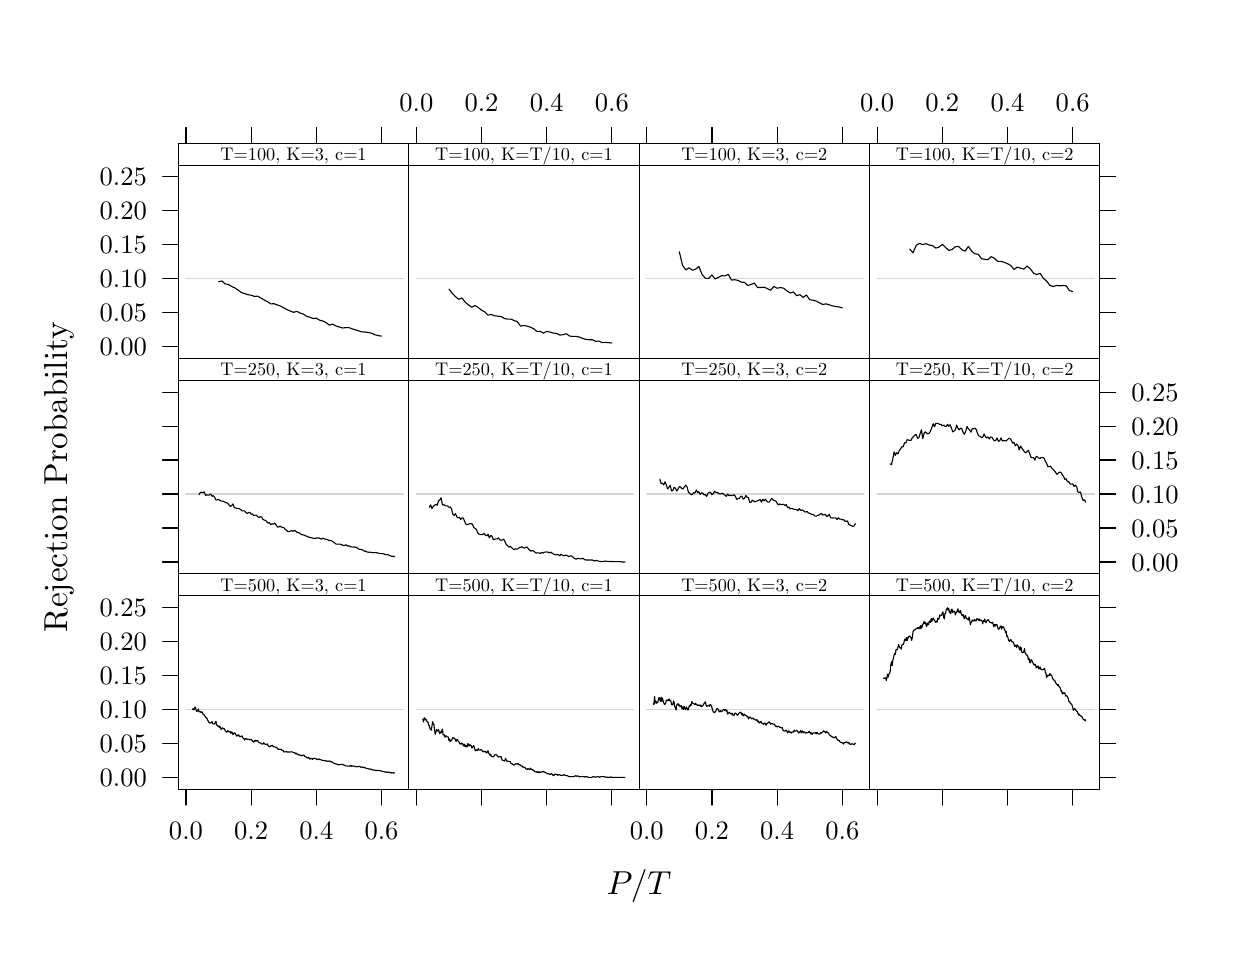
\begin{tikzpicture}[x=1pt,y=1pt]
\definecolor[named]{fillColor}{rgb}{1.00,1.00,1.00}
\path[use as bounding box,fill=fillColor,fill opacity=0.00] (0,0) rectangle (433.62,325.21);
\begin{scope}
\path[clip] (  0.00,  0.00) rectangle (433.62,325.21);

\path[] (  0.00,  0.00) rectangle (433.62,325.21);
\definecolor[named]{drawColor}{rgb}{0.00,0.00,0.00}

\node[text=drawColor,anchor=base,inner sep=0pt, outer sep=0pt, scale=  1.20] at (220.94, 12.05) {$P/T$};
\end{scope}
\begin{scope}
\path[clip] (  0.00,  0.00) rectangle (433.62,325.21);
\definecolor[named]{drawColor}{rgb}{0.00,0.00,0.00}

\node[text=drawColor,rotate= 90.00,anchor=base,inner sep=0pt, outer sep=0pt, scale=  1.20] at ( 14.29,162.76) {Rejection Probability};
\end{scope}
\begin{scope}
\path[clip] (  0.00,  0.00) rectangle (433.62,325.21);
\definecolor[named]{drawColor}{rgb}{0.00,0.00,0.00}

\path[draw=drawColor,line width= 0.4pt,line join=round,line cap=round] ( 54.44, 54.31) -- ( 48.75, 54.31);

\path[draw=drawColor,line width= 0.4pt,line join=round,line cap=round] ( 54.44, 66.59) -- ( 48.75, 66.59);

\path[draw=drawColor,line width= 0.4pt,line join=round,line cap=round] ( 54.44, 78.87) -- ( 48.75, 78.87);

\path[draw=drawColor,line width= 0.4pt,line join=round,line cap=round] ( 54.44, 91.15) -- ( 48.75, 91.15);

\path[draw=drawColor,line width= 0.4pt,line join=round,line cap=round] ( 54.44,103.43) -- ( 48.75,103.43);

\path[draw=drawColor,line width= 0.4pt,line join=round,line cap=round] ( 54.44,115.71) -- ( 48.75,115.71);

\node[text=drawColor,anchor=base east,inner sep=0pt, outer sep=0pt, scale=  0.96] at ( 43.06, 51.00) {0.00};

\node[text=drawColor,anchor=base east,inner sep=0pt, outer sep=0pt, scale=  0.96] at ( 43.06, 63.28) {0.05};

\node[text=drawColor,anchor=base east,inner sep=0pt, outer sep=0pt, scale=  0.96] at ( 43.06, 75.56) {0.10};

\node[text=drawColor,anchor=base east,inner sep=0pt, outer sep=0pt, scale=  0.96] at ( 43.06, 87.85) {0.15};

\node[text=drawColor,anchor=base east,inner sep=0pt, outer sep=0pt, scale=  0.96] at ( 43.06,100.13) {0.20};

\node[text=drawColor,anchor=base east,inner sep=0pt, outer sep=0pt, scale=  0.96] at ( 43.06,112.41) {0.25};
\end{scope}
\begin{scope}
\path[clip] (  0.00,  0.00) rectangle (433.62,325.21);
\definecolor[named]{drawColor}{rgb}{0.00,0.00,0.00}

\path[draw=drawColor,line width= 0.4pt,line join=round,line cap=round] ( 57.20, 50.02) -- ( 57.20, 44.32);

\path[draw=drawColor,line width= 0.4pt,line join=round,line cap=round] ( 80.76, 50.02) -- ( 80.76, 44.32);

\path[draw=drawColor,line width= 0.4pt,line join=round,line cap=round] (104.31, 50.02) -- (104.31, 44.32);

\path[draw=drawColor,line width= 0.4pt,line join=round,line cap=round] (127.87, 50.02) -- (127.87, 44.32);

\node[text=drawColor,anchor=base,inner sep=0pt, outer sep=0pt, scale=  0.96] at ( 57.20, 32.02) {0.0};

\node[text=drawColor,anchor=base,inner sep=0pt, outer sep=0pt, scale=  0.96] at ( 80.76, 32.02) {0.2};

\node[text=drawColor,anchor=base,inner sep=0pt, outer sep=0pt, scale=  0.96] at (104.31, 32.02) {0.4};

\node[text=drawColor,anchor=base,inner sep=0pt, outer sep=0pt, scale=  0.96] at (127.87, 32.02) {0.6};
\end{scope}
\begin{scope}
\path[clip] ( 54.44, 50.02) rectangle (137.69,119.88);
\definecolor[named]{drawColor}{rgb}{0.83,0.83,0.83}

\path[draw=drawColor,line width= 0.4pt,line join=round,line cap=round] ( 57.20, 78.87) --
	(135.72, 78.87);
\definecolor[named]{drawColor}{rgb}{0.00,0.00,0.00}

\path[draw=drawColor,line width= 0.4pt,line join=round,line cap=round] ( 59.56, 78.85) --
	( 59.79, 79.14) --
	( 60.03, 78.68) --
	( 60.26, 79.14) --
	( 60.50, 79.72) --
	( 60.73, 79.32) --
	( 60.97, 78.15) --
	( 61.20, 78.21) --
	( 61.44, 78.39) --
	( 61.68, 79.03) --
	( 61.91, 77.98) --
	( 62.15, 78.04) --
	( 62.38, 78.04) --
	( 62.62, 77.75) --
	( 62.85, 77.98) --
	( 63.09, 77.92) --
	( 63.32, 77.22) --
	( 63.56, 76.99) --
	( 63.80, 76.87) --
	( 64.03, 76.47) --
	( 64.27, 76.12) --
	( 64.50, 75.77) --
	( 64.74, 75.77) --
	( 64.97, 75.07) --
	( 65.21, 74.72) --
	( 65.44, 74.20) --
	( 65.68, 74.14) --
	( 65.92, 73.91) --
	( 66.15, 74.02) --
	( 66.39, 74.14) --
	( 66.62, 74.49) --
	( 66.86, 73.73) --
	( 67.09, 73.68) --
	( 67.33, 73.56) --
	( 67.56, 73.56) --
	( 67.80, 74.31) --
	( 68.04, 74.55) --
	( 68.27, 73.27) --
	( 68.51, 73.09) --
	( 68.74, 72.74) --
	( 68.98, 72.86) --
	( 69.21, 72.40) --
	( 69.45, 72.86) --
	( 69.69, 72.05) --
	( 69.92, 71.58) --
	( 70.16, 72.05) --
	( 70.39, 72.22) --
	( 70.63, 71.87) --
	( 70.86, 71.93) --
	( 71.10, 71.81) --
	( 71.33, 71.29) --
	( 71.57, 70.94) --
	( 71.81, 70.65) --
	( 72.04, 70.65) --
	( 72.28, 71.23) --
	( 72.51, 71.00) --
	( 72.75, 70.71) --
	( 72.98, 70.82) --
	( 73.22, 70.88) --
	( 73.45, 70.24) --
	( 73.69, 70.71) --
	( 73.93, 70.48) --
	( 74.16, 69.78) --
	( 74.40, 70.01) --
	( 74.63, 70.42) --
	( 74.87, 70.36) --
	( 75.10, 70.07) --
	( 75.34, 69.49) --
	( 75.57, 69.20) --
	( 75.81, 69.55) --
	( 76.05, 69.37) --
	( 76.28, 69.66) --
	( 76.52, 69.08) --
	( 76.75, 69.08) --
	( 76.99, 68.96) --
	( 77.22, 69.20) --
	( 77.46, 69.31) --
	( 77.69, 68.73) --
	( 77.93, 68.32) --
	( 78.17, 68.27) --
	( 78.40, 67.80) --
	( 78.64, 68.27) --
	( 78.87, 68.44) --
	( 79.11, 68.21) --
	( 79.34, 68.03) --
	( 79.58, 68.09) --
	( 79.81, 68.15) --
	( 80.05, 67.97) --
	( 80.29, 67.86) --
	( 80.52, 67.92) --
	( 80.76, 68.09) --
	( 80.99, 67.80) --
	( 81.23, 67.28) --
	( 81.46, 67.33) --
	( 81.70, 67.04) --
	( 81.93, 67.63) --
	( 82.17, 67.39) --
	( 82.41, 67.68) --
	( 82.64, 67.39) --
	( 82.88, 67.63) --
	( 83.11, 67.63) --
	( 83.35, 67.10) --
	( 83.58, 66.87) --
	( 83.82, 66.75) --
	( 84.05, 66.75) --
	( 84.29, 66.64) --
	( 84.53, 66.40) --
	( 84.76, 66.35) --
	( 85.00, 66.29) --
	( 85.23, 66.81) --
	( 85.47, 66.58) --
	( 85.70, 66.29) --
	( 85.94, 66.29) --
	( 86.17, 66.17) --
	( 86.41, 66.17) --
	( 86.65, 66.40) --
	( 86.88, 65.65) --
	( 87.12, 65.65) --
	( 87.35, 65.30) --
	( 87.59, 65.47) --
	( 87.82, 65.65) --
	( 88.06, 65.76) --
	( 88.29, 65.65) --
	( 88.53, 65.88) --
	( 88.77, 65.36) --
	( 89.00, 65.36) --
	( 89.24, 65.30) --
	( 89.47, 65.30) --
	( 89.71, 65.18) --
	( 89.94, 65.12) --
	( 90.18, 64.83) --
	( 90.41, 64.60) --
	( 90.65, 64.37) --
	( 90.89, 64.54) --
	( 91.12, 64.37) --
	( 91.36, 64.43) --
	( 91.59, 64.48) --
	( 91.83, 64.14) --
	( 92.06, 64.08) --
	( 92.30, 64.08) --
	( 92.53, 63.50) --
	( 92.77, 63.55) --
	( 93.01, 63.50) --
	( 93.24, 63.55) --
	( 93.48, 63.67) --
	( 93.71, 63.50) --
	( 93.95, 63.38) --
	( 94.18, 63.55) --
	( 94.42, 63.44) --
	( 94.66, 63.44) --
	( 94.89, 63.50) --
	( 95.13, 63.50) --
	( 95.36, 63.55) --
	( 95.60, 63.50) --
	( 95.83, 63.38) --
	( 96.07, 63.26) --
	( 96.30, 63.26) --
	( 96.54, 63.15) --
	( 96.78, 62.80) --
	( 97.01, 63.09) --
	( 97.25, 62.86) --
	( 97.48, 62.57) --
	( 97.72, 62.68) --
	( 97.95, 62.39) --
	( 98.19, 62.39) --
	( 98.42, 62.45) --
	( 98.66, 62.22) --
	( 98.90, 62.10) --
	( 99.13, 62.10) --
	( 99.37, 62.33) --
	( 99.60, 62.39) --
	( 99.84, 62.33) --
	(100.07, 61.93) --
	(100.31, 61.81) --
	(100.54, 61.69) --
	(100.78, 61.52) --
	(101.02, 61.29) --
	(101.25, 61.34) --
	(101.49, 61.58) --
	(101.72, 61.17) --
	(101.96, 60.88) --
	(102.19, 61.05) --
	(102.43, 61.23) --
	(102.66, 61.05) --
	(102.90, 60.82) --
	(103.14, 61.11) --
	(103.37, 61.05) --
	(103.61, 61.29) --
	(103.84, 61.05) --
	(104.08, 61.05) --
	(104.31, 60.94) --
	(104.55, 60.70) --
	(104.78, 60.82) --
	(105.02, 60.88) --
	(105.26, 60.99) --
	(105.49, 60.70) --
	(105.73, 60.70) --
	(105.96, 60.76) --
	(106.20, 60.53) --
	(106.43, 60.47) --
	(106.67, 60.47) --
	(106.90, 60.41) --
	(107.14, 60.30) --
	(107.38, 60.41) --
	(107.61, 60.30) --
	(107.85, 60.12) --
	(108.08, 60.24) --
	(108.32, 60.18) --
	(108.55, 60.12) --
	(108.79, 60.12) --
	(109.02, 60.24) --
	(109.26, 60.18) --
	(109.50, 60.06) --
	(109.73, 59.83) --
	(109.97, 59.89) --
	(110.20, 59.77) --
	(110.44, 59.54) --
	(110.67, 59.37) --
	(110.91, 59.25) --
	(111.14, 59.25) --
	(111.38, 59.13) --
	(111.62, 59.13) --
	(111.85, 59.02) --
	(112.09, 58.96) --
	(112.32, 58.84) --
	(112.56, 58.96) --
	(112.79, 58.96) --
	(113.03, 58.96) --
	(113.26, 58.96) --
	(113.50, 59.02) --
	(113.74, 58.96) --
	(113.97, 58.90) --
	(114.21, 58.84) --
	(114.44, 58.61) --
	(114.68, 58.67) --
	(114.91, 58.49) --
	(115.15, 58.44) --
	(115.38, 58.44) --
	(115.62, 58.38) --
	(115.86, 58.38) --
	(116.09, 58.38) --
	(116.33, 58.32) --
	(116.56, 58.67) --
	(116.80, 58.61) --
	(117.03, 58.26) --
	(117.27, 58.49) --
	(117.51, 58.44) --
	(117.74, 58.38) --
	(117.98, 58.38) --
	(118.21, 58.32) --
	(118.45, 58.20) --
	(118.68, 58.09) --
	(118.92, 58.09) --
	(119.15, 58.14) --
	(119.39, 58.20) --
	(119.63, 58.26) --
	(119.86, 58.26) --
	(120.10, 58.14) --
	(120.33, 57.97) --
	(120.57, 58.03) --
	(120.80, 58.09) --
	(121.04, 57.85) --
	(121.27, 57.97) --
	(121.51, 57.85) --
	(121.75, 57.80) --
	(121.98, 57.80) --
	(122.22, 57.56) --
	(122.45, 57.56) --
	(122.69, 57.45) --
	(122.92, 57.50) --
	(123.16, 57.33) --
	(123.39, 57.39) --
	(123.63, 57.33) --
	(123.87, 57.21) --
	(124.10, 57.27) --
	(124.34, 57.21) --
	(124.57, 56.98) --
	(124.81, 56.92) --
	(125.04, 56.98) --
	(125.28, 56.98) --
	(125.51, 56.81) --
	(125.75, 56.75) --
	(125.99, 56.86) --
	(126.22, 56.75) --
	(126.46, 56.81) --
	(126.69, 56.75) --
	(126.93, 56.75) --
	(127.16, 56.81) --
	(127.40, 56.75) --
	(127.63, 56.63) --
	(127.87, 56.52) --
	(128.11, 56.46) --
	(128.34, 56.46) --
	(128.58, 56.40) --
	(128.81, 56.34) --
	(129.05, 56.40) --
	(129.28, 56.17) --
	(129.52, 56.23) --
	(129.75, 56.11) --
	(129.99, 56.28) --
	(130.23, 56.17) --
	(130.46, 56.11) --
	(130.70, 56.17) --
	(130.93, 56.05) --
	(131.17, 55.93) --
	(131.40, 56.05) --
	(131.64, 55.88) --
	(131.87, 55.93) --
	(132.11, 55.99) --
	(132.35, 55.82) --
	(132.58, 55.93);
\end{scope}
\begin{scope}
\path[clip] (  0.00,  0.00) rectangle (433.62,325.21);
\definecolor[named]{drawColor}{rgb}{0.00,0.00,0.00}

\path[draw=drawColor,line width= 0.4pt,line join=round,line cap=round] ( 54.44, 50.02) rectangle (137.69,119.88);
\end{scope}
\begin{scope}
\path[clip] ( 54.44,119.88) rectangle (137.69,127.83);

\path[] ( 54.44,119.88) rectangle (137.69,127.83);
\definecolor[named]{drawColor}{rgb}{0.00,0.00,0.00}

\node[text=drawColor,anchor=base west,inner sep=0pt, outer sep=0pt, scale=  0.66] at ( 69.67,121.58) {T=500, K=3, c=1};
\end{scope}
\begin{scope}
\path[clip] (  0.00,  0.00) rectangle (433.62,325.21);
\definecolor[named]{drawColor}{rgb}{0.00,0.00,0.00}

\path[draw=drawColor,line width= 0.4pt,line join=round,line cap=round] ( 54.44,119.88) rectangle (137.69,127.83);
\end{scope}
\begin{scope}
\path[clip] (  0.00,  0.00) rectangle (433.62,325.21);
\definecolor[named]{drawColor}{rgb}{0.00,0.00,0.00}

\path[draw=drawColor,line width= 0.4pt,line join=round,line cap=round] (140.45, 50.02) -- (140.45, 44.32);

\path[draw=drawColor,line width= 0.4pt,line join=round,line cap=round] (164.01, 50.02) -- (164.01, 44.32);

\path[draw=drawColor,line width= 0.4pt,line join=round,line cap=round] (187.56, 50.02) -- (187.56, 44.32);

\path[draw=drawColor,line width= 0.4pt,line join=round,line cap=round] (211.12, 50.02) -- (211.12, 44.32);
\end{scope}
\begin{scope}
\path[clip] (137.69, 50.02) rectangle (220.94,119.88);
\definecolor[named]{drawColor}{rgb}{0.83,0.83,0.83}

\path[draw=drawColor,line width= 0.4pt,line join=round,line cap=round] (140.45, 78.87) --
	(218.97, 78.87);
\definecolor[named]{drawColor}{rgb}{0.00,0.00,0.00}

\path[draw=drawColor,line width= 0.4pt,line join=round,line cap=round] (142.80, 75.31) --
	(143.04, 74.32) --
	(143.28, 75.80) --
	(143.51, 75.80) --
	(143.75, 75.06) --
	(143.98, 75.18) --
	(144.22, 74.69) --
	(144.45, 74.32) --
	(144.69, 74.20) --
	(144.92, 73.10) --
	(145.16, 72.97) --
	(145.40, 71.75) --
	(145.63, 71.62) --
	(145.87, 71.38) --
	(146.10, 72.97) --
	(146.34, 74.45) --
	(146.57, 73.71) --
	(146.81, 73.34) --
	(147.05, 71.13) --
	(147.28, 69.90) --
	(147.52, 70.64) --
	(147.75, 71.62) --
	(147.99, 71.13) --
	(148.22, 71.13) --
	(148.46, 71.62) --
	(148.69, 70.64) --
	(148.93, 70.15) --
	(149.17, 70.76) --
	(149.40, 70.39) --
	(149.64, 71.13) --
	(149.87, 71.75) --
	(150.11, 69.66) --
	(150.34, 69.78) --
	(150.58, 69.66) --
	(150.81, 68.80) --
	(151.05, 69.29) --
	(151.29, 69.29) --
	(151.52, 68.92) --
	(151.76, 68.92) --
	(151.99, 68.92) --
	(152.23, 67.57) --
	(152.46, 68.18) --
	(152.70, 67.20) --
	(152.93, 67.69) --
	(153.17, 67.69) --
	(153.41, 68.18) --
	(153.64, 68.68) --
	(153.88, 68.55) --
	(154.11, 68.43) --
	(154.35, 68.43) --
	(154.58, 67.69) --
	(154.82, 67.32) --
	(155.05, 67.94) --
	(155.29, 68.06) --
	(155.53, 67.45) --
	(155.76, 67.20) --
	(156.00, 66.83) --
	(156.23, 66.34) --
	(156.47, 66.34) --
	(156.70, 66.71) --
	(156.94, 66.34) --
	(157.17, 66.59) --
	(157.41, 65.85) --
	(157.65, 65.60) --
	(157.88, 66.34) --
	(158.12, 65.48) --
	(158.35, 65.36) --
	(158.59, 65.85) --
	(158.82, 65.36) --
	(159.06, 66.59) --
	(159.29, 65.97) --
	(159.53, 65.60) --
	(159.77, 66.22) --
	(160.00, 65.85) --
	(160.24, 65.85) --
	(160.47, 64.99) --
	(160.71, 64.99) --
	(160.94, 65.60) --
	(161.18, 65.85) --
	(161.41, 65.11) --
	(161.65, 64.25) --
	(161.89, 63.89) --
	(162.12, 64.25) --
	(162.36, 64.01) --
	(162.59, 64.13) --
	(162.83, 64.75) --
	(163.06, 64.13) --
	(163.30, 64.13) --
	(163.53, 64.13) --
	(163.77, 64.38) --
	(164.01, 64.25) --
	(164.24, 64.01) --
	(164.48, 63.64) --
	(164.71, 63.64) --
	(164.95, 63.52) --
	(165.18, 63.76) --
	(165.42, 63.76) --
	(165.65, 63.27) --
	(165.89, 63.15) --
	(166.13, 63.76) --
	(166.36, 63.89) --
	(166.60, 63.03) --
	(166.83, 62.66) --
	(167.07, 62.29) --
	(167.30, 62.66) --
	(167.54, 61.92) --
	(167.77, 61.92) --
	(168.01, 61.67) --
	(168.25, 61.80) --
	(168.48, 61.92) --
	(168.72, 62.41) --
	(168.95, 62.41) --
	(169.19, 62.53) --
	(169.42, 62.41) --
	(169.66, 62.17) --
	(169.90, 61.80) --
	(170.13, 61.67) --
	(170.37, 61.80) --
	(170.60, 61.67) --
	(170.84, 61.80) --
	(171.07, 61.80) --
	(171.31, 60.94) --
	(171.54, 60.45) --
	(171.78, 60.32) --
	(172.02, 60.45) --
	(172.25, 60.20) --
	(172.49, 60.57) --
	(172.72, 61.18) --
	(172.96, 60.57) --
	(173.19, 60.08) --
	(173.43, 60.20) --
	(173.66, 60.08) --
	(173.90, 60.08) --
	(174.14, 60.08) --
	(174.37, 60.08) --
	(174.61, 59.34) --
	(174.84, 59.22) --
	(175.08, 59.22) --
	(175.31, 58.97) --
	(175.55, 58.73) --
	(175.78, 58.85) --
	(176.02, 58.85) --
	(176.26, 59.22) --
	(176.49, 59.22) --
	(176.73, 59.10) --
	(176.96, 59.10) --
	(177.20, 59.34) --
	(177.43, 58.85) --
	(177.67, 58.85) --
	(177.90, 58.85) --
	(178.14, 58.73) --
	(178.38, 58.36) --
	(178.61, 58.48) --
	(178.85, 57.99) --
	(179.08, 58.11) --
	(179.32, 57.99) --
	(179.55, 57.87) --
	(179.79, 57.74) --
	(180.02, 57.38) --
	(180.26, 57.25) --
	(180.50, 57.13) --
	(180.73, 57.50) --
	(180.97, 57.38) --
	(181.20, 57.13) --
	(181.44, 57.25) --
	(181.67, 57.62) --
	(181.91, 57.25) --
	(182.14, 57.25) --
	(182.38, 57.13) --
	(182.62, 56.76) --
	(182.85, 56.88) --
	(183.09, 56.52) --
	(183.32, 56.27) --
	(183.56, 56.27) --
	(183.79, 56.39) --
	(184.03, 56.15) --
	(184.26, 56.03) --
	(184.50, 56.39) --
	(184.74, 56.03) --
	(184.97, 56.27) --
	(185.21, 56.15) --
	(185.44, 56.27) --
	(185.68, 56.15) --
	(185.91, 56.39) --
	(186.15, 56.27) --
	(186.38, 56.52) --
	(186.62, 56.27) --
	(186.86, 56.15) --
	(187.09, 56.15) --
	(187.33, 55.90) --
	(187.56, 55.78) --
	(187.80, 55.53) --
	(188.03, 55.78) --
	(188.27, 55.66) --
	(188.50, 55.41) --
	(188.74, 55.29) --
	(188.98, 55.41) --
	(189.21, 55.66) --
	(189.45, 55.53) --
	(189.68, 55.29) --
	(189.92, 54.92) --
	(190.15, 55.04) --
	(190.39, 55.29) --
	(190.62, 55.41) --
	(190.86, 55.53) --
	(191.10, 55.29) --
	(191.33, 55.29) --
	(191.57, 55.04) --
	(191.80, 55.17) --
	(192.04, 55.29) --
	(192.27, 55.29) --
	(192.51, 55.04) --
	(192.74, 55.04) --
	(192.98, 55.04) --
	(193.22, 55.04) --
	(193.45, 55.17) --
	(193.69, 55.17) --
	(193.92, 55.29) --
	(194.16, 55.04) --
	(194.39, 54.92) --
	(194.63, 54.92) --
	(194.87, 54.92) --
	(195.10, 54.92) --
	(195.34, 54.67) --
	(195.57, 54.55) --
	(195.81, 54.55) --
	(196.04, 54.55) --
	(196.28, 54.55) --
	(196.51, 54.55) --
	(196.75, 54.55) --
	(196.99, 54.55) --
	(197.22, 54.55) --
	(197.46, 54.67) --
	(197.69, 54.80) --
	(197.93, 54.80) --
	(198.16, 54.92) --
	(198.40, 54.67) --
	(198.63, 54.80) --
	(198.87, 54.80) --
	(199.11, 54.67) --
	(199.34, 54.43) --
	(199.58, 54.55) --
	(199.81, 54.55) --
	(200.05, 54.55) --
	(200.28, 54.67) --
	(200.52, 54.55) --
	(200.75, 54.55) --
	(200.99, 54.55) --
	(201.23, 54.43) --
	(201.46, 54.55) --
	(201.70, 54.43) --
	(201.93, 54.55) --
	(202.17, 54.55) --
	(202.40, 54.43) --
	(202.64, 54.31) --
	(202.87, 54.31) --
	(203.11, 54.31) --
	(203.35, 54.31) --
	(203.58, 54.31) --
	(203.82, 54.31) --
	(204.05, 54.43) --
	(204.29, 54.55) --
	(204.52, 54.55) --
	(204.76, 54.43) --
	(204.99, 54.43) --
	(205.23, 54.43) --
	(205.47, 54.43) --
	(205.70, 54.43) --
	(205.94, 54.55) --
	(206.17, 54.55) --
	(206.41, 54.55) --
	(206.64, 54.31) --
	(206.88, 54.43) --
	(207.11, 54.55) --
	(207.35, 54.55) --
	(207.59, 54.55) --
	(207.82, 54.55) --
	(208.06, 54.55) --
	(208.29, 54.55) --
	(208.53, 54.43) --
	(208.76, 54.43) --
	(209.00, 54.43) --
	(209.23, 54.31) --
	(209.47, 54.43) --
	(209.71, 54.31) --
	(209.94, 54.31) --
	(210.18, 54.31) --
	(210.41, 54.43) --
	(210.65, 54.43) --
	(210.88, 54.31) --
	(211.12, 54.43) --
	(211.35, 54.31) --
	(211.59, 54.31) --
	(211.83, 54.31) --
	(212.06, 54.31) --
	(212.30, 54.31) --
	(212.53, 54.31) --
	(212.77, 54.31) --
	(213.00, 54.31) --
	(213.24, 54.31) --
	(213.47, 54.31) --
	(213.71, 54.31) --
	(213.95, 54.31) --
	(214.18, 54.31) --
	(214.42, 54.31) --
	(214.65, 54.31) --
	(214.89, 54.31) --
	(215.12, 54.31) --
	(215.36, 54.31) --
	(215.59, 54.31) --
	(215.83, 54.31);
\end{scope}
\begin{scope}
\path[clip] (  0.00,  0.00) rectangle (433.62,325.21);
\definecolor[named]{drawColor}{rgb}{0.00,0.00,0.00}

\path[draw=drawColor,line width= 0.4pt,line join=round,line cap=round] (137.69, 50.02) rectangle (220.94,119.88);
\end{scope}
\begin{scope}
\path[clip] (137.69,119.88) rectangle (220.94,127.83);

\path[] (137.69,119.88) rectangle (220.94,127.83);
\definecolor[named]{drawColor}{rgb}{0.00,0.00,0.00}

\node[text=drawColor,anchor=base west,inner sep=0pt, outer sep=0pt, scale=  0.66] at (147.24,121.58) {T=500, K=T/10, c=1};
\end{scope}
\begin{scope}
\path[clip] (  0.00,  0.00) rectangle (433.62,325.21);
\definecolor[named]{drawColor}{rgb}{0.00,0.00,0.00}

\path[draw=drawColor,line width= 0.4pt,line join=round,line cap=round] (137.69,119.88) rectangle (220.94,127.83);
\end{scope}
\begin{scope}
\path[clip] (  0.00,  0.00) rectangle (433.62,325.21);
\definecolor[named]{drawColor}{rgb}{0.00,0.00,0.00}

\path[draw=drawColor,line width= 0.4pt,line join=round,line cap=round] (223.70, 50.02) -- (223.70, 44.32);

\path[draw=drawColor,line width= 0.4pt,line join=round,line cap=round] (247.26, 50.02) -- (247.26, 44.32);

\path[draw=drawColor,line width= 0.4pt,line join=round,line cap=round] (270.81, 50.02) -- (270.81, 44.32);

\path[draw=drawColor,line width= 0.4pt,line join=round,line cap=round] (294.37, 50.02) -- (294.37, 44.32);

\node[text=drawColor,anchor=base,inner sep=0pt, outer sep=0pt, scale=  0.96] at (223.70, 32.02) {0.0};

\node[text=drawColor,anchor=base,inner sep=0pt, outer sep=0pt, scale=  0.96] at (247.26, 32.02) {0.2};

\node[text=drawColor,anchor=base,inner sep=0pt, outer sep=0pt, scale=  0.96] at (270.81, 32.02) {0.4};

\node[text=drawColor,anchor=base,inner sep=0pt, outer sep=0pt, scale=  0.96] at (294.37, 32.02) {0.6};
\end{scope}
\begin{scope}
\path[clip] (220.94, 50.02) rectangle (304.19,119.88);
\definecolor[named]{drawColor}{rgb}{0.83,0.83,0.83}

\path[draw=drawColor,line width= 0.4pt,line join=round,line cap=round] (223.70, 78.87) --
	(302.22, 78.87);
\definecolor[named]{drawColor}{rgb}{0.00,0.00,0.00}

\path[draw=drawColor,line width= 0.4pt,line join=round,line cap=round] (226.05, 81.08) --
	(226.29, 80.59) --
	(226.53, 83.54) --
	(226.76, 81.20) --
	(227.00, 81.94) --
	(227.23, 81.08) --
	(227.47, 81.45) --
	(227.70, 81.33) --
	(227.94, 82.55) --
	(228.17, 83.17) --
	(228.41, 82.43) --
	(228.65, 81.69) --
	(228.88, 83.29) --
	(229.12, 81.82) --
	(229.35, 83.05) --
	(229.59, 81.94) --
	(229.82, 81.33) --
	(230.06, 80.71) --
	(230.29, 80.71) --
	(230.53, 81.08) --
	(230.77, 82.19) --
	(231.00, 82.19) --
	(231.24, 82.06) --
	(231.47, 82.43) --
	(231.71, 82.06) --
	(231.94, 82.55) --
	(232.18, 81.94) --
	(232.41, 81.94) --
	(232.65, 80.71) --
	(232.89, 80.47) --
	(233.12, 80.59) --
	(233.36, 81.94) --
	(233.59, 81.45) --
	(233.83, 79.73) --
	(234.06, 79.73) --
	(234.30, 78.62) --
	(234.53, 80.47) --
	(234.77, 80.59) --
	(235.01, 80.96) --
	(235.24, 80.34) --
	(235.48, 80.47) --
	(235.71, 79.85) --
	(235.95, 79.97) --
	(236.18, 80.22) --
	(236.42, 79.11) --
	(236.65, 79.73) --
	(236.89, 78.87) --
	(237.13, 79.85) --
	(237.36, 79.73) --
	(237.60, 78.87) --
	(237.83, 78.87) --
	(238.07, 79.73) --
	(238.30, 79.24) --
	(238.54, 78.62) --
	(238.77, 78.87) --
	(239.01, 80.10) --
	(239.25, 79.97) --
	(239.48, 80.59) --
	(239.72, 80.34) --
	(239.95, 81.69) --
	(240.19, 81.45) --
	(240.42, 80.96) --
	(240.66, 80.96) --
	(240.89, 80.71) --
	(241.13, 80.59) --
	(241.37, 81.08) --
	(241.60, 80.59) --
	(241.84, 80.59) --
	(242.07, 80.22) --
	(242.31, 80.34) --
	(242.54, 80.47) --
	(242.78, 80.34) --
	(243.01, 80.10) --
	(243.25, 80.47) --
	(243.49, 79.85) --
	(243.72, 79.97) --
	(243.96, 80.22) --
	(244.19, 80.59) --
	(244.43, 81.08) --
	(244.66, 81.33) --
	(244.90, 81.57) --
	(245.13, 80.47) --
	(245.37, 79.97) --
	(245.61, 80.10) --
	(245.84, 80.34) --
	(246.08, 80.34) --
	(246.31, 79.97) --
	(246.55, 80.59) --
	(246.78, 80.59) --
	(247.02, 80.22) --
	(247.26, 79.48) --
	(247.49, 78.50) --
	(247.73, 78.01) --
	(247.96, 77.89) --
	(248.20, 77.64) --
	(248.43, 78.01) --
	(248.67, 78.26) --
	(248.90, 78.99) --
	(249.14, 79.24) --
	(249.38, 78.99) --
	(249.61, 78.50) --
	(249.85, 78.13) --
	(250.08, 78.01) --
	(250.32, 78.50) --
	(250.55, 78.13) --
	(250.79, 78.01) --
	(251.02, 78.26) --
	(251.26, 78.62) --
	(251.50, 78.87) --
	(251.73, 78.75) --
	(251.97, 78.38) --
	(252.20, 78.87) --
	(252.44, 78.26) --
	(252.67, 78.62) --
	(252.91, 77.15) --
	(253.14, 77.40) --
	(253.38, 77.64) --
	(253.62, 77.89) --
	(253.85, 77.40) --
	(254.09, 77.40) --
	(254.32, 77.15) --
	(254.56, 77.52) --
	(254.79, 76.78) --
	(255.03, 76.78) --
	(255.26, 76.66) --
	(255.50, 77.52) --
	(255.74, 77.52) --
	(255.97, 77.40) --
	(256.21, 77.03) --
	(256.44, 76.78) --
	(256.68, 76.90) --
	(256.91, 77.40) --
	(257.15, 77.64) --
	(257.38, 77.64) --
	(257.62, 77.89) --
	(257.86, 77.52) --
	(258.09, 76.90) --
	(258.33, 77.40) --
	(258.56, 76.54) --
	(258.80, 76.78) --
	(259.03, 77.15) --
	(259.27, 76.78) --
	(259.50, 76.66) --
	(259.74, 76.54) --
	(259.98, 76.17) --
	(260.21, 76.29) --
	(260.45, 75.43) --
	(260.68, 75.80) --
	(260.92, 76.17) --
	(261.15, 76.04) --
	(261.39, 75.68) --
	(261.62, 75.43) --
	(261.86, 75.68) --
	(262.10, 75.68) --
	(262.33, 75.31) --
	(262.57, 75.43) --
	(262.80, 75.18) --
	(263.04, 75.06) --
	(263.27, 74.94) --
	(263.51, 75.18) --
	(263.74, 74.45) --
	(263.98, 74.69) --
	(264.22, 74.08) --
	(264.45, 73.96) --
	(264.69, 74.45) --
	(264.92, 74.57) --
	(265.16, 74.08) --
	(265.39, 73.71) --
	(265.63, 73.71) --
	(265.86, 73.47) --
	(266.10, 73.83) --
	(266.34, 73.96) --
	(266.57, 73.71) --
	(266.81, 73.10) --
	(267.04, 73.59) --
	(267.28, 73.83) --
	(267.51, 73.96) --
	(267.75, 74.32) --
	(267.98, 74.32) --
	(268.22, 73.96) --
	(268.46, 73.47) --
	(268.69, 73.83) --
	(268.93, 73.71) --
	(269.16, 73.71) --
	(269.40, 73.47) --
	(269.63, 73.59) --
	(269.87, 73.47) --
	(270.11, 72.97) --
	(270.34, 72.73) --
	(270.58, 72.85) --
	(270.81, 72.48) --
	(271.05, 72.73) --
	(271.28, 72.85) --
	(271.52, 72.61) --
	(271.75, 72.36) --
	(271.99, 72.48) --
	(272.23, 72.36) --
	(272.46, 72.11) --
	(272.70, 72.24) --
	(272.93, 71.25) --
	(273.17, 71.25) --
	(273.40, 71.01) --
	(273.64, 71.01) --
	(273.87, 71.25) --
	(274.11, 71.38) --
	(274.35, 71.01) --
	(274.58, 70.39) --
	(274.82, 70.64) --
	(275.05, 71.13) --
	(275.29, 70.76) --
	(275.52, 70.52) --
	(275.76, 70.64) --
	(275.99, 70.27) --
	(276.23, 70.76) --
	(276.47, 70.64) --
	(276.70, 70.64) --
	(276.94, 71.38) --
	(277.17, 71.01) --
	(277.41, 71.01) --
	(277.64, 71.13) --
	(277.88, 71.38) --
	(278.11, 71.01) --
	(278.35, 70.76) --
	(278.59, 70.27) --
	(278.82, 70.64) --
	(279.06, 70.76) --
	(279.29, 71.25) --
	(279.53, 70.39) --
	(279.76, 70.76) --
	(280.00, 71.13) --
	(280.23, 70.39) --
	(280.47, 70.76) --
	(280.71, 70.76) --
	(280.94, 70.39) --
	(281.18, 70.27) --
	(281.41, 70.52) --
	(281.65, 70.39) --
	(281.88, 70.39) --
	(282.12, 70.52) --
	(282.35, 71.01) --
	(282.59, 70.52) --
	(282.83, 70.52) --
	(283.06, 69.90) --
	(283.30, 70.39) --
	(283.53, 69.90) --
	(283.77, 70.27) --
	(284.00, 70.39) --
	(284.24, 70.39) --
	(284.47, 70.27) --
	(284.71, 70.52) --
	(284.95, 70.03) --
	(285.18, 70.64) --
	(285.42, 70.27) --
	(285.65, 70.03) --
	(285.89, 69.90) --
	(286.12, 70.03) --
	(286.36, 70.03) --
	(286.59, 70.52) --
	(286.83, 70.27) --
	(287.07, 70.64) --
	(287.30, 70.64) --
	(287.54, 71.13) --
	(287.77, 70.89) --
	(288.01, 71.01) --
	(288.24, 70.39) --
	(288.48, 70.52) --
	(288.71, 70.89) --
	(288.95, 70.64) --
	(289.19, 70.39) --
	(289.42, 70.27) --
	(289.66, 69.66) --
	(289.89, 69.54) --
	(290.13, 69.41) --
	(290.36, 69.04) --
	(290.60, 69.17) --
	(290.83, 68.92) --
	(291.07, 68.80) --
	(291.31, 68.55) --
	(291.54, 68.68) --
	(291.78, 68.92) --
	(292.01, 69.04) --
	(292.25, 68.55) --
	(292.48, 68.06) --
	(292.72, 67.82) --
	(292.96, 67.57) --
	(293.19, 67.69) --
	(293.43, 67.32) --
	(293.66, 66.96) --
	(293.90, 66.96) --
	(294.13, 66.83) --
	(294.37, 66.83) --
	(294.60, 66.59) --
	(294.84, 66.34) --
	(295.08, 66.96) --
	(295.31, 66.83) --
	(295.55, 66.96) --
	(295.78, 67.08) --
	(296.02, 67.08) --
	(296.25, 66.83) --
	(296.49, 66.71) --
	(296.72, 66.96) --
	(296.96, 66.34) --
	(297.20, 66.46) --
	(297.43, 66.22) --
	(297.67, 66.34) --
	(297.90, 66.46) --
	(298.14, 66.34) --
	(298.37, 66.34) --
	(298.61, 66.10) --
	(298.84, 66.34) --
	(299.08, 66.71);
\end{scope}
\begin{scope}
\path[clip] (  0.00,  0.00) rectangle (433.62,325.21);
\definecolor[named]{drawColor}{rgb}{0.00,0.00,0.00}

\path[draw=drawColor,line width= 0.4pt,line join=round,line cap=round] (220.94, 50.02) rectangle (304.19,119.88);
\end{scope}
\begin{scope}
\path[clip] (220.94,119.88) rectangle (304.19,127.83);

\path[] (220.94,119.88) rectangle (304.19,127.83);
\definecolor[named]{drawColor}{rgb}{0.00,0.00,0.00}

\node[text=drawColor,anchor=base west,inner sep=0pt, outer sep=0pt, scale=  0.66] at (236.17,121.58) {T=500, K=3, c=2};
\end{scope}
\begin{scope}
\path[clip] (  0.00,  0.00) rectangle (433.62,325.21);
\definecolor[named]{drawColor}{rgb}{0.00,0.00,0.00}

\path[draw=drawColor,line width= 0.4pt,line join=round,line cap=round] (220.94,119.88) rectangle (304.19,127.83);
\end{scope}
\begin{scope}
\path[clip] (  0.00,  0.00) rectangle (433.62,325.21);
\definecolor[named]{drawColor}{rgb}{0.00,0.00,0.00}

\path[draw=drawColor,line width= 0.4pt,line join=round,line cap=round] (306.95, 50.02) -- (306.95, 44.32);

\path[draw=drawColor,line width= 0.4pt,line join=round,line cap=round] (330.50, 50.02) -- (330.50, 44.32);

\path[draw=drawColor,line width= 0.4pt,line join=round,line cap=round] (354.06, 50.02) -- (354.06, 44.32);

\path[draw=drawColor,line width= 0.4pt,line join=round,line cap=round] (377.62, 50.02) -- (377.62, 44.32);

\path[draw=drawColor,line width= 0.4pt,line join=round,line cap=round] (387.44, 54.31) -- (393.13, 54.31);

\path[draw=drawColor,line width= 0.4pt,line join=round,line cap=round] (387.44, 66.59) -- (393.13, 66.59);

\path[draw=drawColor,line width= 0.4pt,line join=round,line cap=round] (387.44, 78.87) -- (393.13, 78.87);

\path[draw=drawColor,line width= 0.4pt,line join=round,line cap=round] (387.44, 91.15) -- (393.13, 91.15);

\path[draw=drawColor,line width= 0.4pt,line join=round,line cap=round] (387.44,103.43) -- (393.13,103.43);

\path[draw=drawColor,line width= 0.4pt,line join=round,line cap=round] (387.44,115.71) -- (393.13,115.71);
\end{scope}
\begin{scope}
\path[clip] (304.19, 50.02) rectangle (387.44,119.88);
\definecolor[named]{drawColor}{rgb}{0.83,0.83,0.83}

\path[draw=drawColor,line width= 0.4pt,line join=round,line cap=round] (306.95, 78.87) --
	(385.47, 78.87);
\definecolor[named]{drawColor}{rgb}{0.00,0.00,0.00}

\path[draw=drawColor,line width= 0.4pt,line join=round,line cap=round] (309.30, 89.92) --
	(309.54, 90.29) --
	(309.77, 90.17) --
	(310.01, 90.29) --
	(310.25, 89.31) --
	(310.48, 90.29) --
	(310.72, 91.64) --
	(310.95, 90.54) --
	(311.19, 91.52) --
	(311.42, 91.77) --
	(311.66, 92.62) --
	(311.89, 94.96) --
	(312.13, 96.06) --
	(312.37, 94.71) --
	(312.60, 96.43) --
	(312.84, 97.41) --
	(313.07, 98.52) --
	(313.31, 99.13) --
	(313.54, 98.77) --
	(313.78,100.49) --
	(314.01,100.36) --
	(314.25,100.61) --
	(314.49,101.35) --
	(314.72,102.33) --
	(314.96,101.59) --
	(315.19,101.10) --
	(315.43,101.10) --
	(315.66,100.61) --
	(315.90,102.20) --
	(316.13,102.33) --
	(316.37,102.33) --
	(316.61,102.82) --
	(316.84,104.17) --
	(317.08,104.17) --
	(317.31,103.68) --
	(317.55,104.91) --
	(317.78,103.68) --
	(318.02,104.54) --
	(318.25,105.03) --
	(318.49,105.28) --
	(318.73,105.40) --
	(318.96,105.03) --
	(319.20,104.78) --
	(319.43,103.80) --
	(319.67,104.91) --
	(319.90,106.87) --
	(320.14,107.49) --
	(320.37,107.49) --
	(320.61,107.61) --
	(320.85,107.98) --
	(321.08,107.98) --
	(321.32,108.10) --
	(321.55,108.47) --
	(321.79,107.98) --
	(322.02,108.35) --
	(322.26,108.71) --
	(322.50,107.98) --
	(322.73,109.21) --
	(322.97,108.22) --
	(323.20,108.71) --
	(323.44,109.70) --
	(323.67,109.70) --
	(323.91,110.68) --
	(324.14,109.94) --
	(324.38,110.31) --
	(324.62,109.33) --
	(324.85,108.84) --
	(325.09,110.07) --
	(325.32,109.45) --
	(325.56,109.57) --
	(325.79,110.80) --
	(326.03,110.43) --
	(326.26,110.31) --
	(326.50,111.78) --
	(326.74,110.68) --
	(326.97,111.29) --
	(327.21,111.91) --
	(327.44,111.29) --
	(327.68,111.17) --
	(327.91,110.56) --
	(328.15,110.31) --
	(328.38,110.80) --
	(328.62,110.43) --
	(328.86,111.78) --
	(329.09,111.42) --
	(329.33,111.66) --
	(329.56,113.01) --
	(329.80,112.64) --
	(330.03,112.77) --
	(330.27,112.89) --
	(330.50,113.87) --
	(330.74,114.12) --
	(330.98,112.15) --
	(331.21,111.54) --
	(331.45,113.50) --
	(331.68,113.50) --
	(331.92,114.98) --
	(332.15,115.22) --
	(332.39,115.59) --
	(332.62,114.73) --
	(332.86,115.35) --
	(333.10,113.75) --
	(333.33,114.24) --
	(333.57,113.50) --
	(333.80,114.98) --
	(334.04,115.10) --
	(334.27,113.87) --
	(334.51,114.24) --
	(334.74,114.36) --
	(334.98,114.24) --
	(335.22,113.01) --
	(335.45,113.87) --
	(335.69,113.87) --
	(335.92,114.61) --
	(336.16,115.22) --
	(336.39,114.00) --
	(336.63,114.36) --
	(336.86,113.75) --
	(337.10,114.61) --
	(337.34,113.38) --
	(337.57,112.89) --
	(337.81,112.77) --
	(338.04,113.14) --
	(338.28,112.03) --
	(338.51,111.66) --
	(338.75,112.77) --
	(338.98,112.52) --
	(339.22,111.66) --
	(339.46,111.66) --
	(339.69,111.42) --
	(339.93,111.17) --
	(340.16,112.28) --
	(340.40,111.29) --
	(340.63,109.45) --
	(340.87,110.31) --
	(341.10,110.43) --
	(341.34,111.17) --
	(341.58,110.80) --
	(341.81,110.92) --
	(342.05,111.29) --
	(342.28,110.80) --
	(342.52,111.17) --
	(342.75,110.92) --
	(342.99,111.66) --
	(343.22,111.54) --
	(343.46,111.54) --
	(343.70,110.92) --
	(343.93,111.54) --
	(344.17,110.92) --
	(344.40,111.17) --
	(344.64,111.05) --
	(344.87,110.68) --
	(345.11,109.82) --
	(345.35,110.92) --
	(345.58,110.68) --
	(345.82,111.54) --
	(346.05,110.56) --
	(346.29,110.19) --
	(346.52,110.80) --
	(346.76,110.92) --
	(346.99,111.29) --
	(347.23,111.05) --
	(347.47,110.68) --
	(347.70,110.19) --
	(347.94,110.31) --
	(348.17,110.19) --
	(348.41,110.07) --
	(348.64,110.31) --
	(348.88,109.70) --
	(349.11,108.71) --
	(349.35,109.57) --
	(349.59,108.96) --
	(349.82,109.57) --
	(350.06,109.45) --
	(350.29,109.45) --
	(350.53,108.35) --
	(350.76,107.85) --
	(351.00,107.85) --
	(351.23,108.35) --
	(351.47,108.96) --
	(351.71,108.96) --
	(351.94,107.85) --
	(352.18,108.84) --
	(352.41,108.47) --
	(352.65,108.71) --
	(352.88,107.98) --
	(353.12,107.49) --
	(353.35,106.63) --
	(353.59,106.99) --
	(353.83,105.15) --
	(354.06,105.40) --
	(354.30,104.42) --
	(354.53,103.68) --
	(354.77,103.43) --
	(355.00,103.80) --
	(355.24,104.17) --
	(355.47,103.56) --
	(355.71,103.19) --
	(355.95,103.31) --
	(356.18,103.06) --
	(356.42,102.45) --
	(356.65,101.59) --
	(356.89,101.84) --
	(357.12,102.08) --
	(357.36,101.22) --
	(357.59,102.20) --
	(357.83,101.71) --
	(358.07,101.71) --
	(358.30,100.73) --
	(358.54,100.24) --
	(358.77,101.47) --
	(359.01,101.10) --
	(359.24, 99.50) --
	(359.48, 99.38) --
	(359.71, 99.38) --
	(359.95, 99.75) --
	(360.19,100.85) --
	(360.42, 99.26) --
	(360.66, 99.01) --
	(360.89, 98.52) --
	(361.13, 98.52) --
	(361.36, 98.03) --
	(361.60, 96.80) --
	(361.83, 97.41) --
	(362.07, 95.94) --
	(362.31, 95.70) --
	(362.54, 96.80) --
	(362.78, 96.80) --
	(363.01, 96.06) --
	(363.25, 95.70) --
	(363.48, 95.20) --
	(363.72, 94.84) --
	(363.95, 95.20) --
	(364.19, 95.08) --
	(364.43, 93.85) --
	(364.66, 94.34) --
	(364.90, 94.10) --
	(365.13, 94.59) --
	(365.37, 93.48) --
	(365.60, 93.73) --
	(365.84, 94.22) --
	(366.07, 93.36) --
	(366.31, 93.36) --
	(366.55, 93.12) --
	(366.78, 93.24) --
	(367.02, 93.24) --
	(367.25, 93.61) --
	(367.49, 93.61) --
	(367.72, 92.26) --
	(367.96, 92.01) --
	(368.19, 90.41) --
	(368.43, 91.15) --
	(368.67, 90.91) --
	(368.90, 91.27) --
	(369.14, 91.03) --
	(369.37, 91.89) --
	(369.61, 91.27) --
	(369.84, 91.40) --
	(370.08, 91.03) --
	(370.32, 90.05) --
	(370.55, 89.80) --
	(370.79, 89.55) --
	(371.02, 89.19) --
	(371.26, 89.19) --
	(371.49, 88.45) --
	(371.73, 87.96) --
	(371.96, 87.96) --
	(372.20, 87.47) --
	(372.44, 87.84) --
	(372.67, 87.10) --
	(372.91, 86.98) --
	(373.14, 86.48) --
	(373.38, 85.50) --
	(373.61, 85.62) --
	(373.85, 84.40) --
	(374.08, 85.01) --
	(374.32, 84.64) --
	(374.56, 84.76) --
	(374.79, 84.89) --
	(375.03, 83.66) --
	(375.26, 83.90) --
	(375.50, 83.78) --
	(375.73, 83.41) --
	(375.97, 82.92) --
	(376.20, 81.82) --
	(376.44, 81.69) --
	(376.68, 81.20) --
	(376.91, 81.08) --
	(377.15, 80.71) --
	(377.38, 80.47) --
	(377.62, 79.48) --
	(377.85, 78.50) --
	(378.09, 78.99) --
	(378.32, 79.24) --
	(378.56, 78.87) --
	(378.80, 78.50) --
	(379.03, 78.26) --
	(379.27, 78.01) --
	(379.50, 77.52) --
	(379.74, 76.90) --
	(379.97, 77.15) --
	(380.21, 76.66) --
	(380.44, 76.66) --
	(380.68, 76.29) --
	(380.92, 76.29) --
	(381.15, 75.80) --
	(381.39, 75.31) --
	(381.62, 75.18) --
	(381.86, 74.94) --
	(382.09, 75.18) --
	(382.33, 74.69);
\end{scope}
\begin{scope}
\path[clip] (  0.00,  0.00) rectangle (433.62,325.21);
\definecolor[named]{drawColor}{rgb}{0.00,0.00,0.00}

\path[draw=drawColor,line width= 0.4pt,line join=round,line cap=round] (304.19, 50.02) rectangle (387.44,119.88);
\end{scope}
\begin{scope}
\path[clip] (304.19,119.88) rectangle (387.44,127.83);

\path[] (304.19,119.88) rectangle (387.44,127.83);
\definecolor[named]{drawColor}{rgb}{0.00,0.00,0.00}

\node[text=drawColor,anchor=base west,inner sep=0pt, outer sep=0pt, scale=  0.66] at (313.74,121.58) {T=500, K=T/10, c=2};
\end{scope}
\begin{scope}
\path[clip] (  0.00,  0.00) rectangle (433.62,325.21);
\definecolor[named]{drawColor}{rgb}{0.00,0.00,0.00}

\path[draw=drawColor,line width= 0.4pt,line join=round,line cap=round] (304.19,119.88) rectangle (387.44,127.83);
\end{scope}
\begin{scope}
\path[clip] (  0.00,  0.00) rectangle (433.62,325.21);
\definecolor[named]{drawColor}{rgb}{0.00,0.00,0.00}

\path[draw=drawColor,line width= 0.4pt,line join=round,line cap=round] ( 54.44,132.12) -- ( 48.75,132.12);

\path[draw=drawColor,line width= 0.4pt,line join=round,line cap=round] ( 54.44,144.40) -- ( 48.75,144.40);

\path[draw=drawColor,line width= 0.4pt,line join=round,line cap=round] ( 54.44,156.69) -- ( 48.75,156.69);

\path[draw=drawColor,line width= 0.4pt,line join=round,line cap=round] ( 54.44,168.97) -- ( 48.75,168.97);

\path[draw=drawColor,line width= 0.4pt,line join=round,line cap=round] ( 54.44,181.25) -- ( 48.75,181.25);

\path[draw=drawColor,line width= 0.4pt,line join=round,line cap=round] ( 54.44,193.53) -- ( 48.75,193.53);
\end{scope}
\begin{scope}
\path[clip] ( 54.44,127.83) rectangle (137.69,197.70);
\definecolor[named]{drawColor}{rgb}{0.83,0.83,0.83}

\path[draw=drawColor,line width= 0.4pt,line join=round,line cap=round] ( 57.20,156.69) --
	(135.72,156.69);
\definecolor[named]{drawColor}{rgb}{0.00,0.00,0.00}

\path[draw=drawColor,line width= 0.4pt,line join=round,line cap=round] ( 61.91,156.44) --
	( 62.38,157.24) --
	( 62.85,157.35) --
	( 63.32,157.18) --
	( 63.80,157.47) --
	( 64.27,156.21) --
	( 64.74,156.38) --
	( 65.21,156.27) --
	( 65.68,156.38) --
	( 66.15,156.67) --
	( 66.62,155.87) --
	( 67.09,156.10) --
	( 67.56,155.53) --
	( 68.04,154.50) --
	( 68.51,154.62) --
	( 68.98,154.79) --
	( 69.45,154.39) --
	( 69.92,154.11) --
	( 70.39,154.16) --
	( 70.86,153.99) --
	( 71.33,153.71) --
	( 71.81,153.48) --
	( 72.28,153.42) --
	( 72.75,152.74) --
	( 73.22,152.23) --
	( 73.69,152.45) --
	( 74.16,153.14) --
	( 74.63,151.83) --
	( 75.10,151.66) --
	( 75.57,151.49) --
	( 76.05,151.49) --
	( 76.52,151.37) --
	( 76.99,151.03) --
	( 77.46,150.57) --
	( 77.93,150.63) --
	( 78.40,150.57) --
	( 78.87,150.00) --
	( 79.34,149.66) --
	( 79.81,150.00) --
	( 80.29,150.06) --
	( 80.76,149.38) --
	( 81.23,149.49) --
	( 81.70,148.87) --
	( 82.17,149.04) --
	( 82.64,149.09) --
	( 83.11,148.52) --
	( 83.58,148.24) --
	( 84.05,148.47) --
	( 84.53,148.41) --
	( 85.00,147.56) --
	( 85.47,147.27) --
	( 85.94,147.16) --
	( 86.41,146.64) --
	( 86.88,146.19) --
	( 87.35,146.36) --
	( 87.82,145.62) --
	( 88.29,145.90) --
	( 88.77,145.79) --
	( 89.24,146.19) --
	( 89.71,145.68) --
	( 90.18,144.82) --
	( 90.65,144.71) --
	( 91.12,145.11) --
	( 91.59,144.82) --
	( 92.06,144.59) --
	( 92.53,144.59) --
	( 93.01,143.97) --
	( 93.48,143.63) --
	( 93.95,143.17) --
	( 94.42,143.11) --
	( 94.89,143.28) --
	( 95.36,143.46) --
	( 95.83,143.23) --
	( 96.30,143.46) --
	( 96.78,143.40) --
	( 97.25,142.89) --
	( 97.72,142.71) --
	( 98.19,142.66) --
	( 98.66,142.20) --
	( 99.13,141.97) --
	( 99.60,141.97) --
	(100.07,141.75) --
	(100.54,141.52) --
	(101.02,141.41) --
	(101.49,141.12) --
	(101.96,141.06) --
	(102.43,140.89) --
	(102.90,140.84) --
	(103.37,140.61) --
	(103.84,140.55) --
	(104.31,140.84) --
	(104.78,140.78) --
	(105.26,140.84) --
	(105.73,140.61) --
	(106.20,140.38) --
	(106.67,140.78) --
	(107.14,140.49) --
	(107.61,140.38) --
	(108.08,140.27) --
	(108.55,140.10) --
	(109.02,139.87) --
	(109.50,139.92) --
	(109.97,139.70) --
	(110.44,139.35) --
	(110.91,139.07) --
	(111.38,138.61) --
	(111.85,138.61) --
	(112.32,138.56) --
	(112.79,138.61) --
	(113.26,138.44) --
	(113.74,138.27) --
	(114.21,138.04) --
	(114.68,138.22) --
	(115.15,138.33) --
	(115.62,137.87) --
	(116.09,137.99) --
	(116.56,137.65) --
	(117.03,137.59) --
	(117.51,137.48) --
	(117.98,137.59) --
	(118.45,137.42) --
	(118.92,137.36) --
	(119.39,136.96) --
	(119.86,136.68) --
	(120.33,136.68) --
	(120.80,136.62) --
	(121.27,136.34) --
	(121.75,135.94) --
	(122.22,136.05) --
	(122.69,135.71) --
	(123.16,135.65) --
	(123.63,135.71) --
	(124.10,135.60) --
	(124.57,135.54) --
	(125.04,135.48) --
	(125.51,135.54) --
	(125.99,135.48) --
	(126.46,135.43) --
	(126.93,135.25) --
	(127.40,135.20) --
	(127.87,135.14) --
	(128.34,135.14) --
	(128.81,135.03) --
	(129.28,134.80) --
	(129.75,134.80) --
	(130.23,134.74) --
	(130.70,134.51) --
	(131.17,134.34) --
	(131.64,134.12) --
	(132.11,134.23) --
	(132.58,134.06);
\end{scope}
\begin{scope}
\path[clip] (  0.00,  0.00) rectangle (433.62,325.21);
\definecolor[named]{drawColor}{rgb}{0.00,0.00,0.00}

\path[draw=drawColor,line width= 0.4pt,line join=round,line cap=round] ( 54.44,127.83) rectangle (137.69,197.70);
\end{scope}
\begin{scope}
\path[clip] ( 54.44,197.70) rectangle (137.69,205.65);

\path[] ( 54.44,197.70) rectangle (137.69,205.65);
\definecolor[named]{drawColor}{rgb}{0.00,0.00,0.00}

\node[text=drawColor,anchor=base west,inner sep=0pt, outer sep=0pt, scale=  0.66] at ( 69.67,199.40) {T=250, K=3, c=1};
\end{scope}
\begin{scope}
\path[clip] (  0.00,  0.00) rectangle (433.62,325.21);
\definecolor[named]{drawColor}{rgb}{0.00,0.00,0.00}

\path[draw=drawColor,line width= 0.4pt,line join=round,line cap=round] ( 54.44,197.70) rectangle (137.69,205.65);
\end{scope}
\begin{scope}
\path[clip] (137.69,127.83) rectangle (220.94,197.70);
\definecolor[named]{drawColor}{rgb}{0.83,0.83,0.83}

\path[draw=drawColor,line width= 0.4pt,line join=round,line cap=round] (140.45,156.69) --
	(218.97,156.69);
\definecolor[named]{drawColor}{rgb}{0.00,0.00,0.00}

\path[draw=drawColor,line width= 0.4pt,line join=round,line cap=round] (145.16,151.90) --
	(145.63,152.76) --
	(146.10,151.40) --
	(146.57,152.26) --
	(147.05,152.63) --
	(147.52,153.00) --
	(147.99,152.63) --
	(148.46,154.23) --
	(148.93,154.60) --
	(149.40,155.33) --
	(149.87,152.76) --
	(150.34,152.88) --
	(150.81,152.51) --
	(151.29,152.39) --
	(151.76,152.39) --
	(152.23,151.90) --
	(152.70,152.02) --
	(153.17,151.28) --
	(153.64,149.32) --
	(154.11,148.95) --
	(154.58,149.68) --
	(155.05,148.46) --
	(155.53,148.09) --
	(156.00,148.33) --
	(156.47,147.47) --
	(156.94,148.09) --
	(157.41,147.97) --
	(157.88,146.86) --
	(158.35,145.75) --
	(158.82,145.75) --
	(159.29,145.75) --
	(159.77,146.00) --
	(160.24,146.00) --
	(160.71,145.75) --
	(161.18,144.65) --
	(161.65,144.28) --
	(162.12,143.91) --
	(162.59,142.81) --
	(163.06,142.19) --
	(163.53,142.07) --
	(164.01,142.07) --
	(164.48,142.07) --
	(164.95,142.44) --
	(165.42,141.82) --
	(165.89,141.58) --
	(166.36,142.19) --
	(166.83,140.84) --
	(167.30,141.70) --
	(167.77,141.46) --
	(168.25,140.23) --
	(168.72,140.35) --
	(169.19,140.47) --
	(169.66,140.47) --
	(170.13,140.84) --
	(170.60,140.10) --
	(171.07,139.98) --
	(171.54,140.10) --
	(172.02,140.35) --
	(172.49,139.49) --
	(172.96,138.39) --
	(173.43,138.02) --
	(173.90,137.53) --
	(174.37,137.77) --
	(174.84,137.40) --
	(175.31,136.91) --
	(175.78,136.54) --
	(176.26,136.91) --
	(176.73,136.79) --
	(177.20,136.91) --
	(177.67,137.40) --
	(178.14,137.40) --
	(178.61,137.65) --
	(179.08,137.28) --
	(179.55,137.16) --
	(180.02,137.40) --
	(180.50,137.53) --
	(180.97,136.79) --
	(181.44,136.30) --
	(181.91,136.05) --
	(182.38,136.30) --
	(182.85,136.05) --
	(183.32,135.68) --
	(183.79,135.32) --
	(184.26,135.44) --
	(184.74,135.44) --
	(185.21,135.19) --
	(185.68,135.56) --
	(186.15,135.32) --
	(186.62,135.68) --
	(187.09,135.68) --
	(187.56,135.81) --
	(188.03,135.68) --
	(188.50,135.44) --
	(188.98,135.68) --
	(189.45,135.32) --
	(189.92,135.07) --
	(190.39,134.82) --
	(190.86,134.70) --
	(191.33,134.82) --
	(191.80,134.82) --
	(192.27,134.33) --
	(192.74,134.95) --
	(193.22,134.58) --
	(193.69,134.33) --
	(194.16,134.58) --
	(194.63,134.58) --
	(195.10,134.33) --
	(195.57,134.09) --
	(196.04,134.33) --
	(196.51,134.33) --
	(196.99,133.96) --
	(197.46,133.47) --
	(197.93,133.23) --
	(198.40,133.23) --
	(198.87,133.47) --
	(199.34,133.35) --
	(199.81,133.23) --
	(200.28,133.35) --
	(200.75,133.47) --
	(201.23,132.98) --
	(201.70,132.86) --
	(202.17,132.86) --
	(202.64,132.86) --
	(203.11,132.86) --
	(203.58,132.86) --
	(204.05,132.86) --
	(204.52,132.61) --
	(204.99,132.49) --
	(205.47,132.74) --
	(205.94,132.61) --
	(206.41,132.37) --
	(206.88,132.37) --
	(207.35,132.24) --
	(207.82,132.37) --
	(208.29,132.37) --
	(208.76,132.49) --
	(209.23,132.37) --
	(209.71,132.37) --
	(210.18,132.37) --
	(210.65,132.24) --
	(211.12,132.37) --
	(211.59,132.24) --
	(212.06,132.24) --
	(212.53,132.24) --
	(213.00,132.24) --
	(213.47,132.24) --
	(213.95,132.24) --
	(214.42,132.24) --
	(214.89,132.12) --
	(215.36,132.12) --
	(215.83,132.12);
\end{scope}
\begin{scope}
\path[clip] (  0.00,  0.00) rectangle (433.62,325.21);
\definecolor[named]{drawColor}{rgb}{0.00,0.00,0.00}

\path[draw=drawColor,line width= 0.4pt,line join=round,line cap=round] (137.69,127.83) rectangle (220.94,197.70);
\end{scope}
\begin{scope}
\path[clip] (137.69,197.70) rectangle (220.94,205.65);

\path[] (137.69,197.70) rectangle (220.94,205.65);
\definecolor[named]{drawColor}{rgb}{0.00,0.00,0.00}

\node[text=drawColor,anchor=base west,inner sep=0pt, outer sep=0pt, scale=  0.66] at (147.24,199.40) {T=250, K=T/10, c=1};
\end{scope}
\begin{scope}
\path[clip] (  0.00,  0.00) rectangle (433.62,325.21);
\definecolor[named]{drawColor}{rgb}{0.00,0.00,0.00}

\path[draw=drawColor,line width= 0.4pt,line join=round,line cap=round] (137.69,197.70) rectangle (220.94,205.65);
\end{scope}
\begin{scope}
\path[clip] (220.94,127.83) rectangle (304.19,197.70);
\definecolor[named]{drawColor}{rgb}{0.83,0.83,0.83}

\path[draw=drawColor,line width= 0.4pt,line join=round,line cap=round] (223.70,156.69) --
	(302.22,156.69);
\definecolor[named]{drawColor}{rgb}{0.00,0.00,0.00}

\path[draw=drawColor,line width= 0.4pt,line join=round,line cap=round] (228.41,162.09) --
	(228.88,160.49) --
	(229.35,160.62) --
	(229.82,160.00) --
	(230.29,161.11) --
	(230.77,160.00) --
	(231.24,158.53) --
	(231.71,159.14) --
	(232.18,159.88) --
	(232.65,157.79) --
	(233.12,157.91) --
	(233.59,159.14) --
	(234.06,158.77) --
	(234.53,157.79) --
	(235.01,158.53) --
	(235.48,159.39) --
	(235.95,159.26) --
	(236.42,158.53) --
	(236.89,158.65) --
	(237.36,159.39) --
	(237.83,159.88) --
	(238.30,159.14) --
	(238.77,157.30) --
	(239.25,156.93) --
	(239.72,156.44) --
	(240.19,156.56) --
	(240.66,157.18) --
	(241.13,157.05) --
	(241.60,158.16) --
	(242.07,157.18) --
	(242.54,157.55) --
	(243.01,156.56) --
	(243.49,157.05) --
	(243.96,157.05) --
	(244.43,156.32) --
	(244.90,156.56) --
	(245.37,155.83) --
	(245.84,156.93) --
	(246.31,157.30) --
	(246.78,157.30) --
	(247.26,156.44) --
	(247.73,156.81) --
	(248.20,157.67) --
	(248.67,157.30) --
	(249.14,157.30) --
	(249.61,156.93) --
	(250.08,156.81) --
	(250.55,156.69) --
	(251.02,157.05) --
	(251.50,156.56) --
	(251.97,156.32) --
	(252.44,155.83) --
	(252.91,156.69) --
	(253.38,156.07) --
	(253.85,156.32) --
	(254.32,156.07) --
	(254.79,156.19) --
	(255.26,156.44) --
	(255.74,155.83) --
	(256.21,154.72) --
	(256.68,155.09) --
	(257.15,155.09) --
	(257.62,155.83) --
	(258.09,155.95) --
	(258.56,154.84) --
	(259.03,155.09) --
	(259.50,156.19) --
	(259.98,155.46) --
	(260.45,155.46) --
	(260.92,153.61) --
	(261.39,153.74) --
	(261.86,154.47) --
	(262.33,154.11) --
	(262.80,153.86) --
	(263.27,154.11) --
	(263.74,154.23) --
	(264.22,154.47) --
	(264.69,154.72) --
	(265.16,153.74) --
	(265.63,154.84) --
	(266.10,154.23) --
	(266.57,154.84) --
	(267.04,154.11) --
	(267.51,153.74) --
	(267.98,153.74) --
	(268.46,154.47) --
	(268.93,155.21) --
	(269.40,154.47) --
	(269.87,154.35) --
	(270.34,154.11) --
	(270.81,153.37) --
	(271.28,152.76) --
	(271.75,153.12) --
	(272.23,152.88) --
	(272.70,152.88) --
	(273.17,153.00) --
	(273.64,152.51) --
	(274.11,152.88) --
	(274.58,151.90) --
	(275.05,151.90) --
	(275.52,151.28) --
	(275.99,151.53) --
	(276.47,151.40) --
	(276.94,151.16) --
	(277.41,151.16) --
	(277.88,151.04) --
	(278.35,150.67) --
	(278.82,151.40) --
	(279.29,150.79) --
	(279.76,150.91) --
	(280.23,150.79) --
	(280.71,150.30) --
	(281.18,150.18) --
	(281.65,150.42) --
	(282.12,149.81) --
	(282.59,149.81) --
	(283.06,149.44) --
	(283.53,149.32) --
	(284.00,149.19) --
	(284.47,148.70) --
	(284.95,148.70) --
	(285.42,148.95) --
	(285.89,149.07) --
	(286.36,149.44) --
	(286.83,149.68) --
	(287.30,149.07) --
	(287.77,149.19) --
	(288.24,149.32) --
	(288.71,148.58) --
	(289.19,148.83) --
	(289.66,149.32) --
	(290.13,148.09) --
	(290.60,148.09) --
	(291.07,147.97) --
	(291.54,148.09) --
	(292.01,148.09) --
	(292.48,147.47) --
	(292.96,148.09) --
	(293.43,147.60) --
	(293.90,147.60) --
	(294.37,147.35) --
	(294.84,147.47) --
	(295.31,146.86) --
	(295.78,146.86) --
	(296.25,146.98) --
	(296.72,145.63) --
	(297.20,145.51) --
	(297.67,145.26) --
	(298.14,145.02) --
	(298.61,145.14) --
	(299.08,146.00);
\end{scope}
\begin{scope}
\path[clip] (  0.00,  0.00) rectangle (433.62,325.21);
\definecolor[named]{drawColor}{rgb}{0.00,0.00,0.00}

\path[draw=drawColor,line width= 0.4pt,line join=round,line cap=round] (220.94,127.83) rectangle (304.19,197.70);
\end{scope}
\begin{scope}
\path[clip] (220.94,197.70) rectangle (304.19,205.65);

\path[] (220.94,197.70) rectangle (304.19,205.65);
\definecolor[named]{drawColor}{rgb}{0.00,0.00,0.00}

\node[text=drawColor,anchor=base west,inner sep=0pt, outer sep=0pt, scale=  0.66] at (236.17,199.40) {T=250, K=3, c=2};
\end{scope}
\begin{scope}
\path[clip] (  0.00,  0.00) rectangle (433.62,325.21);
\definecolor[named]{drawColor}{rgb}{0.00,0.00,0.00}

\path[draw=drawColor,line width= 0.4pt,line join=round,line cap=round] (220.94,197.70) rectangle (304.19,205.65);
\end{scope}
\begin{scope}
\path[clip] (  0.00,  0.00) rectangle (433.62,325.21);
\definecolor[named]{drawColor}{rgb}{0.00,0.00,0.00}

\path[draw=drawColor,line width= 0.4pt,line join=round,line cap=round] (387.44,132.12) -- (393.13,132.12);

\path[draw=drawColor,line width= 0.4pt,line join=round,line cap=round] (387.44,144.40) -- (393.13,144.40);

\path[draw=drawColor,line width= 0.4pt,line join=round,line cap=round] (387.44,156.69) -- (393.13,156.69);

\path[draw=drawColor,line width= 0.4pt,line join=round,line cap=round] (387.44,168.97) -- (393.13,168.97);

\path[draw=drawColor,line width= 0.4pt,line join=round,line cap=round] (387.44,181.25) -- (393.13,181.25);

\path[draw=drawColor,line width= 0.4pt,line join=round,line cap=round] (387.44,193.53) -- (393.13,193.53);

\node[text=drawColor,anchor=base west,inner sep=0pt, outer sep=0pt, scale=  0.96] at (398.82,128.82) {0.00};

\node[text=drawColor,anchor=base west,inner sep=0pt, outer sep=0pt, scale=  0.96] at (398.82,141.10) {0.05};

\node[text=drawColor,anchor=base west,inner sep=0pt, outer sep=0pt, scale=  0.96] at (398.82,153.38) {0.10};

\node[text=drawColor,anchor=base west,inner sep=0pt, outer sep=0pt, scale=  0.96] at (398.82,165.66) {0.15};

\node[text=drawColor,anchor=base west,inner sep=0pt, outer sep=0pt, scale=  0.96] at (398.82,177.94) {0.20};

\node[text=drawColor,anchor=base west,inner sep=0pt, outer sep=0pt, scale=  0.96] at (398.82,190.23) {0.25};
\end{scope}
\begin{scope}
\path[clip] (304.19,127.83) rectangle (387.44,197.70);
\definecolor[named]{drawColor}{rgb}{0.83,0.83,0.83}

\path[draw=drawColor,line width= 0.4pt,line join=round,line cap=round] (306.95,156.69) --
	(385.47,156.69);
\definecolor[named]{drawColor}{rgb}{0.00,0.00,0.00}

\path[draw=drawColor,line width= 0.4pt,line join=round,line cap=round] (311.66,167.62) --
	(312.13,167.25) --
	(312.60,169.34) --
	(313.07,171.91) --
	(313.54,170.69) --
	(314.01,171.67) --
	(314.49,171.18) --
	(314.96,172.41) --
	(315.43,173.02) --
	(315.90,173.76) --
	(316.37,173.76) --
	(316.84,175.23) --
	(317.31,175.11) --
	(317.78,176.34) --
	(318.25,176.21) --
	(318.73,176.09) --
	(319.20,176.09) --
	(319.67,177.07) --
	(320.14,177.44) --
	(320.61,178.06) --
	(321.08,178.18) --
	(321.55,176.83) --
	(322.02,176.95) --
	(322.50,178.55) --
	(322.97,179.90) --
	(323.44,176.70) --
	(323.91,178.67) --
	(324.38,179.16) --
	(324.85,178.67) --
	(325.32,178.42) --
	(325.79,178.67) --
	(326.26,179.53) --
	(326.74,180.76) --
	(327.21,182.11) --
	(327.68,181.00) --
	(328.15,182.23) --
	(328.62,182.23) --
	(329.09,182.11) --
	(329.56,181.86) --
	(330.03,181.86) --
	(330.50,181.25) --
	(330.98,181.62) --
	(331.45,181.13) --
	(331.92,181.13) --
	(332.39,181.86) --
	(332.86,181.13) --
	(333.33,181.74) --
	(333.80,180.51) --
	(334.27,179.16) --
	(334.74,179.41) --
	(335.22,179.90) --
	(335.69,181.62) --
	(336.16,180.39) --
	(336.63,179.90) --
	(337.10,180.51) --
	(337.57,180.27) --
	(338.04,178.92) --
	(338.51,178.30) --
	(338.98,179.41) --
	(339.46,181.13) --
	(339.93,180.27) --
	(340.40,179.78) --
	(340.87,179.04) --
	(341.34,180.39) --
	(341.81,180.27) --
	(342.28,180.51) --
	(342.75,180.02) --
	(343.22,178.55) --
	(343.70,177.69) --
	(344.17,177.56) --
	(344.64,177.07) --
	(345.11,177.20) --
	(345.58,178.42) --
	(346.05,177.44) --
	(346.52,176.95) --
	(346.99,177.32) --
	(347.47,176.58) --
	(347.94,177.32) --
	(348.41,177.20) --
	(348.88,176.46) --
	(349.35,175.85) --
	(349.82,176.09) --
	(350.29,176.95) --
	(350.76,175.72) --
	(351.23,175.97) --
	(351.71,176.95) --
	(352.18,175.85) --
	(352.65,176.09) --
	(353.12,175.97) --
	(353.59,175.85) --
	(354.06,176.34) --
	(354.53,176.83) --
	(355.00,176.70) --
	(355.47,176.09) --
	(355.95,175.11) --
	(356.42,175.35) --
	(356.89,174.13) --
	(357.36,174.74) --
	(357.83,174.25) --
	(358.30,172.65) --
	(358.77,174.00) --
	(359.24,173.27) --
	(359.71,172.65) --
	(360.19,171.91) --
	(360.66,171.55) --
	(361.13,172.04) --
	(361.60,172.53) --
	(362.07,171.30) --
	(362.54,169.95) --
	(363.01,169.83) --
	(363.48,169.83) --
	(363.95,168.97) --
	(364.43,170.32) --
	(364.90,170.07) --
	(365.37,169.70) --
	(365.84,169.58) --
	(366.31,169.95) --
	(366.78,169.83) --
	(367.25,169.70) --
	(367.72,168.60) --
	(368.19,167.74) --
	(368.67,166.51) --
	(369.14,166.63) --
	(369.61,166.76) --
	(370.08,166.02) --
	(370.55,165.53) --
	(371.02,165.04) --
	(371.49,164.42) --
	(371.96,163.81) --
	(372.44,164.30) --
	(372.91,164.55) --
	(373.38,164.55) --
	(373.85,163.69) --
	(374.32,163.07) --
	(374.79,161.97) --
	(375.26,162.21) --
	(375.73,161.11) --
	(376.20,161.11) --
	(376.68,160.37) --
	(377.15,160.25) --
	(377.62,160.37) --
	(378.09,159.39) --
	(378.56,159.88) --
	(379.03,159.39) --
	(379.50,157.42) --
	(379.97,157.30) --
	(380.44,157.42) --
	(380.92,155.46) --
	(381.39,154.35) --
	(381.86,154.60) --
	(382.33,153.74);
\end{scope}
\begin{scope}
\path[clip] (  0.00,  0.00) rectangle (433.62,325.21);
\definecolor[named]{drawColor}{rgb}{0.00,0.00,0.00}

\path[draw=drawColor,line width= 0.4pt,line join=round,line cap=round] (304.19,127.83) rectangle (387.44,197.70);
\end{scope}
\begin{scope}
\path[clip] (304.19,197.70) rectangle (387.44,205.65);

\path[] (304.19,197.70) rectangle (387.44,205.65);
\definecolor[named]{drawColor}{rgb}{0.00,0.00,0.00}

\node[text=drawColor,anchor=base west,inner sep=0pt, outer sep=0pt, scale=  0.66] at (313.74,199.40) {T=250, K=T/10, c=2};
\end{scope}
\begin{scope}
\path[clip] (  0.00,  0.00) rectangle (433.62,325.21);
\definecolor[named]{drawColor}{rgb}{0.00,0.00,0.00}

\path[draw=drawColor,line width= 0.4pt,line join=round,line cap=round] (304.19,197.70) rectangle (387.44,205.65);
\end{scope}
\begin{scope}
\path[clip] (  0.00,  0.00) rectangle (433.62,325.21);
\definecolor[named]{drawColor}{rgb}{0.00,0.00,0.00}

\path[draw=drawColor,line width= 0.4pt,line join=round,line cap=round] ( 57.20,283.46) -- ( 57.20,289.15);

\path[draw=drawColor,line width= 0.4pt,line join=round,line cap=round] ( 80.76,283.46) -- ( 80.76,289.15);

\path[draw=drawColor,line width= 0.4pt,line join=round,line cap=round] (104.31,283.46) -- (104.31,289.15);

\path[draw=drawColor,line width= 0.4pt,line join=round,line cap=round] (127.87,283.46) -- (127.87,289.15);
\end{scope}
\begin{scope}
\path[clip] (  0.00,  0.00) rectangle (433.62,325.21);
\definecolor[named]{drawColor}{rgb}{0.00,0.00,0.00}

\path[draw=drawColor,line width= 0.4pt,line join=round,line cap=round] ( 54.44,209.94) -- ( 48.75,209.94);

\path[draw=drawColor,line width= 0.4pt,line join=round,line cap=round] ( 54.44,222.22) -- ( 48.75,222.22);

\path[draw=drawColor,line width= 0.4pt,line join=round,line cap=round] ( 54.44,234.50) -- ( 48.75,234.50);

\path[draw=drawColor,line width= 0.4pt,line join=round,line cap=round] ( 54.44,246.78) -- ( 48.75,246.78);

\path[draw=drawColor,line width= 0.4pt,line join=round,line cap=round] ( 54.44,259.07) -- ( 48.75,259.07);

\path[draw=drawColor,line width= 0.4pt,line join=round,line cap=round] ( 54.44,271.35) -- ( 48.75,271.35);

\node[text=drawColor,anchor=base east,inner sep=0pt, outer sep=0pt, scale=  0.96] at ( 43.06,206.63) {0.00};

\node[text=drawColor,anchor=base east,inner sep=0pt, outer sep=0pt, scale=  0.96] at ( 43.06,218.91) {0.05};

\node[text=drawColor,anchor=base east,inner sep=0pt, outer sep=0pt, scale=  0.96] at ( 43.06,231.20) {0.10};

\node[text=drawColor,anchor=base east,inner sep=0pt, outer sep=0pt, scale=  0.96] at ( 43.06,243.48) {0.15};

\node[text=drawColor,anchor=base east,inner sep=0pt, outer sep=0pt, scale=  0.96] at ( 43.06,255.76) {0.20};

\node[text=drawColor,anchor=base east,inner sep=0pt, outer sep=0pt, scale=  0.96] at ( 43.06,268.04) {0.25};
\end{scope}
\begin{scope}
\path[clip] ( 54.44,205.65) rectangle (137.69,275.51);
\definecolor[named]{drawColor}{rgb}{0.83,0.83,0.83}

\path[draw=drawColor,line width= 0.4pt,line join=round,line cap=round] ( 57.20,234.50) --
	(135.72,234.50);
\definecolor[named]{drawColor}{rgb}{0.00,0.00,0.00}

\path[draw=drawColor,line width= 0.4pt,line join=round,line cap=round] ( 68.98,233.38) --
	( 70.16,233.69) --
	( 71.33,232.64) --
	( 72.51,232.40) --
	( 73.69,231.72) --
	( 74.87,231.17) --
	( 76.05,230.37) --
	( 77.22,229.51) --
	( 78.40,229.14) --
	( 79.58,228.72) --
	( 80.76,228.53) --
	( 81.93,228.10) --
	( 83.11,228.22) --
	( 84.29,227.49) --
	( 85.47,226.81) --
	( 86.65,226.20) --
	( 87.82,225.40) --
	( 89.00,225.46) --
	( 90.18,225.03) --
	( 91.36,224.60) --
	( 92.53,223.99) --
	( 93.71,223.32) --
	( 94.89,222.82) --
	( 96.07,222.33) --
	( 97.25,222.70) --
	( 98.42,222.09) --
	( 99.60,221.72) --
	(100.78,220.92) --
	(101.96,220.55) --
	(103.14,220.12) --
	(104.31,220.25) --
	(105.49,219.51) --
	(106.67,219.20) --
	(107.85,218.65) --
	(109.02,217.73) --
	(110.20,218.10) --
	(111.38,217.42) --
	(112.56,217.06) --
	(113.74,216.69) --
	(114.91,216.81) --
	(116.09,216.81) --
	(117.27,216.38) --
	(118.45,216.01) --
	(119.63,215.64) --
	(120.80,215.28) --
	(121.98,215.22) --
	(123.16,215.03) --
	(124.34,214.79) --
	(125.51,214.23) --
	(126.69,213.93) --
	(127.87,213.74);
\end{scope}
\begin{scope}
\path[clip] (  0.00,  0.00) rectangle (433.62,325.21);
\definecolor[named]{drawColor}{rgb}{0.00,0.00,0.00}

\path[draw=drawColor,line width= 0.4pt,line join=round,line cap=round] ( 54.44,205.65) rectangle (137.69,275.51);
\end{scope}
\begin{scope}
\path[clip] ( 54.44,275.51) rectangle (137.69,283.46);

\path[] ( 54.44,275.51) rectangle (137.69,283.46);
\definecolor[named]{drawColor}{rgb}{0.00,0.00,0.00}

\node[text=drawColor,anchor=base west,inner sep=0pt, outer sep=0pt, scale=  0.66] at ( 69.67,277.22) {T=100, K=3, c=1};
\end{scope}
\begin{scope}
\path[clip] (  0.00,  0.00) rectangle (433.62,325.21);
\definecolor[named]{drawColor}{rgb}{0.00,0.00,0.00}

\path[draw=drawColor,line width= 0.4pt,line join=round,line cap=round] ( 54.44,275.51) rectangle (137.69,283.46);
\end{scope}
\begin{scope}
\path[clip] (  0.00,  0.00) rectangle (433.62,325.21);
\definecolor[named]{drawColor}{rgb}{0.00,0.00,0.00}

\path[draw=drawColor,line width= 0.4pt,line join=round,line cap=round] (140.45,283.46) -- (140.45,289.15);

\path[draw=drawColor,line width= 0.4pt,line join=round,line cap=round] (164.01,283.46) -- (164.01,289.15);

\path[draw=drawColor,line width= 0.4pt,line join=round,line cap=round] (187.56,283.46) -- (187.56,289.15);

\path[draw=drawColor,line width= 0.4pt,line join=round,line cap=round] (211.12,283.46) -- (211.12,289.15);

\node[text=drawColor,anchor=base,inner sep=0pt, outer sep=0pt, scale=  0.96] at (140.45,294.85) {0.0};

\node[text=drawColor,anchor=base,inner sep=0pt, outer sep=0pt, scale=  0.96] at (164.01,294.85) {0.2};

\node[text=drawColor,anchor=base,inner sep=0pt, outer sep=0pt, scale=  0.96] at (187.56,294.85) {0.4};

\node[text=drawColor,anchor=base,inner sep=0pt, outer sep=0pt, scale=  0.96] at (211.12,294.85) {0.6};
\end{scope}
\begin{scope}
\path[clip] (137.69,205.65) rectangle (220.94,275.51);
\definecolor[named]{drawColor}{rgb}{0.83,0.83,0.83}

\path[draw=drawColor,line width= 0.4pt,line join=round,line cap=round] (140.45,234.50) --
	(218.97,234.50);
\definecolor[named]{drawColor}{rgb}{0.00,0.00,0.00}

\path[draw=drawColor,line width= 0.4pt,line join=round,line cap=round] (152.23,230.78) --
	(153.41,229.22) --
	(154.58,228.02) --
	(155.76,227.06) --
	(156.94,227.54) --
	(158.12,225.99) --
	(159.29,225.03) --
	(160.47,224.19) --
	(161.65,224.79) --
	(162.83,224.07) --
	(164.01,223.11) --
	(165.18,222.51) --
	(166.36,221.32) --
	(167.54,221.56) --
	(168.72,221.08) --
	(169.90,220.96) --
	(171.07,220.84) --
	(172.25,220.12) --
	(173.43,219.88) --
	(174.61,219.88) --
	(175.78,219.40) --
	(176.96,218.92) --
	(178.14,217.36) --
	(179.32,217.60) --
	(180.50,217.36) --
	(181.67,217.00) --
	(182.85,216.41) --
	(184.03,215.45) --
	(185.21,215.45) --
	(186.38,214.85) --
	(187.56,215.45) --
	(188.74,215.21) --
	(189.92,214.85) --
	(191.10,214.73) --
	(192.27,214.13) --
	(193.45,214.25) --
	(194.63,214.61) --
	(195.81,213.77) --
	(196.99,213.65) --
	(198.16,213.65) --
	(199.34,213.41) --
	(200.52,212.93) --
	(201.70,212.57) --
	(202.87,212.45) --
	(204.05,212.45) --
	(205.23,211.85) --
	(206.41,211.97) --
	(207.59,211.38) --
	(208.76,211.49) --
	(209.94,211.38) --
	(211.12,211.26);
\end{scope}
\begin{scope}
\path[clip] (  0.00,  0.00) rectangle (433.62,325.21);
\definecolor[named]{drawColor}{rgb}{0.00,0.00,0.00}

\path[draw=drawColor,line width= 0.4pt,line join=round,line cap=round] (137.69,205.65) rectangle (220.94,275.51);
\end{scope}
\begin{scope}
\path[clip] (137.69,275.51) rectangle (220.94,283.46);

\path[] (137.69,275.51) rectangle (220.94,283.46);
\definecolor[named]{drawColor}{rgb}{0.00,0.00,0.00}

\node[text=drawColor,anchor=base west,inner sep=0pt, outer sep=0pt, scale=  0.66] at (147.24,277.22) {T=100, K=T/10, c=1};
\end{scope}
\begin{scope}
\path[clip] (  0.00,  0.00) rectangle (433.62,325.21);
\definecolor[named]{drawColor}{rgb}{0.00,0.00,0.00}

\path[draw=drawColor,line width= 0.4pt,line join=round,line cap=round] (137.69,275.51) rectangle (220.94,283.46);
\end{scope}
\begin{scope}
\path[clip] (  0.00,  0.00) rectangle (433.62,325.21);
\definecolor[named]{drawColor}{rgb}{0.00,0.00,0.00}

\path[draw=drawColor,line width= 0.4pt,line join=round,line cap=round] (223.70,283.46) -- (223.70,289.15);

\path[draw=drawColor,line width= 0.4pt,line join=round,line cap=round] (247.26,283.46) -- (247.26,289.15);

\path[draw=drawColor,line width= 0.4pt,line join=round,line cap=round] (270.81,283.46) -- (270.81,289.15);

\path[draw=drawColor,line width= 0.4pt,line join=round,line cap=round] (294.37,283.46) -- (294.37,289.15);
\end{scope}
\begin{scope}
\path[clip] (220.94,205.65) rectangle (304.19,275.51);
\definecolor[named]{drawColor}{rgb}{0.83,0.83,0.83}

\path[draw=drawColor,line width= 0.4pt,line join=round,line cap=round] (223.70,234.50) --
	(302.22,234.50);
\definecolor[named]{drawColor}{rgb}{0.00,0.00,0.00}

\path[draw=drawColor,line width= 0.4pt,line join=round,line cap=round] (235.48,244.20) --
	(236.65,239.29) --
	(237.83,237.69) --
	(239.01,238.43) --
	(240.19,237.57) --
	(241.37,237.94) --
	(242.54,238.92) --
	(243.72,235.98) --
	(244.90,234.62) --
	(246.08,234.62) --
	(247.26,235.85) --
	(248.43,234.38) --
	(249.61,234.99) --
	(250.79,235.61) --
	(251.97,235.48) --
	(253.14,236.10) --
	(254.32,234.01) --
	(255.50,234.13) --
	(256.68,233.89) --
	(257.86,233.27) --
	(259.03,233.15) --
	(260.21,232.05) --
	(261.39,232.41) --
	(262.57,232.90) --
	(263.74,231.31) --
	(264.92,231.31) --
	(266.10,231.43) --
	(267.28,230.94) --
	(268.46,230.33) --
	(269.63,231.68) --
	(270.81,231.06) --
	(271.99,231.31) --
	(273.17,231.06) --
	(274.35,230.08) --
	(275.52,229.34) --
	(276.70,229.71) --
	(277.88,228.36) --
	(279.06,228.73) --
	(280.23,227.75) --
	(281.41,228.61) --
	(282.59,226.89) --
	(283.77,226.76) --
	(284.95,226.40) --
	(286.12,225.78) --
	(287.30,225.17) --
	(288.48,225.41) --
	(289.66,225.04) --
	(290.83,224.68) --
	(292.01,224.43) --
	(293.19,224.31) --
	(294.37,223.94);
\end{scope}
\begin{scope}
\path[clip] (  0.00,  0.00) rectangle (433.62,325.21);
\definecolor[named]{drawColor}{rgb}{0.00,0.00,0.00}

\path[draw=drawColor,line width= 0.4pt,line join=round,line cap=round] (220.94,205.65) rectangle (304.19,275.51);
\end{scope}
\begin{scope}
\path[clip] (220.94,275.51) rectangle (304.19,283.46);

\path[] (220.94,275.51) rectangle (304.19,283.46);
\definecolor[named]{drawColor}{rgb}{0.00,0.00,0.00}

\node[text=drawColor,anchor=base west,inner sep=0pt, outer sep=0pt, scale=  0.66] at (236.17,277.22) {T=100, K=3, c=2};
\end{scope}
\begin{scope}
\path[clip] (  0.00,  0.00) rectangle (433.62,325.21);
\definecolor[named]{drawColor}{rgb}{0.00,0.00,0.00}

\path[draw=drawColor,line width= 0.4pt,line join=round,line cap=round] (220.94,275.51) rectangle (304.19,283.46);
\end{scope}
\begin{scope}
\path[clip] (  0.00,  0.00) rectangle (433.62,325.21);
\definecolor[named]{drawColor}{rgb}{0.00,0.00,0.00}

\path[draw=drawColor,line width= 0.4pt,line join=round,line cap=round] (306.95,283.46) -- (306.95,289.15);

\path[draw=drawColor,line width= 0.4pt,line join=round,line cap=round] (330.50,283.46) -- (330.50,289.15);

\path[draw=drawColor,line width= 0.4pt,line join=round,line cap=round] (354.06,283.46) -- (354.06,289.15);

\path[draw=drawColor,line width= 0.4pt,line join=round,line cap=round] (377.62,283.46) -- (377.62,289.15);

\node[text=drawColor,anchor=base,inner sep=0pt, outer sep=0pt, scale=  0.96] at (306.95,294.85) {0.0};

\node[text=drawColor,anchor=base,inner sep=0pt, outer sep=0pt, scale=  0.96] at (330.50,294.85) {0.2};

\node[text=drawColor,anchor=base,inner sep=0pt, outer sep=0pt, scale=  0.96] at (354.06,294.85) {0.4};

\node[text=drawColor,anchor=base,inner sep=0pt, outer sep=0pt, scale=  0.96] at (377.62,294.85) {0.6};
\end{scope}
\begin{scope}
\path[clip] (  0.00,  0.00) rectangle (433.62,325.21);
\definecolor[named]{drawColor}{rgb}{0.00,0.00,0.00}

\path[draw=drawColor,line width= 0.4pt,line join=round,line cap=round] (387.44,209.94) -- (393.13,209.94);

\path[draw=drawColor,line width= 0.4pt,line join=round,line cap=round] (387.44,222.22) -- (393.13,222.22);

\path[draw=drawColor,line width= 0.4pt,line join=round,line cap=round] (387.44,234.50) -- (393.13,234.50);

\path[draw=drawColor,line width= 0.4pt,line join=round,line cap=round] (387.44,246.78) -- (393.13,246.78);

\path[draw=drawColor,line width= 0.4pt,line join=round,line cap=round] (387.44,259.07) -- (393.13,259.07);

\path[draw=drawColor,line width= 0.4pt,line join=round,line cap=round] (387.44,271.35) -- (393.13,271.35);
\end{scope}
\begin{scope}
\path[clip] (304.19,205.65) rectangle (387.44,275.51);
\definecolor[named]{drawColor}{rgb}{0.83,0.83,0.83}

\path[draw=drawColor,line width= 0.4pt,line join=round,line cap=round] (306.95,234.50) --
	(385.47,234.50);
\definecolor[named]{drawColor}{rgb}{0.00,0.00,0.00}

\path[draw=drawColor,line width= 0.4pt,line join=round,line cap=round] (318.73,245.19) --
	(319.90,243.84) --
	(321.08,246.54) --
	(322.26,247.27) --
	(323.44,246.78) --
	(324.62,247.15) --
	(325.79,246.66) --
	(326.97,246.42) --
	(328.15,245.56) --
	(329.33,245.92) --
	(330.50,246.91) --
	(331.68,245.80) --
	(332.86,244.70) --
	(334.04,245.06) --
	(335.22,246.05) --
	(336.39,246.17) --
	(337.57,244.94) --
	(338.75,244.45) --
	(339.93,246.17) --
	(341.10,244.45) --
	(342.28,243.47) --
	(343.46,243.34) --
	(344.64,241.75) --
	(345.82,241.50) --
	(346.99,241.38) --
	(348.17,242.48) --
	(349.35,241.87) --
	(350.53,240.77) --
	(351.71,240.77) --
	(352.88,240.40) --
	(354.06,239.91) --
	(355.24,239.29) --
	(356.42,237.82) --
	(357.59,238.68) --
	(358.77,238.31) --
	(359.95,237.94) --
	(361.13,239.05) --
	(362.31,238.06) --
	(363.48,236.47) --
	(364.66,235.98) --
	(365.84,236.47) --
	(367.02,234.62) --
	(368.19,233.64) --
	(369.37,232.05) --
	(370.55,231.68) --
	(371.73,232.05) --
	(372.91,231.92) --
	(374.08,232.05) --
	(375.26,231.92) --
	(376.44,230.20) --
	(377.62,229.83);
\end{scope}
\begin{scope}
\path[clip] (  0.00,  0.00) rectangle (433.62,325.21);
\definecolor[named]{drawColor}{rgb}{0.00,0.00,0.00}

\path[draw=drawColor,line width= 0.4pt,line join=round,line cap=round] (304.19,205.65) rectangle (387.44,275.51);
\end{scope}
\begin{scope}
\path[clip] (304.19,275.51) rectangle (387.44,283.46);

\path[] (304.19,275.51) rectangle (387.44,283.46);
\definecolor[named]{drawColor}{rgb}{0.00,0.00,0.00}

\node[text=drawColor,anchor=base west,inner sep=0pt, outer sep=0pt, scale=  0.66] at (313.74,277.22) {T=100, K=T/10, c=2};
\end{scope}
\begin{scope}
\path[clip] (  0.00,  0.00) rectangle (433.62,325.21);
\definecolor[named]{drawColor}{rgb}{0.00,0.00,0.00}

\path[draw=drawColor,line width= 0.4pt,line join=round,line cap=round] (304.19,275.51) rectangle (387.44,283.46);
\end{scope}
\end{tikzpicture}

  \caption{Simulated rejection probabilities for the recursive DMW
    \oost\ test under the alternative that the benchmark model is less
    accurate, $\E_T \oosB > 0$. Nominal size is 10\% and is marked
    with a solid horizontal line. Values greater than 10\% indicate
    that the test rejects the benchmark model too often.}
  \label{fig:ttest-power}
\end{figure}

%%% Local Variables:
%%% mode: latex
%%% TeX-master: "appendix"
%%% End:


\end{document}

%%% Local Variables:
%%% mode: latex
%%% TeX-master: "paper"
%%% TeX-command-extra-options: "-shell-escape"
%%% End:

%  LocalWords:  ClM Mcc ClW MeR StW InK CCS CoS GiW GiR BRC HTF BoH '
%  LocalWords:  Tib BaN AIC BoB AkA AkP Efr iR eq FPE th Dou iS iT dx
%  LocalWords:  JoD ixz Mcl RHS MSE homoskedastic Joh Widom TrW Sil
%  LocalWords:  BFP dy LLNs VeR rlecuyer RSQLite Sar tikzDevice TikZ
%  LocalWords:  PGF LaTeX jt test's CaT Coc BRW LeN RaW RaZ LeR ZeH
%  LocalWords:  lmtest Zei dbframe Hmsic Har xtable Dah booktabs FeE
%  LocalWords:  Bonferroni BWB Gia MeP indices Schwarz HaH Jong i1 1R
%  LocalWords:  overcorrect 'X 's 2P i' 2i 2m 4C De eigenvectors 'M
%  LocalWords:  2'M 1'M DiM GoW Cla Whi RoW HHK Rde
